% Options for packages loaded elsewhere
\PassOptionsToPackage{unicode}{hyperref}
\PassOptionsToPackage{hyphens}{url}
\PassOptionsToPackage{dvipsnames,svgnames,x11names}{xcolor}
%
\documentclass[
  letterpaper,
  DIV=11,
  numbers=noendperiod]{scrartcl}

\usepackage{amsmath,amssymb}
\usepackage{iftex}
\ifPDFTeX
  \usepackage[T1]{fontenc}
  \usepackage[utf8]{inputenc}
  \usepackage{textcomp} % provide euro and other symbols
\else % if luatex or xetex
  \usepackage{unicode-math}
  \defaultfontfeatures{Scale=MatchLowercase}
  \defaultfontfeatures[\rmfamily]{Ligatures=TeX,Scale=1}
\fi
\usepackage{lmodern}
\ifPDFTeX\else  
    % xetex/luatex font selection
\fi
% Use upquote if available, for straight quotes in verbatim environments
\IfFileExists{upquote.sty}{\usepackage{upquote}}{}
\IfFileExists{microtype.sty}{% use microtype if available
  \usepackage[]{microtype}
  \UseMicrotypeSet[protrusion]{basicmath} % disable protrusion for tt fonts
}{}
\makeatletter
\@ifundefined{KOMAClassName}{% if non-KOMA class
  \IfFileExists{parskip.sty}{%
    \usepackage{parskip}
  }{% else
    \setlength{\parindent}{0pt}
    \setlength{\parskip}{6pt plus 2pt minus 1pt}}
}{% if KOMA class
  \KOMAoptions{parskip=half}}
\makeatother
\usepackage{xcolor}
\ifLuaTeX
  \usepackage{luacolor}
  \usepackage[soul]{lua-ul}
\else
  \usepackage{soul}
  
\fi
\setlength{\emergencystretch}{3em} % prevent overfull lines
\setcounter{secnumdepth}{-\maxdimen} % remove section numbering
% Make \paragraph and \subparagraph free-standing
\ifx\paragraph\undefined\else
  \let\oldparagraph\paragraph
  \renewcommand{\paragraph}[1]{\oldparagraph{#1}\mbox{}}
\fi
\ifx\subparagraph\undefined\else
  \let\oldsubparagraph\subparagraph
  \renewcommand{\subparagraph}[1]{\oldsubparagraph{#1}\mbox{}}
\fi

\usepackage{color}
\usepackage{fancyvrb}
\newcommand{\VerbBar}{|}
\newcommand{\VERB}{\Verb[commandchars=\\\{\}]}
\DefineVerbatimEnvironment{Highlighting}{Verbatim}{commandchars=\\\{\}}
% Add ',fontsize=\small' for more characters per line
\usepackage{framed}
\definecolor{shadecolor}{RGB}{241,243,245}
\newenvironment{Shaded}{\begin{snugshade}}{\end{snugshade}}
\newcommand{\AlertTok}[1]{\textcolor[rgb]{0.68,0.00,0.00}{#1}}
\newcommand{\AnnotationTok}[1]{\textcolor[rgb]{0.37,0.37,0.37}{#1}}
\newcommand{\AttributeTok}[1]{\textcolor[rgb]{0.40,0.45,0.13}{#1}}
\newcommand{\BaseNTok}[1]{\textcolor[rgb]{0.68,0.00,0.00}{#1}}
\newcommand{\BuiltInTok}[1]{\textcolor[rgb]{0.00,0.23,0.31}{#1}}
\newcommand{\CharTok}[1]{\textcolor[rgb]{0.13,0.47,0.30}{#1}}
\newcommand{\CommentTok}[1]{\textcolor[rgb]{0.37,0.37,0.37}{#1}}
\newcommand{\CommentVarTok}[1]{\textcolor[rgb]{0.37,0.37,0.37}{\textit{#1}}}
\newcommand{\ConstantTok}[1]{\textcolor[rgb]{0.56,0.35,0.01}{#1}}
\newcommand{\ControlFlowTok}[1]{\textcolor[rgb]{0.00,0.23,0.31}{#1}}
\newcommand{\DataTypeTok}[1]{\textcolor[rgb]{0.68,0.00,0.00}{#1}}
\newcommand{\DecValTok}[1]{\textcolor[rgb]{0.68,0.00,0.00}{#1}}
\newcommand{\DocumentationTok}[1]{\textcolor[rgb]{0.37,0.37,0.37}{\textit{#1}}}
\newcommand{\ErrorTok}[1]{\textcolor[rgb]{0.68,0.00,0.00}{#1}}
\newcommand{\ExtensionTok}[1]{\textcolor[rgb]{0.00,0.23,0.31}{#1}}
\newcommand{\FloatTok}[1]{\textcolor[rgb]{0.68,0.00,0.00}{#1}}
\newcommand{\FunctionTok}[1]{\textcolor[rgb]{0.28,0.35,0.67}{#1}}
\newcommand{\ImportTok}[1]{\textcolor[rgb]{0.00,0.46,0.62}{#1}}
\newcommand{\InformationTok}[1]{\textcolor[rgb]{0.37,0.37,0.37}{#1}}
\newcommand{\KeywordTok}[1]{\textcolor[rgb]{0.00,0.23,0.31}{#1}}
\newcommand{\NormalTok}[1]{\textcolor[rgb]{0.00,0.23,0.31}{#1}}
\newcommand{\OperatorTok}[1]{\textcolor[rgb]{0.37,0.37,0.37}{#1}}
\newcommand{\OtherTok}[1]{\textcolor[rgb]{0.00,0.23,0.31}{#1}}
\newcommand{\PreprocessorTok}[1]{\textcolor[rgb]{0.68,0.00,0.00}{#1}}
\newcommand{\RegionMarkerTok}[1]{\textcolor[rgb]{0.00,0.23,0.31}{#1}}
\newcommand{\SpecialCharTok}[1]{\textcolor[rgb]{0.37,0.37,0.37}{#1}}
\newcommand{\SpecialStringTok}[1]{\textcolor[rgb]{0.13,0.47,0.30}{#1}}
\newcommand{\StringTok}[1]{\textcolor[rgb]{0.13,0.47,0.30}{#1}}
\newcommand{\VariableTok}[1]{\textcolor[rgb]{0.07,0.07,0.07}{#1}}
\newcommand{\VerbatimStringTok}[1]{\textcolor[rgb]{0.13,0.47,0.30}{#1}}
\newcommand{\WarningTok}[1]{\textcolor[rgb]{0.37,0.37,0.37}{\textit{#1}}}

\providecommand{\tightlist}{%
  \setlength{\itemsep}{0pt}\setlength{\parskip}{0pt}}\usepackage{longtable,booktabs,array}
\usepackage{calc} % for calculating minipage widths
% Correct order of tables after \paragraph or \subparagraph
\usepackage{etoolbox}
\makeatletter
\patchcmd\longtable{\par}{\if@noskipsec\mbox{}\fi\par}{}{}
\makeatother
% Allow footnotes in longtable head/foot
\IfFileExists{footnotehyper.sty}{\usepackage{footnotehyper}}{\usepackage{footnote}}
\makesavenoteenv{longtable}
\usepackage{graphicx}
\makeatletter
\def\maxwidth{\ifdim\Gin@nat@width>\linewidth\linewidth\else\Gin@nat@width\fi}
\def\maxheight{\ifdim\Gin@nat@height>\textheight\textheight\else\Gin@nat@height\fi}
\makeatother
% Scale images if necessary, so that they will not overflow the page
% margins by default, and it is still possible to overwrite the defaults
% using explicit options in \includegraphics[width, height, ...]{}
\setkeys{Gin}{width=\maxwidth,height=\maxheight,keepaspectratio}
% Set default figure placement to htbp
\makeatletter
\def\fps@figure{htbp}
\makeatother

\usepackage{booktabs}
\usepackage{longtable}
\usepackage{array}
\usepackage{multirow}
\usepackage{wrapfig}
\usepackage{float}
\usepackage{colortbl}
\usepackage{pdflscape}
\usepackage{tabu}
\usepackage{threeparttable}
\usepackage{threeparttablex}
\usepackage[normalem]{ulem}
\usepackage{makecell}
\usepackage{xcolor}
\KOMAoption{captions}{tableheading}
\makeatletter
\@ifpackageloaded{caption}{}{\usepackage{caption}}
\AtBeginDocument{%
\ifdefined\contentsname
  \renewcommand*\contentsname{Table of contents}
\else
  \newcommand\contentsname{Table of contents}
\fi
\ifdefined\listfigurename
  \renewcommand*\listfigurename{List of Figures}
\else
  \newcommand\listfigurename{List of Figures}
\fi
\ifdefined\listtablename
  \renewcommand*\listtablename{List of Tables}
\else
  \newcommand\listtablename{List of Tables}
\fi
\ifdefined\figurename
  \renewcommand*\figurename{Figure}
\else
  \newcommand\figurename{Figure}
\fi
\ifdefined\tablename
  \renewcommand*\tablename{Table}
\else
  \newcommand\tablename{Table}
\fi
}
\@ifpackageloaded{float}{}{\usepackage{float}}
\floatstyle{ruled}
\@ifundefined{c@chapter}{\newfloat{codelisting}{h}{lop}}{\newfloat{codelisting}{h}{lop}[chapter]}
\floatname{codelisting}{Listing}
\newcommand*\listoflistings{\listof{codelisting}{List of Listings}}
\makeatother
\makeatletter
\makeatother
\makeatletter
\@ifpackageloaded{caption}{}{\usepackage{caption}}
\@ifpackageloaded{subcaption}{}{\usepackage{subcaption}}
\makeatother
\ifLuaTeX
  \usepackage{selnolig}  % disable illegal ligatures
\fi
\usepackage{bookmark}

\IfFileExists{xurl.sty}{\usepackage{xurl}}{} % add URL line breaks if available
\urlstyle{same} % disable monospaced font for URLs
\hypersetup{
  pdftitle={MachineLearning - StaticPatterNN},
  pdfauthor={MSc. Friederike Johanna Rosa Wölke},
  colorlinks=true,
  linkcolor={blue},
  filecolor={Maroon},
  citecolor={Blue},
  urlcolor={Blue},
  pdfcreator={LaTeX via pandoc}}

\title{MachineLearning - StaticPatterNN}
\author{MSc. Friederike Johanna Rosa Wölke}
\date{2023-05-29}

\begin{document}
\maketitle

\renewcommand*\contentsname{Table of contents}
{
\hypersetup{linkcolor=}
\setcounter{tocdepth}{3}
\tableofcontents
}
\section{Assignment for PhD Statistics class
2024}\label{assignment-for-phd-statistics-class-2024}

\begin{center}\rule{0.5\linewidth}{0.5pt}\end{center}

\subsection{\texorpdfstring{\textbf{Topic of Credit Report --
Statistical Methods} - Prague,
07.05.2024}{Topic of Credit Report -- Statistical Methods - Prague, 07.05.2024}}\label{topic-of-credit-report-statistical-methods---prague-07.05.2024}

\ul{Title of report:} \emph{Towards predicting temporal biodiversity
change from static patterns}

\ul{Name:} MSc. Friederike Wölke

\ul{Supervisor:} Dr.~Petr Keil

\ul{Thesis title:} Universal imprints of temporal change in static
spatial patterns of biodiversity

\ul{Expected methods applied:}

\begin{itemize}
\tightlist
\item
  Machine learning {(random forest regression from ranger package; using
  the caret suite of tools for hyperparameter tuning)}
\item
  visualization of results (ggplot2, partial plots, BAM chart).
\end{itemize}

\ul{Abstract:}

The world is undergoing significant environmental transformations,
impacting biodiversity and ecosystem functions. Since obtaining temporal
replication of biodiversity data is challenging due to cost and
monitoring limitations, I aim at predicting temporal trends in species
occupancy without requiring temporally replicated data.

Biodiversity kinetics leave characteristics imprint in the spatial
patterns that we can see from geo-referenced presence/absence data
because the underlying processes such as extinction and colonization
happen across space.

I aim at predicting the log ratio of temporal change in occupancy (i.e.,
the sum of area occupied by a species) between two sampling periods from
a set of predictor variables that are either related to \textbf{H1)
species traits and ecology}, \textbf{H2)~ geometric features of the
species range from a single sampling period}, \textbf{H3) biodiversity
equilibrium dynamics via spatial diversity patterns},~ or \textbf{H4) to
the characteristics of the study region} -- all of which may equally
contribute and act in concert to explaining the temporal process that is
underlying the spatial pattern.

For this I use high-quality, spatially continuous atlas data from four
breeding bird atlases from temperate zones across the globe. Atlas data
comes with spatial grids that enable easy up- and down scaling of the
data.

Here, I assess universal imprints of temporal change in breeding birds
in Czech Republic, Japan, New York State and the whole of Europe across
two aggregated sampling periods that took place pre-2000 and post-2000.
Since data for two sampling periods are available, I will additionally
test whether imprints in the spatial aggregation of species can better
predict past or future biodiversity change.

For this, I collated 60 predictor variables that vary across sampling
periods - each belonging to one of the hypotheses mentioned above. I
will use random forest regression to determine the capability of static
patterns to predict temporal change, identify the most important
predictor variables and compare observed versus predicted results.

If my model can predict temporal change from static patterns, this
method will be a useful tool for estimating temporal change in areas and
for species where repeated monitoring might not be feasible. If the
models are only partially able to predict temporal trends, the important
predictors may still yield insights into how temporal processes are
acting across space. Additionally disentangling whether imprints of
biodiversity kinetics are better at explaining past versus future change
may help to understand the temporal dimensions of the imprints.

\begin{center}\rule{0.5\linewidth}{0.5pt}\end{center}

\subsection{Adjustments to the topic}\label{adjustments-to-the-topic}

In June 2024, I attended the annual Macroecology \& Biogeography meeting
of the GfÖ society in Marburg, Germany, which was under the theme
\textbf{Artificial Intelligence in Biogeography and Macroecology}. Talks
and posters at the conference mostly concerned machine learning
techniques for biodiversity research. Following a talk by Dr.~Florian
Hartig on perks and drawbacks of different machine learning methods for
inference models, I decided to switch from the application of random
forest models to neural networks since these are said to be more
accurate for complex situations with many predictors. In his talk,
Dr.~Hartig elaborated about random forest being unable to predict with
uncorrelated data since predictor variables included in the building of
a certain tree tend to borrow strength from other predictors (which are
not included) and therefore lead to false variable importance when
extracted across the full forest.

Moreover, inferring log ratio of AOO change may have been the wrong
response variable to begin with for this project, since the distribution
of this variable was predominantly centered around zero with few extreme
cases of extreme increase or decrease, while predictor variables varied
heavily, leading to the conclusion that there is just not enough signal
in the log ratio for predictions.

While I was investigating the issue of very low predictive power, I
detected that, although the change in occupied area is most often zero,
spatial patterns of species distributions do change, suggesting that a
measure of turnover may be better suited to characterize the temporal
change in species distributions. Hence, I calculated \emph{Jaccard index
of similarity} on species level across sites (i.e., the site-similarity
for a species from one sampling period to the next), to capture the
spatial change signal in the occupancy data.

\begin{center}\rule{0.5\linewidth}{0.5pt}\end{center}

\begin{Shaded}
\begin{Highlighting}[]
\FunctionTok{rm}\NormalTok{(}\AttributeTok{list =} \FunctionTok{ls}\NormalTok{())}
\FunctionTok{source}\NormalTok{(}\StringTok{"src/functions.R"}\NormalTok{)}

\NormalTok{pckgs }\OtherTok{\textless{}{-}} \FunctionTok{c}\NormalTok{(}\StringTok{"dplyr"}\NormalTok{, }\StringTok{"ggplot2"}\NormalTok{, }\StringTok{"reshape2"}\NormalTok{, }
           \StringTok{"ggcorrplot"}\NormalTok{, }\StringTok{"plotly"}\NormalTok{, }\StringTok{"igraph"}\NormalTok{, }\StringTok{"ggraph"}\NormalTok{,}
           \StringTok{"caret"}\NormalTok{,  }\StringTok{"recipes"}\NormalTok{,   }\StringTok{"caretEnsemble"}\NormalTok{, }
           \StringTok{"randomForest"}\NormalTok{, }\StringTok{"ranger"}\NormalTok{, }\StringTok{"gbm"}\NormalTok{, }\StringTok{"xgboost"}\NormalTok{, }
           \StringTok{"vegan"}\NormalTok{, }\StringTok{"pdp"}\NormalTok{, }
           \StringTok{"gridExtra"}\NormalTok{, }\StringTok{"kableExtra"}\NormalTok{, }
           \StringTok{"cito"}\NormalTok{)}

\FunctionTok{install\_and\_load}\NormalTok{(pckgs)}

\CommentTok{\# Neural Networks requirements:}
\ControlFlowTok{if}\NormalTok{ (}\SpecialCharTok{!}\FunctionTok{require}\NormalTok{(}\StringTok{"torch"}\NormalTok{, }\AttributeTok{quietly =} \ConstantTok{TRUE}\NormalTok{)) }\FunctionTok{install.packages}\NormalTok{(}\StringTok{"torch"}\NormalTok{)}
\FunctionTok{library}\NormalTok{(}\StringTok{"torch"}\NormalTok{)}

\CommentTok{\# install torch}
\ControlFlowTok{if}\NormalTok{ (}\SpecialCharTok{!}\FunctionTok{torch\_is\_installed}\NormalTok{()) }\FunctionTok{install\_torch}\NormalTok{()}

\CommentTok{\# Load workspace to save computing time:}
\DocumentationTok{\#\# it has: varPart from ranger models}
\DocumentationTok{\#\# recursive feature selection results}

\CommentTok{\#load("data/varPart\_rfe.RData")}
\FunctionTok{load}\NormalTok{(}\StringTok{"data/models.RData"}\NormalTok{)}
\end{Highlighting}
\end{Shaded}

\subsection{The data}\label{the-data}

Since the raw data is not open, I am providing the (reduced) predictor
table that I calculated from it and other external data.

The data has bird species in rows (\texttt{verbatim\_name}) and their
predictor data across different datasets (\texttt{dataset}) in columns.

The column \texttt{log\_R2\_1} is the log ratio of AOO (area of
occupancy) between two sampling periods (indicated with
\texttt{tp\ =\ 1} or \texttt{tp\ =\ 2}) and was the inital response for
my temporal change models.

\texttt{Telfer\_1\_2} is another measure of temporal change, though it
is relative for each species in a dataset in comparison to the average
other species. Telfer will not be further investigated in this
assignment.

\texttt{Jaccard} is the Jaccard index of similarity and indicates how
similar ( 0 - 1) two species ranges are across different sampling
periods.

\section{Preparations}\label{preparations}

\subsection{Data handling}\label{data-handling}

Here I'm excluding some predictors which are overlapping with some
others.

Next, I'm splitting the data into their time periods. In the following I
will only continue to investigate the change from period 1 to period 2
(i.e, future change).

Some predictor columns have NAs that result from either very rare
species or highly cosmopolitan species (thus resulting in division by 0
during computation). With knowledge of how I computed the predictors, I
manually set some rows with NAs to 0 or 1.

Spatial autocorrelation (Moran's I) cannot be calculated for species
occupying 100\% of an area, thus resulting in NA. These species are
removed completely from the model as there is no way to impute this
value.

\begin{Shaded}
\begin{Highlighting}[]
\NormalTok{response }\OtherTok{\textless{}{-}} \StringTok{"Jaccard"}
\NormalTok{H1\_vars }\OtherTok{\textless{}{-}} \FunctionTok{c}\NormalTok{(}
    \StringTok{"sd\_PC1"}\NormalTok{, }\StringTok{"sd\_PC2"}\NormalTok{,}
    \StringTok{"GlobRangeSize\_m2"}\NormalTok{, }\StringTok{"IUCN"}\NormalTok{, }\StringTok{"Mass"}\NormalTok{, }\StringTok{"Habitat"}\NormalTok{, }\StringTok{"Habitat.Density"}\NormalTok{,}
    \StringTok{"Migration"}\NormalTok{, }\StringTok{"Trophic.Level"}\NormalTok{, }\StringTok{"Trophic.Niche"}\NormalTok{, }\StringTok{"Primary.Lifestyle"}\NormalTok{,}
    \StringTok{"FP"}\NormalTok{, }\StringTok{"Hand.Wing.Index"}\NormalTok{)}

\NormalTok{H2\_vars }\OtherTok{\textless{}{-}} \FunctionTok{c}\NormalTok{(}
    \StringTok{"AOO"}\NormalTok{, }\StringTok{"rel\_occ\_Ncells"}\NormalTok{, }\StringTok{"mean\_prob\_cooccur"}\NormalTok{, }\StringTok{"D\_AOO\_a"}\NormalTok{, }
    \StringTok{"moran"}\NormalTok{, }\StringTok{"x\_intercept"}\NormalTok{, }\StringTok{"sp\_centr\_lon"}\NormalTok{, }\StringTok{"sp\_centr\_lat"}\NormalTok{,}
    \StringTok{"lengthMinRect"}\NormalTok{, }\StringTok{"widthMinRect"}\NormalTok{, }\StringTok{"elonMinRect"}\NormalTok{, }\StringTok{"bearingMinRect"}\NormalTok{,}
    \StringTok{"circ"}\NormalTok{, }\StringTok{"bearing"}\NormalTok{, }\StringTok{"Southernness"}\NormalTok{, }\StringTok{"Westernness"}\NormalTok{,}
    \StringTok{"rel\_maxDist"}\NormalTok{, }\StringTok{"rel\_ewDist"}\NormalTok{, }\StringTok{"rel\_nsDist"}\NormalTok{, }\StringTok{"rel\_elonRatio"}\NormalTok{,}
    \StringTok{"rel\_relCirc"}\NormalTok{, }\StringTok{"rel\_circNorm"}\NormalTok{, }\StringTok{"rel\_lin"}\NormalTok{, }\StringTok{"Dist\_centroid\_to\_COG"}\NormalTok{,}
    \StringTok{"maxDist\_toBorder\_border"}\NormalTok{, }\StringTok{"maxDist\_toBorder\_centr"}\NormalTok{,}
    \StringTok{"minDist\_toBorder\_centr"}\NormalTok{)}

\NormalTok{H3\_vars }\OtherTok{\textless{}{-}} \FunctionTok{c}\NormalTok{(}\StringTok{"GammaSR"}\NormalTok{, }\StringTok{"AlphaSR\_sp"}\NormalTok{, }\StringTok{"BetaSR\_sp"}\NormalTok{)}
\NormalTok{H4\_vars }\OtherTok{\textless{}{-}} \FunctionTok{c}\NormalTok{(}
    \StringTok{"dataset"}\NormalTok{, }\StringTok{"mean\_area"}\NormalTok{, }\StringTok{"Total\_area\_samp"}\NormalTok{, }\StringTok{"Total\_Ncells\_samp"}\NormalTok{,}
    \StringTok{"mean\_cell\_length"}\NormalTok{, }\StringTok{"atlas\_lengthMinRect"}\NormalTok{, }\StringTok{"atlas\_widthMinRect"}\NormalTok{,}
    \StringTok{"atlas\_elonMinRect"}\NormalTok{, }\StringTok{"atlas\_circ"}\NormalTok{, }\StringTok{"atlas\_bearingMinRect"}\NormalTok{,}
    \StringTok{"atlas\_bearing"}\NormalTok{, }\StringTok{"AtlasCOG\_long"}\NormalTok{, }\StringTok{"AtlasCOG\_lat"}\NormalTok{)}
\end{Highlighting}
\end{Shaded}

\begin{Shaded}
\begin{Highlighting}[]
\NormalTok{dat }\OtherTok{\textless{}{-}} \FunctionTok{readRDS}\NormalTok{(}\StringTok{"data/AllPredictors.rds"}\NormalTok{) }\SpecialCharTok{\%\textgreater{}\%}
    \CommentTok{\# filter for highest resolution and first time period}
    \FunctionTok{filter}\NormalTok{(cell\_grouping }\SpecialCharTok{==} \DecValTok{1} \SpecialCharTok{\&}\NormalTok{ exclude }\SpecialCharTok{==} \DecValTok{0} \SpecialCharTok{\&}\NormalTok{ tp }\SpecialCharTok{==} \DecValTok{1}\NormalTok{) }\SpecialCharTok{\%\textgreater{}\%}
    \CommentTok{\# select necessary columns}
    \FunctionTok{select}\NormalTok{(}\FunctionTok{all\_of}\NormalTok{(}\FunctionTok{c}\NormalTok{(response, H1\_vars, H2\_vars, H3\_vars, H4\_vars))) }\SpecialCharTok{\%\textgreater{}\%}
    \CommentTok{\# Fixing NAs}
    \FunctionTok{mutate}\NormalTok{(}
        \AttributeTok{D\_AOO\_a =}
            \FunctionTok{case\_when}\NormalTok{(}
                \FunctionTok{is.na}\NormalTok{(D\_AOO\_a) }\SpecialCharTok{\&}\NormalTok{ rel\_occ\_Ncells }\SpecialCharTok{\textgreater{}} \FloatTok{0.97} \SpecialCharTok{\textasciitilde{}} \DecValTok{2}\NormalTok{,}
                \ConstantTok{TRUE} \SpecialCharTok{\textasciitilde{}}\NormalTok{ D\_AOO\_a}
\NormalTok{            ),}
        \AttributeTok{mean\_prob\_cooccur =}
            \FunctionTok{case\_when}\NormalTok{(}
                \FunctionTok{is.na}\NormalTok{(mean\_prob\_cooccur) }\SpecialCharTok{\&}\NormalTok{ rel\_occ\_Ncells }\SpecialCharTok{\textless{}} \FloatTok{0.05} \SpecialCharTok{\textasciitilde{}} \DecValTok{0}\NormalTok{,}
                \ConstantTok{TRUE} \SpecialCharTok{\textasciitilde{}}\NormalTok{ mean\_prob\_cooccur}
\NormalTok{            )}
\NormalTok{    ) }\SpecialCharTok{\%\textgreater{}\%}
    \CommentTok{\# Delete those species occupying 100\% of area (Moran\textquotesingle{}s I = NA)}
    \FunctionTok{filter}\NormalTok{(}\SpecialCharTok{!}\FunctionTok{is.na}\NormalTok{(moran)) }\SpecialCharTok{\%\textgreater{}\%}
    \CommentTok{\# Transform all characters to factors for modeling}
    \FunctionTok{mutate\_if}\NormalTok{(is.character, as.factor)}
\NormalTok{dat}\SpecialCharTok{$}\NormalTok{Habitat.Density }\OtherTok{\textless{}{-}} \FunctionTok{as.factor}\NormalTok{(dat}\SpecialCharTok{$}\NormalTok{Habitat.Density)}
\NormalTok{dat}\SpecialCharTok{$}\NormalTok{Migration }\OtherTok{\textless{}{-}} \FunctionTok{as.factor}\NormalTok{(dat}\SpecialCharTok{$}\NormalTok{Migration)}

\CommentTok{\# colSums(is.na(dat))}
\CommentTok{\# there are 3 rows with NAs}
\CommentTok{\# these are species which recently split from their sister clades}
\CommentTok{\# and thus no trait/distribution data was available}
\CommentTok{\# we will use knn{-}imputation to impute values that are NA for these species.}
\end{Highlighting}
\end{Shaded}

\begin{Shaded}
\begin{Highlighting}[]
\NormalTok{dat }\SpecialCharTok{\%\textgreater{}\%}
    \FunctionTok{select}\NormalTok{(Jaccard, dataset) }\SpecialCharTok{\%\textgreater{}\%}
    \FunctionTok{melt}\NormalTok{(}\AttributeTok{id.vars =} \StringTok{"dataset"}\NormalTok{) }\SpecialCharTok{\%\textgreater{}\%}
    \FunctionTok{ggplot}\NormalTok{(}\FunctionTok{aes}\NormalTok{(}\AttributeTok{x =}\NormalTok{ value, }\AttributeTok{fill =}\NormalTok{ dataset)) }\SpecialCharTok{+}
    \FunctionTok{geom\_histogram}\NormalTok{(}\AttributeTok{bins =} \DecValTok{30}\NormalTok{, }\AttributeTok{color =} \StringTok{"black"}\NormalTok{) }\SpecialCharTok{+}
    \FunctionTok{facet\_wrap}\NormalTok{(}\SpecialCharTok{\textasciitilde{}}\NormalTok{variable, }\AttributeTok{scales =} \StringTok{"free\_x"}\NormalTok{) }\SpecialCharTok{+}
    \FunctionTok{scale\_fill\_manual}\NormalTok{(}\AttributeTok{values =} \FunctionTok{c}\NormalTok{(}\StringTok{"\#0072B2"}\NormalTok{, }\StringTok{"\#E69F00"}\NormalTok{, }\StringTok{"\#009E73"}\NormalTok{, }\StringTok{"\#D55E00"}\NormalTok{)) }\SpecialCharTok{+}
    \FunctionTok{theme\_bw}\NormalTok{() }\SpecialCharTok{+}
    \FunctionTok{labs}\NormalTok{(}
        \AttributeTok{title =} \StringTok{"Species{-}level Jaccard index of site{-}similarity"}\NormalTok{,}
        \AttributeTok{x =} \StringTok{"Jaccard"}\NormalTok{,}
        \AttributeTok{y =} \StringTok{"Frequency"}
\NormalTok{    ) }\SpecialCharTok{+}
    \FunctionTok{facet\_wrap}\NormalTok{(dataset }\SpecialCharTok{\textasciitilde{}}\NormalTok{ .)}
\end{Highlighting}
\end{Shaded}

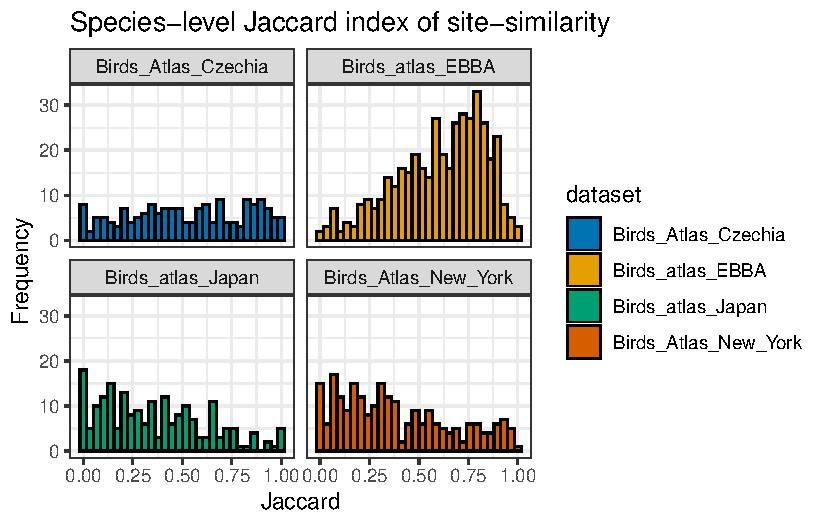
\includegraphics{MachineLearning_StaticPatterNN_Report_files/figure-pdf/raw-visualization-1.pdf}

\begin{Shaded}
\begin{Highlighting}[]
\FunctionTok{featurePlot}\NormalTok{(}
    \AttributeTok{x =}\NormalTok{ dat }\SpecialCharTok{\%\textgreater{}\%} \FunctionTok{select}\NormalTok{(dataset, }\FunctionTok{all\_of}\NormalTok{(H1\_vars)),}
    \AttributeTok{y =}\NormalTok{ dat}\SpecialCharTok{$}\NormalTok{Jaccard,}
    \AttributeTok{group =}\NormalTok{ dat}\SpecialCharTok{$}\NormalTok{dataset,}
    \AttributeTok{plot =} \StringTok{"pairs"}\NormalTok{,}
    \AttributeTok{pch =} \DecValTok{16}\NormalTok{,}
    \AttributeTok{alpha =} \FloatTok{0.3}\NormalTok{,}
    \AttributeTok{cex =} \FloatTok{0.2}\NormalTok{,}
    \AttributeTok{xlab =} \StringTok{"Scatterplot Matrix of species predictors"}\NormalTok{,}
    \AttributeTok{par.settings =}
        \FunctionTok{list}\NormalTok{(}
            \AttributeTok{fontsize =} \FunctionTok{list}\NormalTok{(}\AttributeTok{text =} \DecValTok{4}\NormalTok{)}
\NormalTok{        )}
\NormalTok{)}
\end{Highlighting}
\end{Shaded}

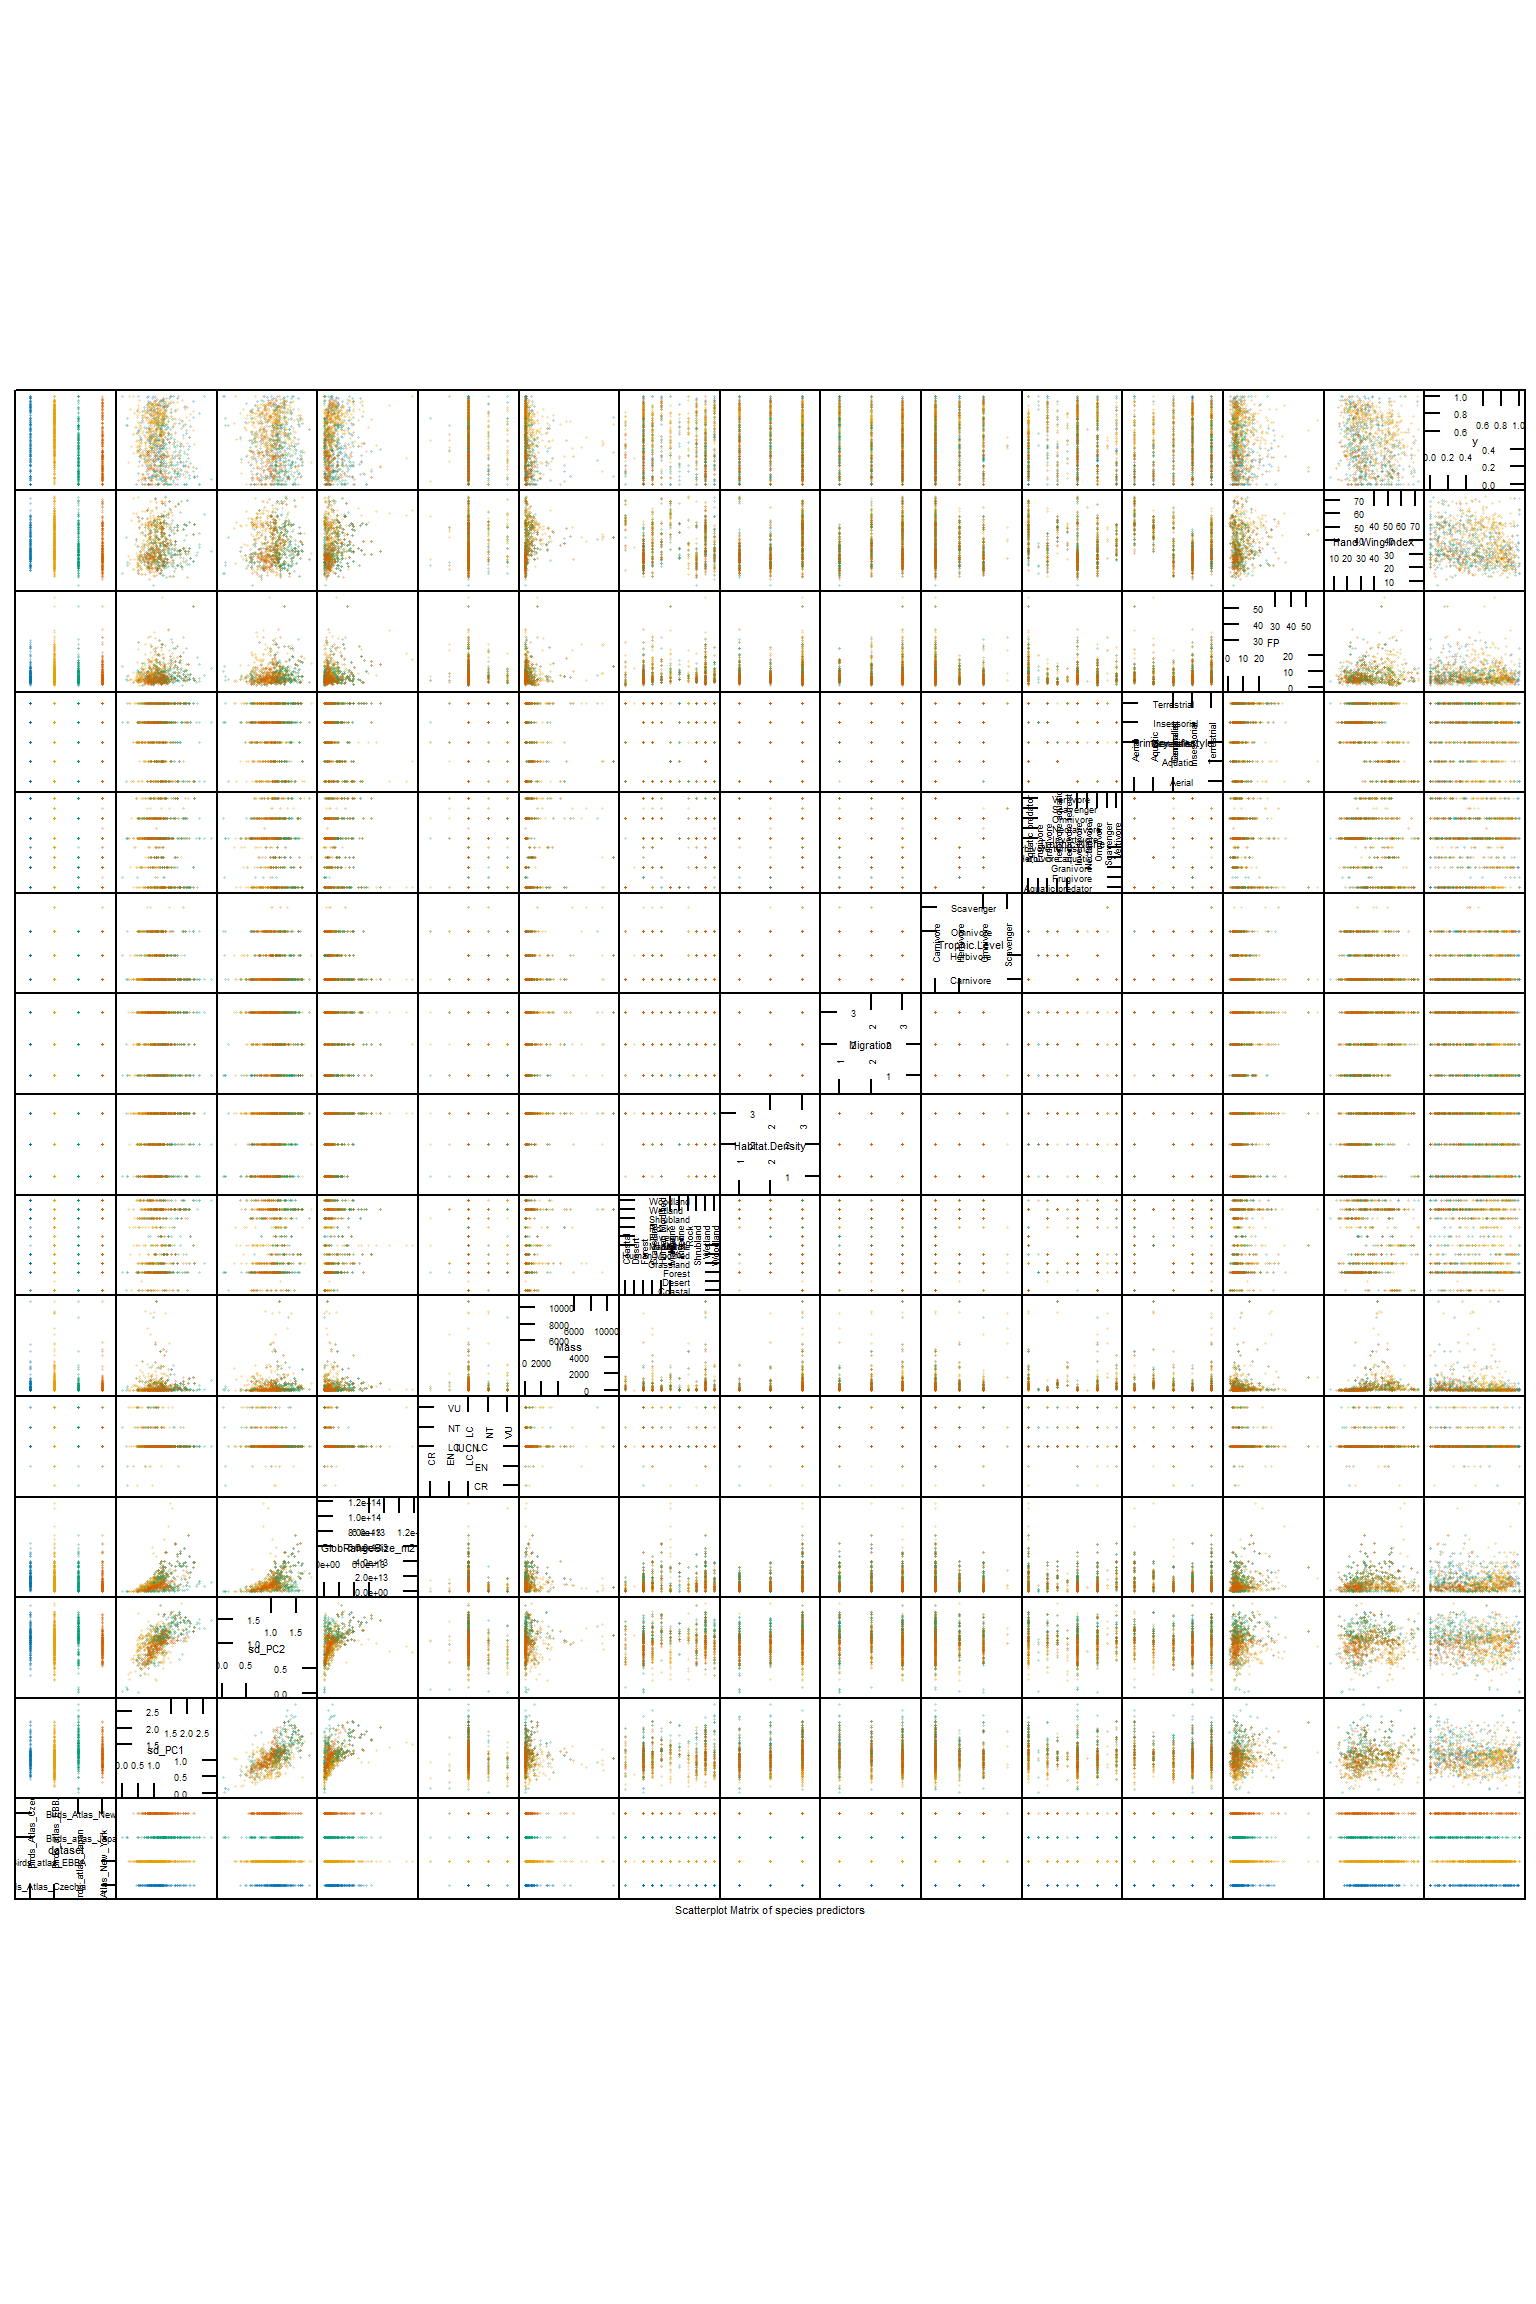
\includegraphics{MachineLearning_StaticPatterNN_Report_files/figure-pdf/feature-plots-1.pdf}

\begin{Shaded}
\begin{Highlighting}[]
\FunctionTok{featurePlot}\NormalTok{(}
    \AttributeTok{x =}\NormalTok{ dat }\SpecialCharTok{\%\textgreater{}\%} \FunctionTok{select}\NormalTok{(dataset, }\FunctionTok{all\_of}\NormalTok{(H2\_vars)),}
    \AttributeTok{y =}\NormalTok{ dat}\SpecialCharTok{$}\NormalTok{Jaccard,}
    \AttributeTok{group =}\NormalTok{ dat}\SpecialCharTok{$}\NormalTok{dataset,}
    \AttributeTok{plot =} \StringTok{"pairs"}\NormalTok{,}
    \AttributeTok{pch =} \DecValTok{16}\NormalTok{,}
    \AttributeTok{alpha =} \FloatTok{0.3}\NormalTok{,}
    \AttributeTok{cex =} \FloatTok{0.2}\NormalTok{,}
    \AttributeTok{xlab =} \StringTok{"Scatterplot Matrix of species geometry"}\NormalTok{,}
    \AttributeTok{par.settings =}
        \FunctionTok{list}\NormalTok{(}
            \AttributeTok{fontsize =} \FunctionTok{list}\NormalTok{(}\AttributeTok{text =} \DecValTok{4}\NormalTok{)}
\NormalTok{        )}
\NormalTok{)}
\end{Highlighting}
\end{Shaded}

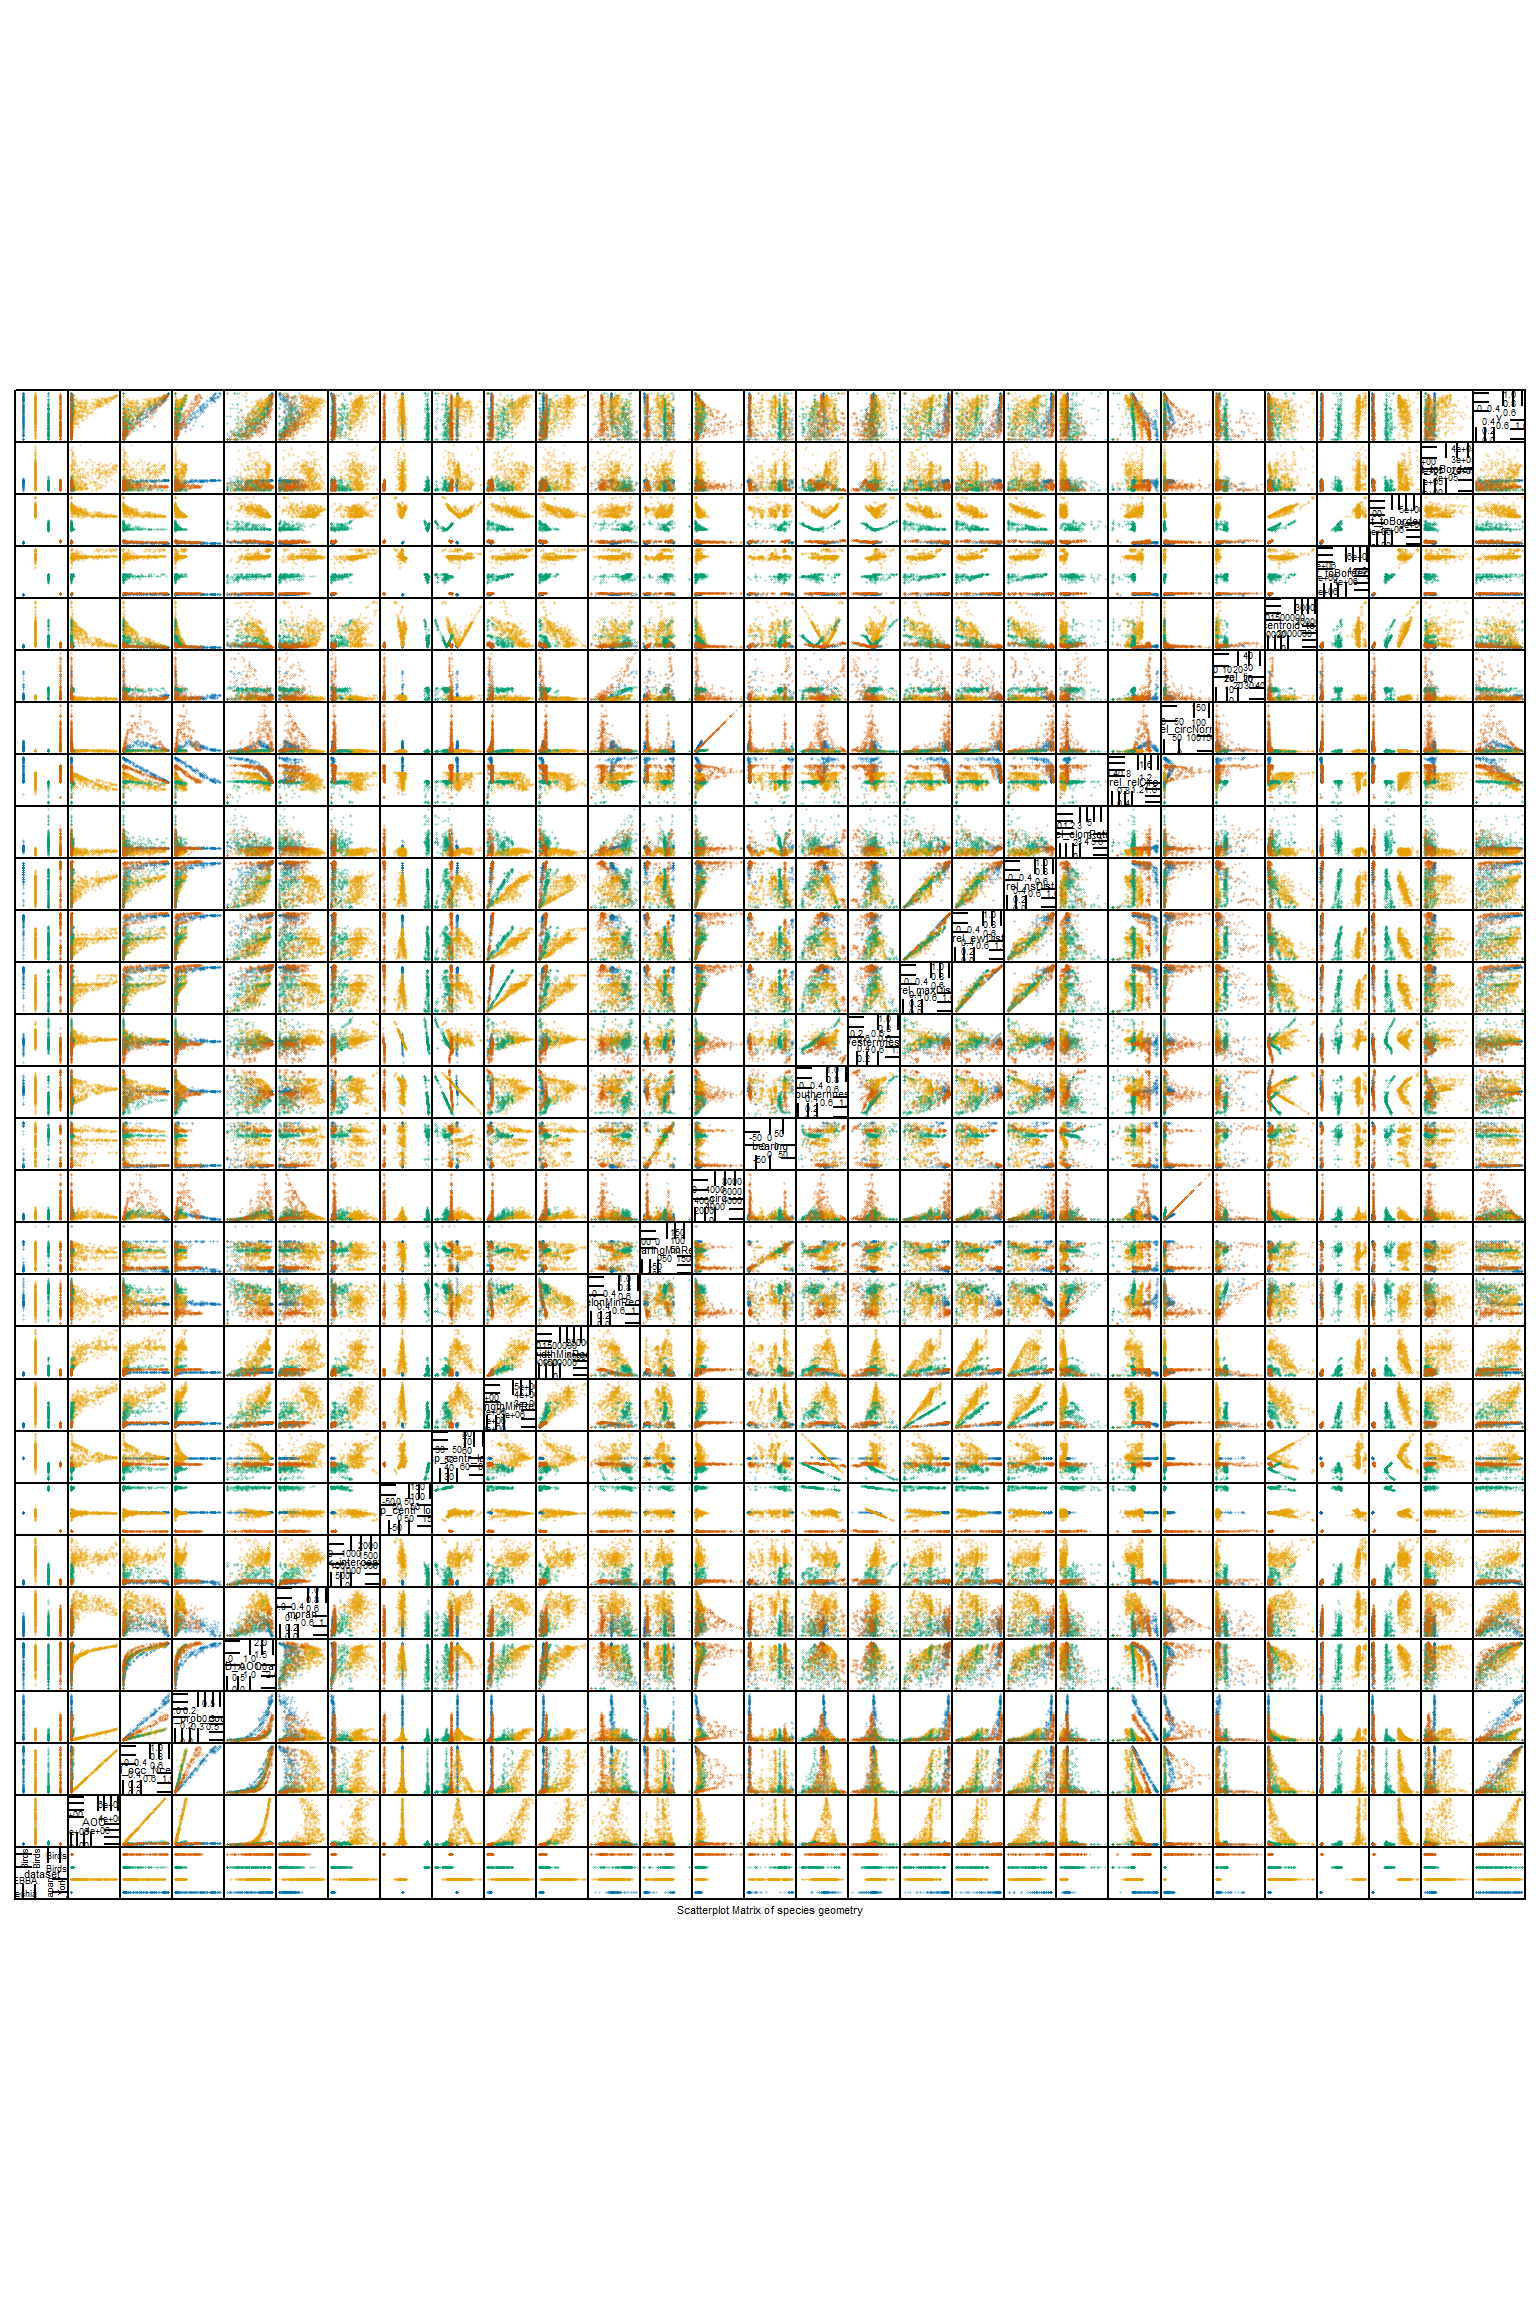
\includegraphics{MachineLearning_StaticPatterNN_Report_files/figure-pdf/feature-plots-2.pdf}

\begin{Shaded}
\begin{Highlighting}[]
\FunctionTok{featurePlot}\NormalTok{(}
    \AttributeTok{x =}\NormalTok{ dat }\SpecialCharTok{\%\textgreater{}\%} \FunctionTok{select}\NormalTok{(dataset, }\FunctionTok{all\_of}\NormalTok{(H3\_vars)),}
    \AttributeTok{y =}\NormalTok{ dat}\SpecialCharTok{$}\NormalTok{Jaccard,}
    \AttributeTok{group =}\NormalTok{ dat}\SpecialCharTok{$}\NormalTok{dataset,}
    \AttributeTok{plot =} \StringTok{"pairs"}\NormalTok{,}
    \AttributeTok{pch =} \DecValTok{16}\NormalTok{,}
    \AttributeTok{alpha =} \FloatTok{0.3}\NormalTok{,}
    \AttributeTok{cex =} \FloatTok{0.2}\NormalTok{,}
    \AttributeTok{xlab =} \StringTok{"Scatterplot Matrix of diversity metrics"}\NormalTok{,}
    \AttributeTok{par.settings =}
        \FunctionTok{list}\NormalTok{(}
            \AttributeTok{fontsize =} \FunctionTok{list}\NormalTok{(}\AttributeTok{text =} \DecValTok{4}\NormalTok{)}
\NormalTok{        )}
\NormalTok{)}
\end{Highlighting}
\end{Shaded}

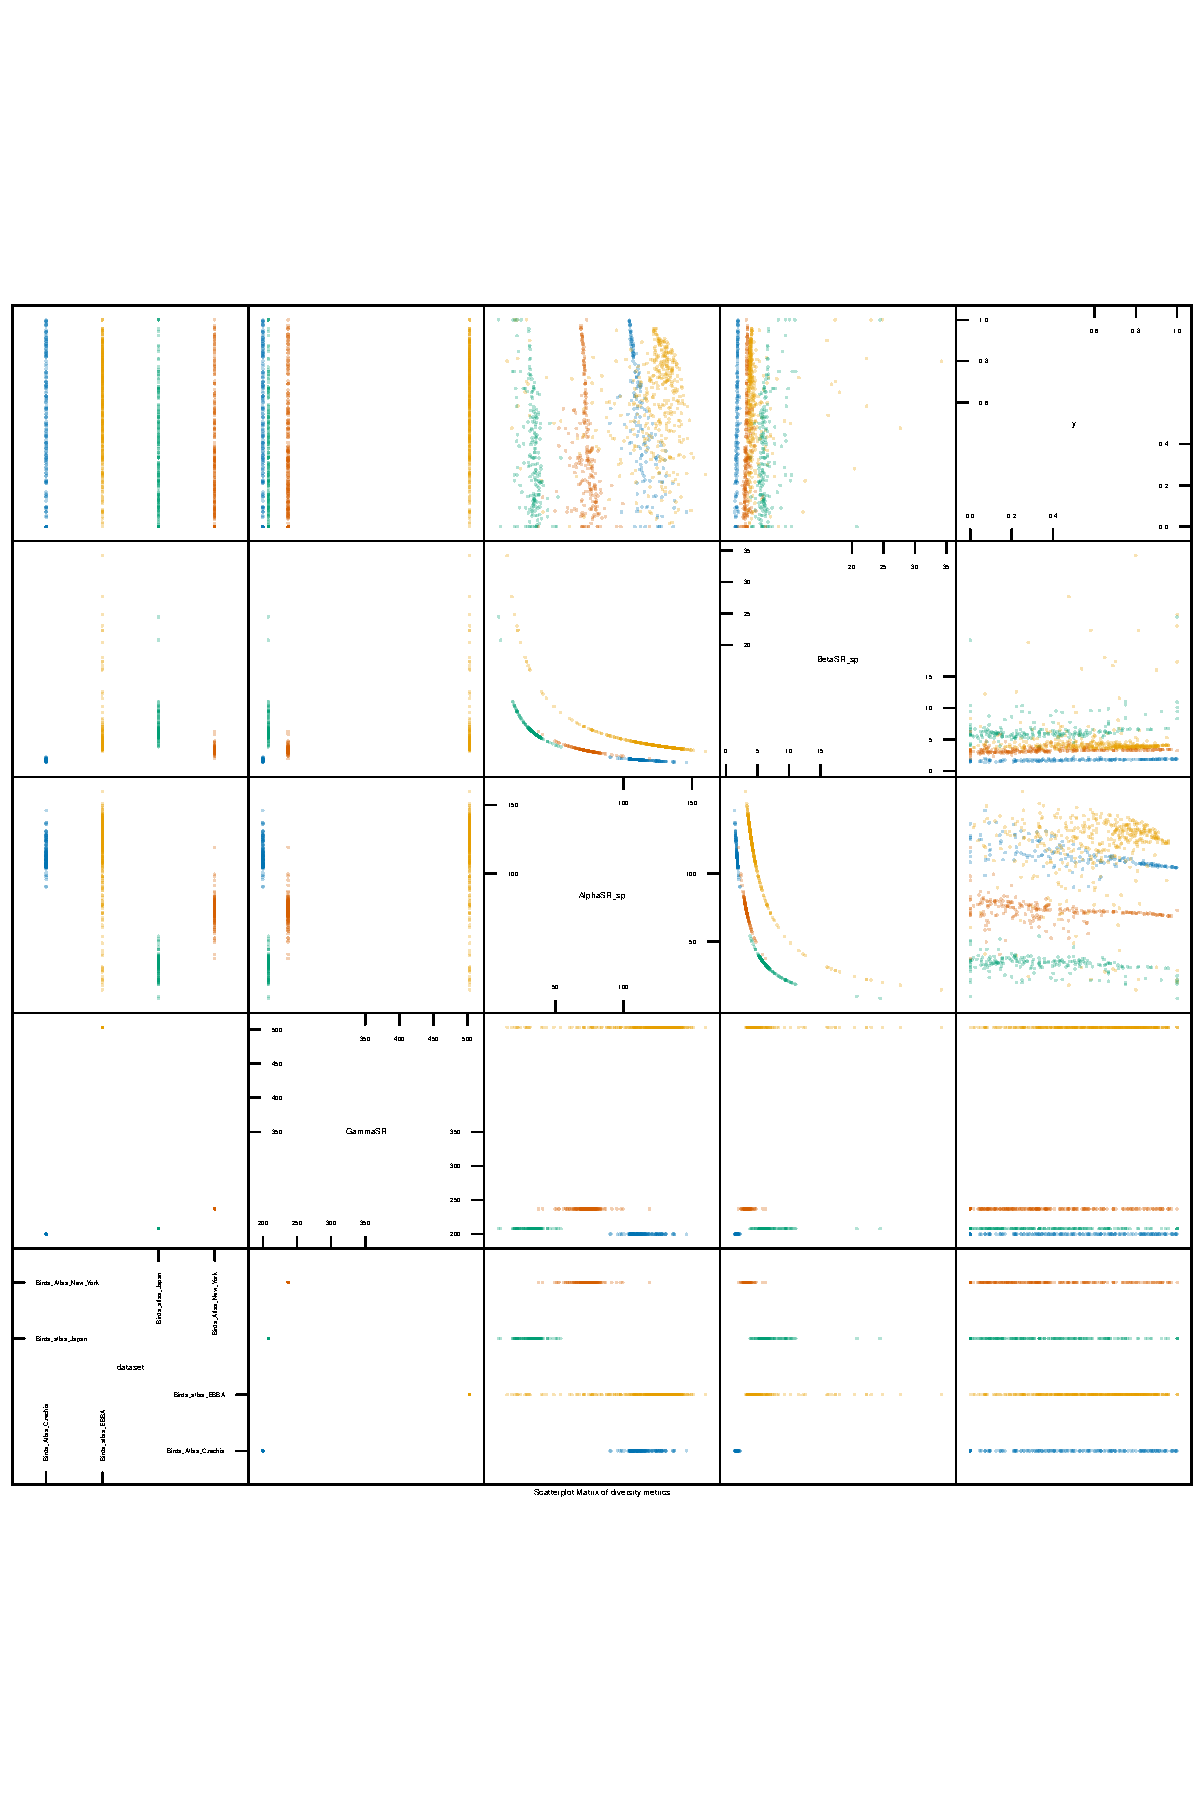
\includegraphics{MachineLearning_StaticPatterNN_Report_files/figure-pdf/feature-plots-3.pdf}

\begin{Shaded}
\begin{Highlighting}[]
\FunctionTok{featurePlot}\NormalTok{(}
    \AttributeTok{x =}\NormalTok{ dat }\SpecialCharTok{\%\textgreater{}\%} \FunctionTok{select}\NormalTok{(dataset, }\FunctionTok{all\_of}\NormalTok{(H4\_vars)),}
    \AttributeTok{y =}\NormalTok{ dat}\SpecialCharTok{$}\NormalTok{Jaccard,}
    \AttributeTok{group =}\NormalTok{ dat}\SpecialCharTok{$}\NormalTok{dataset,}
    \AttributeTok{plot =} \StringTok{"pairs"}\NormalTok{,}
    \AttributeTok{pch =} \DecValTok{16}\NormalTok{,}
    \AttributeTok{alpha =} \FloatTok{0.6}\NormalTok{,}
    \AttributeTok{cex =} \FloatTok{0.2}\NormalTok{,}
    \AttributeTok{xlab =} \StringTok{"Scatterplot Matrix of atlas specifics"}\NormalTok{,}
    \AttributeTok{par.settings =}
        \FunctionTok{list}\NormalTok{(}
            \AttributeTok{fontsize =} \FunctionTok{list}\NormalTok{(}\AttributeTok{text =} \DecValTok{4}\NormalTok{)}
\NormalTok{        )}
\NormalTok{)}
\end{Highlighting}
\end{Shaded}

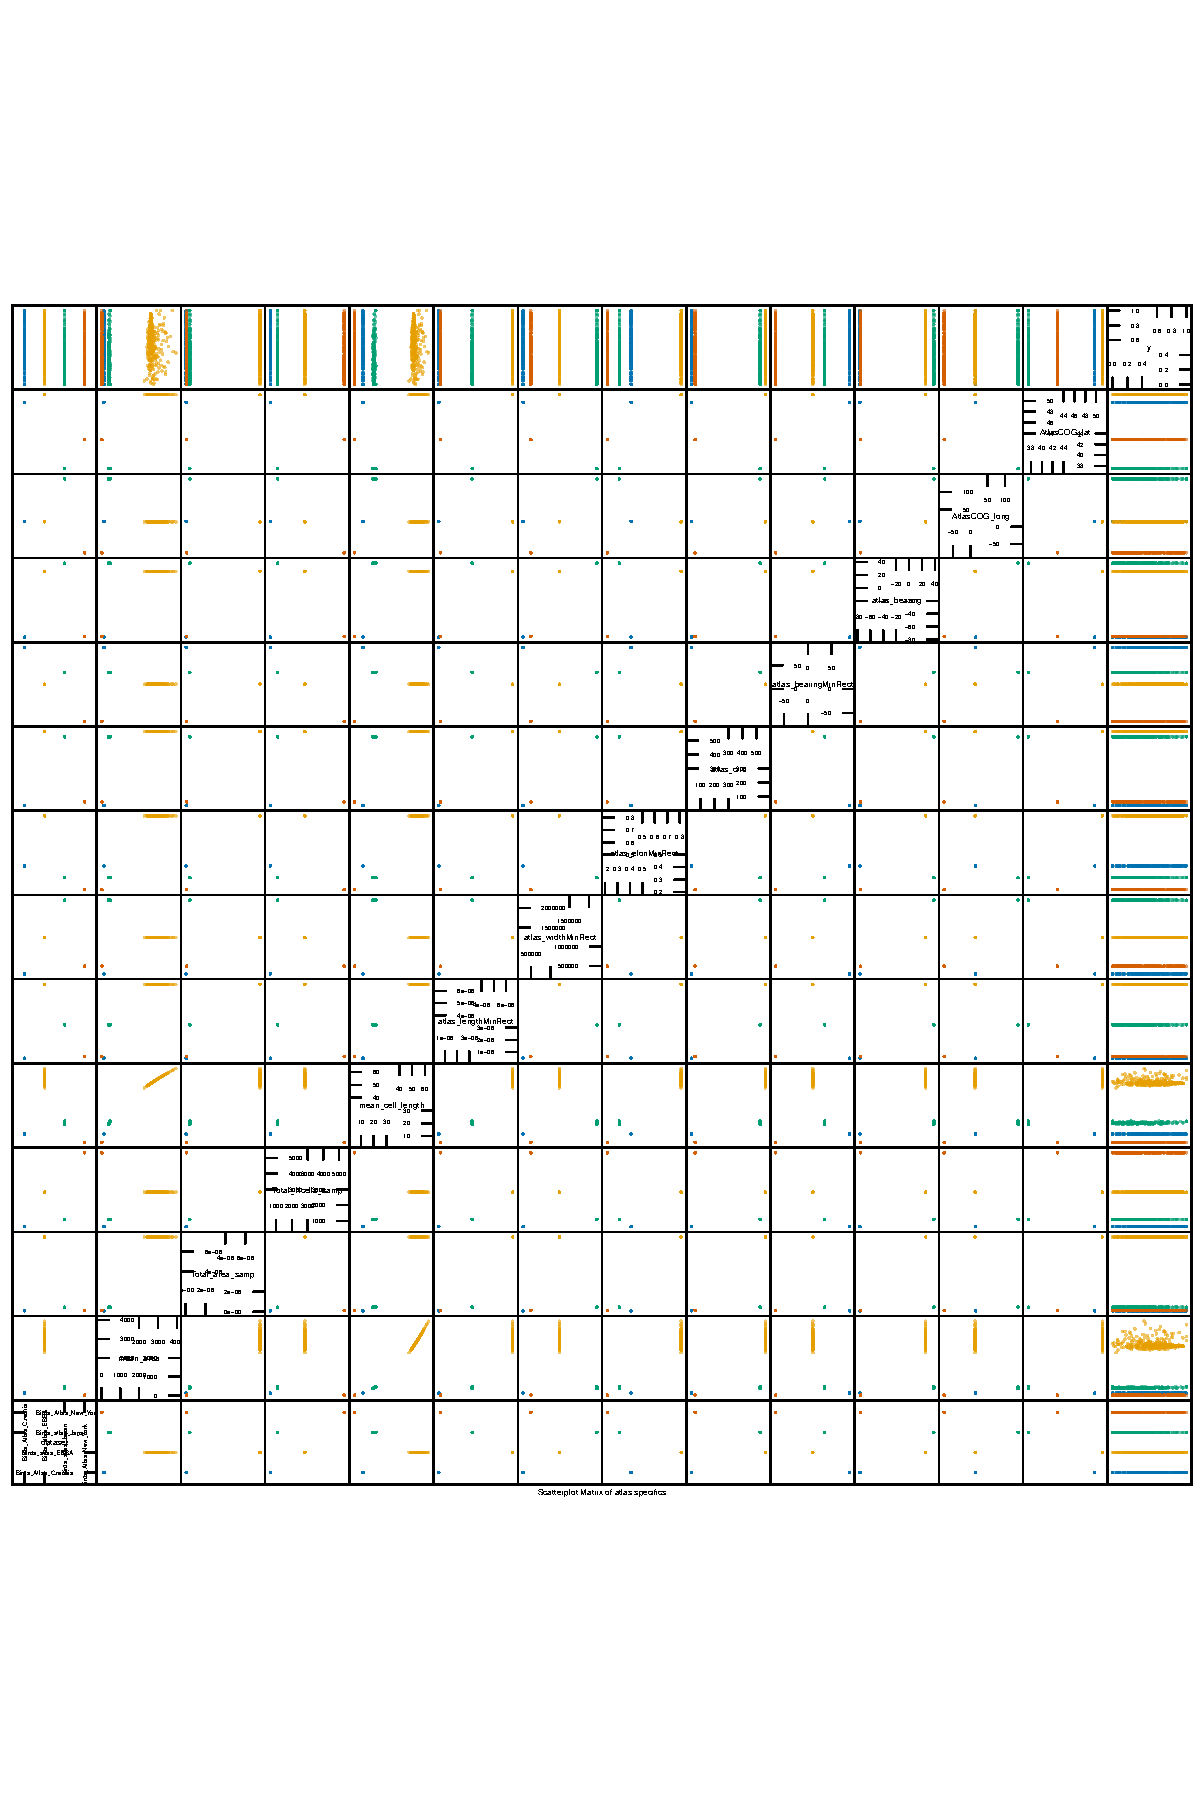
\includegraphics{MachineLearning_StaticPatterNN_Report_files/figure-pdf/feature-plots-4.pdf}

\begin{Shaded}
\begin{Highlighting}[]
\NormalTok{cor\_df }\OtherTok{\textless{}{-}}\NormalTok{ dat }\SpecialCharTok{\%\textgreater{}\%} \FunctionTok{select}\NormalTok{(}\SpecialCharTok{{-}}\NormalTok{Jaccard)}
\NormalTok{p.mat }\OtherTok{\textless{}{-}} \FunctionTok{model.matrix}\NormalTok{(}\SpecialCharTok{\textasciitilde{}} \DecValTok{0} \SpecialCharTok{+}\NormalTok{ ., }\AttributeTok{data =}\NormalTok{ cor\_df) }\SpecialCharTok{\%\textgreater{}\%}
    \FunctionTok{cor\_pmat}\NormalTok{()}

\NormalTok{correlation\_matrix }\OtherTok{\textless{}{-}}\NormalTok{ cor\_df }\SpecialCharTok{\%\textgreater{}\%}
    \FunctionTok{select\_if}\NormalTok{(is.numeric) }\SpecialCharTok{\%\textgreater{}\%}
    \FunctionTok{cor}\NormalTok{(}\AttributeTok{use =} \StringTok{"pairwise.complete.obs"}\NormalTok{)}
\NormalTok{correlation\_matrix }\SpecialCharTok{\%\textgreater{}\%}
    \FunctionTok{ggcorrplot}\NormalTok{(}
        \AttributeTok{hc.order =} \ConstantTok{TRUE}\NormalTok{,}
        \AttributeTok{lab =} \ConstantTok{TRUE}\NormalTok{,}
        \AttributeTok{lab\_size =} \DecValTok{3}\NormalTok{,}
        \AttributeTok{p.mat =}\NormalTok{ p.mat,}
        \AttributeTok{insig =} \StringTok{"blank"}
\NormalTok{    )}
\end{Highlighting}
\end{Shaded}

\includegraphics{MachineLearning_StaticPatterNN_Report_files/figure-pdf/correlation-matrix-1.pdf}

\begin{Shaded}
\begin{Highlighting}[]
\CommentTok{\# We will set the threshold for excluding correlations = 0.85}
\CommentTok{\# this is a bit arbitrary, trying to find a good trade{-}off between loss of predictor variables and collinearity}

\NormalTok{cor\_vars }\OtherTok{\textless{}{-}} \FunctionTok{findCorrelation}\NormalTok{(correlation\_matrix,}
    \AttributeTok{cutoff =}\NormalTok{ .}\DecValTok{85}\NormalTok{,}
    \AttributeTok{names =} \ConstantTok{TRUE}\NormalTok{,}
    \AttributeTok{exact =} \ConstantTok{TRUE}\NormalTok{,}
    \AttributeTok{verbose =} \ConstantTok{TRUE}
\NormalTok{)}
\end{Highlighting}
\end{Shaded}

\begin{verbatim}
Compare row 32  and column  41 with corr  0.98 
  Means:  0.469 vs 0.285 so flagging column 32 
Compare row 41  and column  40 with corr  0.981 
  Means:  0.458 vs 0.277 so flagging column 41 
Compare row 40  and column  31 with corr  0.975 
  Means:  0.446 vs 0.27 so flagging column 40 
Compare row 31  and column  37 with corr  0.952 
  Means:  0.432 vs 0.262 so flagging column 31 
Compare row 37  and column  43 with corr  0.969 
  Means:  0.4 vs 0.255 so flagging column 37 
Compare row 44  and column  46 with corr  0.989 
  Means:  0.395 vs 0.248 so flagging column 44 
Compare row 43  and column  38 with corr  0.972 
  Means:  0.375 vs 0.241 so flagging column 43 
Compare row 38  and column  34 with corr  0.995 
  Means:  0.353 vs 0.235 so flagging column 38 
Compare row 34  and column  12 with corr  0.866 
  Means:  0.335 vs 0.229 so flagging column 34 
Compare row 46  and column  42 with corr  0.886 
  Means:  0.351 vs 0.223 so flagging column 46 
Compare row 15  and column  16 with corr  0.881 
  Means:  0.266 vs 0.219 so flagging column 15 
Compare row 24  and column  25 with corr  0.927 
  Means:  0.313 vs 0.214 so flagging column 24 
Compare row 25  and column  23 with corr  0.953 
  Means:  0.288 vs 0.209 so flagging column 25 
Compare row 48  and column  35 with corr  0.891 
  Means:  0.293 vs 0.205 so flagging column 48 
Compare row 28  and column  19 with corr  0.926 
  Means:  0.245 vs 0.202 so flagging column 28 
Compare row 47  and column  13 with corr  0.996 
  Means:  0.29 vs 0.196 so flagging column 47 
Compare row 39  and column  45 with corr  0.971 
  Means:  0.178 vs 0.194 so flagging column 45 
All correlations <= 0.85 
\end{verbatim}

\begin{Shaded}
\begin{Highlighting}[]
\NormalTok{cor\_vars}
\end{Highlighting}
\end{Shaded}

\begin{verbatim}
 [1] "maxDist_toBorder_centr"  "atlas_lengthMinRect"    
 [3] "mean_cell_length"        "maxDist_toBorder_border"
 [5] "mean_area"               "atlas_circ"             
 [7] "atlas_elonMinRect"       "Total_area_samp"        
 [9] "GammaSR"                 "atlas_bearing"          
[11] "lengthMinRect"           "rel_ewDist"             
[13] "rel_nsDist"              "AtlasCOG_lat"           
[15] "rel_circNorm"            "AtlasCOG_long"          
[17] "atlas_bearingMinRect"   
\end{verbatim}

\begin{Shaded}
\begin{Highlighting}[]
\CommentTok{\# 13 variables seemed to be highly correlated. We will exclude}

\NormalTok{model\_dat }\OtherTok{\textless{}{-}}\NormalTok{ dat }\SpecialCharTok{\%\textgreater{}\%}
    \FunctionTok{select}\NormalTok{(}\SpecialCharTok{!}\FunctionTok{all\_of}\NormalTok{(cor\_vars))}

\FunctionTok{colSums}\NormalTok{(}\FunctionTok{is.na}\NormalTok{(model\_dat))}
\end{Highlighting}
\end{Shaded}

\begin{verbatim}
               Jaccard                 sd_PC1                 sd_PC2 
                     0                      2                      2 
      GlobRangeSize_m2                   IUCN                   Mass 
                     2                      3                      3 
               Habitat        Habitat.Density              Migration 
                     3                      3                      3 
         Trophic.Level          Trophic.Niche      Primary.Lifestyle 
                     3                      3                      3 
                    FP        Hand.Wing.Index                    AOO 
                     0                      3                      0 
        rel_occ_Ncells      mean_prob_cooccur                D_AOO_a 
                     0                      3                      0 
                 moran            x_intercept           sp_centr_lon 
                     0                      0                      0 
          sp_centr_lat           widthMinRect            elonMinRect 
                     0                      0                      0 
        bearingMinRect                   circ                bearing 
                     0                      0                      0 
          Southernness            Westernness            rel_maxDist 
                     0                      0                      0 
         rel_elonRatio            rel_relCirc                rel_lin 
                     0                      0                      0 
  Dist_centroid_to_COG minDist_toBorder_centr             AlphaSR_sp 
                     0                      0                      0 
             BetaSR_sp                dataset      Total_Ncells_samp 
                     0                      0                      0 
    atlas_widthMinRect 
                     0 
\end{verbatim}

\begin{Shaded}
\begin{Highlighting}[]
\CommentTok{\# leaves us with 39 predictor variables to predict Jaccard similarity index}
\end{Highlighting}
\end{Shaded}

\subsection{Modeling}\label{modeling}

\subsubsection{Pre-processing:}\label{pre-processing}

First we have to check if there are (near) zero variance variables in
the predictors. These can be removed since they will not explain a lot
generally.

Second, we will exclude all correlated variables with pearson's pairwise
correlations coefficients \textgreater{} 0.85.

Third, we will impute NA values based on knn-imputation with 5 neighbors
(default).

\begin{Shaded}
\begin{Highlighting}[]
\CommentTok{\# Step 1. Near Zero Vars}
\NormalTok{nzv }\OtherTok{\textless{}{-}} \FunctionTok{nearZeroVar}\NormalTok{(model\_dat, }\AttributeTok{saveMetrics =}\NormalTok{ T)}
\NormalTok{nzv }\SpecialCharTok{\%\textgreater{}\%} \FunctionTok{filter}\NormalTok{(nzv }\SpecialCharTok{==}\NormalTok{ T)}
\end{Highlighting}
\end{Shaded}

\begin{verbatim}
     freqRatio percentUnique zeroVar  nzv
IUCN   19.4375     0.4854369   FALSE TRUE
\end{verbatim}

\begin{Shaded}
\begin{Highlighting}[]
\CommentTok{\# only IUCN, but this is an important predictor (!) we will keep it.}

\CommentTok{\# Step 2 \& 3: imputing missing values \& removing highly correlated variables}
\NormalTok{recipe\_pp }\OtherTok{\textless{}{-}} \FunctionTok{recipe}\NormalTok{(Jaccard }\SpecialCharTok{\textasciitilde{}}\NormalTok{ .,}
    \AttributeTok{data =}\NormalTok{ dat}
\NormalTok{) }\SpecialCharTok{\%\textgreater{}\%}
    \FunctionTok{step\_corr}\NormalTok{(}\FunctionTok{all\_numeric\_predictors}\NormalTok{(), }\AttributeTok{threshold =}\NormalTok{ .}\DecValTok{85}\NormalTok{) }\SpecialCharTok{\%\textgreater{}\%}
    \FunctionTok{step\_impute\_knn}\NormalTok{(}\FunctionTok{all\_predictors}\NormalTok{())}

\CommentTok{\# Estimate recipe on data:}
\NormalTok{recipe\_pp\_prepped }\OtherTok{\textless{}{-}} \FunctionTok{prep}\NormalTok{(recipe\_pp, dat)}

\CommentTok{\# Removed columns:}
\NormalTok{recipe\_pp\_prepped}\SpecialCharTok{$}\NormalTok{steps[[}\DecValTok{1}\NormalTok{]]}\SpecialCharTok{$}\NormalTok{removals}
\end{Highlighting}
\end{Shaded}

\begin{verbatim}
 [1] "rel_ewDist"              "rel_nsDist"             
 [3] "rel_circNorm"            "maxDist_toBorder_border"
 [5] "maxDist_toBorder_centr"  "GammaSR"                
 [7] "mean_area"               "Total_area_samp"        
 [9] "mean_cell_length"        "atlas_lengthMinRect"    
[11] "atlas_elonMinRect"       "atlas_bearing"          
[13] "AtlasCOG_long"           "AtlasCOG_lat"           
[15] "lengthMinRect"           "Total_Ncells_samp"      
[17] "atlas_circ"             
\end{verbatim}

\begin{Shaded}
\begin{Highlighting}[]
\CommentTok{\# apply the recipe to the data:}
\NormalTok{dat\_v2 }\OtherTok{\textless{}{-}} \FunctionTok{bake}\NormalTok{(recipe\_pp\_prepped, dat)}
\end{Highlighting}
\end{Shaded}

\subsubsection{Training \& Validation
sets:}\label{training-validation-sets}

\begin{Shaded}
\begin{Highlighting}[]
\FunctionTok{set.seed}\NormalTok{(}\DecValTok{42}\NormalTok{)}
\CommentTok{\# Initial split to training and validation set (for final evaluation, keep dat\_test completely out of the training sets)}
\NormalTok{index }\OtherTok{\textless{}{-}} \FunctionTok{createDataPartition}\NormalTok{(dat\_v2}\SpecialCharTok{$}\NormalTok{Jaccard, }\AttributeTok{p =} \FloatTok{0.8}\NormalTok{, }\DecValTok{1}\NormalTok{, }\AttributeTok{list =} \ConstantTok{FALSE}\NormalTok{)}

\NormalTok{dat\_train }\OtherTok{\textless{}{-}}\NormalTok{ dat\_v2[index, ]}
\NormalTok{dat\_test }\OtherTok{\textless{}{-}}\NormalTok{ dat\_v2[}\SpecialCharTok{{-}}\NormalTok{index, ]}

\CommentTok{\# Cross{-}validation resampling indices }
\NormalTok{indices }\OtherTok{\textless{}{-}} \FunctionTok{createDataPartition}\NormalTok{(dat\_train}\SpecialCharTok{$}\NormalTok{Jaccard, }\AttributeTok{p =} \FloatTok{0.8}\NormalTok{, }\DecValTok{10}\NormalTok{) }\CommentTok{\# 10 resamples}
\end{Highlighting}
\end{Shaded}

\subsubsection{Variation Partitioning between
Hypotheses}\label{variation-partitioning-between-hypotheses}

\begin{Shaded}
\begin{Highlighting}[]
\CommentTok{\# Create a data frame for each set of variables}
\NormalTok{H1\_data }\OtherTok{\textless{}{-}}\NormalTok{ dat\_train }\SpecialCharTok{\%\textgreater{}\%} \FunctionTok{select}\NormalTok{(}\FunctionTok{any\_of}\NormalTok{(H1\_vars))}
\NormalTok{H2\_data }\OtherTok{\textless{}{-}}\NormalTok{ dat\_train }\SpecialCharTok{\%\textgreater{}\%} \FunctionTok{select}\NormalTok{(}\FunctionTok{any\_of}\NormalTok{(H2\_vars))}
\NormalTok{H3\_data }\OtherTok{\textless{}{-}}\NormalTok{ dat\_train }\SpecialCharTok{\%\textgreater{}\%} \FunctionTok{select}\NormalTok{(}\FunctionTok{any\_of}\NormalTok{(H3\_vars))}
\NormalTok{H4\_data }\OtherTok{\textless{}{-}}\NormalTok{ dat\_train }\SpecialCharTok{\%\textgreater{}\%} \FunctionTok{select}\NormalTok{(}\FunctionTok{any\_of}\NormalTok{(H4\_vars))}

\CommentTok{\# Perform basic variation partitioning (vegan package)}
\NormalTok{varpart\_model }\OtherTok{\textless{}{-}} \FunctionTok{varpart}\NormalTok{(dat\_train}\SpecialCharTok{$}\NormalTok{Jaccard, H1\_data, H2\_data, H3\_data, H4\_data)}
\end{Highlighting}
\end{Shaded}

\begin{verbatim}
Warning: collinearity detected in X1: mm = 40, m = 39
\end{verbatim}

\begin{verbatim}
Warning: collinearity detected in X4: mm = 5, m = 3
\end{verbatim}

\begin{verbatim}
Warning: collinearity detected in cbind(X1,X2): mm = 61, m = 60
\end{verbatim}

\begin{verbatim}
Warning: collinearity detected in cbind(X1,X3: mm = 42, m = 41
\end{verbatim}

\begin{verbatim}
Warning: collinearity detected in cbind(X1,X4): mm = 45, m = 42
\end{verbatim}

\begin{verbatim}
Warning: collinearity detected in cbind(X2,X4): mm = 26, m = 24
\end{verbatim}

\begin{verbatim}
Warning: collinearity detected in cbind(X3,X4): mm = 7, m = 5
\end{verbatim}

\begin{verbatim}
Warning: collinearity detected in cbind(X1,X2,X3): mm = 63, m = 62
\end{verbatim}

\begin{verbatim}
Warning: collinearity detected in c(X1,X2,X4): mm = 66, m = 63
\end{verbatim}

\begin{verbatim}
Warning: collinearity detected in cbind(X1,X3,X4): mm = 47, m = 44
\end{verbatim}

\begin{verbatim}
Warning: collinearity detected in cbind(X2,X3,X4): mm = 28, m = 26
\end{verbatim}

\begin{verbatim}
Warning: collinearity detected in cbind(X1,X2,X3,X4): mm = 68, m = 65
\end{verbatim}

\begin{Shaded}
\begin{Highlighting}[]
\CommentTok{\# Print the results}
\FunctionTok{print}\NormalTok{(varpart\_model)}
\end{Highlighting}
\end{Shaded}

\begin{verbatim}

Partition of variance in RDA 

Call: varpart(Y = dat_train$Jaccard, X = H1_data, H2_data, H3_data,
H4_data)

Explanatory tables:
X1:  H1_data
X2:  H2_data
X3:  H3_data
X4:  H4_data 

No. of explanatory tables: 4 
Total variation (SS): 65.95 
            Variance: 0.07994 
No. of observations: 826 

Partition table:
                            Df R.square Adj.R.square Testable
[aeghklno] = X1             39  0.15029      0.10813     TRUE
[befiklmo] = X2             21  0.81155      0.80663     TRUE
[cfgjlmno] = X3              2  0.12706      0.12494     TRUE
[dhijkmno] = X4              3  0.15349      0.15040     TRUE
[abefghiklmno] = X1+X2      60  0.84221      0.82983     TRUE
[acefghjklmno] = X1+X3      41  0.29752      0.26078     TRUE
[adeghijklmno] = X1+X4      42  0.33364      0.29790     TRUE
[bcefgijklmno] = X2+X3      23  0.82133      0.81621     TRUE
[bdefhijklmno] = X2+X4      24  0.82251      0.81720     TRUE
[cdfghijklmno] = X3+X4       5  0.16202      0.15691     TRUE
[abcefghijklmno] = X1+X2+X3 62  0.84667      0.83421     TRUE
[abdefghijklmno] = X1+X2+X4 63  0.84915      0.83668     TRUE
[acdefghijklmno] = X1+X3+X4 44  0.34243      0.30538     TRUE
[bcdefghijklmno] = X2+X3+X4 26  0.83088      0.82538     TRUE
[abcdefghijklmno] = All     65  0.85386      0.84136     TRUE
Individual fractions                                         
[a] = X1 | X2+X3+X4         39               0.01598     TRUE
[b] = X2 | X1+X3+X4         21               0.53597     TRUE
[c] = X3 | X1+X2+X4          2               0.00468     TRUE
[d] = X4 | X1+X2+X3          3               0.00714     TRUE
[e]                          0               0.13250    FALSE
[f]                          0               0.00281    FALSE
[g]                          0               0.00350    FALSE
[h]                          0               0.00203    FALSE
[i]                          0               0.03746    FALSE
[j]                          0              -0.00030    FALSE
[k]                          0              -0.01466    FALSE
[l]                          0              -0.00448    FALSE
[m]                          0               0.14546    FALSE
[n]                          0               0.00170    FALSE
[o]                          0              -0.02843    FALSE
[p] = Residuals              0               0.15864    FALSE
Controlling 2 tables X                                       
[ae] = X1 | X3+X4           39               0.14848     TRUE
[ag] = X1 | X2+X4           39               0.01948     TRUE
[ah] = X1 | X2+X3           39               0.01801     TRUE
[be] = X2 | X3+X4           21               0.66847     TRUE
[bf] = X2 | X1+X4           21               0.53878     TRUE
[bi] = X2 | X1+X3           21               0.57344     TRUE
[cf] = X3 | X1+X4            2               0.00749     TRUE
[cg] = X3 | X2+X4            2               0.00818     TRUE
[cj] = X3 | X1+X2            2               0.00438     TRUE
[dh] = X4 | X2+X3            3               0.00917     TRUE
[di] = X4 | X1+X3            3               0.04461     TRUE
[dj] = X4 | X1+X2            3               0.00685     TRUE
Controlling 1 table X                                        
[aghn] = X1 | X2            39               0.02321     TRUE
[aehk] = X1 | X3            39               0.13584     TRUE
[aegl] = X1 | X4            39               0.14750     TRUE
[bfim] = X2 | X1            21               0.72170     TRUE
[beik] = X2 | X3            21               0.69127     TRUE
[befl] = X2 | X4            21               0.66680     TRUE
[cfjm] = X3 | X1             2               0.15265     TRUE
[cgjn] = X3 | X2             2               0.00958     TRUE
[cfgl] = X3 | X4             2               0.00651     TRUE
[dijm] = X4 | X1             3               0.18977     TRUE
[dhjn] = X4 | X2             3               0.01057     TRUE
[dhik] = X4 | X3             3               0.03197     TRUE
---
Use function 'rda' to test significance of fractions of interest
\end{verbatim}

\begin{Shaded}
\begin{Highlighting}[]
\FunctionTok{summary}\NormalTok{(varpart\_model)}
\end{Highlighting}
\end{Shaded}

\begin{verbatim}

Unique fractions and total with shared fractions equally allocated:

    Unique Contributed Component
X1 0.01598      0.0721   H1_data
X2 0.53597      0.6574   H2_data
X3 0.00468      0.0481   H3_data
X4 0.00714      0.0638   H4_data

Contributions of fractions to sets:

           X1        X2        X3        X4
[a]  0.015981                              
[b]            0.535973                    
[c]                      0.004677          
[d]                                0.007142
[e]  0.066249  0.066249                    
[f]            0.001405  0.001405          
[g]  0.001751            0.001751          
[h]  0.001014                      0.001014
[i]            0.018732            0.018732
[j]                     -0.000148 -0.000148
[k] -0.004888 -0.004888           -0.004888
[l] -0.001494 -0.001494 -0.001494          
[m]            0.048486  0.048486  0.048486
[n]  0.000566            0.000566  0.000566
[o] -0.007108 -0.007108 -0.007108 -0.007108
\end{verbatim}

\begin{Shaded}
\begin{Highlighting}[]
\DocumentationTok{\#\# VENN{-}diagram}
\FunctionTok{plot}\NormalTok{(varpart\_model,}
     \AttributeTok{Xnames =} \FunctionTok{c}\NormalTok{(}\StringTok{"Species Traits"}\NormalTok{, }\StringTok{"Species Range Geometry"}\NormalTok{, }\StringTok{"Diversity"}\NormalTok{, }\StringTok{"Atlas characteristics"}\NormalTok{), }\CommentTok{\# name the partitions}
     \AttributeTok{bg =} \FunctionTok{c}\NormalTok{(}\StringTok{"seagreen3"}\NormalTok{, }\StringTok{"mediumpurple"}\NormalTok{, }\StringTok{"darkorange"}\NormalTok{, }\StringTok{"gold"}\NormalTok{), }\AttributeTok{alpha =} \DecValTok{80}\NormalTok{, }\CommentTok{\# colour the circles}
     \AttributeTok{digits =} \DecValTok{2}\NormalTok{, }\CommentTok{\# only show 2 digits}
     \AttributeTok{cex =} \FloatTok{0.8}\NormalTok{,}
     \AttributeTok{id.size =} \DecValTok{1}\NormalTok{)}
\end{Highlighting}
\end{Shaded}

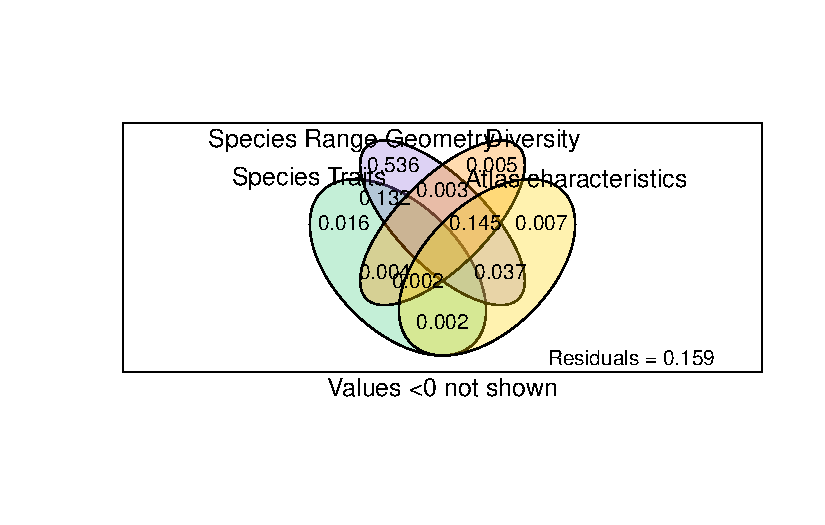
\includegraphics{MachineLearning_StaticPatterNN_Report_files/figure-pdf/var-part-vegan-1.pdf}

\begin{Shaded}
\begin{Highlighting}[]
\CommentTok{\# Test for significance in results:}
\FunctionTok{anova.cca}\NormalTok{(}\FunctionTok{rda}\NormalTok{(dat\_train}\SpecialCharTok{$}\NormalTok{Jaccard, H1\_data)) }\CommentTok{\# sign. p = 0.001}
\end{Highlighting}
\end{Shaded}

\begin{verbatim}
Permutation test for rda under reduced model
Permutation: free
Number of permutations: 999

Model: rda(X = dat_train$Jaccard, Y = H1_data)
          Df Variance      F Pr(>F)    
Model     39 0.012014 3.5647  0.001 ***
Residual 786 0.067925                  
---
Signif. codes:  0 '***' 0.001 '**' 0.01 '*' 0.05 '.' 0.1 ' ' 1
\end{verbatim}

\begin{Shaded}
\begin{Highlighting}[]
\FunctionTok{anova.cca}\NormalTok{(}\FunctionTok{rda}\NormalTok{(dat\_train}\SpecialCharTok{$}\NormalTok{Jaccard, H2\_data)) }\CommentTok{\# sign. p = 0.001}
\end{Highlighting}
\end{Shaded}

\begin{verbatim}
Permutation test for rda under reduced model
Permutation: free
Number of permutations: 999

Model: rda(X = dat_train$Jaccard, Y = H2_data)
          Df Variance      F Pr(>F)    
Model     21 0.064875 164.87  0.001 ***
Residual 804 0.015065                  
---
Signif. codes:  0 '***' 0.001 '**' 0.01 '*' 0.05 '.' 0.1 ' ' 1
\end{verbatim}

\begin{Shaded}
\begin{Highlighting}[]
\FunctionTok{anova.cca}\NormalTok{(}\FunctionTok{rda}\NormalTok{(dat\_train}\SpecialCharTok{$}\NormalTok{Jaccard, H3\_data)) }\CommentTok{\# sign. p = 0.001}
\end{Highlighting}
\end{Shaded}

\begin{verbatim}
Permutation test for rda under reduced model
Permutation: free
Number of permutations: 999

Model: rda(X = dat_train$Jaccard, Y = H3_data)
          Df Variance      F Pr(>F)    
Model      2 0.010157 59.894  0.001 ***
Residual 823 0.069783                  
---
Signif. codes:  0 '***' 0.001 '**' 0.01 '*' 0.05 '.' 0.1 ' ' 1
\end{verbatim}

\begin{Shaded}
\begin{Highlighting}[]
\FunctionTok{anova.cca}\NormalTok{(}\FunctionTok{rda}\NormalTok{(dat\_train}\SpecialCharTok{$}\NormalTok{Jaccard, H4\_data)) }\CommentTok{\# sign. p = 0.001}
\end{Highlighting}
\end{Shaded}

\begin{verbatim}
Permutation test for rda under reduced model
Permutation: free
Number of permutations: 999

Model: rda(X = dat_train$Jaccard, Y = H4_data)
          Df Variance      F Pr(>F)    
Model      3  0.01227 49.682  0.001 ***
Residual 822  0.06767                  
---
Signif. codes:  0 '***' 0.001 '**' 0.01 '*' 0.05 '.' 0.1 ' ' 1
\end{verbatim}

\begin{Shaded}
\begin{Highlighting}[]
\NormalTok{trainControl }\OtherTok{\textless{}{-}} \FunctionTok{trainControl}\NormalTok{(}
    \AttributeTok{method =} \StringTok{"repeatedcv"}\NormalTok{,}
    \AttributeTok{number =} \DecValTok{10}\NormalTok{,}
    \AttributeTok{repeats =} \DecValTok{3}\NormalTok{,}
    \AttributeTok{savePredictions =} \StringTok{"final"}\NormalTok{,}
    \AttributeTok{returnResamp =} \StringTok{"final"}\NormalTok{,}
    \AttributeTok{verboseIter =} \ConstantTok{TRUE}\NormalTok{,}
    \AttributeTok{index =}\NormalTok{ indices)}

\NormalTok{tictoc}\SpecialCharTok{::}\FunctionTok{tic}\NormalTok{(}\StringTok{"ranger full model"}\NormalTok{)}
\FunctionTok{set.seed}\NormalTok{(}\DecValTok{42}\NormalTok{)}
\NormalTok{full\_ranger }\OtherTok{\textless{}{-}} \FunctionTok{train}\NormalTok{(}
\NormalTok{    Jaccard }\SpecialCharTok{\textasciitilde{}}\NormalTok{ .,}
    \AttributeTok{data =}\NormalTok{ dat\_train,}
    \AttributeTok{method =} \StringTok{"ranger"}\NormalTok{,}
    \AttributeTok{trControl =}\NormalTok{ trainControl,}
    \AttributeTok{importance =} \StringTok{"permutation"}\NormalTok{,}
    \AttributeTok{scale.permutation.importance =} \ConstantTok{TRUE}\NormalTok{,}
    \AttributeTok{num.trees =} \DecValTok{5000}\NormalTok{,}
    \AttributeTok{respect.unordered.factors =} \ConstantTok{TRUE}\NormalTok{,}
    \AttributeTok{oob.error =} \ConstantTok{TRUE}\NormalTok{,}
    \AttributeTok{tuneLength =} \DecValTok{5}\NormalTok{)}
\NormalTok{tictoc}\SpecialCharTok{::}\FunctionTok{toc}\NormalTok{()}


\CommentTok{\# Train ranger model}
\NormalTok{tictoc}\SpecialCharTok{::}\FunctionTok{tic}\NormalTok{(}\StringTok{"ranger H1"}\NormalTok{)}
\FunctionTok{set.seed}\NormalTok{(}\DecValTok{42}\NormalTok{)}
\NormalTok{H1\_ranger }\OtherTok{\textless{}{-}} \FunctionTok{train}\NormalTok{(}
\NormalTok{    Jaccard }\SpecialCharTok{\textasciitilde{}}\NormalTok{ .,}
    \AttributeTok{data =}\NormalTok{ dat\_train }\SpecialCharTok{\%\textgreater{}\%} \FunctionTok{select}\NormalTok{(Jaccard, }\FunctionTok{any\_of}\NormalTok{(H1\_vars)),}
    \AttributeTok{method =} \StringTok{"ranger"}\NormalTok{,}
    \AttributeTok{trControl =}\NormalTok{ trainControl,}
    \AttributeTok{importance =} \StringTok{"permutation"}\NormalTok{,}
    \AttributeTok{scale.permutation.importance =} \ConstantTok{TRUE}\NormalTok{,}
    \AttributeTok{num.trees =} \DecValTok{5000}\NormalTok{,}
    \AttributeTok{respect.unordered.factors =} \ConstantTok{TRUE}\NormalTok{,}
    \AttributeTok{oob.error =} \ConstantTok{TRUE}\NormalTok{,}
    \AttributeTok{tuneLength =} \DecValTok{5}\NormalTok{)}
\NormalTok{tictoc}\SpecialCharTok{::}\FunctionTok{toc}\NormalTok{()}


\NormalTok{tictoc}\SpecialCharTok{::}\FunctionTok{tic}\NormalTok{(}\StringTok{"ranger H2"}\NormalTok{)}
\FunctionTok{set.seed}\NormalTok{(}\DecValTok{42}\NormalTok{)}
\NormalTok{H2\_ranger }\OtherTok{\textless{}{-}} \FunctionTok{train}\NormalTok{(}
\NormalTok{    Jaccard }\SpecialCharTok{\textasciitilde{}}\NormalTok{ .,}
    \AttributeTok{data =}\NormalTok{ dat\_train }\SpecialCharTok{\%\textgreater{}\%} \FunctionTok{select}\NormalTok{(Jaccard, }\FunctionTok{any\_of}\NormalTok{(H2\_vars)),}
    \AttributeTok{method =} \StringTok{"ranger"}\NormalTok{,}
    \AttributeTok{trControl =}\NormalTok{ trainControl,}
    \AttributeTok{importance =} \StringTok{"permutation"}\NormalTok{,}
    \AttributeTok{scale.permutation.importance =} \ConstantTok{TRUE}\NormalTok{,}
    \AttributeTok{num.trees =} \DecValTok{5000}\NormalTok{,}
    \AttributeTok{respect.unordered.factors =} \ConstantTok{TRUE}\NormalTok{,}
    \AttributeTok{oob.error =} \ConstantTok{TRUE}\NormalTok{,}
    \AttributeTok{tuneLength =} \DecValTok{5}\NormalTok{)}
\NormalTok{tictoc}\SpecialCharTok{::}\FunctionTok{toc}\NormalTok{()}


\NormalTok{tictoc}\SpecialCharTok{::}\FunctionTok{tic}\NormalTok{(}\StringTok{"ranger H3"}\NormalTok{)}
\FunctionTok{set.seed}\NormalTok{(}\DecValTok{42}\NormalTok{)}
\NormalTok{H3\_ranger }\OtherTok{\textless{}{-}} \FunctionTok{train}\NormalTok{(}
\NormalTok{    Jaccard }\SpecialCharTok{\textasciitilde{}}\NormalTok{ .,}
    \AttributeTok{data =}\NormalTok{ dat\_train }\SpecialCharTok{\%\textgreater{}\%} \FunctionTok{select}\NormalTok{(Jaccard, }\FunctionTok{any\_of}\NormalTok{(H3\_vars)),}
    \AttributeTok{method =} \StringTok{"ranger"}\NormalTok{,}
    \AttributeTok{trControl =}\NormalTok{ trainControl,}
    \AttributeTok{importance =} \StringTok{"permutation"}\NormalTok{,}
    \AttributeTok{scale.permutation.importance =} \ConstantTok{TRUE}\NormalTok{,}
    \AttributeTok{num.trees =} \DecValTok{5000}\NormalTok{,}
    \AttributeTok{respect.unordered.factors =} \ConstantTok{TRUE}\NormalTok{,}
    \AttributeTok{oob.error =} \ConstantTok{TRUE}\NormalTok{,}
    \AttributeTok{tuneLength =} \DecValTok{5}\NormalTok{)}
\NormalTok{tictoc}\SpecialCharTok{::}\FunctionTok{toc}\NormalTok{()}

\NormalTok{tictoc}\SpecialCharTok{::}\FunctionTok{tic}\NormalTok{(}\StringTok{"ranger H4"}\NormalTok{)}
\FunctionTok{set.seed}\NormalTok{(}\DecValTok{42}\NormalTok{)}
\NormalTok{H4\_ranger }\OtherTok{\textless{}{-}} \FunctionTok{train}\NormalTok{(}
\NormalTok{    Jaccard }\SpecialCharTok{\textasciitilde{}}\NormalTok{ .,}
    \AttributeTok{data =}\NormalTok{ dat\_train }\SpecialCharTok{\%\textgreater{}\%} \FunctionTok{select}\NormalTok{(Jaccard, }\FunctionTok{any\_of}\NormalTok{(H4\_vars)),}
    \AttributeTok{method =} \StringTok{"ranger"}\NormalTok{,}
    \AttributeTok{trControl =}\NormalTok{ trainControl,}
    \AttributeTok{importance =} \StringTok{"permutation"}\NormalTok{,}
    \AttributeTok{scale.permutation.importance =} \ConstantTok{TRUE}\NormalTok{,}
    \AttributeTok{num.trees =} \DecValTok{5000}\NormalTok{,}
    \AttributeTok{respect.unordered.factors =} \ConstantTok{TRUE}\NormalTok{,}
    \AttributeTok{oob.error =} \ConstantTok{TRUE}\NormalTok{,}
    \AttributeTok{tuneLength =} \DecValTok{5}\NormalTok{)}
\NormalTok{tictoc}\SpecialCharTok{::}\FunctionTok{toc}\NormalTok{()}


\DocumentationTok{\#\#\# combinations of 2 hypotheses:}

\FunctionTok{set.seed}\NormalTok{(}\DecValTok{42}\NormalTok{)}
\NormalTok{H1H2\_ranger }\OtherTok{\textless{}{-}} \FunctionTok{train}\NormalTok{(}
\NormalTok{    Jaccard }\SpecialCharTok{\textasciitilde{}}\NormalTok{ .,}
    \AttributeTok{data =}\NormalTok{ dat\_train }\SpecialCharTok{\%\textgreater{}\%} \FunctionTok{select}\NormalTok{(Jaccard, }\FunctionTok{any\_of}\NormalTok{(}\FunctionTok{c}\NormalTok{(H1\_vars, H2\_vars))),}
    \AttributeTok{method =} \StringTok{"ranger"}\NormalTok{,}
    \AttributeTok{trControl =}\NormalTok{ trainControl,}
    \AttributeTok{importance =} \StringTok{"permutation"}\NormalTok{,}
    \AttributeTok{scale.permutation.importance =} \ConstantTok{TRUE}\NormalTok{,}
    \AttributeTok{num.trees =} \DecValTok{5000}\NormalTok{,}
    \AttributeTok{respect.unordered.factors =} \ConstantTok{TRUE}\NormalTok{,}
    \AttributeTok{oob.error =} \ConstantTok{TRUE}\NormalTok{,}
    \AttributeTok{tuneLength =} \DecValTok{5}\NormalTok{)}

\FunctionTok{set.seed}\NormalTok{(}\DecValTok{42}\NormalTok{)}
\NormalTok{H1H3\_ranger }\OtherTok{\textless{}{-}} \FunctionTok{train}\NormalTok{(}
\NormalTok{    Jaccard }\SpecialCharTok{\textasciitilde{}}\NormalTok{ .,}
    \AttributeTok{data =}\NormalTok{ dat\_train }\SpecialCharTok{\%\textgreater{}\%} \FunctionTok{select}\NormalTok{(Jaccard, }\FunctionTok{any\_of}\NormalTok{(}\FunctionTok{c}\NormalTok{(H1\_vars, H3\_vars))),}
    \AttributeTok{method =} \StringTok{"ranger"}\NormalTok{,}
    \AttributeTok{trControl =}\NormalTok{ trainControl,}
    \AttributeTok{importance =} \StringTok{"permutation"}\NormalTok{,}
    \AttributeTok{scale.permutation.importance =} \ConstantTok{TRUE}\NormalTok{,}
    \AttributeTok{num.trees =} \DecValTok{5000}\NormalTok{,}
    \AttributeTok{respect.unordered.factors =} \ConstantTok{TRUE}\NormalTok{,}
    \AttributeTok{oob.error =} \ConstantTok{TRUE}\NormalTok{,}
    \AttributeTok{tuneLength =} \DecValTok{5}\NormalTok{)}

\FunctionTok{set.seed}\NormalTok{(}\DecValTok{42}\NormalTok{)}
\NormalTok{H1H4\_ranger }\OtherTok{\textless{}{-}} \FunctionTok{train}\NormalTok{(}
\NormalTok{    Jaccard }\SpecialCharTok{\textasciitilde{}}\NormalTok{ .,}
    \AttributeTok{data =}\NormalTok{ dat\_train }\SpecialCharTok{\%\textgreater{}\%} \FunctionTok{select}\NormalTok{(Jaccard, }\FunctionTok{any\_of}\NormalTok{(}\FunctionTok{c}\NormalTok{(H1\_vars, H4\_vars))),}
    \AttributeTok{method =} \StringTok{"ranger"}\NormalTok{,}
    \AttributeTok{trControl =}\NormalTok{ trainControl,}
    \AttributeTok{importance =} \StringTok{"permutation"}\NormalTok{,}
    \AttributeTok{scale.permutation.importance =} \ConstantTok{TRUE}\NormalTok{,}
    \AttributeTok{num.trees =} \DecValTok{5000}\NormalTok{,}
    \AttributeTok{respect.unordered.factors =} \ConstantTok{TRUE}\NormalTok{,}
    \AttributeTok{oob.error =} \ConstantTok{TRUE}\NormalTok{,}
    \AttributeTok{tuneLength =} \DecValTok{5}\NormalTok{)}


\FunctionTok{set.seed}\NormalTok{(}\DecValTok{42}\NormalTok{)}
\NormalTok{H2H3\_ranger }\OtherTok{\textless{}{-}} \FunctionTok{train}\NormalTok{(}
\NormalTok{    Jaccard }\SpecialCharTok{\textasciitilde{}}\NormalTok{ .,}
    \AttributeTok{data =}\NormalTok{ dat\_train }\SpecialCharTok{\%\textgreater{}\%} \FunctionTok{select}\NormalTok{(Jaccard, }\FunctionTok{any\_of}\NormalTok{(}\FunctionTok{c}\NormalTok{(H2\_vars, H3\_vars))),}
    \AttributeTok{method =} \StringTok{"ranger"}\NormalTok{,}
    \AttributeTok{trControl =}\NormalTok{ trainControl,}
    \AttributeTok{importance =} \StringTok{"permutation"}\NormalTok{,}
    \AttributeTok{scale.permutation.importance =} \ConstantTok{TRUE}\NormalTok{,}
    \AttributeTok{num.trees =} \DecValTok{5000}\NormalTok{,}
    \AttributeTok{respect.unordered.factors =} \ConstantTok{TRUE}\NormalTok{,}
    \AttributeTok{oob.error =} \ConstantTok{TRUE}\NormalTok{,}
    \AttributeTok{tuneLength =} \DecValTok{5}\NormalTok{)}


\FunctionTok{set.seed}\NormalTok{(}\DecValTok{42}\NormalTok{)}
\NormalTok{H2H4\_ranger }\OtherTok{\textless{}{-}} \FunctionTok{train}\NormalTok{(}
\NormalTok{    Jaccard }\SpecialCharTok{\textasciitilde{}}\NormalTok{ .,}
    \AttributeTok{data =}\NormalTok{ dat\_train }\SpecialCharTok{\%\textgreater{}\%} \FunctionTok{select}\NormalTok{(Jaccard, }\FunctionTok{any\_of}\NormalTok{(}\FunctionTok{c}\NormalTok{(H2\_vars, H4\_vars))),}
    \AttributeTok{method =} \StringTok{"ranger"}\NormalTok{,}
    \AttributeTok{trControl =}\NormalTok{ trainControl,}
    \AttributeTok{importance =} \StringTok{"permutation"}\NormalTok{,}
    \AttributeTok{scale.permutation.importance =} \ConstantTok{TRUE}\NormalTok{,}
    \AttributeTok{num.trees =} \DecValTok{5000}\NormalTok{,}
    \AttributeTok{respect.unordered.factors =} \ConstantTok{TRUE}\NormalTok{,}
    \AttributeTok{oob.error =} \ConstantTok{TRUE}\NormalTok{,}
    \AttributeTok{tuneLength =} \DecValTok{5}\NormalTok{)}

\FunctionTok{set.seed}\NormalTok{(}\DecValTok{42}\NormalTok{)}
\NormalTok{H3H4\_ranger }\OtherTok{\textless{}{-}} \FunctionTok{train}\NormalTok{(}
\NormalTok{    Jaccard }\SpecialCharTok{\textasciitilde{}}\NormalTok{ .,}
    \AttributeTok{data =}\NormalTok{ dat\_train }\SpecialCharTok{\%\textgreater{}\%} \FunctionTok{select}\NormalTok{(Jaccard, }\FunctionTok{any\_of}\NormalTok{(}\FunctionTok{c}\NormalTok{(H3\_vars, H4\_vars))),}
    \AttributeTok{method =} \StringTok{"ranger"}\NormalTok{,}
    \AttributeTok{trControl =}\NormalTok{ trainControl,}
    \AttributeTok{importance =} \StringTok{"permutation"}\NormalTok{,}
    \AttributeTok{scale.permutation.importance =} \ConstantTok{TRUE}\NormalTok{,}
    \AttributeTok{num.trees =} \DecValTok{5000}\NormalTok{,}
    \AttributeTok{respect.unordered.factors =} \ConstantTok{TRUE}\NormalTok{,}
    \AttributeTok{oob.error =} \ConstantTok{TRUE}\NormalTok{,}
    \AttributeTok{tuneLength =} \DecValTok{5}\NormalTok{)}


\DocumentationTok{\#\#\# combinations of 3 hypotheses together =====}

\FunctionTok{set.seed}\NormalTok{(}\DecValTok{42}\NormalTok{)}
\NormalTok{H1H2H3\_ranger }\OtherTok{\textless{}{-}} \FunctionTok{train}\NormalTok{(}
\NormalTok{    Jaccard }\SpecialCharTok{\textasciitilde{}}\NormalTok{ .,}
    \AttributeTok{data =}\NormalTok{ dat\_train }\SpecialCharTok{\%\textgreater{}\%} \FunctionTok{select}\NormalTok{(Jaccard, }\FunctionTok{any\_of}\NormalTok{(}\FunctionTok{c}\NormalTok{(H1\_vars, H2\_vars, H3\_vars))),}
    \AttributeTok{method =} \StringTok{"ranger"}\NormalTok{,}
    \AttributeTok{trControl =}\NormalTok{ trainControl,}
    \AttributeTok{importance =} \StringTok{"permutation"}\NormalTok{,}
    \AttributeTok{scale.permutation.importance =} \ConstantTok{TRUE}\NormalTok{,}
    \AttributeTok{num.trees =} \DecValTok{5000}\NormalTok{,}
    \AttributeTok{respect.unordered.factors =} \ConstantTok{TRUE}\NormalTok{,}
    \AttributeTok{oob.error =} \ConstantTok{TRUE}\NormalTok{,}
    \AttributeTok{tuneLength =} \DecValTok{5}\NormalTok{)}

\FunctionTok{set.seed}\NormalTok{(}\DecValTok{42}\NormalTok{)}
\NormalTok{H1H2H4\_ranger }\OtherTok{\textless{}{-}} \FunctionTok{train}\NormalTok{(}
\NormalTok{    Jaccard }\SpecialCharTok{\textasciitilde{}}\NormalTok{ .,}
    \AttributeTok{data =}\NormalTok{ dat\_train }\SpecialCharTok{\%\textgreater{}\%} \FunctionTok{select}\NormalTok{(Jaccard, }\FunctionTok{any\_of}\NormalTok{(}\FunctionTok{c}\NormalTok{(H1\_vars, H2\_vars, H4\_vars))),}
    \AttributeTok{method =} \StringTok{"ranger"}\NormalTok{,}
    \AttributeTok{trControl =}\NormalTok{ trainControl,}
    \AttributeTok{importance =} \StringTok{"permutation"}\NormalTok{,}
    \AttributeTok{scale.permutation.importance =} \ConstantTok{TRUE}\NormalTok{,}
    \AttributeTok{num.trees =} \DecValTok{5000}\NormalTok{,}
    \AttributeTok{respect.unordered.factors =} \ConstantTok{TRUE}\NormalTok{,}
    \AttributeTok{oob.error =} \ConstantTok{TRUE}\NormalTok{,}
    \AttributeTok{tuneLength =} \DecValTok{5}\NormalTok{)}

\FunctionTok{set.seed}\NormalTok{(}\DecValTok{42}\NormalTok{)}
\NormalTok{H1H3H4\_ranger }\OtherTok{\textless{}{-}} \FunctionTok{train}\NormalTok{(}
\NormalTok{    Jaccard }\SpecialCharTok{\textasciitilde{}}\NormalTok{ .,}
    \AttributeTok{data =}\NormalTok{ dat\_train }\SpecialCharTok{\%\textgreater{}\%} \FunctionTok{select}\NormalTok{(Jaccard, }\FunctionTok{any\_of}\NormalTok{(}\FunctionTok{c}\NormalTok{(H1\_vars, H3\_vars, H4\_vars))),}
    \AttributeTok{method =} \StringTok{"ranger"}\NormalTok{,}
    \AttributeTok{trControl =}\NormalTok{ trainControl,}
    \AttributeTok{importance =} \StringTok{"permutation"}\NormalTok{,}
    \AttributeTok{scale.permutation.importance =} \ConstantTok{TRUE}\NormalTok{,}
    \AttributeTok{num.trees =} \DecValTok{5000}\NormalTok{,}
    \AttributeTok{respect.unordered.factors =} \ConstantTok{TRUE}\NormalTok{,}
    \AttributeTok{oob.error =} \ConstantTok{TRUE}\NormalTok{,}
    \AttributeTok{tuneLength =} \DecValTok{5}\NormalTok{)}

\FunctionTok{set.seed}\NormalTok{(}\DecValTok{42}\NormalTok{)}
\NormalTok{H2H3H4\_ranger }\OtherTok{\textless{}{-}} \FunctionTok{train}\NormalTok{(}
\NormalTok{    Jaccard }\SpecialCharTok{\textasciitilde{}}\NormalTok{ .,}
    \AttributeTok{data =}\NormalTok{ dat\_train }\SpecialCharTok{\%\textgreater{}\%} \FunctionTok{select}\NormalTok{(Jaccard, }\FunctionTok{any\_of}\NormalTok{(}\FunctionTok{c}\NormalTok{(H1\_vars, H2\_vars, H3\_vars))),}
    \AttributeTok{method =} \StringTok{"ranger"}\NormalTok{,}
    \AttributeTok{trControl =}\NormalTok{ trainControl,}
    \AttributeTok{importance =} \StringTok{"permutation"}\NormalTok{,}
    \AttributeTok{scale.permutation.importance =} \ConstantTok{TRUE}\NormalTok{,}
    \AttributeTok{num.trees =} \DecValTok{5000}\NormalTok{,}
    \AttributeTok{respect.unordered.factors =} \ConstantTok{TRUE}\NormalTok{,}
    \AttributeTok{oob.error =} \ConstantTok{TRUE}\NormalTok{,}
    \AttributeTok{tuneLength =} \DecValTok{5}\NormalTok{)}

\CommentTok{\# save.image("data/varPart\_rfe.RData")}
\end{Highlighting}
\end{Shaded}

\begin{Shaded}
\begin{Highlighting}[]
\CommentTok{\# ===== Performance eval ======= \#}

\CommentTok{\# Predict on your test data}
\NormalTok{predictions\_full }\OtherTok{\textless{}{-}} \FunctionTok{predict}\NormalTok{(full\_ranger, }\AttributeTok{newdata =}\NormalTok{ dat\_test)}

\NormalTok{predictions\_H1 }\OtherTok{\textless{}{-}} \FunctionTok{predict}\NormalTok{(H1\_ranger, }\AttributeTok{newdata =}\NormalTok{ dat\_test)}
\NormalTok{predictions\_H2 }\OtherTok{\textless{}{-}} \FunctionTok{predict}\NormalTok{(H2\_ranger, }\AttributeTok{newdata =}\NormalTok{ dat\_test)}
\NormalTok{predictions\_H3 }\OtherTok{\textless{}{-}} \FunctionTok{predict}\NormalTok{(H3\_ranger, }\AttributeTok{newdata =}\NormalTok{ dat\_test)}
\NormalTok{predictions\_H4 }\OtherTok{\textless{}{-}} \FunctionTok{predict}\NormalTok{(H4\_ranger, }\AttributeTok{newdata =}\NormalTok{ dat\_test)}

\NormalTok{predictions\_H1H2 }\OtherTok{\textless{}{-}} \FunctionTok{predict}\NormalTok{(H1H2\_ranger, }\AttributeTok{newdata =}\NormalTok{ dat\_test)}
\NormalTok{predictions\_H1H3 }\OtherTok{\textless{}{-}} \FunctionTok{predict}\NormalTok{(H1H3\_ranger, }\AttributeTok{newdata =}\NormalTok{ dat\_test)}
\NormalTok{predictions\_H1H4 }\OtherTok{\textless{}{-}} \FunctionTok{predict}\NormalTok{(H1H4\_ranger, }\AttributeTok{newdata =}\NormalTok{ dat\_test)}
\NormalTok{predictions\_H2H3 }\OtherTok{\textless{}{-}} \FunctionTok{predict}\NormalTok{(H2H3\_ranger, }\AttributeTok{newdata =}\NormalTok{ dat\_test)}
\NormalTok{predictions\_H2H4 }\OtherTok{\textless{}{-}} \FunctionTok{predict}\NormalTok{(H2H4\_ranger, }\AttributeTok{newdata =}\NormalTok{ dat\_test)}
\NormalTok{predictions\_H3H4 }\OtherTok{\textless{}{-}} \FunctionTok{predict}\NormalTok{(H3H4\_ranger, }\AttributeTok{newdata =}\NormalTok{ dat\_test)}

\NormalTok{predictions\_H1H2H3 }\OtherTok{\textless{}{-}} \FunctionTok{predict}\NormalTok{(H1H2H3\_ranger, }\AttributeTok{newdata =}\NormalTok{ dat\_test)}
\NormalTok{predictions\_H1H2H4 }\OtherTok{\textless{}{-}} \FunctionTok{predict}\NormalTok{(H1H2H4\_ranger, }\AttributeTok{newdata =}\NormalTok{ dat\_test)}
\NormalTok{predictions\_H1H3H4 }\OtherTok{\textless{}{-}} \FunctionTok{predict}\NormalTok{(H1H3H4\_ranger, }\AttributeTok{newdata =}\NormalTok{ dat\_test)}
\NormalTok{predictions\_H2H3H4 }\OtherTok{\textless{}{-}} \FunctionTok{predict}\NormalTok{(H2H3H4\_ranger, }\AttributeTok{newdata =}\NormalTok{ dat\_test)}

\CommentTok{\# Calculate the performance metrics}
\NormalTok{perf }\OtherTok{\textless{}{-}} \FunctionTok{rbind}\NormalTok{(}\FunctionTok{postResample}\NormalTok{(}\AttributeTok{pred =}\NormalTok{ predictions\_full, }\AttributeTok{obs =}\NormalTok{ dat\_test}\SpecialCharTok{$}\NormalTok{Jaccard),}
              \FunctionTok{postResample}\NormalTok{(}\AttributeTok{pred =}\NormalTok{ predictions\_H1, }\AttributeTok{obs =}\NormalTok{ dat\_test}\SpecialCharTok{$}\NormalTok{Jaccard),}
              \FunctionTok{postResample}\NormalTok{(}\AttributeTok{pred =}\NormalTok{ predictions\_H2, }\AttributeTok{obs =}\NormalTok{ dat\_test}\SpecialCharTok{$}\NormalTok{Jaccard),}
              \FunctionTok{postResample}\NormalTok{(}\AttributeTok{pred =}\NormalTok{ predictions\_H3, }\AttributeTok{obs =}\NormalTok{ dat\_test}\SpecialCharTok{$}\NormalTok{Jaccard),}
              \FunctionTok{postResample}\NormalTok{(}\AttributeTok{pred =}\NormalTok{ predictions\_H4, }\AttributeTok{obs =}\NormalTok{ dat\_test}\SpecialCharTok{$}\NormalTok{Jaccard),}
              
              \FunctionTok{postResample}\NormalTok{(}\AttributeTok{pred =}\NormalTok{ predictions\_H1H2, }\AttributeTok{obs =}\NormalTok{ dat\_test}\SpecialCharTok{$}\NormalTok{Jaccard),}
              \FunctionTok{postResample}\NormalTok{(}\AttributeTok{pred =}\NormalTok{ predictions\_H1H3, }\AttributeTok{obs =}\NormalTok{ dat\_test}\SpecialCharTok{$}\NormalTok{Jaccard),}
              \FunctionTok{postResample}\NormalTok{(}\AttributeTok{pred =}\NormalTok{ predictions\_H1H4, }\AttributeTok{obs =}\NormalTok{ dat\_test}\SpecialCharTok{$}\NormalTok{Jaccard),}
              \FunctionTok{postResample}\NormalTok{(}\AttributeTok{pred =}\NormalTok{ predictions\_H2H3, }\AttributeTok{obs =}\NormalTok{ dat\_test}\SpecialCharTok{$}\NormalTok{Jaccard),}
              \FunctionTok{postResample}\NormalTok{(}\AttributeTok{pred =}\NormalTok{ predictions\_H2H4, }\AttributeTok{obs =}\NormalTok{ dat\_test}\SpecialCharTok{$}\NormalTok{Jaccard),}
              \FunctionTok{postResample}\NormalTok{(}\AttributeTok{pred =}\NormalTok{ predictions\_H3H4, }\AttributeTok{obs =}\NormalTok{ dat\_test}\SpecialCharTok{$}\NormalTok{Jaccard),}
              
              \FunctionTok{postResample}\NormalTok{(}\AttributeTok{pred =}\NormalTok{ predictions\_H1H2H3, }\AttributeTok{obs =}\NormalTok{ dat\_test}\SpecialCharTok{$}\NormalTok{Jaccard),}
              \FunctionTok{postResample}\NormalTok{(}\AttributeTok{pred =}\NormalTok{ predictions\_H1H2H4, }\AttributeTok{obs =}\NormalTok{ dat\_test}\SpecialCharTok{$}\NormalTok{Jaccard),}
              \FunctionTok{postResample}\NormalTok{(}\AttributeTok{pred =}\NormalTok{ predictions\_H1H3H4, }\AttributeTok{obs =}\NormalTok{ dat\_test}\SpecialCharTok{$}\NormalTok{Jaccard),}
              \FunctionTok{postResample}\NormalTok{(}\AttributeTok{pred =}\NormalTok{ predictions\_H2H3H4, }\AttributeTok{obs =}\NormalTok{ dat\_test}\SpecialCharTok{$}\NormalTok{Jaccard)) }\SpecialCharTok{\%\textgreater{}\%} 
                \FunctionTok{as.data.frame}\NormalTok{() }\SpecialCharTok{\%\textgreater{}\%} 
                \FunctionTok{round}\NormalTok{(}\DecValTok{4}\NormalTok{)}

\NormalTok{model }\OtherTok{\textless{}{-}} \FunctionTok{c}\NormalTok{(}\StringTok{"full"}\NormalTok{, }
            \FunctionTok{seq}\NormalTok{(}\DecValTok{1}\SpecialCharTok{:}\DecValTok{4}\NormalTok{), }
            \StringTok{"H1H2"}\NormalTok{, }\StringTok{"H1H3"}\NormalTok{, }\StringTok{"H1H4"}\NormalTok{, }\StringTok{"H2H3"}\NormalTok{, }\StringTok{"H2H4"}\NormalTok{, }\StringTok{"H3H4"}\NormalTok{, }
            \StringTok{"H1H2H3"}\NormalTok{, }\StringTok{"H1H2H4"}\NormalTok{, }\StringTok{"H1H3H4"}\NormalTok{, }\StringTok{"H2H3H4"}\NormalTok{)}
\NormalTok{perf}\SpecialCharTok{$}\NormalTok{model }\OtherTok{\textless{}{-}}\NormalTok{ model}

\CommentTok{\# Print the performance metrics}

\NormalTok{perf }\SpecialCharTok{\%\textgreater{}\%} 
\NormalTok{    kableExtra}\SpecialCharTok{::}\FunctionTok{kable}\NormalTok{()}
\end{Highlighting}
\end{Shaded}

\begin{longtable}[]{@{}rrrl@{}}
\toprule\noalign{}
RMSE & Rsquared & MAE & model \\
\midrule\noalign{}
\endhead
\bottomrule\noalign{}
\endlastfoot
0.1174 & 0.8176 & 0.0750 & full \\
0.2593 & 0.1080 & 0.2185 & 1 \\
0.1181 & 0.8159 & 0.0761 & 2 \\
0.2365 & 0.3063 & 0.1855 & 3 \\
0.2576 & 0.1182 & 0.2193 & 4 \\
0.1188 & 0.8137 & 0.0749 & H1H2 \\
0.1948 & 0.4960 & 0.1524 & H1H3 \\
0.2282 & 0.3058 & 0.1851 & H1H4 \\
0.1166 & 0.8205 & 0.0749 & H2H3 \\
0.1170 & 0.8192 & 0.0755 & H2H4 \\
0.2224 & 0.3581 & 0.1779 & H3H4 \\
0.1171 & 0.8183 & 0.0743 & H1H2H3 \\
0.1185 & 0.8146 & 0.0747 & H1H2H4 \\
0.1936 & 0.5022 & 0.1508 & H1H3H4 \\
0.1171 & 0.8183 & 0.0743 & H2H3H4 \\
\end{longtable}

\begin{Shaded}
\begin{Highlighting}[]
\NormalTok{perf }\SpecialCharTok{\%\textgreater{}\%} 
\NormalTok{    kableExtra}\SpecialCharTok{::}\FunctionTok{kable}\NormalTok{() }\SpecialCharTok{\%\textgreater{}\%} 
    \FunctionTok{write.csv}\NormalTok{(}\StringTok{"data/performance\_varExpl\_rf.csv"}\NormalTok{)}

\FunctionTok{slice\_min}\NormalTok{(perf, RMSE) }\SpecialCharTok{\%\textgreater{}\%} 
    \FunctionTok{slice\_max}\NormalTok{(Rsquared)}
\end{Highlighting}
\end{Shaded}

\begin{verbatim}
    RMSE Rsquared    MAE model
1 0.1166   0.8205 0.0749  H2H3
\end{verbatim}

\begin{Shaded}
\begin{Highlighting}[]
\CommentTok{\# Create a bar plot of variance explained}
\FunctionTok{ggplot}\NormalTok{(perf, }\FunctionTok{aes}\NormalTok{(}\AttributeTok{x =} \FunctionTok{reorder}\NormalTok{(model, RMSE), }\AttributeTok{y =}\NormalTok{ Rsquared)) }\SpecialCharTok{+}
  \FunctionTok{geom\_bar}\NormalTok{(}\AttributeTok{stat =} \StringTok{"identity"}\NormalTok{) }\SpecialCharTok{+}
  \FunctionTok{labs}\NormalTok{(}\AttributeTok{x =} \StringTok{"Model"}\NormalTok{, }\AttributeTok{y =} \StringTok{"Variance Explained"}\NormalTok{) }\SpecialCharTok{+}
  \FunctionTok{theme\_minimal}\NormalTok{()}
\end{Highlighting}
\end{Shaded}

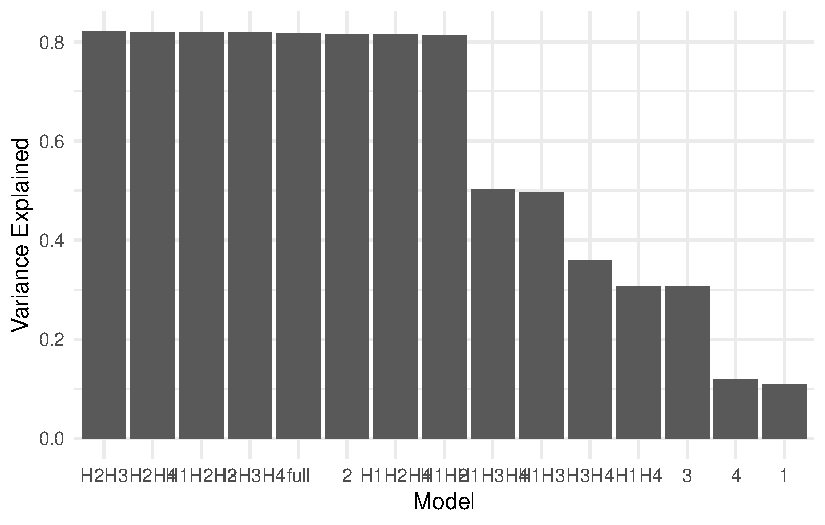
\includegraphics{MachineLearning_StaticPatterNN_Report_files/figure-pdf/var-part-ranger-performance-eval-1.pdf}

\subsubsection{Predictor importance / Recursive Feature
Selection}\label{predictor-importance-recursive-feature-selection}

\begin{Shaded}
\begin{Highlighting}[]
\DocumentationTok{\#\# Default summary function (rfFuncs)}
\NormalTok{rfFuncs }\OtherTok{\textless{}{-}} \FunctionTok{list}\NormalTok{(}
    \AttributeTok{summary =} 
    \ControlFlowTok{function}\NormalTok{ (data, }\AttributeTok{lev =} \ConstantTok{NULL}\NormalTok{, }\AttributeTok{model =} \ConstantTok{NULL}\NormalTok{) \{}
    \ControlFlowTok{if}\NormalTok{ (}\FunctionTok{is.character}\NormalTok{(data}\SpecialCharTok{$}\NormalTok{obs)) }
\NormalTok{        data}\SpecialCharTok{$}\NormalTok{obs }\OtherTok{\textless{}{-}} \FunctionTok{factor}\NormalTok{(data}\SpecialCharTok{$}\NormalTok{obs, }\AttributeTok{levels =}\NormalTok{ lev)}
    \FunctionTok{postResample}\NormalTok{(data[, }\StringTok{"pred"}\NormalTok{], data[, }\StringTok{"obs"}\NormalTok{])}
\NormalTok{    \},}
    
    \AttributeTok{fit =} 
    \ControlFlowTok{function}\NormalTok{ (x, y, first, last, ...) \{}
    \FunctionTok{loadNamespace}\NormalTok{(}\StringTok{"randomForest"}\NormalTok{)}
\NormalTok{    randomForest}\SpecialCharTok{::}\FunctionTok{randomForest}\NormalTok{(x, y, }\AttributeTok{importance =} \ConstantTok{TRUE}\NormalTok{, ...)}
\NormalTok{    \},}
    
    \AttributeTok{pred =} 
    \ControlFlowTok{function}\NormalTok{ (object, x) \{}
\NormalTok{    tmp }\OtherTok{\textless{}{-}} \FunctionTok{predict}\NormalTok{(object, x)}
    \ControlFlowTok{if}\NormalTok{ (}\FunctionTok{is.factor}\NormalTok{(object}\SpecialCharTok{$}\NormalTok{y)) \{}
\NormalTok{        out }\OtherTok{\textless{}{-}} \FunctionTok{cbind}\NormalTok{(}\FunctionTok{data.frame}\NormalTok{(}\AttributeTok{pred =}\NormalTok{ tmp), }\FunctionTok{as.data.frame}\NormalTok{(}\FunctionTok{predict}\NormalTok{(object, }
\NormalTok{            x, }\AttributeTok{type =} \StringTok{"prob"}\NormalTok{), }\AttributeTok{stringsAsFactors =} \ConstantTok{TRUE}\NormalTok{))\}}
    \ControlFlowTok{else}\NormalTok{ out }\OtherTok{\textless{}{-}}\NormalTok{ tmp}
\NormalTok{    out}
\NormalTok{    \},}
    
    \AttributeTok{rank =} 
    \ControlFlowTok{function}\NormalTok{ (object, x, y) \{}
\NormalTok{        vimp }\OtherTok{\textless{}{-}} \FunctionTok{varImp}\NormalTok{(object)}
        \ControlFlowTok{if}\NormalTok{ (}\FunctionTok{is.factor}\NormalTok{(y)) \{}
            \ControlFlowTok{if}\NormalTok{ (}\FunctionTok{all}\NormalTok{(}\FunctionTok{levels}\NormalTok{(y) }\SpecialCharTok{\%in\%} \FunctionTok{colnames}\NormalTok{(vimp))) \{}
\NormalTok{                avImp }\OtherTok{\textless{}{-}} \FunctionTok{apply}\NormalTok{(vimp[, }\FunctionTok{levels}\NormalTok{(y), }\AttributeTok{drop =} \ConstantTok{TRUE}\NormalTok{], }\DecValTok{1}\NormalTok{, mean)}
\NormalTok{                vimp}\SpecialCharTok{$}\NormalTok{Overall }\OtherTok{\textless{}{-}}\NormalTok{ avImp\}}
\NormalTok{                \}}
\NormalTok{        vimp }\OtherTok{\textless{}{-}}\NormalTok{ vimp[}\FunctionTok{order}\NormalTok{(vimp}\SpecialCharTok{$}\NormalTok{Overall, }\AttributeTok{decreasing =} \ConstantTok{TRUE}\NormalTok{), , drop }\OtherTok{=} \ConstantTok{FALSE}\NormalTok{]}
        \ControlFlowTok{if}\NormalTok{ (}\FunctionTok{ncol}\NormalTok{(x) }\SpecialCharTok{==} \DecValTok{1}\NormalTok{) \{}
\NormalTok{            vimp}\SpecialCharTok{$}\NormalTok{var }\OtherTok{\textless{}{-}} \FunctionTok{colnames}\NormalTok{(x)\}}
        \ControlFlowTok{else}\NormalTok{ vimp}\SpecialCharTok{$}\NormalTok{var }\OtherTok{\textless{}{-}} \FunctionTok{rownames}\NormalTok{(vimp)}
\NormalTok{        vimp}
\NormalTok{    \},}

    \AttributeTok{selectSize =} 
    \ControlFlowTok{function}\NormalTok{ (x, metric, maximize) \{}
\NormalTok{        best }\OtherTok{\textless{}{-}} \ControlFlowTok{if}\NormalTok{ (maximize) }
        \FunctionTok{which.max}\NormalTok{(x[, metric])}
        \ControlFlowTok{else} \FunctionTok{which.min}\NormalTok{(x[, metric])}
        \FunctionTok{min}\NormalTok{(x[best, }\StringTok{"Variables"}\NormalTok{])}
\NormalTok{    \},}

    \AttributeTok{selectVar =} 
    \ControlFlowTok{function}\NormalTok{ (y, size) \{}
\NormalTok{        finalImp }\OtherTok{\textless{}{-}} \FunctionTok{ddply}\NormalTok{(y[, }\FunctionTok{c}\NormalTok{(}\StringTok{"Overall"}\NormalTok{, }\StringTok{"var"}\NormalTok{)], .(var), }\ControlFlowTok{function}\NormalTok{(x) }\FunctionTok{mean}\NormalTok{(x}\SpecialCharTok{$}\NormalTok{Overall, }
        \AttributeTok{na.rm =} \ConstantTok{TRUE}\NormalTok{))}
        \FunctionTok{names}\NormalTok{(finalImp)[}\DecValTok{2}\NormalTok{] }\OtherTok{\textless{}{-}} \StringTok{"Overall"}
\NormalTok{        finalImp }\OtherTok{\textless{}{-}}\NormalTok{ finalImp[}\FunctionTok{order}\NormalTok{(finalImp}\SpecialCharTok{$}\NormalTok{Overall, }\AttributeTok{decreasing =} \ConstantTok{TRUE}\NormalTok{), ]}
        \FunctionTok{as.character}\NormalTok{(finalImp}\SpecialCharTok{$}\NormalTok{var[}\DecValTok{1}\SpecialCharTok{:}\NormalTok{size])}
\NormalTok{    \}}
\NormalTok{)}


\DocumentationTok{\#\# Custom summary function for randomForest (simplified)}
\NormalTok{rfRFE1 }\OtherTok{\textless{}{-}} \FunctionTok{list}\NormalTok{(}
    \AttributeTok{summary =}\NormalTok{ defaultSummary,}
    \AttributeTok{fit =} \ControlFlowTok{function}\NormalTok{(x, y, first, last, ...) \{}
        \FunctionTok{library}\NormalTok{(randomForest)}
        \FunctionTok{randomForest}\NormalTok{(x, y, }\AttributeTok{importance =}\NormalTok{ first, ...)}
\NormalTok{    \},}
    \AttributeTok{pred =} \ControlFlowTok{function}\NormalTok{(object, x) }\FunctionTok{predict}\NormalTok{(object, x),}
    \AttributeTok{rank =} \ControlFlowTok{function}\NormalTok{(object, x, y) \{}
\NormalTok{        vimp }\OtherTok{\textless{}{-}} \FunctionTok{varImp}\NormalTok{(object, }\AttributeTok{type =} \DecValTok{1}\NormalTok{, }\AttributeTok{scale =} \ConstantTok{TRUE}\NormalTok{)}
\NormalTok{        vimp }\OtherTok{\textless{}{-}}\NormalTok{ vimp[}\FunctionTok{order}\NormalTok{(vimp}\SpecialCharTok{$}\NormalTok{Overall, }\AttributeTok{decreasing =} \ConstantTok{TRUE}\NormalTok{), , drop }\OtherTok{=} \ConstantTok{FALSE}\NormalTok{]}
\NormalTok{        vimp}\SpecialCharTok{$}\NormalTok{var }\OtherTok{\textless{}{-}} \FunctionTok{rownames}\NormalTok{(vimp)}
\NormalTok{        vimp}
\NormalTok{    \},}
    \AttributeTok{selectSize =}\NormalTok{ pickSizeBest,}
    \AttributeTok{selectVar =}\NormalTok{ pickVars}
\NormalTok{)}


\DocumentationTok{\#\# Recursive feature selection:}
\FunctionTok{set.seed}\NormalTok{(}\DecValTok{42}\NormalTok{)}
\NormalTok{ctrl }\OtherTok{\textless{}{-}} \FunctionTok{rfeControl}\NormalTok{(}
    \AttributeTok{functions =}\NormalTok{ rfFuncs,}
    \AttributeTok{method =} \StringTok{"repeatedcv"}\NormalTok{,}
    \AttributeTok{number =} \DecValTok{10}\NormalTok{,}
    \AttributeTok{repeats =} \DecValTok{3}\NormalTok{,}
    \AttributeTok{returnResamp =} \StringTok{"all"}\NormalTok{, }\CommentTok{\# we need all resamples}
    \AttributeTok{verbose =} \ConstantTok{FALSE}\NormalTok{,}
    \AttributeTok{index =}\NormalTok{ indices,}
    \AttributeTok{saveDetails =} \ConstantTok{TRUE}\NormalTok{,}
    \AttributeTok{timingSamps =} \DecValTok{10}
\NormalTok{)}

\NormalTok{rank }\OtherTok{\textless{}{-}} \ControlFlowTok{function}\NormalTok{ (object, x, y)\{}
\NormalTok{    vimp }\OtherTok{\textless{}{-}} \FunctionTok{varImp}\NormalTok{(object, }\AttributeTok{type =} \DecValTok{1}\NormalTok{, }\AttributeTok{scale =} \ConstantTok{TRUE}\NormalTok{)}
    \ControlFlowTok{if}\NormalTok{ (}\FunctionTok{is.factor}\NormalTok{(y)) \{}
        \ControlFlowTok{if}\NormalTok{ (}\FunctionTok{all}\NormalTok{(}\FunctionTok{levels}\NormalTok{(y) }\SpecialCharTok{\%in\%} \FunctionTok{colnames}\NormalTok{(vimp))) \{}
\NormalTok{            avImp }\OtherTok{\textless{}{-}} \FunctionTok{apply}\NormalTok{(vimp[, }\FunctionTok{levels}\NormalTok{(y), }\AttributeTok{drop =} \ConstantTok{TRUE}\NormalTok{], }\DecValTok{1}\NormalTok{, }
\NormalTok{                mean)}
\NormalTok{            vimp}\SpecialCharTok{$}\NormalTok{Overall }\OtherTok{\textless{}{-}}\NormalTok{ avImp}
\NormalTok{        \}}
\NormalTok{    \}}
\NormalTok{    vimp }\OtherTok{\textless{}{-}}\NormalTok{ vimp[}\FunctionTok{order}\NormalTok{(vimp}\SpecialCharTok{$}\NormalTok{Overall, }\AttributeTok{decreasing =} \ConstantTok{TRUE}\NormalTok{), , drop }\OtherTok{=} \ConstantTok{FALSE}\NormalTok{]}
    \ControlFlowTok{if}\NormalTok{ (}\FunctionTok{ncol}\NormalTok{(x) }\SpecialCharTok{==} \DecValTok{1}\NormalTok{) \{}
\NormalTok{        vimp}\SpecialCharTok{$}\NormalTok{var }\OtherTok{\textless{}{-}} \FunctionTok{colnames}\NormalTok{(x)}
\NormalTok{    \}}
    \ControlFlowTok{else}\NormalTok{ vimp}\SpecialCharTok{$}\NormalTok{var }\OtherTok{\textless{}{-}} \FunctionTok{rownames}\NormalTok{(vimp)}
\NormalTok{    vimp}
\NormalTok{\}}
\NormalTok{ctrl}\SpecialCharTok{$}\NormalTok{functions}\SpecialCharTok{$}\NormalTok{rank }\OtherTok{\textless{}{-}}\NormalTok{ rank}

\DocumentationTok{\#\# Variable importance}
\FunctionTok{set.seed}\NormalTok{(}\DecValTok{42}\NormalTok{)}
\NormalTok{ctrl2 }\OtherTok{\textless{}{-}} \FunctionTok{rfeControl}\NormalTok{(}
    \AttributeTok{functions =}\NormalTok{ rfRFE1,}
    \AttributeTok{method =} \StringTok{"repeatedcv"}\NormalTok{,}
    \AttributeTok{number =} \DecValTok{10}\NormalTok{,}
    \AttributeTok{repeats =} \DecValTok{3}\NormalTok{,}
    \AttributeTok{returnResamp =} \StringTok{"all"}\NormalTok{, }\CommentTok{\# we need all resamples}
    \AttributeTok{verbose =} \ConstantTok{FALSE}\NormalTok{,}
    \AttributeTok{index =}\NormalTok{ indices,}
    \AttributeTok{saveDetails =} \ConstantTok{TRUE}\NormalTok{,}
    \AttributeTok{timingSamps =} \DecValTok{10}
\NormalTok{)}



\FunctionTok{set.seed}\NormalTok{(}\DecValTok{42}\NormalTok{)}
\NormalTok{subsets }\OtherTok{\textless{}{-}} \FunctionTok{c}\NormalTok{(}\DecValTok{1}\SpecialCharTok{:}\DecValTok{50}\NormalTok{)}

\NormalTok{x }\OtherTok{\textless{}{-}}\NormalTok{ dat\_train }\SpecialCharTok{\%\textgreater{}\%} \FunctionTok{select}\NormalTok{(}\SpecialCharTok{{-}}\NormalTok{Jaccard)}
\NormalTok{y }\OtherTok{\textless{}{-}}\NormalTok{ dat\_train }\SpecialCharTok{\%\textgreater{}\%} \FunctionTok{pull}\NormalTok{(Jaccard)}


\CommentTok{\# Empty list of lists that will be filled with each iteration of the loop (total = 10 iterations}
\NormalTok{saved\_profiles }\OtherTok{\textless{}{-}} \FunctionTok{replicate}\NormalTok{(}\DecValTok{10}\NormalTok{, }\FunctionTok{list}\NormalTok{())}
\NormalTok{tictoc}\SpecialCharTok{::}\FunctionTok{tic}\NormalTok{()}
\ControlFlowTok{for}\NormalTok{ (i }\ControlFlowTok{in} \DecValTok{1}\SpecialCharTok{:}\DecValTok{10}\NormalTok{)\{}


\DocumentationTok{\#\# First run:}
\NormalTok{rfProfile }\OtherTok{\textless{}{-}} \FunctionTok{rfe}\NormalTok{(x, y, }\AttributeTok{sizes =}\NormalTok{ subsets, }\AttributeTok{rfeControl =}\NormalTok{ ctrl, }\AttributeTok{ntrees =} \DecValTok{5000}\NormalTok{)}
\NormalTok{rfProfile}

\CommentTok{\# Most important predictors:}
\NormalTok{rfProfile}\SpecialCharTok{$}\NormalTok{fit}\SpecialCharTok{$}\NormalTok{importance }\SpecialCharTok{\%\textgreater{}\%} 
    \FunctionTok{round}\NormalTok{(}\DecValTok{3}\NormalTok{) }\SpecialCharTok{\%\textgreater{}\%} 
    \FunctionTok{as.data.frame}\NormalTok{() }\SpecialCharTok{\%\textgreater{}\%}
    \FunctionTok{select}\NormalTok{(}\StringTok{"\%IncMSE"}\NormalTok{) }\SpecialCharTok{\%\textgreater{}\%}
    \FunctionTok{arrange}\NormalTok{(}\FunctionTok{desc}\NormalTok{(.))}
\NormalTok{imp1 }\OtherTok{\textless{}{-}} \FunctionTok{varImp}\NormalTok{(rfProfile) }\CommentTok{\# overall importance (mean across resamples)}
\DocumentationTok{\#\# This one selects 35 variables}
\DocumentationTok{\#\# Second run: selects 32 variables}


\DocumentationTok{\#\# Second run:}
\NormalTok{rfProfile2 }\OtherTok{\textless{}{-}} \FunctionTok{rfe}\NormalTok{(x, y, }\AttributeTok{sizes =}\NormalTok{ subsets, }\AttributeTok{rfeControl =}\NormalTok{ ctrl2, }\AttributeTok{ntrees =} \DecValTok{5000}\NormalTok{)}
\NormalTok{rfProfile2}\SpecialCharTok{$}\NormalTok{fit}\SpecialCharTok{$}\NormalTok{importance }\SpecialCharTok{\%\textgreater{}\%}
    \FunctionTok{round}\NormalTok{(}\DecValTok{3}\NormalTok{) }\SpecialCharTok{\%\textgreater{}\%} 
    \FunctionTok{as.data.frame}\NormalTok{() }\SpecialCharTok{\%\textgreater{}\%}
    \CommentTok{\#select("\%IncMSE") \%\textgreater{}\%}
    \FunctionTok{arrange}\NormalTok{(}\FunctionTok{desc}\NormalTok{(.))}

\NormalTok{imp2 }\OtherTok{\textless{}{-}} \FunctionTok{varImp}\NormalTok{(rfProfile2)}


\DocumentationTok{\#\# This one selects only 20 variables}
\DocumentationTok{\#\# Second run: selects 31 variables}

\DocumentationTok{\#\# Comparison between both models:}
\FunctionTok{merge}\NormalTok{(imp1,imp2, }\AttributeTok{by =} \StringTok{"row.names"}\NormalTok{, }\AttributeTok{all =}\NormalTok{ T) }\SpecialCharTok{\%\textgreater{}\%} 
    \FunctionTok{mutate\_if}\NormalTok{(is.numeric, round, }\AttributeTok{digits =} \DecValTok{3}\NormalTok{) }\SpecialCharTok{\%\textgreater{}\%}
    \FunctionTok{as.data.frame}\NormalTok{() }\SpecialCharTok{\%\textgreater{}\%}
    \FunctionTok{arrange}\NormalTok{(}\FunctionTok{desc}\NormalTok{(Overall.x))}

\NormalTok{saved\_profiles[[i]] }\OtherTok{\textless{}{-}} \FunctionTok{list}\NormalTok{(rfProfile, rfProfile2)}
\NormalTok{\}}

\NormalTok{tictoc}\SpecialCharTok{::}\FunctionTok{toc}\NormalTok{()}

\CommentTok{\# save.image("data/varPart\_rfe.RData")}
\end{Highlighting}
\end{Shaded}

\begin{Shaded}
\begin{Highlighting}[]
\NormalTok{results }\OtherTok{\textless{}{-}} \FunctionTok{replicate}\NormalTok{(}\DecValTok{10}\NormalTok{, }\FunctionTok{list}\NormalTok{())}
\ControlFlowTok{for}\NormalTok{(i }\ControlFlowTok{in} \FunctionTok{seq\_along}\NormalTok{(}\DecValTok{1}\SpecialCharTok{:}\FunctionTok{length}\NormalTok{(saved\_profiles)))\{}
    \ControlFlowTok{for}\NormalTok{ (y }\ControlFlowTok{in} \FunctionTok{seq\_along}\NormalTok{(}\DecValTok{1}\SpecialCharTok{:}\FunctionTok{length}\NormalTok{(saved\_profiles[[i]])))\{}
\NormalTok{        resamp\_res }\OtherTok{\textless{}{-}}\NormalTok{ saved\_profiles[[i]][[y]]}
\NormalTok{        res }\OtherTok{\textless{}{-}} \FunctionTok{slice\_min}\NormalTok{(resamp\_res}\SpecialCharTok{$}\NormalTok{results, RMSE)}
\NormalTok{        results[[i]][[y]] }\OtherTok{\textless{}{-}}\NormalTok{ res}
        
\NormalTok{    \}}
\NormalTok{\}}

\NormalTok{rfe\_res }\OtherTok{\textless{}{-}} \FunctionTok{do.call}\NormalTok{(rbind, }\FunctionTok{unlist}\NormalTok{(results, }\AttributeTok{recursive =} \ConstantTok{FALSE}\NormalTok{))}
\NormalTok{rfe\_res}\SpecialCharTok{$}\NormalTok{model }\OtherTok{\textless{}{-}} \FunctionTok{rep}\NormalTok{(}\FunctionTok{c}\NormalTok{(}\StringTok{"default"}\NormalTok{, }\StringTok{"simple"}\NormalTok{), }\DecValTok{10}\NormalTok{)}
\FunctionTok{ggplot}\NormalTok{(}\AttributeTok{data =}\NormalTok{ rfe\_res, }\FunctionTok{aes}\NormalTok{(}\AttributeTok{x =}\NormalTok{ model, }\AttributeTok{y =}\NormalTok{ Variables)) }\SpecialCharTok{+}
    \FunctionTok{geom\_boxplot}\NormalTok{() }\SpecialCharTok{+}
    \FunctionTok{geom\_point}\NormalTok{(}\AttributeTok{data =}\NormalTok{ rfe\_res }\SpecialCharTok{\%\textgreater{}\%} \FunctionTok{group\_by}\NormalTok{(model) }\SpecialCharTok{\%\textgreater{}\%} \FunctionTok{summarize}\NormalTok{(}\AttributeTok{mean\_Variables =} \FunctionTok{mean}\NormalTok{(Variables)), }
    \FunctionTok{aes}\NormalTok{(}\AttributeTok{x =}\NormalTok{ model, }\AttributeTok{y =}\NormalTok{ mean\_Variables), }\AttributeTok{color =} \StringTok{"red"}\NormalTok{) }\SpecialCharTok{+}
    \FunctionTok{theme\_bw}\NormalTok{()}
\end{Highlighting}
\end{Shaded}

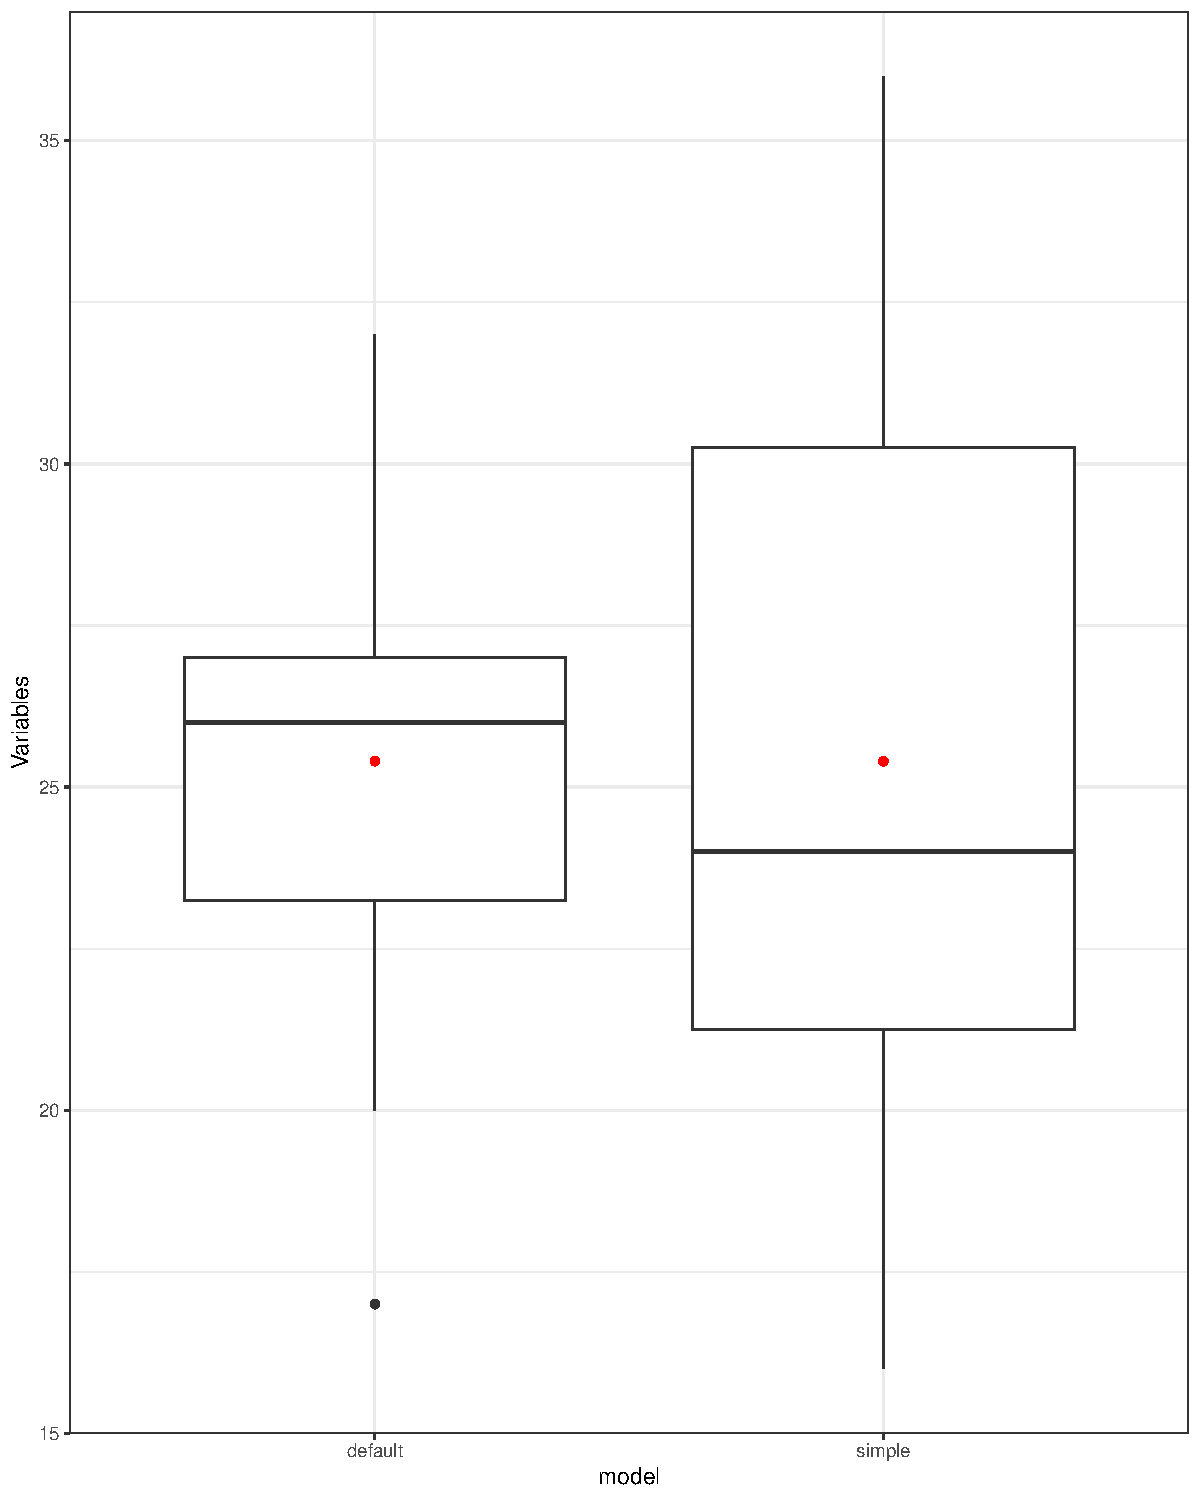
\includegraphics{MachineLearning_StaticPatterNN_Report_files/figure-pdf/rfe-results-1.pdf}

\begin{Shaded}
\begin{Highlighting}[]
\NormalTok{rfe\_res }\SpecialCharTok{\%\textgreater{}\%} \FunctionTok{group\_by}\NormalTok{(model) }\SpecialCharTok{\%\textgreater{}\%} \FunctionTok{summarize}\NormalTok{(}\AttributeTok{mean\_Variables =} \FunctionTok{mean}\NormalTok{(Variables)) }\CommentTok{\# 25.4 for both}
\end{Highlighting}
\end{Shaded}

\begin{verbatim}
# A tibble: 2 x 2
  model   mean_Variables
  <chr>            <dbl>
1 default           25.4
2 simple            25.4
\end{verbatim}

\begin{Shaded}
\begin{Highlighting}[]
\NormalTok{rfe\_res }\SpecialCharTok{\%\textgreater{}\%} \FunctionTok{group\_by}\NormalTok{(model) }\SpecialCharTok{\%\textgreater{}\%} \FunctionTok{summarize}\NormalTok{(}\AttributeTok{median\_Variables =} \FunctionTok{median}\NormalTok{(Variables)) }\CommentTok{\# 26 for default, 24 for simple. Let\textquotesingle{}s go with the results for the default model: 26.}
\end{Highlighting}
\end{Shaded}

\begin{verbatim}
# A tibble: 2 x 2
  model   median_Variables
  <chr>              <dbl>
1 default               26
2 simple                24
\end{verbatim}

\begin{Shaded}
\begin{Highlighting}[]
\NormalTok{saved\_res2 }\OtherTok{\textless{}{-}} \FunctionTok{unlist}\NormalTok{(saved\_profiles, }\AttributeTok{recursive =} \ConstantTok{FALSE}\NormalTok{)}
\NormalTok{saved\_res3 }\OtherTok{\textless{}{-}}\NormalTok{ saved\_res2[}\FunctionTok{c}\NormalTok{(}\FunctionTok{seq}\NormalTok{(}\AttributeTok{from =} \DecValTok{1}\NormalTok{, }\AttributeTok{to =} \DecValTok{20}\NormalTok{, }\AttributeTok{by =} \DecValTok{2}\NormalTok{))] }\CommentTok{\# keep only default models}

\NormalTok{res\_top\_vars }\OtherTok{\textless{}{-}} \FunctionTok{list}\NormalTok{()}
\ControlFlowTok{for}\NormalTok{(i }\ControlFlowTok{in} \FunctionTok{seq\_along}\NormalTok{(saved\_res3))\{}

\NormalTok{res\_top\_vars[[i]] }\OtherTok{\textless{}{-}} \FunctionTok{data.frame}\NormalTok{(}
    \AttributeTok{var =} \FunctionTok{row.names}\NormalTok{(}\FunctionTok{varImp}\NormalTok{(saved\_res3[[i]], }\AttributeTok{scale =}\NormalTok{ T)),}
    \AttributeTok{Imp =} \FunctionTok{varImp}\NormalTok{(saved\_res3[[i]])}\SpecialCharTok{$}\NormalTok{Overall,}
    \AttributeTok{include =} \FunctionTok{c}\NormalTok{(}\FunctionTok{rep\_len}\NormalTok{(}\DecValTok{1}\NormalTok{, }\FunctionTok{as.numeric}\NormalTok{(saved\_res3[[i]]}\SpecialCharTok{$}\NormalTok{bestSubset)), }
                \FunctionTok{rep\_len}\NormalTok{(}\DecValTok{0}\NormalTok{,  }
                \FunctionTok{length}\NormalTok{(}\FunctionTok{row.names}\NormalTok{(}\FunctionTok{varImp}\NormalTok{(saved\_res3[[i]], }\AttributeTok{scale =}\NormalTok{ T)))}\SpecialCharTok{{-}}\FunctionTok{as.numeric}\NormalTok{(saved\_res3[[i]]}\SpecialCharTok{$}\NormalTok{bestSubset))}
\NormalTok{            ),}
    \AttributeTok{model =}\NormalTok{ i}
\NormalTok{        )}
\NormalTok{\}}

\NormalTok{res\_top\_vars\_df }\OtherTok{\textless{}{-}} \FunctionTok{do.call}\NormalTok{(rbind, res\_top\_vars)}



\DocumentationTok{\#\#\# Plot =====}

\CommentTok{\# Calculate the maximum count of resamples for scaling}
\NormalTok{max\_count }\OtherTok{\textless{}{-}}\NormalTok{ res\_top\_vars\_df }\SpecialCharTok{\%\textgreater{}\%} \FunctionTok{count}\NormalTok{(var) }\SpecialCharTok{\%\textgreater{}\%} \FunctionTok{pull}\NormalTok{(n) }\SpecialCharTok{\%\textgreater{}\%} \FunctionTok{max}\NormalTok{()}

\FunctionTok{ggplot}\NormalTok{(}\AttributeTok{data =}\NormalTok{ res\_top\_vars\_df) }\SpecialCharTok{+}
  \CommentTok{\# Background rectangles}
  \FunctionTok{geom\_rect}\NormalTok{(}\FunctionTok{aes}\NormalTok{(}\AttributeTok{xmin =} \SpecialCharTok{{-}}\ConstantTok{Inf}\NormalTok{, }\AttributeTok{xmax =} \ConstantTok{Inf}\NormalTok{, }\AttributeTok{ymin =} \SpecialCharTok{{-}}\ConstantTok{Inf}\NormalTok{, }\AttributeTok{ymax =} \FloatTok{10.5}\NormalTok{), }
            \AttributeTok{fill =} \StringTok{"lightgray"}\NormalTok{, }\AttributeTok{alpha =} \FloatTok{0.9}\NormalTok{) }\SpecialCharTok{+}
  \CommentTok{\# Box plot}
  \FunctionTok{geom\_boxplot}\NormalTok{(}\FunctionTok{aes}\NormalTok{(}\AttributeTok{y =} \FunctionTok{reorder}\NormalTok{(var, Imp), }\AttributeTok{x =}\NormalTok{ Imp)) }\SpecialCharTok{+}
  \CommentTok{\# Bar plot scaled to the secondary axis}
  \FunctionTok{geom\_bar}\NormalTok{(}\FunctionTok{aes}\NormalTok{(}\AttributeTok{y =} \FunctionTok{reorder}\NormalTok{(var, Imp), }\AttributeTok{x =} \FunctionTok{after\_stat}\NormalTok{(count) }\SpecialCharTok{/}\NormalTok{ max\_count }\SpecialCharTok{*} \FunctionTok{max}\NormalTok{(res\_top\_vars\_df}\SpecialCharTok{$}\NormalTok{Imp), }
               \AttributeTok{fill =} \FunctionTok{factor}\NormalTok{(include)), }\AttributeTok{stat =} \StringTok{"count"}\NormalTok{,  }\AttributeTok{alpha =} \FloatTok{0.3}\NormalTok{) }\SpecialCharTok{+}
  \CommentTok{\# Horizontal line}
  \FunctionTok{geom\_hline}\NormalTok{(}\AttributeTok{yintercept =} \FloatTok{10.5}\NormalTok{) }\SpecialCharTok{+}
  \CommentTok{\# Secondary axis that stretches through the entire range}
  \FunctionTok{scale\_x\_continuous}\NormalTok{(}\AttributeTok{sec.axis =} \FunctionTok{sec\_axis}\NormalTok{(}\SpecialCharTok{\textasciitilde{}}\NormalTok{ . }\SpecialCharTok{*}\NormalTok{ max\_count }\SpecialCharTok{/} \FunctionTok{max}\NormalTok{(res\_top\_vars\_df}\SpecialCharTok{$}\NormalTok{Imp), }
                                         \AttributeTok{name =} \StringTok{"Count Resamples (Secondary Axis)"}\NormalTok{)) }\SpecialCharTok{+}
  \CommentTok{\# Scale and theme}
  \FunctionTok{scale\_fill\_manual}\NormalTok{(}\AttributeTok{values =} \FunctionTok{c}\NormalTok{(}\StringTok{"\#D55E00"}\NormalTok{, }\StringTok{"\#009E73"}\NormalTok{)) }\SpecialCharTok{+}
  \FunctionTok{theme\_bw}\NormalTok{() }\SpecialCharTok{+}
  \FunctionTok{theme}\NormalTok{(}\AttributeTok{legend.position =} \StringTok{"right"}\NormalTok{) }\SpecialCharTok{+}
  \FunctionTok{labs}\NormalTok{(}\AttributeTok{title =} \StringTok{"Top Variables by Importance"}\NormalTok{, }\AttributeTok{x =} \StringTok{"Importance"}\NormalTok{, }\AttributeTok{y =} \StringTok{"Variable"}\NormalTok{)}
\end{Highlighting}
\end{Shaded}

\begin{verbatim}
Warning in geom_rect(aes(xmin = -Inf, xmax = Inf, ymin = -Inf, ymax = 10.5), : All aesthetics have length 1, but the data has 313 rows.
i Please consider using `annotate()` or provide this layer with data containing
  a single row.
\end{verbatim}

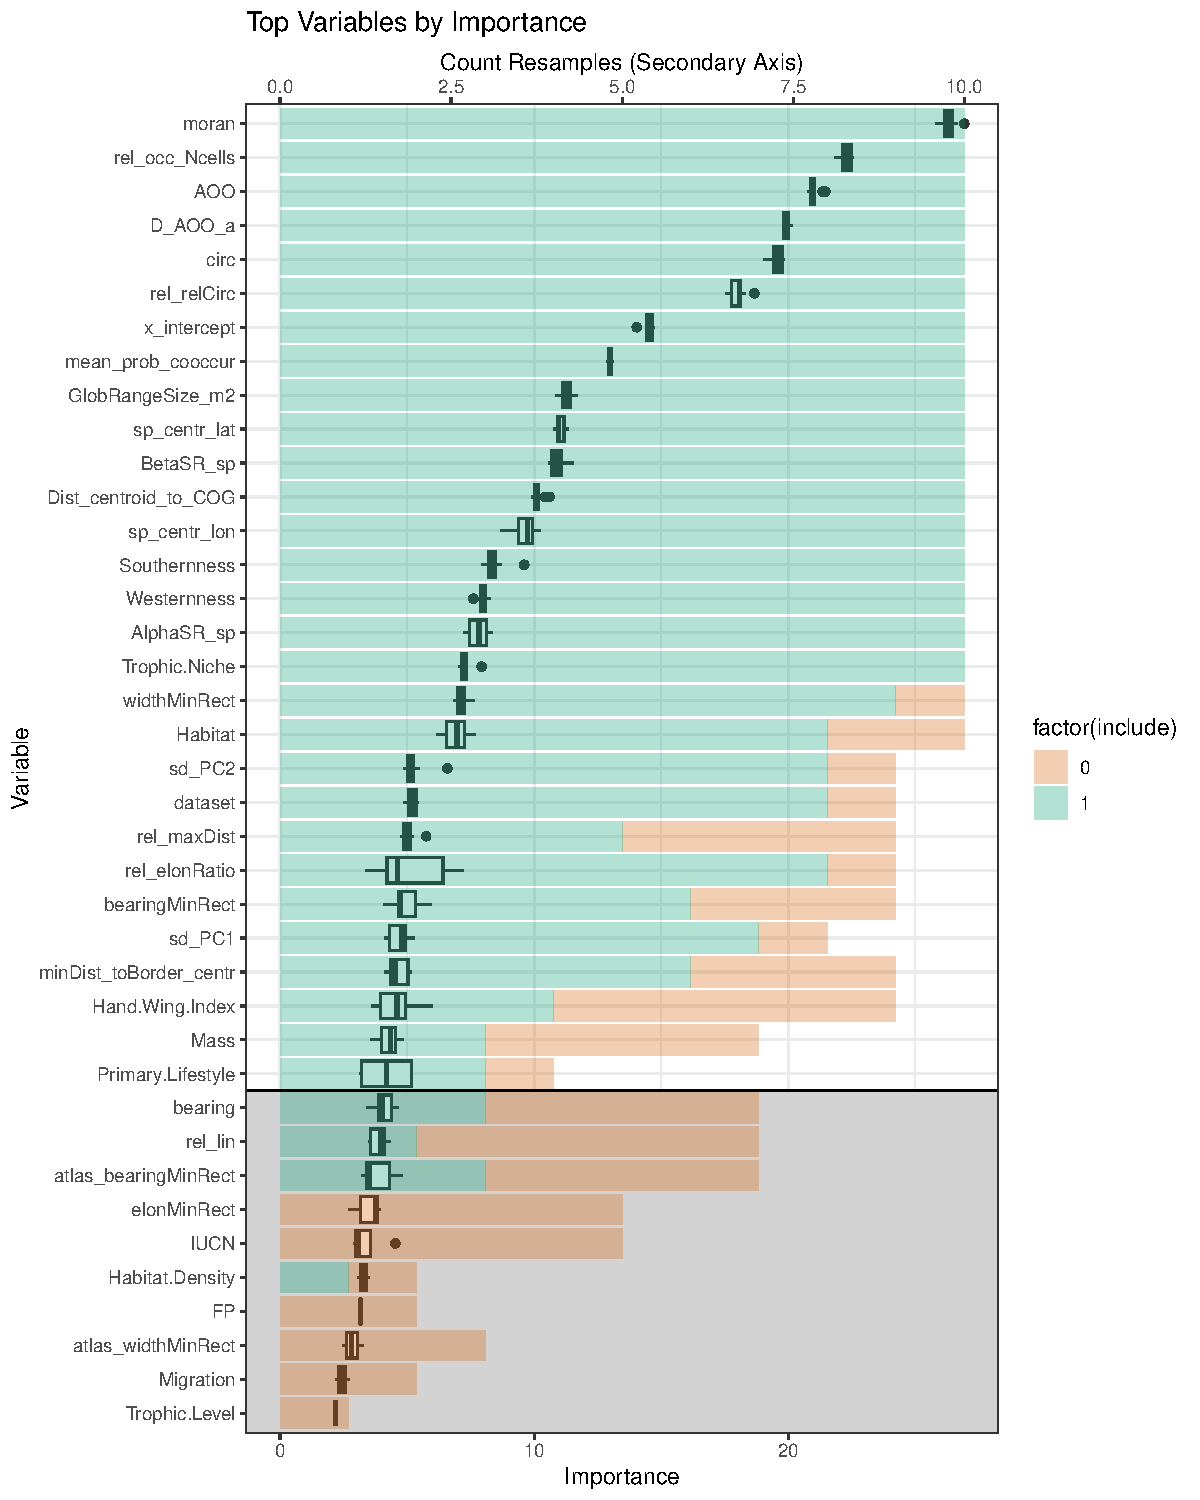
\includegraphics{MachineLearning_StaticPatterNN_Report_files/figure-pdf/rfe-results-2.pdf}

\subsubsection{Individual models}\label{individual-models}

\paragraph{Hyperparameter tuning}\label{hyperparameter-tuning}

\begin{Shaded}
\begin{Highlighting}[]
\CommentTok{\# Define training control ==========================================================}
\NormalTok{trainControl }\OtherTok{\textless{}{-}} \FunctionTok{trainControl}\NormalTok{(}
    \AttributeTok{method =} \StringTok{"repeatedcv"}\NormalTok{,}
    \AttributeTok{number =} \DecValTok{10}\NormalTok{,}
    \AttributeTok{repeats =} \DecValTok{3}\NormalTok{,}
    \AttributeTok{savePredictions =} \StringTok{"final"}\NormalTok{,}
    \AttributeTok{returnResamp =} \StringTok{"all"}\NormalTok{,}
    \AttributeTok{verboseIter =} \ConstantTok{FALSE}\NormalTok{,}
    \AttributeTok{index =}\NormalTok{ indices)}

\DocumentationTok{\#\# Train ranger model ==========================================================}
\CommentTok{\# set.seed(42)}
\CommentTok{\# tictoc::tic("ranger")}
\CommentTok{\# rangerModel\_t \textless{}{-} train(}
\CommentTok{\#     Jaccard \textasciitilde{} .,}
\CommentTok{\#     data = dat\_train,}
\CommentTok{\#     method = "ranger",}
\CommentTok{\#     trControl = trainControl,}
\CommentTok{\#     importance = "permutation",}
\CommentTok{\#     scale.permutation.importance = TRUE,}
\CommentTok{\#     num.trees = 5000,}
\CommentTok{\#     respect.unordered.factors = TRUE,}
\CommentTok{\#     oob.error = TRUE,}
\CommentTok{\#     tuneLength = 20)}
\CommentTok{\# saveRDS(rangerModel\_t, "./data/rangerModel\_all.rds")}
\CommentTok{\# tictoc::toc()}
\NormalTok{rangerModel\_t }\OtherTok{\textless{}{-}} \FunctionTok{readRDS}\NormalTok{(}\StringTok{"./data/rangerModel\_all.rds"}\NormalTok{)}

\DocumentationTok{\#\#\# Model results:}
\NormalTok{p\_rangerModel }\OtherTok{\textless{}{-}} \FunctionTok{plot}\NormalTok{(rangerModel\_t)}
\NormalTok{p\_rangerModel}
\end{Highlighting}
\end{Shaded}

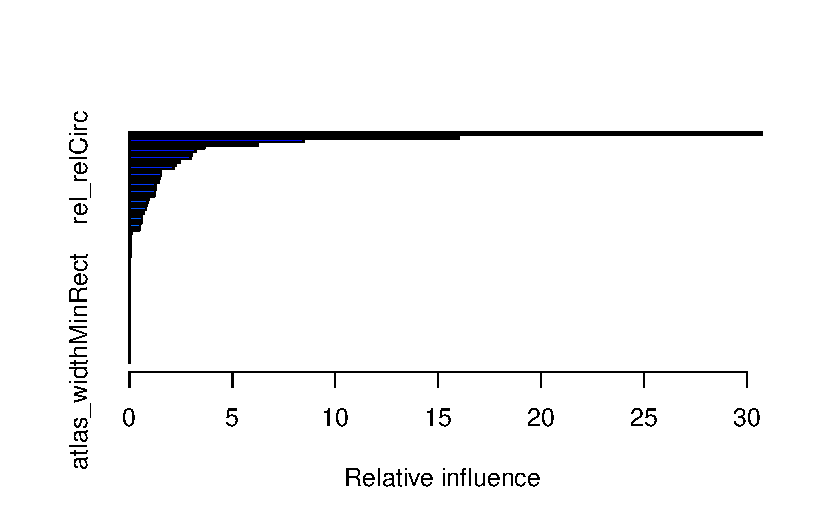
\includegraphics{MachineLearning_StaticPatterNN_Report_files/figure-pdf/hyperparameter-tuning-1.pdf}

\begin{Shaded}
\begin{Highlighting}[]
\NormalTok{rangerModel\_t}\SpecialCharTok{$}\NormalTok{finalModel}
\end{Highlighting}
\end{Shaded}

\begin{verbatim}
Ranger result

Call:
 ranger::ranger(dependent.variable.name = ".outcome", data = x,      mtry = min(param$mtry, ncol(x)), min.node.size = param$min.node.size,      splitrule = as.character(param$splitrule), write.forest = TRUE,      probability = classProbs, ...) 

Type:                             Regression 
Number of trees:                  5000 
Sample size:                      826 
Number of independent variables:  68 
Mtry:                             57 
Target node size:                 5 
Variable importance mode:         permutation 
Splitrule:                        extratrees 
Number of random splits:          1 
OOB prediction error (MSE):       0.0127173 
R squared (OOB):                  0.8409138 
\end{verbatim}

\begin{Shaded}
\begin{Highlighting}[]
\DocumentationTok{\#\# Train xgbTree model ==========================================================}
\NormalTok{xgb\_grid }\OtherTok{\textless{}{-}} \FunctionTok{expand.grid}\NormalTok{(}
  \AttributeTok{nrounds =} \FunctionTok{c}\NormalTok{(}\DecValTok{1000}\NormalTok{),}
  \AttributeTok{eta =} \FunctionTok{c}\NormalTok{(}\FloatTok{0.1}\NormalTok{, }\FloatTok{0.3}\NormalTok{),}
  \AttributeTok{max\_depth =} \FunctionTok{c}\NormalTok{(}\DecValTok{2}\NormalTok{,}\DecValTok{3}\NormalTok{, }\DecValTok{5}\NormalTok{),}
  \AttributeTok{gamma =} \FunctionTok{c}\NormalTok{(}\DecValTok{0}\NormalTok{, }\FloatTok{0.01}\NormalTok{, }\FloatTok{0.1}\NormalTok{),}
  \AttributeTok{colsample\_bytree =} \FloatTok{0.6}\NormalTok{,}
  \AttributeTok{min\_child\_weight =} \DecValTok{1}\NormalTok{,}
  \AttributeTok{subsample =} \FunctionTok{c}\NormalTok{(}\FloatTok{0.75}\NormalTok{, }\DecValTok{1}\NormalTok{))}

\CommentTok{\# tictoc::tic("xgb")}
\CommentTok{\# set.seed(42)}
\CommentTok{\# xgbModel\_t \textless{}{-} train(}
\CommentTok{\#     Jaccard \textasciitilde{} .,}
\CommentTok{\#     data = dat\_train,}
\CommentTok{\#     method = "xgbTree",}
\CommentTok{\#     trControl = trainControl,}
\CommentTok{\#     tuneGrid = xgb\_grid)}
\CommentTok{\# tictoc::toc()}
\CommentTok{\# saveRDS(xgbModel\_t, "./data/xgbModel\_all\_TLCUSTOM.rds")}

\NormalTok{xgbModel\_t }\OtherTok{\textless{}{-}} \FunctionTok{readRDS}\NormalTok{(}\StringTok{"./data/xgbModel\_all\_TL3.rds"}\NormalTok{)}

\DocumentationTok{\#\#\# Model results:}
\NormalTok{p\_xgbModel }\OtherTok{\textless{}{-}} \FunctionTok{plot}\NormalTok{(xgbModel\_t)}
\NormalTok{p\_xgbModel}
\end{Highlighting}
\end{Shaded}

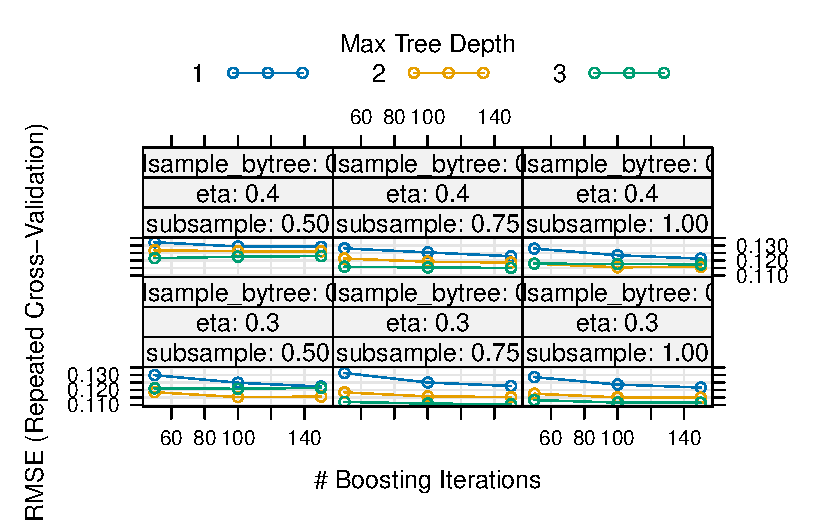
\includegraphics{MachineLearning_StaticPatterNN_Report_files/figure-pdf/hyperparameter-tuning-2.pdf}

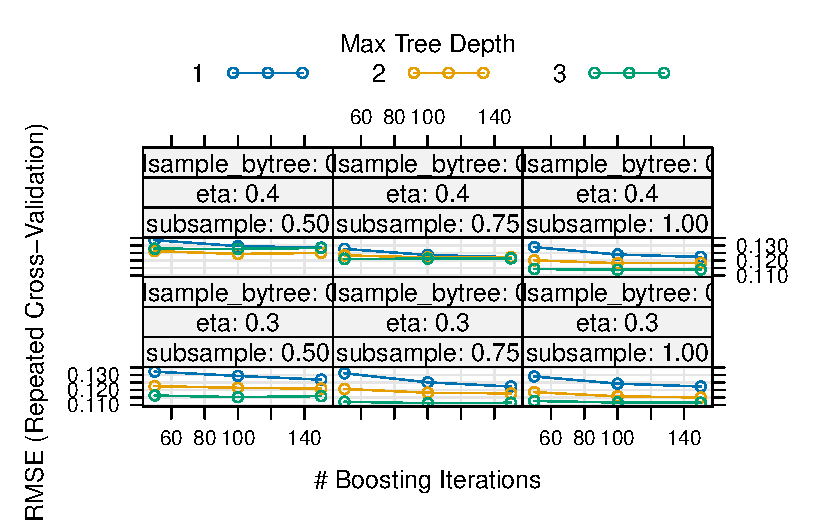
\includegraphics{MachineLearning_StaticPatterNN_Report_files/figure-pdf/hyperparameter-tuning-3.pdf}

\begin{Shaded}
\begin{Highlighting}[]
\FunctionTok{slice\_min}\NormalTok{(xgbModel\_t}\SpecialCharTok{$}\NormalTok{results, RMSE)}
\end{Highlighting}
\end{Shaded}

\begin{verbatim}
  eta max_depth gamma colsample_bytree min_child_weight subsample nrounds
1 0.3         3     0              0.6                1      0.75     150
       RMSE  Rsquared        MAE     RMSESD RsquaredSD       MAESD
1 0.1104851 0.8475537 0.07536493 0.01168408 0.03214512 0.005682521
\end{verbatim}

\begin{Shaded}
\begin{Highlighting}[]
\FunctionTok{slice\_max}\NormalTok{(xgbModel\_t}\SpecialCharTok{$}\NormalTok{results, Rsquared)}
\end{Highlighting}
\end{Shaded}

\begin{verbatim}
  eta max_depth gamma colsample_bytree min_child_weight subsample nrounds
1 0.3         3     0              0.6                1      0.75     150
       RMSE  Rsquared        MAE     RMSESD RsquaredSD       MAESD
1 0.1104851 0.8475537 0.07536493 0.01168408 0.03214512 0.005682521
\end{verbatim}

\begin{Shaded}
\begin{Highlighting}[]
\DocumentationTok{\#\# Train gbm model ==========================================================}
\CommentTok{\# set.seed(42)}
\CommentTok{\# tictoc::tic("gbm")}
\CommentTok{\# gbmModel\_t \textless{}{-} train(}
\CommentTok{\#     Jaccard \textasciitilde{} .,}
\CommentTok{\#     data = dat\_train,}
\CommentTok{\#     method = "gbm",}
\CommentTok{\#     trControl = trainControl,}
\CommentTok{\#     tuneLength= 20,}
\CommentTok{\#     verbose = FALSE)}
\CommentTok{\# saveRDS(gbmModel\_t, "./data/gbmModel\_all.rds")}
\CommentTok{\# tictoc::toc()}
\NormalTok{gbmModel\_t }\OtherTok{\textless{}{-}} \FunctionTok{readRDS}\NormalTok{(}\StringTok{"./data/gbmModel\_all.rds"}\NormalTok{)}

\DocumentationTok{\#\#\# Model results:}
\FunctionTok{summary.gbm}\NormalTok{(gbmModel\_t}\SpecialCharTok{$}\NormalTok{finalModel)}
\end{Highlighting}
\end{Shaded}

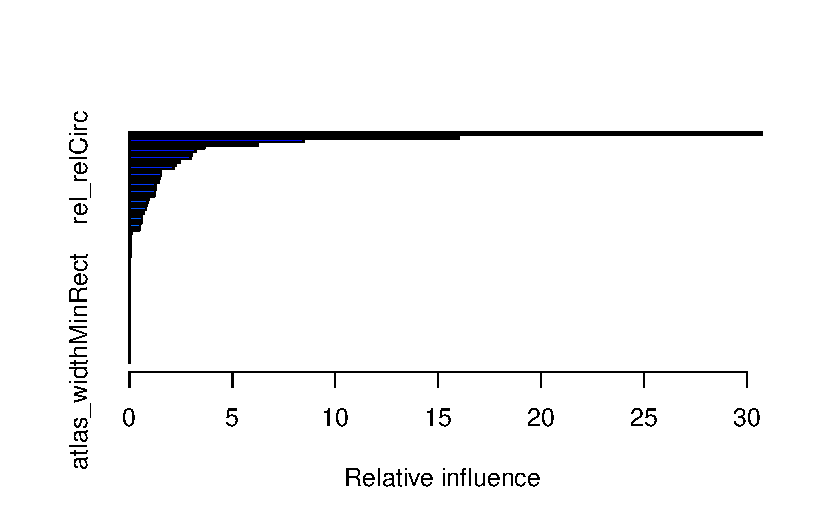
\includegraphics{MachineLearning_StaticPatterNN_Report_files/figure-pdf/hyperparameter-tuning-4.pdf}

\begin{verbatim}
                                                                  var
AOO                                                               AOO
rel_occ_Ncells                                         rel_occ_Ncells
moran                                                           moran
D_AOO_a                                                       D_AOO_a
circ                                                             circ
x_intercept                                               x_intercept
AlphaSR_sp                                                 AlphaSR_sp
BetaSR_sp                                                   BetaSR_sp
GlobRangeSize_m2                                     GlobRangeSize_m2
mean_prob_cooccur                                   mean_prob_cooccur
rel_relCirc                                               rel_relCirc
widthMinRect                                             widthMinRect
rel_maxDist                                               rel_maxDist
Southernness                                             Southernness
sp_centr_lat                                             sp_centr_lat
Westernness                                               Westernness
minDist_toBorder_centr                         minDist_toBorder_centr
Hand.Wing.Index                                       Hand.Wing.Index
sp_centr_lon                                             sp_centr_lon
Dist_centroid_to_COG                             Dist_centroid_to_COG
rel_elonRatio                                           rel_elonRatio
elonMinRect                                               elonMinRect
bearingMinRect                                         bearingMinRect
Mass                                                             Mass
rel_lin                                                       rel_lin
sd_PC2                                                         sd_PC2
FP                                                                 FP
bearing                                                       bearing
sd_PC1                                                         sd_PC1
Primary.LifestyleTerrestrial             Primary.LifestyleTerrestrial
HabitatWetland                                         HabitatWetland
HabitatMarine                                           HabitatMarine
Primary.LifestyleGeneralist               Primary.LifestyleGeneralist
HabitatGrassland                                     HabitatGrassland
atlas_bearingMinRect                             atlas_bearingMinRect
HabitatRock                                               HabitatRock
Trophic.NicheOmnivore                           Trophic.NicheOmnivore
Primary.LifestyleAquatic                     Primary.LifestyleAquatic
Habitat.Density3                                     Habitat.Density3
IUCNLC                                                         IUCNLC
Primary.LifestyleInsessorial             Primary.LifestyleInsessorial
Migration3                                                 Migration3
HabitatHuman Modified                           HabitatHuman Modified
Trophic.NicheGranivore                         Trophic.NicheGranivore
IUCNNT                                                         IUCNNT
Migration2                                                 Migration2
Trophic.LevelHerbivore                         Trophic.LevelHerbivore
Trophic.NicheVertivore                         Trophic.NicheVertivore
Trophic.NicheInvertivore                     Trophic.NicheInvertivore
Trophic.NicheHerbivore aquatic         Trophic.NicheHerbivore aquatic
HabitatForest                                           HabitatForest
HabitatWoodland                                       HabitatWoodland
datasetBirds_atlas_EBBA                       datasetBirds_atlas_EBBA
Trophic.LevelOmnivore                           Trophic.LevelOmnivore
Habitat.Density2                                     Habitat.Density2
datasetBirds_Atlas_New_York               datasetBirds_Atlas_New_York
HabitatShrubland                                     HabitatShrubland
IUCNEN                                                         IUCNEN
IUCNVU                                                         IUCNVU
HabitatDesert                                           HabitatDesert
HabitatRiverine                                       HabitatRiverine
Trophic.LevelScavenger                         Trophic.LevelScavenger
Trophic.NicheFrugivore                         Trophic.NicheFrugivore
Trophic.NicheHerbivore terrestrial Trophic.NicheHerbivore terrestrial
Trophic.NicheNectarivore                     Trophic.NicheNectarivore
Trophic.NicheScavenger                         Trophic.NicheScavenger
datasetBirds_atlas_Japan                     datasetBirds_atlas_Japan
atlas_widthMinRect                                 atlas_widthMinRect
                                        rel.inf
AOO                                3.073765e+01
rel_occ_Ncells                     1.602114e+01
moran                              8.450794e+00
D_AOO_a                            6.243667e+00
circ                               3.642567e+00
x_intercept                        3.202878e+00
AlphaSR_sp                         3.047618e+00
BetaSR_sp                          2.976463e+00
GlobRangeSize_m2                   2.470552e+00
mean_prob_cooccur                  2.277150e+00
rel_relCirc                        2.136166e+00
widthMinRect                       1.546407e+00
rel_maxDist                        1.540805e+00
Southernness                       1.455108e+00
sp_centr_lat                       1.429001e+00
Westernness                        1.276666e+00
minDist_toBorder_centr             1.275290e+00
Hand.Wing.Index                    1.242705e+00
sp_centr_lon                       1.210606e+00
Dist_centroid_to_COG               9.513378e-01
rel_elonRatio                      8.796951e-01
elonMinRect                        8.244246e-01
bearingMinRect                     8.160900e-01
Mass                               7.130877e-01
rel_lin                            6.159819e-01
sd_PC2                             6.120818e-01
FP                                 5.782862e-01
bearing                            5.159108e-01
sd_PC1                             4.895495e-01
Primary.LifestyleTerrestrial       1.312115e-01
HabitatWetland                     9.137129e-02
HabitatMarine                      7.747777e-02
Primary.LifestyleGeneralist        6.045003e-02
HabitatGrassland                   5.643753e-02
atlas_bearingMinRect               4.675663e-02
HabitatRock                        4.576444e-02
Trophic.NicheOmnivore              4.519167e-02
Primary.LifestyleAquatic           4.110257e-02
Habitat.Density3                   3.951273e-02
IUCNLC                             3.340902e-02
Primary.LifestyleInsessorial       2.350233e-02
Migration3                         1.896709e-02
HabitatHuman Modified              1.516700e-02
Trophic.NicheGranivore             1.339470e-02
IUCNNT                             1.217567e-02
Migration2                         1.117840e-02
Trophic.LevelHerbivore             1.095631e-02
Trophic.NicheVertivore             1.063642e-02
Trophic.NicheInvertivore           8.350156e-03
Trophic.NicheHerbivore aquatic     6.611066e-03
HabitatForest                      5.771852e-03
HabitatWoodland                    5.619692e-03
datasetBirds_atlas_EBBA            4.490512e-03
Trophic.LevelOmnivore              1.601753e-03
Habitat.Density2                   1.489251e-03
datasetBirds_Atlas_New_York        1.287343e-03
HabitatShrubland                   4.430285e-04
IUCNEN                             0.000000e+00
IUCNVU                             0.000000e+00
HabitatDesert                      0.000000e+00
HabitatRiverine                    0.000000e+00
Trophic.LevelScavenger             0.000000e+00
Trophic.NicheFrugivore             0.000000e+00
Trophic.NicheHerbivore terrestrial 0.000000e+00
Trophic.NicheNectarivore           0.000000e+00
Trophic.NicheScavenger             0.000000e+00
datasetBirds_atlas_Japan           0.000000e+00
atlas_widthMinRect                 0.000000e+00
\end{verbatim}

\begin{Shaded}
\begin{Highlighting}[]
\NormalTok{p\_gbmModel }\OtherTok{\textless{}{-}} \FunctionTok{plot}\NormalTok{(gbmModel\_t)}
\NormalTok{p\_gbmModel}
\end{Highlighting}
\end{Shaded}

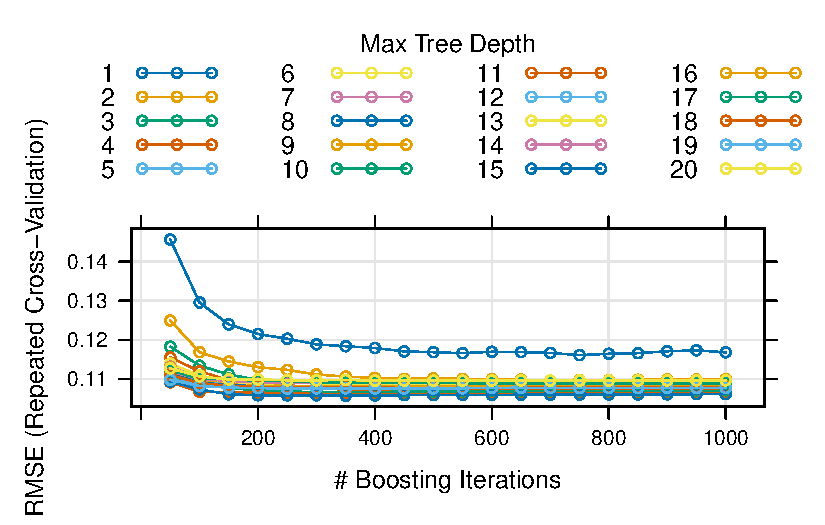
\includegraphics{MachineLearning_StaticPatterNN_Report_files/figure-pdf/hyperparameter-tuning-5.pdf}

\begin{Shaded}
\begin{Highlighting}[]
\NormalTok{gbmModel\_t}\SpecialCharTok{$}\NormalTok{finalModel}
\end{Highlighting}
\end{Shaded}

\begin{verbatim}
A gradient boosted model with gaussian loss function.
350 iterations were performed.
There were 68 predictors of which 57 had non-zero influence.
\end{verbatim}

\begin{Shaded}
\begin{Highlighting}[]
\FunctionTok{slice\_min}\NormalTok{(gbmModel\_t}\SpecialCharTok{$}\NormalTok{results, RMSE)}
\end{Highlighting}
\end{Shaded}

\begin{verbatim}
  shrinkage interaction.depth n.minobsinnode n.trees     RMSE  Rsquared
1       0.1                15             10     350 0.105708 0.8604902
         MAE     RMSESD RsquaredSD      MAESD
1 0.07103516 0.01017044 0.02814312 0.00377382
\end{verbatim}

\begin{Shaded}
\begin{Highlighting}[]
\FunctionTok{slice\_max}\NormalTok{(gbmModel\_t}\SpecialCharTok{$}\NormalTok{results, Rsquared)}
\end{Highlighting}
\end{Shaded}

\begin{verbatim}
  shrinkage interaction.depth n.minobsinnode n.trees     RMSE  Rsquared
1       0.1                15             10     350 0.105708 0.8604902
         MAE     RMSESD RsquaredSD      MAESD
1 0.07103516 0.01017044 0.02814312 0.00377382
\end{verbatim}

\begin{Shaded}
\begin{Highlighting}[]
\CommentTok{\# save.image("./data/hyper\_para\_tuning.RData")}
\end{Highlighting}
\end{Shaded}

\paragraph{Final models}\label{final-models}

\subparagraph{Insights:}\label{insights}

\begin{enumerate}
\def\labelenumi{\arabic{enumi}.}
\item
  Random Forest with Ranger Keeping in mind that splitrule =
  ``extratrees'' ignores the mtry argument (and rather performs random
  selection of variables). This should prevent overfitting and achieves
  a similar performance to mtry = intermediate number and splitrule =
  ``variance''.
\item
  Extreme Gradient Boosted Trees
\item
  Boosted Regression Trees
\end{enumerate}

\begin{Shaded}
\begin{Highlighting}[]
\NormalTok{trainControl }\OtherTok{\textless{}{-}} \FunctionTok{trainControl}\NormalTok{(}
    \AttributeTok{method =} \StringTok{"repeatedcv"}\NormalTok{,}
    \AttributeTok{number =} \DecValTok{10}\NormalTok{,}
    \AttributeTok{repeats =} \DecValTok{3}\NormalTok{,}
    \AttributeTok{savePredictions =} \StringTok{"final"}\NormalTok{,}
    \AttributeTok{returnResamp =} \StringTok{"final"}\NormalTok{,}
    \AttributeTok{verboseIter =} \ConstantTok{FALSE}\NormalTok{,}
    \AttributeTok{index =}\NormalTok{ indices)}

\CommentTok{\# Train ranger model}
\NormalTok{ranger\_grid }\OtherTok{\textless{}{-}} \FunctionTok{expand.grid}\NormalTok{(}
    \AttributeTok{splitrule =} \StringTok{"variance"}\NormalTok{,}
    \AttributeTok{mtry =} \DecValTok{29}\NormalTok{,}
    \AttributeTok{min.node.size =} \DecValTok{5}\NormalTok{)}

\CommentTok{\# tictoc::tic("ranger")}
\CommentTok{\# set.seed(42)}
\CommentTok{\# rangerModel \textless{}{-} train(}
\CommentTok{\#     Jaccard \textasciitilde{} .,}
\CommentTok{\#     data = dat\_train,}
\CommentTok{\#     method = "ranger",}
\CommentTok{\#     trControl = trainControl,}
\CommentTok{\#     importance = "permutation",}
\CommentTok{\#     scale.permutation.importance = TRUE,}
\CommentTok{\#     num.trees = 5000,}
\CommentTok{\#     respect.unordered.factors = TRUE,}
\CommentTok{\#     oob.error = TRUE,}
\CommentTok{\#     tuneGrid = ranger\_grid)}
\CommentTok{\# tictoc::toc()}
\CommentTok{\# saveRDS(rangerModel, "./data/rangerModel\_final.rds")}

\NormalTok{rangerModel }\OtherTok{\textless{}{-}} \FunctionTok{readRDS}\NormalTok{(}\StringTok{"./data/rangerModel\_final.rds"}\NormalTok{)}

\CommentTok{\# Performance checks ======}
\DocumentationTok{\#\# with external data (from initial split)}
\NormalTok{test\_performance\_rf }\OtherTok{\textless{}{-}} \FunctionTok{data.frame}\NormalTok{(}
    \AttributeTok{prediction =} \FunctionTok{predict}\NormalTok{(rangerModel, }\AttributeTok{newdata =}\NormalTok{ dat\_test),}
    \AttributeTok{observed =}\NormalTok{ dat\_test}\SpecialCharTok{$}\NormalTok{Jaccard) }\SpecialCharTok{\%\textgreater{}\%}
    \FunctionTok{mutate}\NormalTok{(}\AttributeTok{test\_error =}\NormalTok{ observed}\SpecialCharTok{{-}}\NormalTok{prediction)}

\FunctionTok{round}\NormalTok{(}\FunctionTok{mean}\NormalTok{(test\_performance\_rf}\SpecialCharTok{$}\NormalTok{test\_error), }\DecValTok{4}\NormalTok{) }
\end{Highlighting}
\end{Shaded}

\begin{verbatim}
[1] 0.0092
\end{verbatim}

\begin{Shaded}
\begin{Highlighting}[]
\CommentTok{\# mean test error = 0.0092 (mtry = 29) // 0.0099 (mtry = 57)}
\FunctionTok{postResample}\NormalTok{(test\_performance\_rf}\SpecialCharTok{$}\NormalTok{observed, }
\NormalTok{test\_performance\_rf}\SpecialCharTok{$}\NormalTok{prediction)}
\end{Highlighting}
\end{Shaded}

\begin{verbatim}
      RMSE   Rsquared        MAE 
0.11673348 0.81964468 0.07412072 
\end{verbatim}

\begin{Shaded}
\begin{Highlighting}[]
\NormalTok{p\_pred\_rangerModel }\OtherTok{\textless{}{-}} \FunctionTok{ggplot}\NormalTok{(}\FunctionTok{aes}\NormalTok{(observed, prediction), }
                             \AttributeTok{data =}\NormalTok{ test\_performance\_rf)}\SpecialCharTok{+}
  \FunctionTok{geom\_point}\NormalTok{()}\SpecialCharTok{+}
  \FunctionTok{geom\_smooth}\NormalTok{(}\AttributeTok{method =} \StringTok{"lm"}\NormalTok{)}\SpecialCharTok{+}
  \FunctionTok{ylim}\NormalTok{(}\DecValTok{0}\NormalTok{,}\DecValTok{1}\NormalTok{)}\SpecialCharTok{+}
  \FunctionTok{xlim}\NormalTok{(}\DecValTok{0}\NormalTok{,}\DecValTok{1}\NormalTok{)}\SpecialCharTok{+}
  \FunctionTok{theme\_bw}\NormalTok{()}

\NormalTok{p\_pred\_rangerModel}
\end{Highlighting}
\end{Shaded}

\begin{verbatim}
`geom_smooth()` using formula = 'y ~ x'
\end{verbatim}

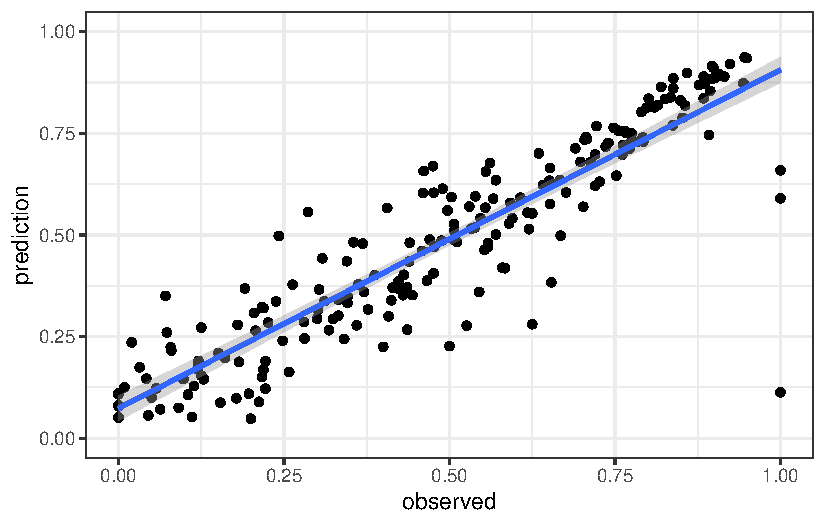
\includegraphics{MachineLearning_StaticPatterNN_Report_files/figure-pdf/final-models-ranger-1.pdf}

\begin{Shaded}
\begin{Highlighting}[]
\DocumentationTok{\#\# custom tuning for xgb:}
\NormalTok{xgb\_grid }\OtherTok{\textless{}{-}} \FunctionTok{expand.grid}\NormalTok{(}
  \AttributeTok{nrounds =} \DecValTok{150}\NormalTok{,}
  \AttributeTok{eta =} \FloatTok{0.3}\NormalTok{,}
  \AttributeTok{max\_depth =} \DecValTok{2}\NormalTok{,}
  \AttributeTok{gamma =} \DecValTok{0}\NormalTok{,}
  \AttributeTok{colsample\_bytree =} \FloatTok{0.6}\NormalTok{,}
  \AttributeTok{min\_child\_weight =} \DecValTok{1}\NormalTok{,}
  \AttributeTok{subsample =} \DecValTok{1}\NormalTok{)}

\CommentTok{\# tictoc::tic("xgb")}
\CommentTok{\# set.seed(42)}
\CommentTok{\# xgbModel \textless{}{-} train(}
\CommentTok{\#     Jaccard \textasciitilde{} .,}
\CommentTok{\#     data = dat\_train,}
\CommentTok{\#     method = "xgbTree",}
\CommentTok{\#     trControl = trainControl,}
\CommentTok{\#     tuneGrid = xgb\_grid)}
\CommentTok{\# tictoc::toc()}
\CommentTok{\# saveRDS(xgbModel, "./data/xgbModel\_final.rds")}

\NormalTok{xgbModel }\OtherTok{\textless{}{-}} \FunctionTok{readRDS}\NormalTok{(}\StringTok{"./data/xgbModel\_final.rds"}\NormalTok{)}

\DocumentationTok{\#\# Check test performance with external data (from initial split)}
\NormalTok{test\_performance\_xgb }\OtherTok{\textless{}{-}} \FunctionTok{data.frame}\NormalTok{(}
    \AttributeTok{prediction =} \FunctionTok{predict}\NormalTok{(xgbModel, }\AttributeTok{newdata =}\NormalTok{ dat\_test),}
    \AttributeTok{observed =}\NormalTok{ dat\_test}\SpecialCharTok{$}\NormalTok{Jaccard) }\SpecialCharTok{\%\textgreater{}\%}
    \FunctionTok{mutate}\NormalTok{(}\AttributeTok{test\_error =}\NormalTok{ observed}\SpecialCharTok{{-}}\NormalTok{prediction)}

\FunctionTok{round}\NormalTok{(}\FunctionTok{mean}\NormalTok{(test\_performance\_xgb}\SpecialCharTok{$}\NormalTok{test\_error), }\DecValTok{4}\NormalTok{) }
\end{Highlighting}
\end{Shaded}

\begin{verbatim}
[1] 0.01
\end{verbatim}

\begin{Shaded}
\begin{Highlighting}[]
\CommentTok{\# mean test error = }
\FunctionTok{postResample}\NormalTok{(test\_performance\_xgb}\SpecialCharTok{$}\NormalTok{observed, }
\NormalTok{test\_performance\_xgb}\SpecialCharTok{$}\NormalTok{prediction)}
\end{Highlighting}
\end{Shaded}

\begin{verbatim}
      RMSE   Rsquared        MAE 
0.12120562 0.80930929 0.07596198 
\end{verbatim}

\begin{Shaded}
\begin{Highlighting}[]
\NormalTok{p\_pred\_xgbModel }\OtherTok{\textless{}{-}} \FunctionTok{ggplot}\NormalTok{(}\FunctionTok{aes}\NormalTok{(observed, prediction), }\AttributeTok{data =}\NormalTok{ test\_performance\_xgb)}\SpecialCharTok{+}
    \FunctionTok{geom\_point}\NormalTok{()}\SpecialCharTok{+}
    \FunctionTok{geom\_smooth}\NormalTok{(}\AttributeTok{method =} \StringTok{"lm"}\NormalTok{)}\SpecialCharTok{+}
    \FunctionTok{ylim}\NormalTok{(}\DecValTok{0}\NormalTok{,}\DecValTok{1}\NormalTok{)}\SpecialCharTok{+}
    \FunctionTok{xlim}\NormalTok{(}\DecValTok{0}\NormalTok{,}\DecValTok{1}\NormalTok{)}\SpecialCharTok{+}
    \FunctionTok{theme\_bw}\NormalTok{()}
\NormalTok{p\_pred\_xgbModel}
\end{Highlighting}
\end{Shaded}

\begin{verbatim}
`geom_smooth()` using formula = 'y ~ x'
\end{verbatim}

\begin{verbatim}
Warning: Removed 2 rows containing non-finite outside the scale range
(`stat_smooth()`).
\end{verbatim}

\begin{verbatim}
Warning: Removed 2 rows containing missing values or values outside the scale range
(`geom_point()`).
\end{verbatim}

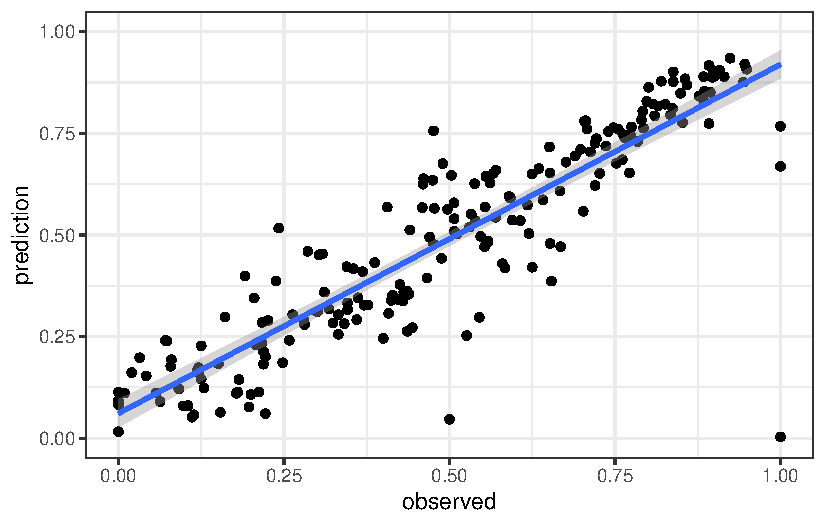
\includegraphics{MachineLearning_StaticPatterNN_Report_files/figure-pdf/final-models-xgb-1.pdf}

\begin{Shaded}
\begin{Highlighting}[]
\CommentTok{\# Train gbm model}
\NormalTok{gbm\_grid }\OtherTok{\textless{}{-}}  \FunctionTok{expand.grid}\NormalTok{(}\AttributeTok{interaction.depth =} \DecValTok{15}\NormalTok{, }
                        \AttributeTok{n.trees =} \DecValTok{350}\NormalTok{, }
                        \AttributeTok{shrinkage =} \FloatTok{0.1}\NormalTok{,}
                        \AttributeTok{n.minobsinnode =} \DecValTok{10}\NormalTok{)}
\CommentTok{\# tictoc::tic("gbm")}
\CommentTok{\# set.seed(42)}
\CommentTok{\# gbmModel \textless{}{-} train(}
\CommentTok{\#     Jaccard \textasciitilde{} .,}
\CommentTok{\#     data = dat\_train,}
\CommentTok{\#     method = "gbm",}
\CommentTok{\#     trControl = trainControl,}
\CommentTok{\#     tuneGrid = gbm\_grid,}
\CommentTok{\#     verbose = FALSE)}
\CommentTok{\# tictoc::toc()}
\CommentTok{\# saveRDS(gbmModel, "./data/gbmModel\_final.rds")}

\NormalTok{gbmModel }\OtherTok{\textless{}{-}} \FunctionTok{readRDS}\NormalTok{(}\StringTok{"./data/gbmModel\_final.rds"}\NormalTok{)}

\DocumentationTok{\#\# Check test performance with external data (from initial split)}
\NormalTok{test\_performance\_gbm }\OtherTok{\textless{}{-}} \FunctionTok{data.frame}\NormalTok{(}
    \AttributeTok{prediction =} \FunctionTok{predict}\NormalTok{(gbmModel, }\AttributeTok{newdata =}\NormalTok{ dat\_test),}
    \AttributeTok{observed =}\NormalTok{ dat\_test}\SpecialCharTok{$}\NormalTok{Jaccard) }\SpecialCharTok{\%\textgreater{}\%}
    \FunctionTok{mutate}\NormalTok{(}\AttributeTok{test\_error =}\NormalTok{ observed}\SpecialCharTok{{-}}\NormalTok{prediction)}

\FunctionTok{round}\NormalTok{(}\FunctionTok{mean}\NormalTok{(test\_performance\_gbm}\SpecialCharTok{$}\NormalTok{test\_error), }\DecValTok{4}\NormalTok{) }
\end{Highlighting}
\end{Shaded}

\begin{verbatim}
[1] 0.0094
\end{verbatim}

\begin{Shaded}
\begin{Highlighting}[]
\CommentTok{\# mean test error = }
\FunctionTok{postResample}\NormalTok{(test\_performance\_gbm}\SpecialCharTok{$}\NormalTok{observed, test\_performance\_gbm}\SpecialCharTok{$}\NormalTok{prediction)}
\end{Highlighting}
\end{Shaded}

\begin{verbatim}
     RMSE  Rsquared       MAE 
0.1192561 0.8168099 0.0740695 
\end{verbatim}

\begin{Shaded}
\begin{Highlighting}[]
\NormalTok{p\_pred\_gbmModel }\OtherTok{\textless{}{-}} \FunctionTok{ggplot}\NormalTok{(}\FunctionTok{aes}\NormalTok{(observed, prediction), }\AttributeTok{data =}\NormalTok{ test\_performance\_gbm)}\SpecialCharTok{+}
    \FunctionTok{geom\_point}\NormalTok{()}\SpecialCharTok{+}
    \FunctionTok{geom\_smooth}\NormalTok{(}\AttributeTok{method =} \StringTok{"lm"}\NormalTok{)}\SpecialCharTok{+}
    \FunctionTok{ylim}\NormalTok{(}\DecValTok{0}\NormalTok{,}\DecValTok{1}\NormalTok{)}\SpecialCharTok{+}
    \FunctionTok{xlim}\NormalTok{(}\DecValTok{0}\NormalTok{,}\DecValTok{1}\NormalTok{)}\SpecialCharTok{+}
    \FunctionTok{theme\_bw}\NormalTok{()}
\NormalTok{p\_pred\_gbmModel}
\end{Highlighting}
\end{Shaded}

\begin{verbatim}
`geom_smooth()` using formula = 'y ~ x'
\end{verbatim}

\begin{verbatim}
Warning: Removed 4 rows containing non-finite outside the scale range
(`stat_smooth()`).
\end{verbatim}

\begin{verbatim}
Warning: Removed 4 rows containing missing values or values outside the scale range
(`geom_point()`).
\end{verbatim}

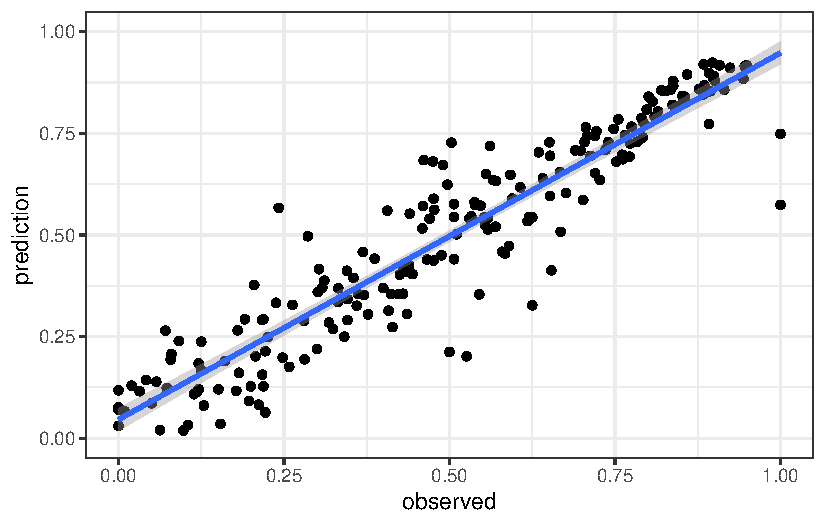
\includegraphics{MachineLearning_StaticPatterNN_Report_files/figure-pdf/final-models-gbm-1.pdf}

\subsubsection{Compare models}\label{compare-models}

\begin{Shaded}
\begin{Highlighting}[]
\CommentTok{\# Prediction error for test data ============}
\NormalTok{test\_error\_all }\OtherTok{\textless{}{-}} \FunctionTok{data.frame}\NormalTok{(}
    \AttributeTok{observed =}\NormalTok{ dat\_test}\SpecialCharTok{$}\NormalTok{Jaccard,}
    \AttributeTok{pred\_ranger =} \FunctionTok{predict}\NormalTok{(rangerModel, }\AttributeTok{newdata=}\NormalTok{dat\_test),}
    \AttributeTok{pred\_xgb =} \FunctionTok{predict}\NormalTok{(xgbModel, }\AttributeTok{newdata=}\NormalTok{dat\_test),}
    \AttributeTok{pred\_gbm =} \FunctionTok{predict}\NormalTok{(gbmModel, }\AttributeTok{newdata=}\NormalTok{dat\_test)) }\SpecialCharTok{\%\textgreater{}\%}
    \FunctionTok{mutate}\NormalTok{(}
        \AttributeTok{test\_error\_ranger =}\NormalTok{ observed}\SpecialCharTok{{-}}\NormalTok{pred\_ranger,}
        \AttributeTok{test\_error\_xgb =}\NormalTok{ observed}\SpecialCharTok{{-}}\NormalTok{pred\_xgb,}
        \AttributeTok{test\_error\_gbm =}\NormalTok{ observed}\SpecialCharTok{{-}}\NormalTok{pred\_gbm)}

\FunctionTok{round}\NormalTok{(}\FunctionTok{mean}\NormalTok{(test\_error\_all}\SpecialCharTok{$}\NormalTok{test\_error\_ranger),}\DecValTok{4}\NormalTok{)}
\end{Highlighting}
\end{Shaded}

\begin{verbatim}
[1] 0.0092
\end{verbatim}

\begin{Shaded}
\begin{Highlighting}[]
\FunctionTok{round}\NormalTok{(}\FunctionTok{mean}\NormalTok{(test\_error\_all}\SpecialCharTok{$}\NormalTok{test\_error\_xgb),}\DecValTok{4}\NormalTok{)}
\end{Highlighting}
\end{Shaded}

\begin{verbatim}
[1] 0.01
\end{verbatim}

\begin{Shaded}
\begin{Highlighting}[]
\FunctionTok{round}\NormalTok{(}\FunctionTok{mean}\NormalTok{(test\_error\_all}\SpecialCharTok{$}\NormalTok{test\_error\_gbm),}\DecValTok{4}\NormalTok{)}
\end{Highlighting}
\end{Shaded}

\begin{verbatim}
[1] 0.0094
\end{verbatim}

\begin{Shaded}
\begin{Highlighting}[]
\FunctionTok{print}\NormalTok{(test\_error\_all)}
\end{Highlighting}
\end{Shaded}

\begin{verbatim}
    observed pred_ranger     pred_xgb     pred_gbm test_error_ranger
1      0.877  0.86910115  0.841720462  0.858786806       0.007898850
2      0.558  0.48012318  0.482135415  0.541184787       0.077876817
3      0.885  0.87104168  0.853786528  0.868535385       0.013958323
4      0.301  0.31540890  0.311780423  0.359522282      -0.014408897
5      0.570  0.50103061  0.543499231  0.520473158       0.068969387
6      0.625  0.28030096  0.420663059  0.327032693       0.344699040
7      0.436  0.37108671  0.361571074  0.409046332       0.064913290
8      0.722  0.76784859  0.736952543  0.755024925      -0.045848587
9      0.258  0.16296630  0.240690067  0.175508246       0.095033700
10     0.507  0.48713397  0.540104508  0.544041914       0.019866030
11     0.341  0.24414757  0.281917453  0.249880444       0.096852433
12     0.727  0.63123632  0.651297629  0.635399655       0.095763683
13     0.849  0.83080491  0.848294377  0.818866830       0.018195090
14     0.748  0.76349889  0.764104962  0.760798612      -0.015498887
15     0.300  0.29415898  0.311248749  0.219716116       0.005841017
16     0.346  0.33306361  0.332728505  0.342273499       0.012936393
17     0.091  0.07472768  0.121196210  0.239060621       0.016272320
18     0.346  0.34891770  0.316328496  0.290406102      -0.002917697
19     0.470  0.48882009  0.494753987  0.539752581      -0.018820093
20     0.676  0.60464716  0.678787291  0.603514461       0.071352843
21     0.387  0.40107793  0.432122797  0.441737877      -0.014077927
22     0.217  0.15044600  0.233548597  0.156367590       0.066554000
23     0.125  0.15411696  0.145354167  0.237417415      -0.029116960
24     0.332  0.30153652  0.255690753  0.335072105       0.030463477
25     0.000  0.08064779  0.091773041  0.075731780      -0.080647787
26     0.045  0.05599648 -0.022524470 -0.082739111      -0.010996477
27     0.212  0.08951877  0.113322906  0.082412768       0.122481233
28     0.362  0.37842884  0.345532566  0.355040688      -0.016428840
29     0.488  0.48584563  0.442314416  0.450168069       0.002154367
30     0.915  0.88973184  0.889276743  0.857246508       0.025268157
31     0.620  0.51408998  0.503365517  0.543782820       0.105910023
32     0.801  0.83546678  0.863279164  0.840257613      -0.034466783
33     0.459  0.46073617  0.567396343  0.515950423      -0.001736167
34     0.439  0.43456290  0.354126155  0.424658562       0.004437100
35     0.834  0.83869868  0.795241237  0.857388005      -0.004698680
36     0.698  0.67986528  0.710411429  0.707072846       0.018134717
37     0.408  0.30011007  0.306941986  0.313462377       0.107889927
38     0.226  0.28453677  0.289481640  0.249399858      -0.058536773
39     0.820  0.86415662  0.878294766  0.856016442      -0.044156620
40     0.798  0.81325615  0.828865051  0.808533569      -0.015256147
41     0.838  0.86107262  0.901359499  0.867291719      -0.023072617
42     0.706  0.74088902  0.781144619  0.764759982      -0.034889023
43     0.884  0.88987952  0.889441192  0.919608197      -0.005879523
44     0.425  0.36598447  0.378189653  0.402398264       0.059015527
45     0.651  0.63359957  0.716534138  0.727723211       0.017400430
46     0.219  0.32013352  0.213798508  0.292581305      -0.101133517
47     0.740  0.72643536  0.754374385  0.728496162       0.013564640
48     0.071  0.35003889  0.240456909  0.264654790      -0.279038887
49     0.538  0.51788237  0.626019239  0.580837016       0.020117627
50     0.898  0.88492383  0.905012965  0.885763105       0.013076173
51     0.180  0.27870014  0.113524258  0.265522896      -0.098700143
52     0.191  0.36816647  0.398833275  0.292474353      -0.177166473
53     0.766  0.75162881  0.738634706  0.745274287       0.014371190
54     0.460  0.60283619  0.624736845  0.571364915      -0.142836193
55     0.490  0.61388772  0.675599635  0.671810025      -0.123887717
56     0.242  0.49746486  0.517009079  0.566553308      -0.255464863
57     1.000  0.59001967  0.668556631  0.573931872       0.409980330
58     0.793  0.72978320  0.762712002  0.776647085       0.063216800
59     0.503  0.59330830  0.646690905  0.727373407      -0.090308303
60     0.461  0.65727545  0.638278484  0.684229825      -0.196275447
61     0.607  0.59173842  0.535432339  0.617309134       0.015261580
62     0.652  0.57664901  0.478944153  0.595494186       0.075350987
63     0.511  0.48267249  0.502158523  0.501536117       0.028327510
64     0.539  0.59488800  0.535161376  0.573274988      -0.055887997
65     0.784  0.72880292  0.729910254  0.729392487       0.055197077
66     0.755  0.75688083  0.760203242  0.784473742      -0.001880830
67     0.924  0.92086041  0.934829056  0.911307401       0.003139587
68     0.720  0.69799839  0.621882617  0.743523346       0.022001610
69     0.020  0.23569131  0.161473483  0.129153041      -0.215691310
70     0.570  0.63471052  0.659243643  0.633114001      -0.064710523
71     0.545  0.35993530  0.297215998  0.353748063       0.185064703
72     0.406  0.56609778  0.568368733  0.559708371      -0.160097777
73     0.761  0.69776270  0.685188293  0.697241017       0.063237300
74     0.369  0.47878383  0.409776270  0.458048628      -0.109783830
75     0.308  0.44259404  0.453329891  0.370469736      -0.134594037
76     0.837  0.76938678  0.811477840  0.820033739       0.067613217
77     0.555  0.65578816  0.644153655  0.650202211      -0.100788163
78     0.423  0.38596047  0.340562016  0.354553602       0.037039533
79     0.949  0.93492990  0.907812417  0.917061603       0.014070103
80     0.773  0.72618088  0.747302651  0.725088176       0.046819117
81     0.414  0.37066815  0.351498842  0.273304010       0.043331853
82     0.946  0.93691120  0.920259655  0.915239073       0.009088803
83     0.466  0.38759309  0.393931627  0.439366795       0.078406910
84     0.807  0.81726822  0.822605491  0.828350607      -0.010268220
85     0.894  0.85429762  0.850715041  0.853734671       0.039702380
86     0.444  0.35197273  0.272128493  0.403816151       0.092027270
87     0.635  0.70065961  0.663365901  0.703276547      -0.065659607
88     0.765  0.75605629  0.738009155  0.746265610       0.008943710
89     0.412  0.33923076  0.338842958  0.354797895       0.072769240
90     0.533  0.51565367  0.551553607  0.546238108       0.017346333
91     0.752  0.64571932  0.676178813  0.680260891       0.106280683
92     0.497  0.56011681  0.563128710  0.623779664      -0.063116807
93     0.263  0.37790796  0.304043263  0.327928624      -0.114907957
94     0.641  0.62307031  0.586523890  0.639223549       0.017929687
95     0.345  0.43526692  0.421977609  0.412014844      -0.090266923
96     0.073  0.26012574  0.239444256  0.122945624      -0.187125740
97     0.815  0.82016266  0.817191660  0.803985255      -0.005162657
98     0.720  0.62131033  0.725555241  0.651657369       0.098689667
99     0.248  0.23956347  0.185565591  0.198309531       0.008436527
100    0.618  0.55472222  0.573590159  0.533958493       0.063277780
101    0.440  0.48082232  0.512277305  0.552094417      -0.040822323
102    0.884  0.83631774  0.830074847  0.846190012       0.047682263
103    0.708  0.73623070  0.760659456  0.743659358      -0.028230697
104    0.476  0.40584418  0.477438539  0.437174028       0.070155823
105    0.790  0.80254295  0.783323467  0.787300016      -0.012542953
106    0.826  0.83477398  0.821740568  0.853822802      -0.008773980
107    0.584  0.41825557  0.419202387  0.454187154       0.165744433
108    0.476  0.60380890  0.756092131  0.589052012      -0.127808897
109    0.592  0.57897874  0.590857685  0.647751717       0.013021260
110    0.355  0.48212656  0.416800290  0.394352501      -0.127126560
111    0.892  0.74550810  0.773891807  0.772629240       0.146491903
112    0.901  0.88646249  0.891810775  0.879675203       0.014537513
113    0.908  0.89500705  0.905218959  0.917363561       0.012992953
114    0.595  0.54135423  0.536568224  0.589614652       0.053645773
115    0.792  0.73989600  0.804139674  0.740003434       0.052104000
116    0.762  0.72122780  0.747630060  0.686191201       0.040772203
117    0.690  0.71313634  0.694381237  0.707939672      -0.023136337
118    0.892  0.88389528  0.916926503  0.898616456       0.008104720
119    0.736  0.71749193  0.718703866  0.710037212       0.018508067
120    0.852  0.78799691  0.776563168  0.841912974       0.064003087
121    0.702  0.56941263  0.558282137  0.585912305       0.132587373
122    0.009  0.12496442  0.110772729  0.066668190      -0.115964417
123    0.580  0.41945107  0.429435819  0.458557754       0.160548930
124    0.475  0.66906487  0.634434640  0.680962185      -0.194064870
125    0.668  0.49828451  0.471017420  0.507703484       0.169715493
126    0.154  0.08735871  0.063460365  0.035255484       0.066641290
127    1.000  0.11278980  0.003010696 -0.018252809       0.887210200
128    0.129  0.14480389  0.123093404  0.080201211      -0.015803893
129    0.507  0.52721160  0.579143703  0.575620127      -0.020211597
130    0.500  0.22648847  0.046460938  0.212075718       0.273511527
131    0.625  0.55296068  0.649796605  0.543188243       0.072039320
132    0.197  0.10949944  0.076905474  0.091770907       0.087500560
133    0.430  0.35183315  0.337726593  0.355360207       0.078166847
134    0.222  0.12185026  0.060609128  0.063247002       0.100149743
135    0.654  0.38322946  0.386361718  0.412812582       0.270770537
136    0.217  0.32311244  0.284754127  0.290422234      -0.106112443
137    0.810  0.81400921  0.792983353  0.791396920      -0.004009207
138    0.530  0.56997982  0.519229829  0.540517827      -0.039979823
139    0.713  0.67901589  0.704296529  0.694385580       0.033984107
140    0.436  0.26715790  0.262925655  0.305519341       0.168842103
141    0.114  0.12848735  0.057560798  0.108079024      -0.014487350
142    0.477  0.47146091  0.565632224  0.561845160       0.005539087
143    0.222  0.18949855  0.200443968  0.214014539       0.032501447
144    0.079  0.22338234  0.176939458  0.193408353      -0.144382340
145    1.000  0.65905833  0.767441094  0.748657346       0.340941667
146    0.000  0.07861809  0.016103623  0.070593616      -0.078618090
147    0.032  0.17447724  0.197845399  0.115631305      -0.142477240
148    0.772  0.71265212  0.652894974  0.692631159       0.059347880
149    0.667  0.63529303  0.607956767  0.655229002       0.031706967
150    0.944  0.87344407  0.875961602  0.884405437       0.070555927
151    0.561  0.67721536  0.627638161  0.719035624      -0.116215360
152    0.652  0.66454380  0.652679980  0.694946923      -0.012543803
153    0.286  0.55674848  0.459790528  0.496832595      -0.270748477
154    0.553  0.46325102  0.470841795  0.544102391       0.089748980
155    0.125  0.27211704  0.227275342  0.167126126      -0.147117037
156    0.507  0.51107489  0.508873641  0.440208183      -0.004074887
157    0.566  0.58930015  0.651429594  0.634927441      -0.023300147
158    0.590  0.52809865  0.594880223  0.473219075       0.061901350
159    0.098  0.14547843  0.079473920  0.018847185      -0.047478433
160    0.400  0.22468527  0.245468497  0.369204824       0.175314733
161    0.280  0.28541792  0.292349100  0.288906040      -0.005417917
162    0.080  0.21578336  0.193099767  0.207109726      -0.135783363
163    0.360  0.27767515  0.291874230  0.325875361       0.082324853
164    0.526  0.27679073  0.252609611  0.201502665       0.249209267
165    0.311  0.33723835  0.359469295  0.387422999      -0.026238347
166    0.105  0.10714211  0.080056250  0.032888783      -0.002142110
167    0.119  0.16957647  0.165320158  0.114147817      -0.050576473
168    0.151  0.20948050  0.183253795  0.120013871      -0.058480500
169    0.303  0.36571264  0.451199919  0.415739965      -0.062712640
170    0.050  0.09983216 -0.002156811  0.085693337      -0.049832160
171    0.377  0.31677662  0.327817053  0.304593495       0.060223377
172    0.121  0.19011618  0.161437586  0.184124998      -0.069116177
173    0.205  0.30832203  0.344760239  0.377283415      -0.103322030
174    0.000  0.05087741  0.092464112 -0.059957205      -0.050877410
175    0.161  0.19699397  0.298553467  0.189903396      -0.035993973
176    0.899  0.91089704  0.897774637  0.891297186      -0.011897043
177    0.238  0.33656437  0.387012482  0.333138039      -0.098564373
178    0.554  0.56719794  0.568757296  0.524736508      -0.013197940
179    0.775  0.74984881  0.765696526  0.766274963       0.025151190
180    0.558  0.46962757  0.484941751  0.513523491       0.088372427
181    0.219  0.16849843  0.182067677  0.127357297       0.050501570
182    0.547  0.54150806  0.496261269  0.571951389       0.005491937
183    0.182  0.18807953  0.144231349  0.160997459      -0.006079527
184    0.121  0.18231300  0.173660427  0.120611716      -0.061312997
185    0.207  0.26460809  0.230161041  0.201393236      -0.057608093
186    0.281  0.24535114  0.279576063  0.193824598       0.035648863
187    0.897  0.91565807  0.887728870  0.923723818      -0.018658070
188    0.000  0.10786734  0.113310881  0.030342309      -0.107867337
189    0.838  0.88513168  0.876823425  0.878841665      -0.047131677
190    0.042  0.14647043  0.153313279  0.142909866      -0.104470430
191    0.178  0.09807436  0.110509343  0.116261748       0.079925643
192    0.000  0.11014081  0.082849048  0.117764815      -0.110140807
193    0.371  0.36028605  0.326993763  0.352393598       0.010713947
194    0.856  0.81850005  0.884268463  0.839804391       0.037499950
195    0.200  0.04796456  0.107347690  0.127491971       0.152035443
196    0.332  0.34058516  0.303889722  0.368946857      -0.008585160
197    0.318  0.26568185  0.317851275  0.284302967       0.052318153
198    0.111  0.05226267  0.051669590 -0.009616781       0.058737330
199    0.324  0.29331427  0.283216536  0.268791567       0.030685730
200    0.057  0.12269151  0.111600265  0.139142343      -0.065691507
201    0.704  0.73435895  0.780214429  0.728729487      -0.030358953
202    0.431  0.40204196  0.358864278  0.419013115       0.028958040
203    0.859  0.89873129  0.868581951  0.894715505      -0.039731293
204    0.063  0.07099401  0.089766234  0.019694592      -0.007994007
    test_error_xgb test_error_gbm
1     0.0352795382    0.018213194
2     0.0758645849    0.016815213
3     0.0312134719    0.016464615
4    -0.0107804229   -0.058522282
5     0.0265007687    0.049526842
6     0.2043369412    0.297967307
7     0.0744289265    0.026953668
8    -0.0149525433   -0.033024925
9     0.0173099326    0.082491754
10   -0.0331045084   -0.037041914
11    0.0590825472    0.091119556
12    0.0757023711    0.091600345
13    0.0007056227    0.030133170
14   -0.0161049623   -0.012798612
15   -0.0112487495    0.080283884
16    0.0132714949    0.003726501
17   -0.0301962104   -0.148060621
18    0.0296715043    0.055593898
19   -0.0247539866   -0.069752581
20   -0.0027872910    0.072485539
21   -0.0451227968   -0.054737877
22   -0.0165485965    0.060632410
23   -0.0203541666   -0.112417415
24    0.0763092465   -0.003072105
25   -0.0917730406   -0.075731780
26    0.0675244705    0.127739111
27    0.0986770938    0.129587232
28    0.0164674337    0.006959312
29    0.0456855838    0.037831931
30    0.0257232571    0.057753492
31    0.1166344833    0.076217180
32   -0.0622791638   -0.039257613
33   -0.1083963428   -0.056950423
34    0.0848738446    0.014341438
35    0.0387587633   -0.023388005
36   -0.0124114294   -0.009072846
37    0.1010580139    0.094537623
38   -0.0634816399   -0.023399858
39   -0.0582947659   -0.036016442
40   -0.0308650513   -0.010533569
41   -0.0633594985   -0.029291719
42   -0.0751446190   -0.058759982
43   -0.0054411922   -0.035608197
44    0.0468103468    0.022601736
45   -0.0655341377   -0.076723211
46    0.0052014920   -0.073581305
47   -0.0143743849    0.011503838
48   -0.1694569089   -0.193654790
49   -0.0880192394   -0.042837016
50   -0.0070129652    0.012236895
51    0.0664757419   -0.085522896
52   -0.2078332748   -0.101474353
53    0.0273652945    0.020725713
54   -0.1647368455   -0.111364915
55   -0.1855996346   -0.181810025
56   -0.2750090795   -0.324553308
57    0.3314433694    0.426068128
58    0.0302879982    0.016352915
59   -0.1436909051   -0.224373407
60   -0.1772784843   -0.223229825
61    0.0715676613   -0.010309134
62    0.1730558474    0.056505814
63    0.0088414774    0.009463883
64    0.0038386240   -0.034274988
65    0.0540897455    0.054607513
66   -0.0052032423   -0.029473742
67   -0.0108290563    0.012692599
68    0.0981173825   -0.023523346
69   -0.1414734828   -0.109153041
70   -0.0892436433   -0.063114001
71    0.2477840018    0.191251937
72   -0.1623687329   -0.153708371
73    0.0758117065    0.063758983
74   -0.0407762704   -0.089048628
75   -0.1453298910   -0.062469736
76    0.0255221601    0.016966261
77   -0.0891536546   -0.095202211
78    0.0824379842    0.068446398
79    0.0411875834    0.031938397
80    0.0256973486    0.047911824
81    0.0625011578    0.140695990
82    0.0257403455    0.030760927
83    0.0720683727    0.026633205
84   -0.0156054907   -0.021350607
85    0.0432849588    0.040265329
86    0.1718715074    0.040183849
87   -0.0283659005   -0.068276547
88    0.0269908452    0.018734390
89    0.0731570418    0.057202105
90   -0.0185536070   -0.013238108
91    0.0758211870    0.071739109
92   -0.0661287098   -0.126779664
93   -0.0410432632   -0.064928624
94    0.0544761095    0.001776451
95   -0.0769776094   -0.067014844
96   -0.1664442558   -0.049945624
97   -0.0021916604    0.011014745
98   -0.0055552411    0.068342631
99    0.0624344091    0.049690469
100   0.0444098406    0.084041507
101  -0.0722773051   -0.112094417
102   0.0539251533    0.037809988
103  -0.0526594563   -0.035659358
104  -0.0014385393    0.038825972
105   0.0066765332    0.002699984
106   0.0042594323   -0.027822802
107   0.1647976127    0.129812846
108  -0.2800921311   -0.113052012
109   0.0011423154   -0.055751717
110  -0.0618002903   -0.039352501
111   0.1181081934    0.119370760
112   0.0091892252    0.021324797
113   0.0027810411   -0.009363561
114   0.0584317756    0.005385348
115  -0.0121396737    0.051996566
116   0.0143699403    0.075808799
117  -0.0043812370   -0.017939672
118  -0.0249265032   -0.006616456
119   0.0172961340    0.025962788
120   0.0754368324    0.010087026
121   0.1437178631    0.116087695
122  -0.1017727289   -0.057668190
123   0.1505641806    0.121442246
124  -0.1594346404   -0.205962185
125   0.1969825797    0.160296516
126   0.0905396351    0.118744516
127   0.9969893037    1.018252809
128   0.0059065961    0.048798789
129  -0.0721437030   -0.068620127
130   0.4535390623    0.287924282
131  -0.0247966051    0.081811757
132   0.1200945259    0.105229093
133   0.0922734070    0.074639793
134   0.1613908717    0.158752998
135   0.2676382818    0.241187418
136  -0.0677541273   -0.073422234
137   0.0170166469    0.018603080
138   0.0107701707   -0.010517827
139   0.0087034707    0.018614420
140   0.1730743454    0.130480659
141   0.0564392022    0.005920976
142  -0.0886322241   -0.084845160
143   0.0215560318    0.007985461
144  -0.0979394577   -0.114408353
145   0.2325589061    0.251342654
146  -0.0161036234   -0.070593616
147  -0.1658453994   -0.083631305
148   0.1191050262    0.079368841
149   0.0590432329    0.011770998
150   0.0680383983    0.059594563
151  -0.0666381612   -0.158035624
152  -0.0006799798   -0.042946923
153  -0.1737905278   -0.210832595
154   0.0821582048    0.008897609
155  -0.1022753417   -0.042126126
156  -0.0018736415    0.066791817
157  -0.0854295936   -0.068927441
158  -0.0048802233    0.116780925
159   0.0185260798    0.079152815
160   0.1545315027    0.030795176
161  -0.0123491001   -0.008906040
162  -0.1130997670   -0.127109726
163   0.0681257701    0.034124639
164   0.2733903894    0.324497335
165  -0.0484692945   -0.076422999
166   0.0249437499    0.072111217
167  -0.0463201580    0.004852183
168  -0.0322537949    0.030986129
169  -0.1481999190   -0.112739965
170   0.0521568113   -0.035693337
171   0.0491829474    0.072406505
172  -0.0404375859   -0.063124998
173  -0.1397602391   -0.172283415
174  -0.0924641117    0.059957205
175  -0.1375534668   -0.028903396
176   0.0012253633    0.007702814
177  -0.1490124817   -0.095138039
178  -0.0147572956    0.029263492
179   0.0093034744    0.008725037
180   0.0730582492    0.044476509
181   0.0369323226    0.091642703
182   0.0507387311   -0.024951389
183   0.0377686508    0.021002541
184  -0.0526604273    0.000388284
185  -0.0231610410    0.005606764
186   0.0014239368    0.087175402
187   0.0092711301   -0.026723818
188  -0.1133108810   -0.030342309
189  -0.0388234253   -0.040841665
190  -0.1113132792   -0.100909866
191   0.0674906566    0.061738252
192  -0.0828490481   -0.117764815
193   0.0440062366    0.018606402
194  -0.0282684627    0.016195609
195   0.0926523104    0.072508029
196   0.0281102784   -0.036946857
197   0.0001487248    0.033697033
198   0.0593304098    0.120616781
199   0.0407834640    0.055208433
200  -0.0546002649   -0.082142343
201  -0.0762144289   -0.024729487
202   0.0721357224    0.011986885
203  -0.0095819507   -0.035715505
204  -0.0267662342    0.043305408
\end{verbatim}

\begin{Shaded}
\begin{Highlighting}[]
\CommentTok{\# Variable importance ============}
\NormalTok{imp\_rf }\OtherTok{\textless{}{-}} \FunctionTok{varImp}\NormalTok{(rangerModel, }\AttributeTok{type=}\DecValTok{1}\NormalTok{)}\SpecialCharTok{$}\NormalTok{importance }\SpecialCharTok{\%\textgreater{}\%} 
    \FunctionTok{rename}\NormalTok{(}\StringTok{"Imp\_ranger"} \OtherTok{=} \StringTok{"Overall"}\NormalTok{)}
\NormalTok{imp\_xgb }\OtherTok{\textless{}{-}} \FunctionTok{varImp}\NormalTok{(xgbModel, }\AttributeTok{type=}\DecValTok{1}\NormalTok{)}\SpecialCharTok{$}\NormalTok{importance }\SpecialCharTok{\%\textgreater{}\%} 
    \FunctionTok{rename}\NormalTok{(}\StringTok{"Imp\_xgb"} \OtherTok{=} \StringTok{"Overall"}\NormalTok{)}
\NormalTok{imp\_gbm }\OtherTok{\textless{}{-}} \FunctionTok{varImp}\NormalTok{(gbmModel, }\AttributeTok{type=}\DecValTok{1}\NormalTok{)}\SpecialCharTok{$}\NormalTok{importance }\SpecialCharTok{\%\textgreater{}\%} 
    \FunctionTok{rename}\NormalTok{(}\StringTok{"Imp\_gbm"} \OtherTok{=} \StringTok{"Overall"}\NormalTok{)}

\NormalTok{imp\_temp }\OtherTok{\textless{}{-}} \FunctionTok{merge}\NormalTok{(imp\_rf, imp\_xgb, }\AttributeTok{by =} \StringTok{"row.names"}\NormalTok{, }\AttributeTok{all =} \ConstantTok{TRUE}\NormalTok{)}
\NormalTok{imp\_all }\OtherTok{\textless{}{-}} \FunctionTok{merge}\NormalTok{(imp\_temp, imp\_gbm, }\AttributeTok{by.x =} \StringTok{"Row.names"}\NormalTok{, }\AttributeTok{by.y =} \StringTok{"row.names"}\NormalTok{, }\AttributeTok{all =} \ConstantTok{TRUE}\NormalTok{) }\SpecialCharTok{\%\textgreater{}\%} \FunctionTok{mutate\_if}\NormalTok{(is.numeric, round, }\DecValTok{2}\NormalTok{) }\SpecialCharTok{\%\textgreater{}\%}
\FunctionTok{arrange}\NormalTok{(}\FunctionTok{desc}\NormalTok{(Imp\_ranger))}

\CommentTok{\# Compare models using resamples ============}
\NormalTok{resamples }\OtherTok{\textless{}{-}} \FunctionTok{resamples}\NormalTok{(}\FunctionTok{list}\NormalTok{(}
    \AttributeTok{ranger =}\NormalTok{ rangerModel,}
    \AttributeTok{xgbTree =}\NormalTok{ xgbModel,}
    \AttributeTok{gbm =}\NormalTok{ gbmModel))}

\FunctionTok{summary}\NormalTok{(resamples)}
\end{Highlighting}
\end{Shaded}

\begin{verbatim}

Call:
summary.resamples(object = resamples)

Models: ranger, xgbTree, gbm 
Number of resamples: 10 

MAE 
              Min.    1st Qu.     Median       Mean    3rd Qu.       Max. NA's
ranger  0.07085573 0.07149706 0.07401418 0.07487850 0.07757316 0.08320233    0
xgbTree 0.06712120 0.07317461 0.07642445 0.07640729 0.07982718 0.08665615    0
gbm     0.05985385 0.07001672 0.07138808 0.07277912 0.07571622 0.08446322    0

RMSE 
              Min.   1st Qu.    Median     Mean   3rd Qu.      Max. NA's
ranger  0.09924501 0.1045033 0.1096959 0.112203 0.1183738 0.1307425    0
xgbTree 0.09655579 0.1081520 0.1123912 0.114011 0.1188310 0.1367883    0
gbm     0.09928899 0.1017205 0.1053075 0.109023 0.1100013 0.1362439    0

Rsquared 
             Min.   1st Qu.    Median      Mean   3rd Qu.      Max. NA's
ranger  0.7857122 0.8263894 0.8536590 0.8434265 0.8625617 0.8820502    0
xgbTree 0.7723494 0.8212880 0.8442837 0.8378785 0.8555803 0.8839441    0
gbm     0.7717623 0.8505215 0.8601210 0.8512949 0.8723131 0.8786611    0
\end{verbatim}

\begin{Shaded}
\begin{Highlighting}[]
\FunctionTok{xyplot}\NormalTok{(resamples)}
\end{Highlighting}
\end{Shaded}

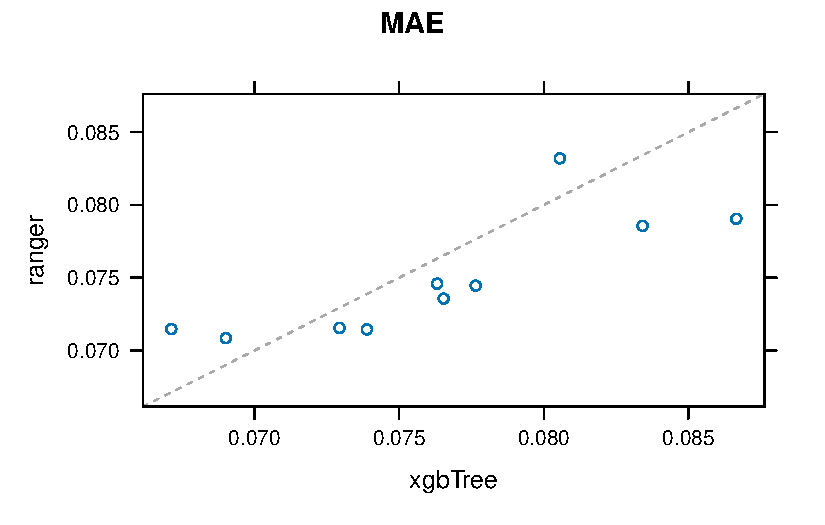
\includegraphics{MachineLearning_StaticPatterNN_Report_files/figure-pdf/final-models-comparison-1.pdf}

\begin{Shaded}
\begin{Highlighting}[]
\CommentTok{\# Plot comparison}
\FunctionTok{bwplot}\NormalTok{(resamples)}
\end{Highlighting}
\end{Shaded}

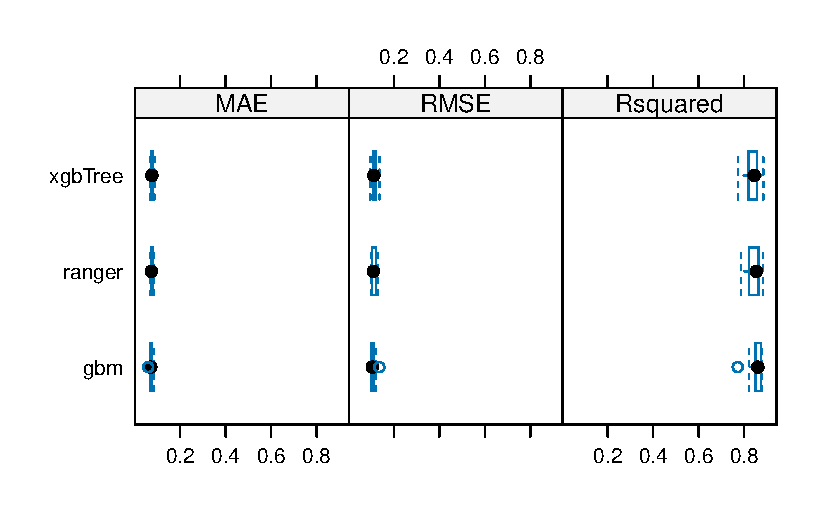
\includegraphics{MachineLearning_StaticPatterNN_Report_files/figure-pdf/final-models-comparison-2.pdf}

\begin{Shaded}
\begin{Highlighting}[]
\FunctionTok{save.image}\NormalTok{(}\StringTok{"./data/models.RData"}\NormalTok{)}
\FunctionTok{load}\NormalTok{(}\StringTok{"./data/models.RData"}\NormalTok{)}
\end{Highlighting}
\end{Shaded}

\subsubsection{Partial Dependence Plots}\label{partial-dependence-plots}

\begin{Shaded}
\begin{Highlighting}[]
\DocumentationTok{\#\# Partial dependence plots}
\CommentTok{\# Get all partial dependencies ==================}
\CommentTok{\# pp\_list\_ranger \textless{}{-} replicate(39, list())}
\CommentTok{\# for (var in seq\_along(1:length(names(dat\_train \%\textgreater{}\% select({-}Jaccard)))))\{}
\CommentTok{\#     pred\_var \textless{}{-} names(dat\_train \%\textgreater{}\% select({-}Jaccard))[var]}
\CommentTok{\#     pp\_list\_ranger[[var]] \textless{}{-} pdp::partial(}
\CommentTok{\#         rangerModel, }
\CommentTok{\#         pred.var = pred\_var, }
\CommentTok{\#         plot = FALSE)}
\CommentTok{\# \}}
\CommentTok{\# }
\CommentTok{\# }
\CommentTok{\# }
\CommentTok{\# pp\_list\_xgb \textless{}{-} replicate(39, list())}
\CommentTok{\# for (var in seq\_along(1:length(names(dat\_train \%\textgreater{}\% select({-}Jaccard)))))\{}
\CommentTok{\#     pred\_var \textless{}{-} names(dat\_train \%\textgreater{}\% select({-}Jaccard))[var]}
\CommentTok{\#     pp\_list\_xgb[[var]] \textless{}{-} partial(}
\CommentTok{\#         xgbModel, }
\CommentTok{\#         pred.var = pred\_var, }
\CommentTok{\#         plot = FALSE)}
\CommentTok{\# \}}
\CommentTok{\# }
\CommentTok{\# }
\CommentTok{\# }
\CommentTok{\# }
\CommentTok{\# pp\_list\_gbm \textless{}{-} replicate(39, list())}
\CommentTok{\# for (var in seq\_along(1:length(names(dat\_train \%\textgreater{}\% select({-}Jaccard)))))\{}
\CommentTok{\#     pred\_var \textless{}{-} names(dat\_train \%\textgreater{}\% select({-}Jaccard))[var]}
\CommentTok{\#     pp\_list\_gbm[[var]] \textless{}{-} partial(}
\CommentTok{\#         gbmModel, }
\CommentTok{\#         pred.var = pred\_var, }
\CommentTok{\#         plot = FALSE)}
\CommentTok{\# \}}
\CommentTok{\# }
\CommentTok{\# }
\CommentTok{\# pp\_list \textless{}{-} list(pp\_list\_ranger, pp\_list\_xgb, pp\_list\_gbm)}
\CommentTok{\#}
\CommentTok{\# saveRDS(pp\_list, "data/pp\_list.rds")}

\NormalTok{pp\_list }\OtherTok{\textless{}{-}} \FunctionTok{readRDS}\NormalTok{(}\StringTok{"./data/pp\_list.rds"}\NormalTok{)}
\NormalTok{pp\_list\_ranger }\OtherTok{\textless{}{-}}\NormalTok{ pp\_list[[}\DecValTok{1}\NormalTok{]]}
\NormalTok{pp\_list\_xgb }\OtherTok{\textless{}{-}}\NormalTok{ pp\_list[[}\DecValTok{2}\NormalTok{]]}
\NormalTok{pp\_list\_gbm }\OtherTok{\textless{}{-}}\NormalTok{ pp\_list[[}\DecValTok{3}\NormalTok{]]}


\DocumentationTok{\#\# Evaluate model =====}

\CommentTok{\# Plotting}

\CommentTok{\# Define the predictor names}
\NormalTok{predictors }\OtherTok{\textless{}{-}} \FunctionTok{names}\NormalTok{(dat\_train }\SpecialCharTok{\%\textgreater{}\%} \FunctionTok{select}\NormalTok{(}\SpecialCharTok{{-}}\NormalTok{Jaccard))}

\CommentTok{\# Initialize an empty list to store the plots}
\NormalTok{plots }\OtherTok{\textless{}{-}} \FunctionTok{list}\NormalTok{()}

\CommentTok{\# Function to determine if a column is categorical}
\NormalTok{is\_categorical }\OtherTok{\textless{}{-}} \ControlFlowTok{function}\NormalTok{(column) \{}
  \FunctionTok{is.factor}\NormalTok{(column) }\SpecialCharTok{||} \FunctionTok{is.character}\NormalTok{(column)}
\NormalTok{\}}

\CommentTok{\# Loop through the indices and create plots}
\ControlFlowTok{for}\NormalTok{ (i }\ControlFlowTok{in} \FunctionTok{seq\_along}\NormalTok{(}\DecValTok{1}\SpecialCharTok{:}\FunctionTok{length}\NormalTok{(predictors))) \{}
\NormalTok{  predictor }\OtherTok{\textless{}{-}} \FunctionTok{names}\NormalTok{(pp\_list\_ranger[[i]])[}\DecValTok{1}\NormalTok{]}
  
  \ControlFlowTok{if}\NormalTok{ (}\FunctionTok{is\_categorical}\NormalTok{(dat\_train[[predictor]])) \{}
    \CommentTok{\# Create boxplot for categorical predictors}
\NormalTok{    plots[[i]] }\OtherTok{\textless{}{-}} \FunctionTok{ggplot}\NormalTok{() }\SpecialCharTok{+}
      \FunctionTok{geom\_boxplot}\NormalTok{(}\AttributeTok{data =}\NormalTok{ pp\_list\_ranger[[i]], }\FunctionTok{aes}\NormalTok{(}\AttributeTok{x =}\NormalTok{ .data[[predictor]], }\AttributeTok{y =}\NormalTok{ yhat)) }\SpecialCharTok{+}
      \FunctionTok{geom\_boxplot}\NormalTok{(}\AttributeTok{data =}\NormalTok{ pp\_list\_xgb[[i]],}\FunctionTok{aes}\NormalTok{(}\AttributeTok{x =}\NormalTok{ .data[[predictor]], }\AttributeTok{y =}\NormalTok{ yhat), }\AttributeTok{linetype =} \StringTok{"dashed"}\NormalTok{) }\SpecialCharTok{+}
      \FunctionTok{geom\_boxplot}\NormalTok{(}\AttributeTok{data =}\NormalTok{ pp\_list\_gbm[[i]], }\FunctionTok{aes}\NormalTok{(}\AttributeTok{x =}\NormalTok{ .data[[predictor]], }\AttributeTok{y =}\NormalTok{ yhat), }\AttributeTok{linetype =} \StringTok{"dotted"}\NormalTok{) }\SpecialCharTok{+}
      \FunctionTok{labs}\NormalTok{(}\AttributeTok{x =} \FunctionTok{paste}\NormalTok{(predictor), }\AttributeTok{y =} \StringTok{"Partial Dependence"}\NormalTok{, }\AttributeTok{title =} \StringTok{"Partial Dependence Boxplots"}\NormalTok{) }\SpecialCharTok{+}
      \FunctionTok{theme\_bw}\NormalTok{() }\SpecialCharTok{+}
      \FunctionTok{ylim}\NormalTok{(}\DecValTok{0}\NormalTok{, }\DecValTok{1}\NormalTok{)}
\NormalTok{  \} }\ControlFlowTok{else}\NormalTok{ \{}
    \CommentTok{\# Create line plot for continuous predictors}
\NormalTok{    plots[[i]] }\OtherTok{\textless{}{-}} \FunctionTok{ggplot}\NormalTok{() }\SpecialCharTok{+}
      \FunctionTok{geom\_line}\NormalTok{(}\AttributeTok{data =}\NormalTok{ pp\_list\_ranger[[i]], }\FunctionTok{aes}\NormalTok{(}\AttributeTok{x =}\NormalTok{ .data[[predictor]], }\AttributeTok{y =}\NormalTok{ yhat)) }\SpecialCharTok{+}
      \FunctionTok{geom\_line}\NormalTok{(}\AttributeTok{data =}\NormalTok{ pp\_list\_xgb[[i]], }\FunctionTok{aes}\NormalTok{(}\AttributeTok{x =}\NormalTok{ .data[[predictor]], }\AttributeTok{y =}\NormalTok{ yhat), }\AttributeTok{linetype =} \StringTok{"dashed"}\NormalTok{) }\SpecialCharTok{+}
      \FunctionTok{geom\_line}\NormalTok{(}\AttributeTok{data =}\NormalTok{ pp\_list\_gbm[[i]], }\FunctionTok{aes}\NormalTok{(}\AttributeTok{x =}\NormalTok{ .data[[predictor]], }\AttributeTok{y =}\NormalTok{ yhat), }\AttributeTok{linetype =} \StringTok{"dotted"}\NormalTok{) }\SpecialCharTok{+}
      \FunctionTok{labs}\NormalTok{(}\AttributeTok{x =} \FunctionTok{paste}\NormalTok{(predictor), }\AttributeTok{y =} \StringTok{"Partial Dependence"}\NormalTok{, }\AttributeTok{title =} \StringTok{"Partial Dependence Plots"}\NormalTok{) }\SpecialCharTok{+}
      \FunctionTok{theme\_bw}\NormalTok{() }\SpecialCharTok{+}
      \FunctionTok{ylim}\NormalTok{(}\DecValTok{0}\NormalTok{, }\DecValTok{1}\NormalTok{)}
\NormalTok{  \}}
\NormalTok{\}}

\CommentTok{\# Arrange the plots in a grid}
\NormalTok{gridExtra}\SpecialCharTok{::}\FunctionTok{grid.arrange}\NormalTok{(}\AttributeTok{grobs =}\NormalTok{ plots, }\AttributeTok{ncol =} \DecValTok{6}\NormalTok{)}
\end{Highlighting}
\end{Shaded}

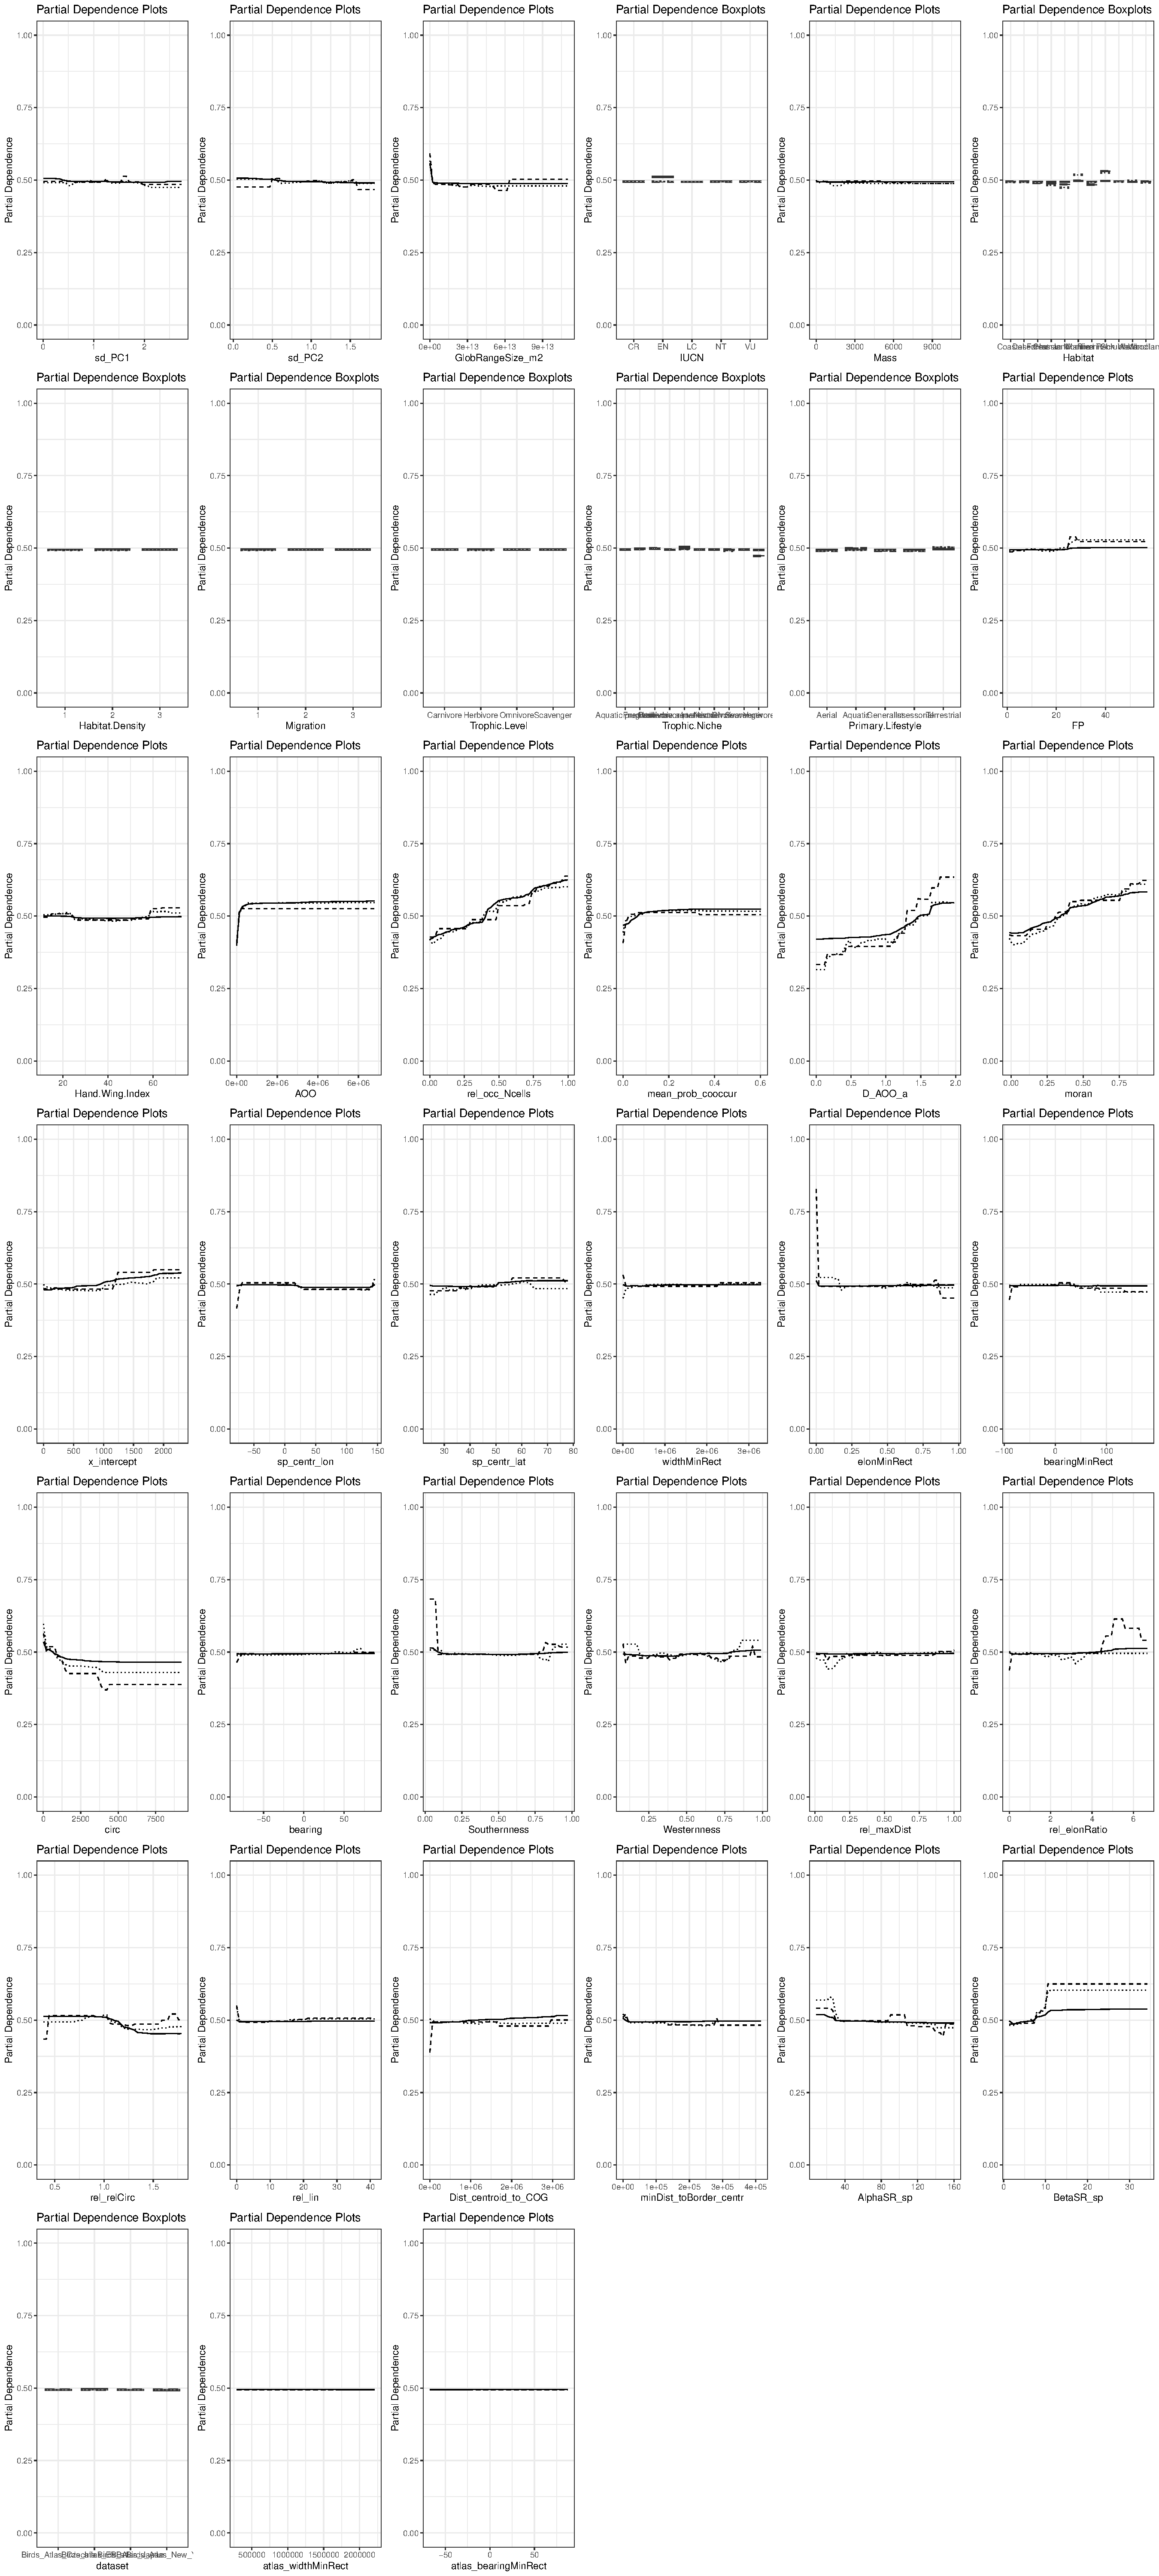
\includegraphics{MachineLearning_StaticPatterNN_Report_files/figure-pdf/partial-dependence-plots-1.pdf}

\subsubsection{Ensemble model}\label{ensemble-model}

Now we will compare randomForest to boosed regression trees or extreme
gradient boosting.

\begin{Shaded}
\begin{Highlighting}[]
\FunctionTok{set.seed}\NormalTok{(}\DecValTok{42}\NormalTok{)}
\NormalTok{trained\_control }\OtherTok{\textless{}{-}} \FunctionTok{trainControl}\NormalTok{(}
    \AttributeTok{method =} \StringTok{"repeatedcv"}\NormalTok{,}
    \AttributeTok{number =} \DecValTok{10}\NormalTok{,}
    \AttributeTok{repeats =} \DecValTok{3}\NormalTok{,}
    \AttributeTok{savePredictions =} \StringTok{"final"}\NormalTok{,}
    \AttributeTok{returnResamp =} \StringTok{"final"}\NormalTok{,}
    \AttributeTok{verboseIter =} \ConstantTok{TRUE}\NormalTok{,}
    \AttributeTok{index =}\NormalTok{ indices)}

\NormalTok{modelsList }\OtherTok{\textless{}{-}} \FunctionTok{caretList}\NormalTok{(}
\NormalTok{    Jaccard }\SpecialCharTok{\textasciitilde{}}\NormalTok{ .,}
    \AttributeTok{data =}\NormalTok{ dat\_train,}
    \AttributeTok{trControl =}\NormalTok{ trained\_control,}
    \AttributeTok{methodList =} \FunctionTok{c}\NormalTok{(}\StringTok{"gbm"}\NormalTok{, }\StringTok{"xgbTree"}\NormalTok{, }\StringTok{"ranger"}\NormalTok{),}
    \AttributeTok{tuneList =} \FunctionTok{list}\NormalTok{(}
      \AttributeTok{ranger =} \FunctionTok{caretModelSpec}\NormalTok{(}\AttributeTok{method =} \StringTok{"ranger"}\NormalTok{, }\AttributeTok{num.trees =} \DecValTok{1000}\NormalTok{, }\AttributeTok{importance =} \StringTok{"permutation"}\NormalTok{, }\AttributeTok{oob.error =} \ConstantTok{TRUE}\NormalTok{, }\AttributeTok{respect.unordered.factors =} \ConstantTok{TRUE}\NormalTok{ )}
\NormalTok{    ))}
\end{Highlighting}
\end{Shaded}

\begin{verbatim}
+ Resample01: mtry= 2, min.node.size=5, splitrule=variance 
- Resample01: mtry= 2, min.node.size=5, splitrule=variance 
+ Resample01: mtry=35, min.node.size=5, splitrule=variance 
- Resample01: mtry=35, min.node.size=5, splitrule=variance 
+ Resample01: mtry=68, min.node.size=5, splitrule=variance 
- Resample01: mtry=68, min.node.size=5, splitrule=variance 
+ Resample01: mtry= 2, min.node.size=5, splitrule=extratrees 
- Resample01: mtry= 2, min.node.size=5, splitrule=extratrees 
+ Resample01: mtry=35, min.node.size=5, splitrule=extratrees 
- Resample01: mtry=35, min.node.size=5, splitrule=extratrees 
+ Resample01: mtry=68, min.node.size=5, splitrule=extratrees 
- Resample01: mtry=68, min.node.size=5, splitrule=extratrees 
+ Resample02: mtry= 2, min.node.size=5, splitrule=variance 
- Resample02: mtry= 2, min.node.size=5, splitrule=variance 
+ Resample02: mtry=35, min.node.size=5, splitrule=variance 
- Resample02: mtry=35, min.node.size=5, splitrule=variance 
+ Resample02: mtry=68, min.node.size=5, splitrule=variance 
- Resample02: mtry=68, min.node.size=5, splitrule=variance 
+ Resample02: mtry= 2, min.node.size=5, splitrule=extratrees 
- Resample02: mtry= 2, min.node.size=5, splitrule=extratrees 
+ Resample02: mtry=35, min.node.size=5, splitrule=extratrees 
- Resample02: mtry=35, min.node.size=5, splitrule=extratrees 
+ Resample02: mtry=68, min.node.size=5, splitrule=extratrees 
- Resample02: mtry=68, min.node.size=5, splitrule=extratrees 
+ Resample03: mtry= 2, min.node.size=5, splitrule=variance 
- Resample03: mtry= 2, min.node.size=5, splitrule=variance 
+ Resample03: mtry=35, min.node.size=5, splitrule=variance 
- Resample03: mtry=35, min.node.size=5, splitrule=variance 
+ Resample03: mtry=68, min.node.size=5, splitrule=variance 
- Resample03: mtry=68, min.node.size=5, splitrule=variance 
+ Resample03: mtry= 2, min.node.size=5, splitrule=extratrees 
- Resample03: mtry= 2, min.node.size=5, splitrule=extratrees 
+ Resample03: mtry=35, min.node.size=5, splitrule=extratrees 
- Resample03: mtry=35, min.node.size=5, splitrule=extratrees 
+ Resample03: mtry=68, min.node.size=5, splitrule=extratrees 
- Resample03: mtry=68, min.node.size=5, splitrule=extratrees 
+ Resample04: mtry= 2, min.node.size=5, splitrule=variance 
- Resample04: mtry= 2, min.node.size=5, splitrule=variance 
+ Resample04: mtry=35, min.node.size=5, splitrule=variance 
- Resample04: mtry=35, min.node.size=5, splitrule=variance 
+ Resample04: mtry=68, min.node.size=5, splitrule=variance 
- Resample04: mtry=68, min.node.size=5, splitrule=variance 
+ Resample04: mtry= 2, min.node.size=5, splitrule=extratrees 
- Resample04: mtry= 2, min.node.size=5, splitrule=extratrees 
+ Resample04: mtry=35, min.node.size=5, splitrule=extratrees 
- Resample04: mtry=35, min.node.size=5, splitrule=extratrees 
+ Resample04: mtry=68, min.node.size=5, splitrule=extratrees 
- Resample04: mtry=68, min.node.size=5, splitrule=extratrees 
+ Resample05: mtry= 2, min.node.size=5, splitrule=variance 
- Resample05: mtry= 2, min.node.size=5, splitrule=variance 
+ Resample05: mtry=35, min.node.size=5, splitrule=variance 
- Resample05: mtry=35, min.node.size=5, splitrule=variance 
+ Resample05: mtry=68, min.node.size=5, splitrule=variance 
- Resample05: mtry=68, min.node.size=5, splitrule=variance 
+ Resample05: mtry= 2, min.node.size=5, splitrule=extratrees 
- Resample05: mtry= 2, min.node.size=5, splitrule=extratrees 
+ Resample05: mtry=35, min.node.size=5, splitrule=extratrees 
- Resample05: mtry=35, min.node.size=5, splitrule=extratrees 
+ Resample05: mtry=68, min.node.size=5, splitrule=extratrees 
- Resample05: mtry=68, min.node.size=5, splitrule=extratrees 
+ Resample06: mtry= 2, min.node.size=5, splitrule=variance 
- Resample06: mtry= 2, min.node.size=5, splitrule=variance 
+ Resample06: mtry=35, min.node.size=5, splitrule=variance 
- Resample06: mtry=35, min.node.size=5, splitrule=variance 
+ Resample06: mtry=68, min.node.size=5, splitrule=variance 
- Resample06: mtry=68, min.node.size=5, splitrule=variance 
+ Resample06: mtry= 2, min.node.size=5, splitrule=extratrees 
- Resample06: mtry= 2, min.node.size=5, splitrule=extratrees 
+ Resample06: mtry=35, min.node.size=5, splitrule=extratrees 
- Resample06: mtry=35, min.node.size=5, splitrule=extratrees 
+ Resample06: mtry=68, min.node.size=5, splitrule=extratrees 
- Resample06: mtry=68, min.node.size=5, splitrule=extratrees 
+ Resample07: mtry= 2, min.node.size=5, splitrule=variance 
- Resample07: mtry= 2, min.node.size=5, splitrule=variance 
+ Resample07: mtry=35, min.node.size=5, splitrule=variance 
- Resample07: mtry=35, min.node.size=5, splitrule=variance 
+ Resample07: mtry=68, min.node.size=5, splitrule=variance 
- Resample07: mtry=68, min.node.size=5, splitrule=variance 
+ Resample07: mtry= 2, min.node.size=5, splitrule=extratrees 
- Resample07: mtry= 2, min.node.size=5, splitrule=extratrees 
+ Resample07: mtry=35, min.node.size=5, splitrule=extratrees 
- Resample07: mtry=35, min.node.size=5, splitrule=extratrees 
+ Resample07: mtry=68, min.node.size=5, splitrule=extratrees 
- Resample07: mtry=68, min.node.size=5, splitrule=extratrees 
+ Resample08: mtry= 2, min.node.size=5, splitrule=variance 
- Resample08: mtry= 2, min.node.size=5, splitrule=variance 
+ Resample08: mtry=35, min.node.size=5, splitrule=variance 
- Resample08: mtry=35, min.node.size=5, splitrule=variance 
+ Resample08: mtry=68, min.node.size=5, splitrule=variance 
- Resample08: mtry=68, min.node.size=5, splitrule=variance 
+ Resample08: mtry= 2, min.node.size=5, splitrule=extratrees 
- Resample08: mtry= 2, min.node.size=5, splitrule=extratrees 
+ Resample08: mtry=35, min.node.size=5, splitrule=extratrees 
- Resample08: mtry=35, min.node.size=5, splitrule=extratrees 
+ Resample08: mtry=68, min.node.size=5, splitrule=extratrees 
- Resample08: mtry=68, min.node.size=5, splitrule=extratrees 
+ Resample09: mtry= 2, min.node.size=5, splitrule=variance 
- Resample09: mtry= 2, min.node.size=5, splitrule=variance 
+ Resample09: mtry=35, min.node.size=5, splitrule=variance 
- Resample09: mtry=35, min.node.size=5, splitrule=variance 
+ Resample09: mtry=68, min.node.size=5, splitrule=variance 
- Resample09: mtry=68, min.node.size=5, splitrule=variance 
+ Resample09: mtry= 2, min.node.size=5, splitrule=extratrees 
- Resample09: mtry= 2, min.node.size=5, splitrule=extratrees 
+ Resample09: mtry=35, min.node.size=5, splitrule=extratrees 
- Resample09: mtry=35, min.node.size=5, splitrule=extratrees 
+ Resample09: mtry=68, min.node.size=5, splitrule=extratrees 
- Resample09: mtry=68, min.node.size=5, splitrule=extratrees 
+ Resample10: mtry= 2, min.node.size=5, splitrule=variance 
- Resample10: mtry= 2, min.node.size=5, splitrule=variance 
+ Resample10: mtry=35, min.node.size=5, splitrule=variance 
- Resample10: mtry=35, min.node.size=5, splitrule=variance 
+ Resample10: mtry=68, min.node.size=5, splitrule=variance 
- Resample10: mtry=68, min.node.size=5, splitrule=variance 
+ Resample10: mtry= 2, min.node.size=5, splitrule=extratrees 
- Resample10: mtry= 2, min.node.size=5, splitrule=extratrees 
+ Resample10: mtry=35, min.node.size=5, splitrule=extratrees 
- Resample10: mtry=35, min.node.size=5, splitrule=extratrees 
+ Resample10: mtry=68, min.node.size=5, splitrule=extratrees 
- Resample10: mtry=68, min.node.size=5, splitrule=extratrees 
Aggregating results
Selecting tuning parameters
Fitting mtry = 68, splitrule = extratrees, min.node.size = 5 on full training set
+ Resample01: shrinkage=0.1, interaction.depth=1, n.minobsinnode=10, n.trees=150 
\end{verbatim}

\begin{verbatim}
Warning in (function (x, y, offset = NULL, misc = NULL, distribution =
"bernoulli", : variable 31: Trophic.NicheNectarivore has no variation.
\end{verbatim}

\begin{verbatim}
Iter   TrainDeviance   ValidDeviance   StepSize   Improve
     1        0.0731             nan     0.1000    0.0067
     2        0.0678             nan     0.1000    0.0051
     3        0.0627             nan     0.1000    0.0052
     4        0.0582             nan     0.1000    0.0045
     5        0.0545             nan     0.1000    0.0036
     6        0.0511             nan     0.1000    0.0033
     7        0.0485             nan     0.1000    0.0026
     8        0.0456             nan     0.1000    0.0027
     9        0.0430             nan     0.1000    0.0021
    10        0.0409             nan     0.1000    0.0020
    20        0.0304             nan     0.1000    0.0005
    40        0.0222             nan     0.1000    0.0002
    60        0.0181             nan     0.1000   -0.0000
    80        0.0155             nan     0.1000    0.0000
   100        0.0140             nan     0.1000   -0.0001
   120        0.0127             nan     0.1000   -0.0001
   140        0.0116             nan     0.1000    0.0000
   150        0.0113             nan     0.1000   -0.0001

- Resample01: shrinkage=0.1, interaction.depth=1, n.minobsinnode=10, n.trees=150 
+ Resample01: shrinkage=0.1, interaction.depth=2, n.minobsinnode=10, n.trees=150 
\end{verbatim}

\begin{verbatim}
Warning in (function (x, y, offset = NULL, misc = NULL, distribution =
"bernoulli", : variable 31: Trophic.NicheNectarivore has no variation.
\end{verbatim}

\begin{verbatim}
Iter   TrainDeviance   ValidDeviance   StepSize   Improve
     1        0.0701             nan     0.1000    0.0088
     2        0.0628             nan     0.1000    0.0071
     3        0.0567             nan     0.1000    0.0056
     4        0.0515             nan     0.1000    0.0046
     5        0.0471             nan     0.1000    0.0042
     6        0.0438             nan     0.1000    0.0030
     7        0.0407             nan     0.1000    0.0028
     8        0.0381             nan     0.1000    0.0025
     9        0.0360             nan     0.1000    0.0018
    10        0.0339             nan     0.1000    0.0021
    20        0.0216             nan     0.1000    0.0007
    40        0.0142             nan     0.1000   -0.0000
    60        0.0112             nan     0.1000    0.0001
    80        0.0094             nan     0.1000    0.0000
   100        0.0082             nan     0.1000    0.0000
   120        0.0074             nan     0.1000   -0.0000
   140        0.0067             nan     0.1000   -0.0000
   150        0.0065             nan     0.1000   -0.0001

- Resample01: shrinkage=0.1, interaction.depth=2, n.minobsinnode=10, n.trees=150 
+ Resample01: shrinkage=0.1, interaction.depth=3, n.minobsinnode=10, n.trees=150 
\end{verbatim}

\begin{verbatim}
Warning in (function (x, y, offset = NULL, misc = NULL, distribution =
"bernoulli", : variable 31: Trophic.NicheNectarivore has no variation.
\end{verbatim}

\begin{verbatim}
Iter   TrainDeviance   ValidDeviance   StepSize   Improve
     1        0.0707             nan     0.1000    0.0092
     2        0.0623             nan     0.1000    0.0083
     3        0.0561             nan     0.1000    0.0060
     4        0.0503             nan     0.1000    0.0055
     5        0.0454             nan     0.1000    0.0048
     6        0.0409             nan     0.1000    0.0043
     7        0.0373             nan     0.1000    0.0031
     8        0.0340             nan     0.1000    0.0031
     9        0.0311             nan     0.1000    0.0028
    10        0.0288             nan     0.1000    0.0020
    20        0.0168             nan     0.1000    0.0005
    40        0.0103             nan     0.1000   -0.0000
    60        0.0079             nan     0.1000    0.0000
    80        0.0067             nan     0.1000   -0.0001
   100        0.0059             nan     0.1000    0.0000
   120        0.0052             nan     0.1000   -0.0000
   140        0.0046             nan     0.1000   -0.0000
   150        0.0044             nan     0.1000   -0.0000

- Resample01: shrinkage=0.1, interaction.depth=3, n.minobsinnode=10, n.trees=150 
+ Resample02: shrinkage=0.1, interaction.depth=1, n.minobsinnode=10, n.trees=150 
\end{verbatim}

\begin{verbatim}
Warning in (function (x, y, offset = NULL, misc = NULL, distribution =
"bernoulli", : variable 9: HabitatDesert has no variation.
\end{verbatim}

\begin{verbatim}
Iter   TrainDeviance   ValidDeviance   StepSize   Improve
     1        0.0729             nan     0.1000    0.0061
     2        0.0675             nan     0.1000    0.0051
     3        0.0622             nan     0.1000    0.0051
     4        0.0580             nan     0.1000    0.0038
     5        0.0537             nan     0.1000    0.0042
     6        0.0503             nan     0.1000    0.0033
     7        0.0475             nan     0.1000    0.0028
     8        0.0449             nan     0.1000    0.0023
     9        0.0428             nan     0.1000    0.0020
    10        0.0410             nan     0.1000    0.0017
    20        0.0303             nan     0.1000    0.0006
    40        0.0217             nan     0.1000    0.0000
    60        0.0176             nan     0.1000    0.0001
    80        0.0150             nan     0.1000    0.0000
   100        0.0134             nan     0.1000   -0.0000
   120        0.0123             nan     0.1000   -0.0002
   140        0.0112             nan     0.1000   -0.0000
   150        0.0109             nan     0.1000   -0.0000

- Resample02: shrinkage=0.1, interaction.depth=1, n.minobsinnode=10, n.trees=150 
+ Resample02: shrinkage=0.1, interaction.depth=2, n.minobsinnode=10, n.trees=150 
\end{verbatim}

\begin{verbatim}
Warning in (function (x, y, offset = NULL, misc = NULL, distribution =
"bernoulli", : variable 9: HabitatDesert has no variation.
\end{verbatim}

\begin{verbatim}
Iter   TrainDeviance   ValidDeviance   StepSize   Improve
     1        0.0701             nan     0.1000    0.0091
     2        0.0631             nan     0.1000    0.0070
     3        0.0573             nan     0.1000    0.0057
     4        0.0520             nan     0.1000    0.0049
     5        0.0477             nan     0.1000    0.0042
     6        0.0432             nan     0.1000    0.0041
     7        0.0397             nan     0.1000    0.0032
     8        0.0371             nan     0.1000    0.0023
     9        0.0348             nan     0.1000    0.0020
    10        0.0325             nan     0.1000    0.0021
    20        0.0210             nan     0.1000    0.0005
    40        0.0135             nan     0.1000    0.0001
    60        0.0108             nan     0.1000   -0.0000
    80        0.0094             nan     0.1000   -0.0002
   100        0.0082             nan     0.1000   -0.0001
   120        0.0073             nan     0.1000   -0.0000
   140        0.0067             nan     0.1000   -0.0000
   150        0.0065             nan     0.1000   -0.0000

- Resample02: shrinkage=0.1, interaction.depth=2, n.minobsinnode=10, n.trees=150 
+ Resample02: shrinkage=0.1, interaction.depth=3, n.minobsinnode=10, n.trees=150 
\end{verbatim}

\begin{verbatim}
Warning in (function (x, y, offset = NULL, misc = NULL, distribution =
"bernoulli", : variable 9: HabitatDesert has no variation.
\end{verbatim}

\begin{verbatim}
Iter   TrainDeviance   ValidDeviance   StepSize   Improve
     1        0.0692             nan     0.1000    0.0095
     2        0.0617             nan     0.1000    0.0071
     3        0.0553             nan     0.1000    0.0061
     4        0.0489             nan     0.1000    0.0060
     5        0.0443             nan     0.1000    0.0045
     6        0.0400             nan     0.1000    0.0044
     7        0.0364             nan     0.1000    0.0032
     8        0.0332             nan     0.1000    0.0028
     9        0.0307             nan     0.1000    0.0023
    10        0.0285             nan     0.1000    0.0020
    20        0.0166             nan     0.1000    0.0003
    40        0.0103             nan     0.1000    0.0000
    60        0.0079             nan     0.1000   -0.0000
    80        0.0067             nan     0.1000   -0.0000
   100        0.0058             nan     0.1000   -0.0000
   120        0.0053             nan     0.1000   -0.0000
   140        0.0047             nan     0.1000   -0.0001
   150        0.0044             nan     0.1000   -0.0000

- Resample02: shrinkage=0.1, interaction.depth=3, n.minobsinnode=10, n.trees=150 
+ Resample03: shrinkage=0.1, interaction.depth=1, n.minobsinnode=10, n.trees=150 
Iter   TrainDeviance   ValidDeviance   StepSize   Improve
     1        0.0732             nan     0.1000    0.0068
     2        0.0675             nan     0.1000    0.0053
     3        0.0621             nan     0.1000    0.0052
     4        0.0578             nan     0.1000    0.0041
     5        0.0542             nan     0.1000    0.0036
     6        0.0509             nan     0.1000    0.0035
     7        0.0480             nan     0.1000    0.0027
     8        0.0451             nan     0.1000    0.0025
     9        0.0430             nan     0.1000    0.0020
    10        0.0413             nan     0.1000    0.0018
    20        0.0298             nan     0.1000    0.0003
    40        0.0204             nan     0.1000    0.0002
    60        0.0161             nan     0.1000    0.0001
    80        0.0138             nan     0.1000    0.0000
   100        0.0122             nan     0.1000   -0.0001
   120        0.0110             nan     0.1000    0.0000
   140        0.0101             nan     0.1000    0.0000
   150        0.0098             nan     0.1000    0.0000

- Resample03: shrinkage=0.1, interaction.depth=1, n.minobsinnode=10, n.trees=150 
+ Resample03: shrinkage=0.1, interaction.depth=2, n.minobsinnode=10, n.trees=150 
Iter   TrainDeviance   ValidDeviance   StepSize   Improve
     1        0.0720             nan     0.1000    0.0075
     2        0.0644             nan     0.1000    0.0076
     3        0.0574             nan     0.1000    0.0068
     4        0.0520             nan     0.1000    0.0051
     5        0.0470             nan     0.1000    0.0045
     6        0.0433             nan     0.1000    0.0036
     7        0.0402             nan     0.1000    0.0024
     8        0.0375             nan     0.1000    0.0024
     9        0.0349             nan     0.1000    0.0023
    10        0.0331             nan     0.1000    0.0015
    20        0.0200             nan     0.1000    0.0007
    40        0.0122             nan     0.1000    0.0001
    60        0.0094             nan     0.1000    0.0000
    80        0.0080             nan     0.1000   -0.0000
   100        0.0070             nan     0.1000   -0.0000
   120        0.0063             nan     0.1000   -0.0001
   140        0.0057             nan     0.1000   -0.0000
   150        0.0056             nan     0.1000   -0.0000

- Resample03: shrinkage=0.1, interaction.depth=2, n.minobsinnode=10, n.trees=150 
+ Resample03: shrinkage=0.1, interaction.depth=3, n.minobsinnode=10, n.trees=150 
Iter   TrainDeviance   ValidDeviance   StepSize   Improve
     1        0.0704             nan     0.1000    0.0097
     2        0.0624             nan     0.1000    0.0073
     3        0.0556             nan     0.1000    0.0066
     4        0.0499             nan     0.1000    0.0056
     5        0.0450             nan     0.1000    0.0047
     6        0.0404             nan     0.1000    0.0046
     7        0.0369             nan     0.1000    0.0033
     8        0.0343             nan     0.1000    0.0025
     9        0.0314             nan     0.1000    0.0026
    10        0.0290             nan     0.1000    0.0021
    20        0.0168             nan     0.1000    0.0002
    40        0.0097             nan     0.1000    0.0001
    60        0.0072             nan     0.1000   -0.0000
    80        0.0061             nan     0.1000   -0.0001
   100        0.0053             nan     0.1000   -0.0001
   120        0.0046             nan     0.1000   -0.0000
   140        0.0040             nan     0.1000   -0.0000
   150        0.0038             nan     0.1000   -0.0000

- Resample03: shrinkage=0.1, interaction.depth=3, n.minobsinnode=10, n.trees=150 
+ Resample04: shrinkage=0.1, interaction.depth=1, n.minobsinnode=10, n.trees=150 
\end{verbatim}

\begin{verbatim}
Warning in (function (x, y, offset = NULL, misc = NULL, distribution =
"bernoulli", : variable 9: HabitatDesert has no variation.
\end{verbatim}

\begin{verbatim}
Iter   TrainDeviance   ValidDeviance   StepSize   Improve
     1        0.0736             nan     0.1000    0.0064
     2        0.0677             nan     0.1000    0.0055
     3        0.0625             nan     0.1000    0.0049
     4        0.0585             nan     0.1000    0.0041
     5        0.0550             nan     0.1000    0.0037
     6        0.0517             nan     0.1000    0.0031
     7        0.0490             nan     0.1000    0.0028
     8        0.0465             nan     0.1000    0.0025
     9        0.0444             nan     0.1000    0.0019
    10        0.0423             nan     0.1000    0.0017
    20        0.0317             nan     0.1000    0.0006
    40        0.0229             nan     0.1000    0.0000
    60        0.0183             nan     0.1000   -0.0000
    80        0.0158             nan     0.1000   -0.0001
   100        0.0141             nan     0.1000   -0.0000
   120        0.0128             nan     0.1000   -0.0001
   140        0.0117             nan     0.1000   -0.0001
   150        0.0114             nan     0.1000   -0.0001

- Resample04: shrinkage=0.1, interaction.depth=1, n.minobsinnode=10, n.trees=150 
+ Resample04: shrinkage=0.1, interaction.depth=2, n.minobsinnode=10, n.trees=150 
\end{verbatim}

\begin{verbatim}
Warning in (function (x, y, offset = NULL, misc = NULL, distribution =
"bernoulli", : variable 9: HabitatDesert has no variation.
\end{verbatim}

\begin{verbatim}
Iter   TrainDeviance   ValidDeviance   StepSize   Improve
     1        0.0715             nan     0.1000    0.0079
     2        0.0647             nan     0.1000    0.0067
     3        0.0582             nan     0.1000    0.0066
     4        0.0529             nan     0.1000    0.0048
     5        0.0482             nan     0.1000    0.0046
     6        0.0447             nan     0.1000    0.0033
     7        0.0411             nan     0.1000    0.0035
     8        0.0383             nan     0.1000    0.0026
     9        0.0359             nan     0.1000    0.0020
    10        0.0336             nan     0.1000    0.0021
    20        0.0217             nan     0.1000    0.0006
    40        0.0145             nan     0.1000    0.0000
    60        0.0114             nan     0.1000   -0.0001
    80        0.0097             nan     0.1000   -0.0001
   100        0.0086             nan     0.1000   -0.0000
   120        0.0077             nan     0.1000   -0.0000
   140        0.0070             nan     0.1000   -0.0001
   150        0.0067             nan     0.1000   -0.0000

- Resample04: shrinkage=0.1, interaction.depth=2, n.minobsinnode=10, n.trees=150 
+ Resample04: shrinkage=0.1, interaction.depth=3, n.minobsinnode=10, n.trees=150 
\end{verbatim}

\begin{verbatim}
Warning in (function (x, y, offset = NULL, misc = NULL, distribution =
"bernoulli", : variable 9: HabitatDesert has no variation.
\end{verbatim}

\begin{verbatim}
Iter   TrainDeviance   ValidDeviance   StepSize   Improve
     1        0.0704             nan     0.1000    0.0086
     2        0.0630             nan     0.1000    0.0068
     3        0.0566             nan     0.1000    0.0061
     4        0.0506             nan     0.1000    0.0055
     5        0.0455             nan     0.1000    0.0047
     6        0.0413             nan     0.1000    0.0038
     7        0.0376             nan     0.1000    0.0034
     8        0.0349             nan     0.1000    0.0024
     9        0.0323             nan     0.1000    0.0022
    10        0.0300             nan     0.1000    0.0022
    20        0.0181             nan     0.1000    0.0002
    40        0.0117             nan     0.1000   -0.0000
    60        0.0090             nan     0.1000    0.0000
    80        0.0075             nan     0.1000   -0.0001
   100        0.0064             nan     0.1000   -0.0000
   120        0.0055             nan     0.1000   -0.0001
   140        0.0048             nan     0.1000   -0.0000
   150        0.0046             nan     0.1000   -0.0000

- Resample04: shrinkage=0.1, interaction.depth=3, n.minobsinnode=10, n.trees=150 
+ Resample05: shrinkage=0.1, interaction.depth=1, n.minobsinnode=10, n.trees=150 
Iter   TrainDeviance   ValidDeviance   StepSize   Improve
     1        0.0745             nan     0.1000    0.0064
     2        0.0685             nan     0.1000    0.0062
     3        0.0632             nan     0.1000    0.0052
     4        0.0590             nan     0.1000    0.0043
     5        0.0550             nan     0.1000    0.0036
     6        0.0520             nan     0.1000    0.0033
     7        0.0491             nan     0.1000    0.0029
     8        0.0466             nan     0.1000    0.0026
     9        0.0446             nan     0.1000    0.0020
    10        0.0424             nan     0.1000    0.0020
    20        0.0310             nan     0.1000    0.0007
    40        0.0224             nan     0.1000   -0.0000
    60        0.0181             nan     0.1000    0.0001
    80        0.0157             nan     0.1000   -0.0001
   100        0.0141             nan     0.1000   -0.0000
   120        0.0129             nan     0.1000   -0.0001
   140        0.0119             nan     0.1000   -0.0000
   150        0.0115             nan     0.1000    0.0000

- Resample05: shrinkage=0.1, interaction.depth=1, n.minobsinnode=10, n.trees=150 
+ Resample05: shrinkage=0.1, interaction.depth=2, n.minobsinnode=10, n.trees=150 
Iter   TrainDeviance   ValidDeviance   StepSize   Improve
     1        0.0726             nan     0.1000    0.0078
     2        0.0649             nan     0.1000    0.0078
     3        0.0579             nan     0.1000    0.0072
     4        0.0527             nan     0.1000    0.0049
     5        0.0477             nan     0.1000    0.0045
     6        0.0440             nan     0.1000    0.0038
     7        0.0405             nan     0.1000    0.0031
     8        0.0378             nan     0.1000    0.0023
     9        0.0350             nan     0.1000    0.0025
    10        0.0330             nan     0.1000    0.0017
    20        0.0210             nan     0.1000    0.0004
    40        0.0137             nan     0.1000    0.0001
    60        0.0106             nan     0.1000    0.0001
    80        0.0090             nan     0.1000   -0.0000
   100        0.0077             nan     0.1000    0.0000
   120        0.0068             nan     0.1000   -0.0000
   140        0.0062             nan     0.1000   -0.0000
   150        0.0060             nan     0.1000   -0.0001

- Resample05: shrinkage=0.1, interaction.depth=2, n.minobsinnode=10, n.trees=150 
+ Resample05: shrinkage=0.1, interaction.depth=3, n.minobsinnode=10, n.trees=150 
Iter   TrainDeviance   ValidDeviance   StepSize   Improve
     1        0.0716             nan     0.1000    0.0087
     2        0.0631             nan     0.1000    0.0081
     3        0.0557             nan     0.1000    0.0066
     4        0.0497             nan     0.1000    0.0059
     5        0.0448             nan     0.1000    0.0046
     6        0.0409             nan     0.1000    0.0038
     7        0.0375             nan     0.1000    0.0031
     8        0.0345             nan     0.1000    0.0028
     9        0.0317             nan     0.1000    0.0024
    10        0.0294             nan     0.1000    0.0018
    20        0.0175             nan     0.1000    0.0006
    40        0.0106             nan     0.1000    0.0000
    60        0.0081             nan     0.1000   -0.0000
    80        0.0067             nan     0.1000   -0.0000
   100        0.0057             nan     0.1000   -0.0000
   120        0.0050             nan     0.1000   -0.0000
   140        0.0044             nan     0.1000   -0.0000
   150        0.0042             nan     0.1000   -0.0000

- Resample05: shrinkage=0.1, interaction.depth=3, n.minobsinnode=10, n.trees=150 
+ Resample06: shrinkage=0.1, interaction.depth=1, n.minobsinnode=10, n.trees=150 
Iter   TrainDeviance   ValidDeviance   StepSize   Improve
     1        0.0736             nan     0.1000    0.0068
     2        0.0677             nan     0.1000    0.0053
     3        0.0626             nan     0.1000    0.0051
     4        0.0581             nan     0.1000    0.0044
     5        0.0545             nan     0.1000    0.0032
     6        0.0510             nan     0.1000    0.0035
     7        0.0483             nan     0.1000    0.0023
     8        0.0456             nan     0.1000    0.0023
     9        0.0431             nan     0.1000    0.0024
    10        0.0413             nan     0.1000    0.0017
    20        0.0296             nan     0.1000    0.0008
    40        0.0219             nan     0.1000    0.0002
    60        0.0179             nan     0.1000   -0.0000
    80        0.0156             nan     0.1000   -0.0001
   100        0.0138             nan     0.1000    0.0000
   120        0.0126             nan     0.1000   -0.0000
   140        0.0120             nan     0.1000   -0.0001
   150        0.0117             nan     0.1000   -0.0000

- Resample06: shrinkage=0.1, interaction.depth=1, n.minobsinnode=10, n.trees=150 
+ Resample06: shrinkage=0.1, interaction.depth=2, n.minobsinnode=10, n.trees=150 
Iter   TrainDeviance   ValidDeviance   StepSize   Improve
     1        0.0722             nan     0.1000    0.0077
     2        0.0645             nan     0.1000    0.0075
     3        0.0582             nan     0.1000    0.0062
     4        0.0531             nan     0.1000    0.0052
     5        0.0488             nan     0.1000    0.0043
     6        0.0443             nan     0.1000    0.0040
     7        0.0409             nan     0.1000    0.0027
     8        0.0382             nan     0.1000    0.0025
     9        0.0357             nan     0.1000    0.0019
    10        0.0331             nan     0.1000    0.0022
    20        0.0213             nan     0.1000    0.0007
    40        0.0141             nan     0.1000   -0.0004
    60        0.0111             nan     0.1000   -0.0001
    80        0.0094             nan     0.1000    0.0000
   100        0.0083             nan     0.1000   -0.0001
   120        0.0074             nan     0.1000   -0.0001
   140        0.0068             nan     0.1000   -0.0001
   150        0.0065             nan     0.1000   -0.0000

- Resample06: shrinkage=0.1, interaction.depth=2, n.minobsinnode=10, n.trees=150 
+ Resample06: shrinkage=0.1, interaction.depth=3, n.minobsinnode=10, n.trees=150 
Iter   TrainDeviance   ValidDeviance   StepSize   Improve
     1        0.0711             nan     0.1000    0.0084
     2        0.0628             nan     0.1000    0.0081
     3        0.0562             nan     0.1000    0.0063
     4        0.0506             nan     0.1000    0.0056
     5        0.0455             nan     0.1000    0.0047
     6        0.0411             nan     0.1000    0.0040
     7        0.0377             nan     0.1000    0.0031
     8        0.0344             nan     0.1000    0.0031
     9        0.0320             nan     0.1000    0.0019
    10        0.0297             nan     0.1000    0.0020
    20        0.0174             nan     0.1000    0.0004
    40        0.0108             nan     0.1000    0.0000
    60        0.0084             nan     0.1000   -0.0000
    80        0.0070             nan     0.1000   -0.0001
   100        0.0061             nan     0.1000   -0.0001
   120        0.0052             nan     0.1000   -0.0001
   140        0.0047             nan     0.1000   -0.0000
   150        0.0044             nan     0.1000   -0.0000

- Resample06: shrinkage=0.1, interaction.depth=3, n.minobsinnode=10, n.trees=150 
+ Resample07: shrinkage=0.1, interaction.depth=1, n.minobsinnode=10, n.trees=150 
Iter   TrainDeviance   ValidDeviance   StepSize   Improve
     1        0.0729             nan     0.1000    0.0062
     2        0.0675             nan     0.1000    0.0050
     3        0.0623             nan     0.1000    0.0049
     4        0.0579             nan     0.1000    0.0043
     5        0.0542             nan     0.1000    0.0035
     6        0.0511             nan     0.1000    0.0030
     7        0.0481             nan     0.1000    0.0027
     8        0.0459             nan     0.1000    0.0021
     9        0.0439             nan     0.1000    0.0017
    10        0.0419             nan     0.1000    0.0020
    20        0.0305             nan     0.1000    0.0007
    40        0.0212             nan     0.1000   -0.0000
    60        0.0172             nan     0.1000    0.0001
    80        0.0148             nan     0.1000   -0.0002
   100        0.0131             nan     0.1000    0.0001
   120        0.0118             nan     0.1000   -0.0000
   140        0.0109             nan     0.1000   -0.0000
   150        0.0104             nan     0.1000    0.0000

- Resample07: shrinkage=0.1, interaction.depth=1, n.minobsinnode=10, n.trees=150 
+ Resample07: shrinkage=0.1, interaction.depth=2, n.minobsinnode=10, n.trees=150 
Iter   TrainDeviance   ValidDeviance   StepSize   Improve
     1        0.0711             nan     0.1000    0.0083
     2        0.0637             nan     0.1000    0.0070
     3        0.0582             nan     0.1000    0.0055
     4        0.0524             nan     0.1000    0.0058
     5        0.0476             nan     0.1000    0.0047
     6        0.0441             nan     0.1000    0.0032
     7        0.0407             nan     0.1000    0.0033
     8        0.0377             nan     0.1000    0.0027
     9        0.0350             nan     0.1000    0.0025
    10        0.0330             nan     0.1000    0.0018
    20        0.0211             nan     0.1000    0.0003
    40        0.0130             nan     0.1000    0.0001
    60        0.0102             nan     0.1000   -0.0001
    80        0.0087             nan     0.1000    0.0000
   100        0.0076             nan     0.1000   -0.0001
   120        0.0069             nan     0.1000   -0.0000
   140        0.0061             nan     0.1000    0.0000
   150        0.0058             nan     0.1000   -0.0000

- Resample07: shrinkage=0.1, interaction.depth=2, n.minobsinnode=10, n.trees=150 
+ Resample07: shrinkage=0.1, interaction.depth=3, n.minobsinnode=10, n.trees=150 
Iter   TrainDeviance   ValidDeviance   StepSize   Improve
     1        0.0701             nan     0.1000    0.0083
     2        0.0619             nan     0.1000    0.0073
     3        0.0555             nan     0.1000    0.0062
     4        0.0497             nan     0.1000    0.0059
     5        0.0450             nan     0.1000    0.0045
     6        0.0404             nan     0.1000    0.0042
     7        0.0370             nan     0.1000    0.0033
     8        0.0341             nan     0.1000    0.0027
     9        0.0311             nan     0.1000    0.0029
    10        0.0288             nan     0.1000    0.0020
    20        0.0167             nan     0.1000    0.0005
    40        0.0101             nan     0.1000    0.0001
    60        0.0077             nan     0.1000   -0.0000
    80        0.0064             nan     0.1000    0.0000
   100        0.0054             nan     0.1000   -0.0000
   120        0.0048             nan     0.1000   -0.0000
   140        0.0042             nan     0.1000   -0.0000
   150        0.0040             nan     0.1000   -0.0000

- Resample07: shrinkage=0.1, interaction.depth=3, n.minobsinnode=10, n.trees=150 
+ Resample08: shrinkage=0.1, interaction.depth=1, n.minobsinnode=10, n.trees=150 
Iter   TrainDeviance   ValidDeviance   StepSize   Improve
     1        0.0728             nan     0.1000    0.0058
     2        0.0669             nan     0.1000    0.0060
     3        0.0618             nan     0.1000    0.0047
     4        0.0574             nan     0.1000    0.0044
     5        0.0538             nan     0.1000    0.0035
     6        0.0506             nan     0.1000    0.0031
     7        0.0480             nan     0.1000    0.0024
     8        0.0454             nan     0.1000    0.0026
     9        0.0431             nan     0.1000    0.0020
    10        0.0412             nan     0.1000    0.0018
    20        0.0303             nan     0.1000    0.0007
    40        0.0216             nan     0.1000    0.0001
    60        0.0174             nan     0.1000   -0.0000
    80        0.0149             nan     0.1000   -0.0000
   100        0.0132             nan     0.1000    0.0000
   120        0.0121             nan     0.1000    0.0000
   140        0.0112             nan     0.1000   -0.0001
   150        0.0108             nan     0.1000   -0.0000

- Resample08: shrinkage=0.1, interaction.depth=1, n.minobsinnode=10, n.trees=150 
+ Resample08: shrinkage=0.1, interaction.depth=2, n.minobsinnode=10, n.trees=150 
Iter   TrainDeviance   ValidDeviance   StepSize   Improve
     1        0.0706             nan     0.1000    0.0085
     2        0.0636             nan     0.1000    0.0069
     3        0.0569             nan     0.1000    0.0063
     4        0.0518             nan     0.1000    0.0046
     5        0.0475             nan     0.1000    0.0042
     6        0.0436             nan     0.1000    0.0035
     7        0.0403             nan     0.1000    0.0032
     8        0.0373             nan     0.1000    0.0027
     9        0.0350             nan     0.1000    0.0020
    10        0.0333             nan     0.1000    0.0015
    20        0.0214             nan     0.1000    0.0006
    40        0.0140             nan     0.1000    0.0002
    60        0.0110             nan     0.1000   -0.0001
    80        0.0091             nan     0.1000   -0.0000
   100        0.0078             nan     0.1000    0.0000
   120        0.0070             nan     0.1000   -0.0000
   140        0.0063             nan     0.1000   -0.0000
   150        0.0061             nan     0.1000   -0.0000

- Resample08: shrinkage=0.1, interaction.depth=2, n.minobsinnode=10, n.trees=150 
+ Resample08: shrinkage=0.1, interaction.depth=3, n.minobsinnode=10, n.trees=150 
Iter   TrainDeviance   ValidDeviance   StepSize   Improve
     1        0.0698             nan     0.1000    0.0092
     2        0.0621             nan     0.1000    0.0075
     3        0.0556             nan     0.1000    0.0069
     4        0.0497             nan     0.1000    0.0060
     5        0.0447             nan     0.1000    0.0048
     6        0.0404             nan     0.1000    0.0041
     7        0.0372             nan     0.1000    0.0027
     8        0.0342             nan     0.1000    0.0029
     9        0.0316             nan     0.1000    0.0022
    10        0.0293             nan     0.1000    0.0021
    20        0.0168             nan     0.1000    0.0005
    40        0.0102             nan     0.1000   -0.0001
    60        0.0077             nan     0.1000    0.0000
    80        0.0063             nan     0.1000   -0.0000
   100        0.0054             nan     0.1000   -0.0000
   120        0.0047             nan     0.1000   -0.0000
   140        0.0042             nan     0.1000   -0.0000
   150        0.0040             nan     0.1000   -0.0000

- Resample08: shrinkage=0.1, interaction.depth=3, n.minobsinnode=10, n.trees=150 
+ Resample09: shrinkage=0.1, interaction.depth=1, n.minobsinnode=10, n.trees=150 
Iter   TrainDeviance   ValidDeviance   StepSize   Improve
     1        0.0728             nan     0.1000    0.0065
     2        0.0667             nan     0.1000    0.0059
     3        0.0611             nan     0.1000    0.0049
     4        0.0569             nan     0.1000    0.0043
     5        0.0530             nan     0.1000    0.0036
     6        0.0497             nan     0.1000    0.0032
     7        0.0468             nan     0.1000    0.0028
     8        0.0443             nan     0.1000    0.0025
     9        0.0422             nan     0.1000    0.0020
    10        0.0401             nan     0.1000    0.0019
    20        0.0295             nan     0.1000    0.0007
    40        0.0207             nan     0.1000    0.0003
    60        0.0167             nan     0.1000    0.0001
    80        0.0144             nan     0.1000   -0.0000
   100        0.0129             nan     0.1000    0.0000
   120        0.0117             nan     0.1000   -0.0000
   140        0.0110             nan     0.1000    0.0000
   150        0.0106             nan     0.1000   -0.0000

- Resample09: shrinkage=0.1, interaction.depth=1, n.minobsinnode=10, n.trees=150 
+ Resample09: shrinkage=0.1, interaction.depth=2, n.minobsinnode=10, n.trees=150 
Iter   TrainDeviance   ValidDeviance   StepSize   Improve
     1        0.0708             nan     0.1000    0.0095
     2        0.0630             nan     0.1000    0.0071
     3        0.0566             nan     0.1000    0.0066
     4        0.0516             nan     0.1000    0.0051
     5        0.0470             nan     0.1000    0.0047
     6        0.0433             nan     0.1000    0.0036
     7        0.0399             nan     0.1000    0.0031
     8        0.0370             nan     0.1000    0.0029
     9        0.0347             nan     0.1000    0.0021
    10        0.0325             nan     0.1000    0.0019
    20        0.0206             nan     0.1000    0.0005
    40        0.0131             nan     0.1000    0.0000
    60        0.0105             nan     0.1000   -0.0000
    80        0.0089             nan     0.1000   -0.0001
   100        0.0079             nan     0.1000   -0.0000
   120        0.0070             nan     0.1000   -0.0000
   140        0.0065             nan     0.1000   -0.0000
   150        0.0061             nan     0.1000   -0.0000

- Resample09: shrinkage=0.1, interaction.depth=2, n.minobsinnode=10, n.trees=150 
+ Resample09: shrinkage=0.1, interaction.depth=3, n.minobsinnode=10, n.trees=150 
Iter   TrainDeviance   ValidDeviance   StepSize   Improve
     1        0.0698             nan     0.1000    0.0096
     2        0.0613             nan     0.1000    0.0080
     3        0.0550             nan     0.1000    0.0054
     4        0.0494             nan     0.1000    0.0055
     5        0.0446             nan     0.1000    0.0042
     6        0.0406             nan     0.1000    0.0039
     7        0.0373             nan     0.1000    0.0031
     8        0.0339             nan     0.1000    0.0029
     9        0.0314             nan     0.1000    0.0022
    10        0.0289             nan     0.1000    0.0021
    20        0.0167             nan     0.1000    0.0002
    40        0.0103             nan     0.1000   -0.0000
    60        0.0078             nan     0.1000    0.0000
    80        0.0064             nan     0.1000   -0.0000
   100        0.0055             nan     0.1000   -0.0000
   120        0.0048             nan     0.1000   -0.0000
   140        0.0043             nan     0.1000   -0.0000
   150        0.0041             nan     0.1000   -0.0000

- Resample09: shrinkage=0.1, interaction.depth=3, n.minobsinnode=10, n.trees=150 
+ Resample10: shrinkage=0.1, interaction.depth=1, n.minobsinnode=10, n.trees=150 
\end{verbatim}

\begin{verbatim}
Warning in (function (x, y, offset = NULL, misc = NULL, distribution =
"bernoulli", : variable 9: HabitatDesert has no variation.
\end{verbatim}

\begin{verbatim}
Iter   TrainDeviance   ValidDeviance   StepSize   Improve
     1        0.0739             nan     0.1000    0.0062
     2        0.0680             nan     0.1000    0.0057
     3        0.0635             nan     0.1000    0.0049
     4        0.0590             nan     0.1000    0.0042
     5        0.0556             nan     0.1000    0.0034
     6        0.0525             nan     0.1000    0.0030
     7        0.0496             nan     0.1000    0.0026
     8        0.0470             nan     0.1000    0.0025
     9        0.0447             nan     0.1000    0.0020
    10        0.0427             nan     0.1000    0.0020
    20        0.0320             nan     0.1000    0.0006
    40        0.0224             nan     0.1000    0.0001
    60        0.0180             nan     0.1000    0.0000
    80        0.0156             nan     0.1000   -0.0000
   100        0.0137             nan     0.1000   -0.0001
   120        0.0126             nan     0.1000    0.0000
   140        0.0117             nan     0.1000   -0.0000
   150        0.0113             nan     0.1000    0.0000

- Resample10: shrinkage=0.1, interaction.depth=1, n.minobsinnode=10, n.trees=150 
+ Resample10: shrinkage=0.1, interaction.depth=2, n.minobsinnode=10, n.trees=150 
\end{verbatim}

\begin{verbatim}
Warning in (function (x, y, offset = NULL, misc = NULL, distribution =
"bernoulli", : variable 9: HabitatDesert has no variation.
\end{verbatim}

\begin{verbatim}
Iter   TrainDeviance   ValidDeviance   StepSize   Improve
     1        0.0711             nan     0.1000    0.0088
     2        0.0643             nan     0.1000    0.0064
     3        0.0583             nan     0.1000    0.0058
     4        0.0534             nan     0.1000    0.0047
     5        0.0498             nan     0.1000    0.0030
     6        0.0462             nan     0.1000    0.0029
     7        0.0433             nan     0.1000    0.0024
     8        0.0396             nan     0.1000    0.0034
     9        0.0374             nan     0.1000    0.0020
    10        0.0352             nan     0.1000    0.0016
    20        0.0209             nan     0.1000    0.0004
    40        0.0137             nan     0.1000    0.0001
    60        0.0110             nan     0.1000   -0.0000
    80        0.0094             nan     0.1000    0.0000
   100        0.0082             nan     0.1000    0.0000
   120        0.0075             nan     0.1000   -0.0001
   140        0.0068             nan     0.1000   -0.0000
   150        0.0065             nan     0.1000   -0.0001

- Resample10: shrinkage=0.1, interaction.depth=2, n.minobsinnode=10, n.trees=150 
+ Resample10: shrinkage=0.1, interaction.depth=3, n.minobsinnode=10, n.trees=150 
\end{verbatim}

\begin{verbatim}
Warning in (function (x, y, offset = NULL, misc = NULL, distribution =
"bernoulli", : variable 9: HabitatDesert has no variation.
\end{verbatim}

\begin{verbatim}
Iter   TrainDeviance   ValidDeviance   StepSize   Improve
     1        0.0708             nan     0.1000    0.0089
     2        0.0629             nan     0.1000    0.0075
     3        0.0560             nan     0.1000    0.0064
     4        0.0503             nan     0.1000    0.0051
     5        0.0453             nan     0.1000    0.0043
     6        0.0414             nan     0.1000    0.0029
     7        0.0375             nan     0.1000    0.0037
     8        0.0345             nan     0.1000    0.0027
     9        0.0320             nan     0.1000    0.0020
    10        0.0300             nan     0.1000    0.0018
    20        0.0172             nan     0.1000    0.0006
    40        0.0107             nan     0.1000    0.0000
    60        0.0082             nan     0.1000   -0.0001
    80        0.0068             nan     0.1000   -0.0000
   100        0.0058             nan     0.1000   -0.0001
   120        0.0051             nan     0.1000   -0.0000
   140        0.0046             nan     0.1000   -0.0000
   150        0.0044             nan     0.1000   -0.0001

- Resample10: shrinkage=0.1, interaction.depth=3, n.minobsinnode=10, n.trees=150 
Aggregating results
Selecting tuning parameters
Fitting n.trees = 150, interaction.depth = 3, shrinkage = 0.1, n.minobsinnode = 10 on full training set
Iter   TrainDeviance   ValidDeviance   StepSize   Improve
     1        0.0705             nan     0.1000    0.0094
     2        0.0627             nan     0.1000    0.0071
     3        0.0564             nan     0.1000    0.0061
     4        0.0501             nan     0.1000    0.0062
     5        0.0451             nan     0.1000    0.0046
     6        0.0407             nan     0.1000    0.0041
     7        0.0369             nan     0.1000    0.0036
     8        0.0338             nan     0.1000    0.0026
     9        0.0314             nan     0.1000    0.0025
    10        0.0290             nan     0.1000    0.0022
    20        0.0170             nan     0.1000    0.0004
    40        0.0109             nan     0.1000   -0.0000
    60        0.0087             nan     0.1000   -0.0001
    80        0.0075             nan     0.1000   -0.0000
   100        0.0066             nan     0.1000   -0.0000
   120        0.0058             nan     0.1000   -0.0001
   140        0.0052             nan     0.1000   -0.0000
   150        0.0049             nan     0.1000   -0.0000

+ Resample01: eta=0.3, max_depth=1, gamma=0, colsample_bytree=0.6, min_child_weight=1, subsample=0.50, nrounds=150 
[15:31:58] WARNING: src/c_api/c_api.cc:935: `ntree_limit` is deprecated, use `iteration_range` instead.
[15:31:58] WARNING: src/c_api/c_api.cc:935: `ntree_limit` is deprecated, use `iteration_range` instead.
- Resample01: eta=0.3, max_depth=1, gamma=0, colsample_bytree=0.6, min_child_weight=1, subsample=0.50, nrounds=150 
+ Resample01: eta=0.3, max_depth=1, gamma=0, colsample_bytree=0.6, min_child_weight=1, subsample=0.75, nrounds=150 
[15:31:59] WARNING: src/c_api/c_api.cc:935: `ntree_limit` is deprecated, use `iteration_range` instead.
[15:31:59] WARNING: src/c_api/c_api.cc:935: `ntree_limit` is deprecated, use `iteration_range` instead.
- Resample01: eta=0.3, max_depth=1, gamma=0, colsample_bytree=0.6, min_child_weight=1, subsample=0.75, nrounds=150 
+ Resample01: eta=0.3, max_depth=1, gamma=0, colsample_bytree=0.6, min_child_weight=1, subsample=1.00, nrounds=150 
[15:31:59] WARNING: src/c_api/c_api.cc:935: `ntree_limit` is deprecated, use `iteration_range` instead.
[15:31:59] WARNING: src/c_api/c_api.cc:935: `ntree_limit` is deprecated, use `iteration_range` instead.
- Resample01: eta=0.3, max_depth=1, gamma=0, colsample_bytree=0.6, min_child_weight=1, subsample=1.00, nrounds=150 
+ Resample01: eta=0.3, max_depth=1, gamma=0, colsample_bytree=0.8, min_child_weight=1, subsample=0.50, nrounds=150 
[15:31:59] WARNING: src/c_api/c_api.cc:935: `ntree_limit` is deprecated, use `iteration_range` instead.
[15:31:59] WARNING: src/c_api/c_api.cc:935: `ntree_limit` is deprecated, use `iteration_range` instead.
- Resample01: eta=0.3, max_depth=1, gamma=0, colsample_bytree=0.8, min_child_weight=1, subsample=0.50, nrounds=150 
+ Resample01: eta=0.3, max_depth=1, gamma=0, colsample_bytree=0.8, min_child_weight=1, subsample=0.75, nrounds=150 
[15:31:59] WARNING: src/c_api/c_api.cc:935: `ntree_limit` is deprecated, use `iteration_range` instead.
[15:31:59] WARNING: src/c_api/c_api.cc:935: `ntree_limit` is deprecated, use `iteration_range` instead.
- Resample01: eta=0.3, max_depth=1, gamma=0, colsample_bytree=0.8, min_child_weight=1, subsample=0.75, nrounds=150 
+ Resample01: eta=0.3, max_depth=1, gamma=0, colsample_bytree=0.8, min_child_weight=1, subsample=1.00, nrounds=150 
[15:31:59] WARNING: src/c_api/c_api.cc:935: `ntree_limit` is deprecated, use `iteration_range` instead.
[15:31:59] WARNING: src/c_api/c_api.cc:935: `ntree_limit` is deprecated, use `iteration_range` instead.
- Resample01: eta=0.3, max_depth=1, gamma=0, colsample_bytree=0.8, min_child_weight=1, subsample=1.00, nrounds=150 
+ Resample01: eta=0.3, max_depth=2, gamma=0, colsample_bytree=0.6, min_child_weight=1, subsample=0.50, nrounds=150 
[15:31:59] WARNING: src/c_api/c_api.cc:935: `ntree_limit` is deprecated, use `iteration_range` instead.
[15:31:59] WARNING: src/c_api/c_api.cc:935: `ntree_limit` is deprecated, use `iteration_range` instead.
- Resample01: eta=0.3, max_depth=2, gamma=0, colsample_bytree=0.6, min_child_weight=1, subsample=0.50, nrounds=150 
+ Resample01: eta=0.3, max_depth=2, gamma=0, colsample_bytree=0.6, min_child_weight=1, subsample=0.75, nrounds=150 
[15:32:00] WARNING: src/c_api/c_api.cc:935: `ntree_limit` is deprecated, use `iteration_range` instead.
[15:32:00] WARNING: src/c_api/c_api.cc:935: `ntree_limit` is deprecated, use `iteration_range` instead.
- Resample01: eta=0.3, max_depth=2, gamma=0, colsample_bytree=0.6, min_child_weight=1, subsample=0.75, nrounds=150 
+ Resample01: eta=0.3, max_depth=2, gamma=0, colsample_bytree=0.6, min_child_weight=1, subsample=1.00, nrounds=150 
[15:32:00] WARNING: src/c_api/c_api.cc:935: `ntree_limit` is deprecated, use `iteration_range` instead.
[15:32:00] WARNING: src/c_api/c_api.cc:935: `ntree_limit` is deprecated, use `iteration_range` instead.
- Resample01: eta=0.3, max_depth=2, gamma=0, colsample_bytree=0.6, min_child_weight=1, subsample=1.00, nrounds=150 
+ Resample01: eta=0.3, max_depth=2, gamma=0, colsample_bytree=0.8, min_child_weight=1, subsample=0.50, nrounds=150 
[15:32:00] WARNING: src/c_api/c_api.cc:935: `ntree_limit` is deprecated, use `iteration_range` instead.
[15:32:00] WARNING: src/c_api/c_api.cc:935: `ntree_limit` is deprecated, use `iteration_range` instead.
- Resample01: eta=0.3, max_depth=2, gamma=0, colsample_bytree=0.8, min_child_weight=1, subsample=0.50, nrounds=150 
+ Resample01: eta=0.3, max_depth=2, gamma=0, colsample_bytree=0.8, min_child_weight=1, subsample=0.75, nrounds=150 
[15:32:00] WARNING: src/c_api/c_api.cc:935: `ntree_limit` is deprecated, use `iteration_range` instead.
[15:32:00] WARNING: src/c_api/c_api.cc:935: `ntree_limit` is deprecated, use `iteration_range` instead.
- Resample01: eta=0.3, max_depth=2, gamma=0, colsample_bytree=0.8, min_child_weight=1, subsample=0.75, nrounds=150 
+ Resample01: eta=0.3, max_depth=2, gamma=0, colsample_bytree=0.8, min_child_weight=1, subsample=1.00, nrounds=150 
[15:32:00] WARNING: src/c_api/c_api.cc:935: `ntree_limit` is deprecated, use `iteration_range` instead.
[15:32:00] WARNING: src/c_api/c_api.cc:935: `ntree_limit` is deprecated, use `iteration_range` instead.
- Resample01: eta=0.3, max_depth=2, gamma=0, colsample_bytree=0.8, min_child_weight=1, subsample=1.00, nrounds=150 
+ Resample01: eta=0.3, max_depth=3, gamma=0, colsample_bytree=0.6, min_child_weight=1, subsample=0.50, nrounds=150 
[15:32:01] WARNING: src/c_api/c_api.cc:935: `ntree_limit` is deprecated, use `iteration_range` instead.
[15:32:01] WARNING: src/c_api/c_api.cc:935: `ntree_limit` is deprecated, use `iteration_range` instead.
- Resample01: eta=0.3, max_depth=3, gamma=0, colsample_bytree=0.6, min_child_weight=1, subsample=0.50, nrounds=150 
+ Resample01: eta=0.3, max_depth=3, gamma=0, colsample_bytree=0.6, min_child_weight=1, subsample=0.75, nrounds=150 
[15:32:01] WARNING: src/c_api/c_api.cc:935: `ntree_limit` is deprecated, use `iteration_range` instead.
[15:32:01] WARNING: src/c_api/c_api.cc:935: `ntree_limit` is deprecated, use `iteration_range` instead.
- Resample01: eta=0.3, max_depth=3, gamma=0, colsample_bytree=0.6, min_child_weight=1, subsample=0.75, nrounds=150 
+ Resample01: eta=0.3, max_depth=3, gamma=0, colsample_bytree=0.6, min_child_weight=1, subsample=1.00, nrounds=150 
[15:32:01] WARNING: src/c_api/c_api.cc:935: `ntree_limit` is deprecated, use `iteration_range` instead.
[15:32:01] WARNING: src/c_api/c_api.cc:935: `ntree_limit` is deprecated, use `iteration_range` instead.
- Resample01: eta=0.3, max_depth=3, gamma=0, colsample_bytree=0.6, min_child_weight=1, subsample=1.00, nrounds=150 
+ Resample01: eta=0.3, max_depth=3, gamma=0, colsample_bytree=0.8, min_child_weight=1, subsample=0.50, nrounds=150 
[15:32:02] WARNING: src/c_api/c_api.cc:935: `ntree_limit` is deprecated, use `iteration_range` instead.
[15:32:02] WARNING: src/c_api/c_api.cc:935: `ntree_limit` is deprecated, use `iteration_range` instead.
- Resample01: eta=0.3, max_depth=3, gamma=0, colsample_bytree=0.8, min_child_weight=1, subsample=0.50, nrounds=150 
+ Resample01: eta=0.3, max_depth=3, gamma=0, colsample_bytree=0.8, min_child_weight=1, subsample=0.75, nrounds=150 
[15:32:02] WARNING: src/c_api/c_api.cc:935: `ntree_limit` is deprecated, use `iteration_range` instead.
[15:32:02] WARNING: src/c_api/c_api.cc:935: `ntree_limit` is deprecated, use `iteration_range` instead.
- Resample01: eta=0.3, max_depth=3, gamma=0, colsample_bytree=0.8, min_child_weight=1, subsample=0.75, nrounds=150 
+ Resample01: eta=0.3, max_depth=3, gamma=0, colsample_bytree=0.8, min_child_weight=1, subsample=1.00, nrounds=150 
[15:32:02] WARNING: src/c_api/c_api.cc:935: `ntree_limit` is deprecated, use `iteration_range` instead.
[15:32:02] WARNING: src/c_api/c_api.cc:935: `ntree_limit` is deprecated, use `iteration_range` instead.
- Resample01: eta=0.3, max_depth=3, gamma=0, colsample_bytree=0.8, min_child_weight=1, subsample=1.00, nrounds=150 
+ Resample01: eta=0.4, max_depth=1, gamma=0, colsample_bytree=0.6, min_child_weight=1, subsample=0.50, nrounds=150 
[15:32:02] WARNING: src/c_api/c_api.cc:935: `ntree_limit` is deprecated, use `iteration_range` instead.
[15:32:02] WARNING: src/c_api/c_api.cc:935: `ntree_limit` is deprecated, use `iteration_range` instead.
- Resample01: eta=0.4, max_depth=1, gamma=0, colsample_bytree=0.6, min_child_weight=1, subsample=0.50, nrounds=150 
+ Resample01: eta=0.4, max_depth=1, gamma=0, colsample_bytree=0.6, min_child_weight=1, subsample=0.75, nrounds=150 
[15:32:03] WARNING: src/c_api/c_api.cc:935: `ntree_limit` is deprecated, use `iteration_range` instead.
[15:32:03] WARNING: src/c_api/c_api.cc:935: `ntree_limit` is deprecated, use `iteration_range` instead.
- Resample01: eta=0.4, max_depth=1, gamma=0, colsample_bytree=0.6, min_child_weight=1, subsample=0.75, nrounds=150 
+ Resample01: eta=0.4, max_depth=1, gamma=0, colsample_bytree=0.6, min_child_weight=1, subsample=1.00, nrounds=150 
[15:32:03] WARNING: src/c_api/c_api.cc:935: `ntree_limit` is deprecated, use `iteration_range` instead.
[15:32:03] WARNING: src/c_api/c_api.cc:935: `ntree_limit` is deprecated, use `iteration_range` instead.
- Resample01: eta=0.4, max_depth=1, gamma=0, colsample_bytree=0.6, min_child_weight=1, subsample=1.00, nrounds=150 
+ Resample01: eta=0.4, max_depth=1, gamma=0, colsample_bytree=0.8, min_child_weight=1, subsample=0.50, nrounds=150 
[15:32:03] WARNING: src/c_api/c_api.cc:935: `ntree_limit` is deprecated, use `iteration_range` instead.
[15:32:03] WARNING: src/c_api/c_api.cc:935: `ntree_limit` is deprecated, use `iteration_range` instead.
- Resample01: eta=0.4, max_depth=1, gamma=0, colsample_bytree=0.8, min_child_weight=1, subsample=0.50, nrounds=150 
+ Resample01: eta=0.4, max_depth=1, gamma=0, colsample_bytree=0.8, min_child_weight=1, subsample=0.75, nrounds=150 
[15:32:03] WARNING: src/c_api/c_api.cc:935: `ntree_limit` is deprecated, use `iteration_range` instead.
[15:32:03] WARNING: src/c_api/c_api.cc:935: `ntree_limit` is deprecated, use `iteration_range` instead.
- Resample01: eta=0.4, max_depth=1, gamma=0, colsample_bytree=0.8, min_child_weight=1, subsample=0.75, nrounds=150 
+ Resample01: eta=0.4, max_depth=1, gamma=0, colsample_bytree=0.8, min_child_weight=1, subsample=1.00, nrounds=150 
[15:32:03] WARNING: src/c_api/c_api.cc:935: `ntree_limit` is deprecated, use `iteration_range` instead.
[15:32:03] WARNING: src/c_api/c_api.cc:935: `ntree_limit` is deprecated, use `iteration_range` instead.
- Resample01: eta=0.4, max_depth=1, gamma=0, colsample_bytree=0.8, min_child_weight=1, subsample=1.00, nrounds=150 
+ Resample01: eta=0.4, max_depth=2, gamma=0, colsample_bytree=0.6, min_child_weight=1, subsample=0.50, nrounds=150 
[15:32:03] WARNING: src/c_api/c_api.cc:935: `ntree_limit` is deprecated, use `iteration_range` instead.
[15:32:03] WARNING: src/c_api/c_api.cc:935: `ntree_limit` is deprecated, use `iteration_range` instead.
- Resample01: eta=0.4, max_depth=2, gamma=0, colsample_bytree=0.6, min_child_weight=1, subsample=0.50, nrounds=150 
+ Resample01: eta=0.4, max_depth=2, gamma=0, colsample_bytree=0.6, min_child_weight=1, subsample=0.75, nrounds=150 
[15:32:04] WARNING: src/c_api/c_api.cc:935: `ntree_limit` is deprecated, use `iteration_range` instead.
[15:32:04] WARNING: src/c_api/c_api.cc:935: `ntree_limit` is deprecated, use `iteration_range` instead.
- Resample01: eta=0.4, max_depth=2, gamma=0, colsample_bytree=0.6, min_child_weight=1, subsample=0.75, nrounds=150 
+ Resample01: eta=0.4, max_depth=2, gamma=0, colsample_bytree=0.6, min_child_weight=1, subsample=1.00, nrounds=150 
[15:32:04] WARNING: src/c_api/c_api.cc:935: `ntree_limit` is deprecated, use `iteration_range` instead.
[15:32:04] WARNING: src/c_api/c_api.cc:935: `ntree_limit` is deprecated, use `iteration_range` instead.
- Resample01: eta=0.4, max_depth=2, gamma=0, colsample_bytree=0.6, min_child_weight=1, subsample=1.00, nrounds=150 
+ Resample01: eta=0.4, max_depth=2, gamma=0, colsample_bytree=0.8, min_child_weight=1, subsample=0.50, nrounds=150 
[15:32:04] WARNING: src/c_api/c_api.cc:935: `ntree_limit` is deprecated, use `iteration_range` instead.
[15:32:04] WARNING: src/c_api/c_api.cc:935: `ntree_limit` is deprecated, use `iteration_range` instead.
- Resample01: eta=0.4, max_depth=2, gamma=0, colsample_bytree=0.8, min_child_weight=1, subsample=0.50, nrounds=150 
+ Resample01: eta=0.4, max_depth=2, gamma=0, colsample_bytree=0.8, min_child_weight=1, subsample=0.75, nrounds=150 
[15:32:04] WARNING: src/c_api/c_api.cc:935: `ntree_limit` is deprecated, use `iteration_range` instead.
[15:32:04] WARNING: src/c_api/c_api.cc:935: `ntree_limit` is deprecated, use `iteration_range` instead.
- Resample01: eta=0.4, max_depth=2, gamma=0, colsample_bytree=0.8, min_child_weight=1, subsample=0.75, nrounds=150 
+ Resample01: eta=0.4, max_depth=2, gamma=0, colsample_bytree=0.8, min_child_weight=1, subsample=1.00, nrounds=150 
[15:32:04] WARNING: src/c_api/c_api.cc:935: `ntree_limit` is deprecated, use `iteration_range` instead.
[15:32:04] WARNING: src/c_api/c_api.cc:935: `ntree_limit` is deprecated, use `iteration_range` instead.
- Resample01: eta=0.4, max_depth=2, gamma=0, colsample_bytree=0.8, min_child_weight=1, subsample=1.00, nrounds=150 
+ Resample01: eta=0.4, max_depth=3, gamma=0, colsample_bytree=0.6, min_child_weight=1, subsample=0.50, nrounds=150 
[15:32:05] WARNING: src/c_api/c_api.cc:935: `ntree_limit` is deprecated, use `iteration_range` instead.
[15:32:05] WARNING: src/c_api/c_api.cc:935: `ntree_limit` is deprecated, use `iteration_range` instead.
- Resample01: eta=0.4, max_depth=3, gamma=0, colsample_bytree=0.6, min_child_weight=1, subsample=0.50, nrounds=150 
+ Resample01: eta=0.4, max_depth=3, gamma=0, colsample_bytree=0.6, min_child_weight=1, subsample=0.75, nrounds=150 
[15:32:05] WARNING: src/c_api/c_api.cc:935: `ntree_limit` is deprecated, use `iteration_range` instead.
[15:32:05] WARNING: src/c_api/c_api.cc:935: `ntree_limit` is deprecated, use `iteration_range` instead.
- Resample01: eta=0.4, max_depth=3, gamma=0, colsample_bytree=0.6, min_child_weight=1, subsample=0.75, nrounds=150 
+ Resample01: eta=0.4, max_depth=3, gamma=0, colsample_bytree=0.6, min_child_weight=1, subsample=1.00, nrounds=150 
[15:32:05] WARNING: src/c_api/c_api.cc:935: `ntree_limit` is deprecated, use `iteration_range` instead.
[15:32:05] WARNING: src/c_api/c_api.cc:935: `ntree_limit` is deprecated, use `iteration_range` instead.
- Resample01: eta=0.4, max_depth=3, gamma=0, colsample_bytree=0.6, min_child_weight=1, subsample=1.00, nrounds=150 
+ Resample01: eta=0.4, max_depth=3, gamma=0, colsample_bytree=0.8, min_child_weight=1, subsample=0.50, nrounds=150 
[15:32:06] WARNING: src/c_api/c_api.cc:935: `ntree_limit` is deprecated, use `iteration_range` instead.
[15:32:06] WARNING: src/c_api/c_api.cc:935: `ntree_limit` is deprecated, use `iteration_range` instead.
- Resample01: eta=0.4, max_depth=3, gamma=0, colsample_bytree=0.8, min_child_weight=1, subsample=0.50, nrounds=150 
+ Resample01: eta=0.4, max_depth=3, gamma=0, colsample_bytree=0.8, min_child_weight=1, subsample=0.75, nrounds=150 
[15:32:06] WARNING: src/c_api/c_api.cc:935: `ntree_limit` is deprecated, use `iteration_range` instead.
[15:32:06] WARNING: src/c_api/c_api.cc:935: `ntree_limit` is deprecated, use `iteration_range` instead.
- Resample01: eta=0.4, max_depth=3, gamma=0, colsample_bytree=0.8, min_child_weight=1, subsample=0.75, nrounds=150 
+ Resample01: eta=0.4, max_depth=3, gamma=0, colsample_bytree=0.8, min_child_weight=1, subsample=1.00, nrounds=150 
[15:32:06] WARNING: src/c_api/c_api.cc:935: `ntree_limit` is deprecated, use `iteration_range` instead.
[15:32:06] WARNING: src/c_api/c_api.cc:935: `ntree_limit` is deprecated, use `iteration_range` instead.
- Resample01: eta=0.4, max_depth=3, gamma=0, colsample_bytree=0.8, min_child_weight=1, subsample=1.00, nrounds=150 
+ Resample02: eta=0.3, max_depth=1, gamma=0, colsample_bytree=0.6, min_child_weight=1, subsample=0.50, nrounds=150 
[15:32:06] WARNING: src/c_api/c_api.cc:935: `ntree_limit` is deprecated, use `iteration_range` instead.
[15:32:06] WARNING: src/c_api/c_api.cc:935: `ntree_limit` is deprecated, use `iteration_range` instead.
- Resample02: eta=0.3, max_depth=1, gamma=0, colsample_bytree=0.6, min_child_weight=1, subsample=0.50, nrounds=150 
+ Resample02: eta=0.3, max_depth=1, gamma=0, colsample_bytree=0.6, min_child_weight=1, subsample=0.75, nrounds=150 
[15:32:07] WARNING: src/c_api/c_api.cc:935: `ntree_limit` is deprecated, use `iteration_range` instead.
[15:32:07] WARNING: src/c_api/c_api.cc:935: `ntree_limit` is deprecated, use `iteration_range` instead.
- Resample02: eta=0.3, max_depth=1, gamma=0, colsample_bytree=0.6, min_child_weight=1, subsample=0.75, nrounds=150 
+ Resample02: eta=0.3, max_depth=1, gamma=0, colsample_bytree=0.6, min_child_weight=1, subsample=1.00, nrounds=150 
[15:32:07] WARNING: src/c_api/c_api.cc:935: `ntree_limit` is deprecated, use `iteration_range` instead.
[15:32:07] WARNING: src/c_api/c_api.cc:935: `ntree_limit` is deprecated, use `iteration_range` instead.
- Resample02: eta=0.3, max_depth=1, gamma=0, colsample_bytree=0.6, min_child_weight=1, subsample=1.00, nrounds=150 
+ Resample02: eta=0.3, max_depth=1, gamma=0, colsample_bytree=0.8, min_child_weight=1, subsample=0.50, nrounds=150 
[15:32:07] WARNING: src/c_api/c_api.cc:935: `ntree_limit` is deprecated, use `iteration_range` instead.
[15:32:07] WARNING: src/c_api/c_api.cc:935: `ntree_limit` is deprecated, use `iteration_range` instead.
- Resample02: eta=0.3, max_depth=1, gamma=0, colsample_bytree=0.8, min_child_weight=1, subsample=0.50, nrounds=150 
+ Resample02: eta=0.3, max_depth=1, gamma=0, colsample_bytree=0.8, min_child_weight=1, subsample=0.75, nrounds=150 
[15:32:07] WARNING: src/c_api/c_api.cc:935: `ntree_limit` is deprecated, use `iteration_range` instead.
[15:32:07] WARNING: src/c_api/c_api.cc:935: `ntree_limit` is deprecated, use `iteration_range` instead.
- Resample02: eta=0.3, max_depth=1, gamma=0, colsample_bytree=0.8, min_child_weight=1, subsample=0.75, nrounds=150 
+ Resample02: eta=0.3, max_depth=1, gamma=0, colsample_bytree=0.8, min_child_weight=1, subsample=1.00, nrounds=150 
[15:32:07] WARNING: src/c_api/c_api.cc:935: `ntree_limit` is deprecated, use `iteration_range` instead.
[15:32:07] WARNING: src/c_api/c_api.cc:935: `ntree_limit` is deprecated, use `iteration_range` instead.
- Resample02: eta=0.3, max_depth=1, gamma=0, colsample_bytree=0.8, min_child_weight=1, subsample=1.00, nrounds=150 
+ Resample02: eta=0.3, max_depth=2, gamma=0, colsample_bytree=0.6, min_child_weight=1, subsample=0.50, nrounds=150 
[15:32:07] WARNING: src/c_api/c_api.cc:935: `ntree_limit` is deprecated, use `iteration_range` instead.
[15:32:07] WARNING: src/c_api/c_api.cc:935: `ntree_limit` is deprecated, use `iteration_range` instead.
- Resample02: eta=0.3, max_depth=2, gamma=0, colsample_bytree=0.6, min_child_weight=1, subsample=0.50, nrounds=150 
+ Resample02: eta=0.3, max_depth=2, gamma=0, colsample_bytree=0.6, min_child_weight=1, subsample=0.75, nrounds=150 
[15:32:08] WARNING: src/c_api/c_api.cc:935: `ntree_limit` is deprecated, use `iteration_range` instead.
[15:32:08] WARNING: src/c_api/c_api.cc:935: `ntree_limit` is deprecated, use `iteration_range` instead.
- Resample02: eta=0.3, max_depth=2, gamma=0, colsample_bytree=0.6, min_child_weight=1, subsample=0.75, nrounds=150 
+ Resample02: eta=0.3, max_depth=2, gamma=0, colsample_bytree=0.6, min_child_weight=1, subsample=1.00, nrounds=150 
[15:32:08] WARNING: src/c_api/c_api.cc:935: `ntree_limit` is deprecated, use `iteration_range` instead.
[15:32:08] WARNING: src/c_api/c_api.cc:935: `ntree_limit` is deprecated, use `iteration_range` instead.
- Resample02: eta=0.3, max_depth=2, gamma=0, colsample_bytree=0.6, min_child_weight=1, subsample=1.00, nrounds=150 
+ Resample02: eta=0.3, max_depth=2, gamma=0, colsample_bytree=0.8, min_child_weight=1, subsample=0.50, nrounds=150 
[15:32:08] WARNING: src/c_api/c_api.cc:935: `ntree_limit` is deprecated, use `iteration_range` instead.
[15:32:08] WARNING: src/c_api/c_api.cc:935: `ntree_limit` is deprecated, use `iteration_range` instead.
- Resample02: eta=0.3, max_depth=2, gamma=0, colsample_bytree=0.8, min_child_weight=1, subsample=0.50, nrounds=150 
+ Resample02: eta=0.3, max_depth=2, gamma=0, colsample_bytree=0.8, min_child_weight=1, subsample=0.75, nrounds=150 
[15:32:08] WARNING: src/c_api/c_api.cc:935: `ntree_limit` is deprecated, use `iteration_range` instead.
[15:32:08] WARNING: src/c_api/c_api.cc:935: `ntree_limit` is deprecated, use `iteration_range` instead.
- Resample02: eta=0.3, max_depth=2, gamma=0, colsample_bytree=0.8, min_child_weight=1, subsample=0.75, nrounds=150 
+ Resample02: eta=0.3, max_depth=2, gamma=0, colsample_bytree=0.8, min_child_weight=1, subsample=1.00, nrounds=150 
[15:32:08] WARNING: src/c_api/c_api.cc:935: `ntree_limit` is deprecated, use `iteration_range` instead.
[15:32:08] WARNING: src/c_api/c_api.cc:935: `ntree_limit` is deprecated, use `iteration_range` instead.
- Resample02: eta=0.3, max_depth=2, gamma=0, colsample_bytree=0.8, min_child_weight=1, subsample=1.00, nrounds=150 
+ Resample02: eta=0.3, max_depth=3, gamma=0, colsample_bytree=0.6, min_child_weight=1, subsample=0.50, nrounds=150 
[15:32:09] WARNING: src/c_api/c_api.cc:935: `ntree_limit` is deprecated, use `iteration_range` instead.
[15:32:09] WARNING: src/c_api/c_api.cc:935: `ntree_limit` is deprecated, use `iteration_range` instead.
- Resample02: eta=0.3, max_depth=3, gamma=0, colsample_bytree=0.6, min_child_weight=1, subsample=0.50, nrounds=150 
+ Resample02: eta=0.3, max_depth=3, gamma=0, colsample_bytree=0.6, min_child_weight=1, subsample=0.75, nrounds=150 
[15:32:09] WARNING: src/c_api/c_api.cc:935: `ntree_limit` is deprecated, use `iteration_range` instead.
[15:32:09] WARNING: src/c_api/c_api.cc:935: `ntree_limit` is deprecated, use `iteration_range` instead.
- Resample02: eta=0.3, max_depth=3, gamma=0, colsample_bytree=0.6, min_child_weight=1, subsample=0.75, nrounds=150 
+ Resample02: eta=0.3, max_depth=3, gamma=0, colsample_bytree=0.6, min_child_weight=1, subsample=1.00, nrounds=150 
[15:32:09] WARNING: src/c_api/c_api.cc:935: `ntree_limit` is deprecated, use `iteration_range` instead.
[15:32:09] WARNING: src/c_api/c_api.cc:935: `ntree_limit` is deprecated, use `iteration_range` instead.
- Resample02: eta=0.3, max_depth=3, gamma=0, colsample_bytree=0.6, min_child_weight=1, subsample=1.00, nrounds=150 
+ Resample02: eta=0.3, max_depth=3, gamma=0, colsample_bytree=0.8, min_child_weight=1, subsample=0.50, nrounds=150 
[15:32:10] WARNING: src/c_api/c_api.cc:935: `ntree_limit` is deprecated, use `iteration_range` instead.
[15:32:10] WARNING: src/c_api/c_api.cc:935: `ntree_limit` is deprecated, use `iteration_range` instead.
- Resample02: eta=0.3, max_depth=3, gamma=0, colsample_bytree=0.8, min_child_weight=1, subsample=0.50, nrounds=150 
+ Resample02: eta=0.3, max_depth=3, gamma=0, colsample_bytree=0.8, min_child_weight=1, subsample=0.75, nrounds=150 
[15:32:10] WARNING: src/c_api/c_api.cc:935: `ntree_limit` is deprecated, use `iteration_range` instead.
[15:32:10] WARNING: src/c_api/c_api.cc:935: `ntree_limit` is deprecated, use `iteration_range` instead.
- Resample02: eta=0.3, max_depth=3, gamma=0, colsample_bytree=0.8, min_child_weight=1, subsample=0.75, nrounds=150 
+ Resample02: eta=0.3, max_depth=3, gamma=0, colsample_bytree=0.8, min_child_weight=1, subsample=1.00, nrounds=150 
[15:32:10] WARNING: src/c_api/c_api.cc:935: `ntree_limit` is deprecated, use `iteration_range` instead.
[15:32:10] WARNING: src/c_api/c_api.cc:935: `ntree_limit` is deprecated, use `iteration_range` instead.
- Resample02: eta=0.3, max_depth=3, gamma=0, colsample_bytree=0.8, min_child_weight=1, subsample=1.00, nrounds=150 
+ Resample02: eta=0.4, max_depth=1, gamma=0, colsample_bytree=0.6, min_child_weight=1, subsample=0.50, nrounds=150 
[15:32:10] WARNING: src/c_api/c_api.cc:935: `ntree_limit` is deprecated, use `iteration_range` instead.
[15:32:10] WARNING: src/c_api/c_api.cc:935: `ntree_limit` is deprecated, use `iteration_range` instead.
- Resample02: eta=0.4, max_depth=1, gamma=0, colsample_bytree=0.6, min_child_weight=1, subsample=0.50, nrounds=150 
+ Resample02: eta=0.4, max_depth=1, gamma=0, colsample_bytree=0.6, min_child_weight=1, subsample=0.75, nrounds=150 
[15:32:11] WARNING: src/c_api/c_api.cc:935: `ntree_limit` is deprecated, use `iteration_range` instead.
[15:32:11] WARNING: src/c_api/c_api.cc:935: `ntree_limit` is deprecated, use `iteration_range` instead.
- Resample02: eta=0.4, max_depth=1, gamma=0, colsample_bytree=0.6, min_child_weight=1, subsample=0.75, nrounds=150 
+ Resample02: eta=0.4, max_depth=1, gamma=0, colsample_bytree=0.6, min_child_weight=1, subsample=1.00, nrounds=150 
[15:32:11] WARNING: src/c_api/c_api.cc:935: `ntree_limit` is deprecated, use `iteration_range` instead.
[15:32:11] WARNING: src/c_api/c_api.cc:935: `ntree_limit` is deprecated, use `iteration_range` instead.
- Resample02: eta=0.4, max_depth=1, gamma=0, colsample_bytree=0.6, min_child_weight=1, subsample=1.00, nrounds=150 
+ Resample02: eta=0.4, max_depth=1, gamma=0, colsample_bytree=0.8, min_child_weight=1, subsample=0.50, nrounds=150 
[15:32:11] WARNING: src/c_api/c_api.cc:935: `ntree_limit` is deprecated, use `iteration_range` instead.
[15:32:11] WARNING: src/c_api/c_api.cc:935: `ntree_limit` is deprecated, use `iteration_range` instead.
- Resample02: eta=0.4, max_depth=1, gamma=0, colsample_bytree=0.8, min_child_weight=1, subsample=0.50, nrounds=150 
+ Resample02: eta=0.4, max_depth=1, gamma=0, colsample_bytree=0.8, min_child_weight=1, subsample=0.75, nrounds=150 
[15:32:11] WARNING: src/c_api/c_api.cc:935: `ntree_limit` is deprecated, use `iteration_range` instead.
[15:32:11] WARNING: src/c_api/c_api.cc:935: `ntree_limit` is deprecated, use `iteration_range` instead.
- Resample02: eta=0.4, max_depth=1, gamma=0, colsample_bytree=0.8, min_child_weight=1, subsample=0.75, nrounds=150 
+ Resample02: eta=0.4, max_depth=1, gamma=0, colsample_bytree=0.8, min_child_weight=1, subsample=1.00, nrounds=150 
[15:32:11] WARNING: src/c_api/c_api.cc:935: `ntree_limit` is deprecated, use `iteration_range` instead.
[15:32:11] WARNING: src/c_api/c_api.cc:935: `ntree_limit` is deprecated, use `iteration_range` instead.
- Resample02: eta=0.4, max_depth=1, gamma=0, colsample_bytree=0.8, min_child_weight=1, subsample=1.00, nrounds=150 
+ Resample02: eta=0.4, max_depth=2, gamma=0, colsample_bytree=0.6, min_child_weight=1, subsample=0.50, nrounds=150 
[15:32:11] WARNING: src/c_api/c_api.cc:935: `ntree_limit` is deprecated, use `iteration_range` instead.
[15:32:11] WARNING: src/c_api/c_api.cc:935: `ntree_limit` is deprecated, use `iteration_range` instead.
- Resample02: eta=0.4, max_depth=2, gamma=0, colsample_bytree=0.6, min_child_weight=1, subsample=0.50, nrounds=150 
+ Resample02: eta=0.4, max_depth=2, gamma=0, colsample_bytree=0.6, min_child_weight=1, subsample=0.75, nrounds=150 
[15:32:12] WARNING: src/c_api/c_api.cc:935: `ntree_limit` is deprecated, use `iteration_range` instead.
[15:32:12] WARNING: src/c_api/c_api.cc:935: `ntree_limit` is deprecated, use `iteration_range` instead.
- Resample02: eta=0.4, max_depth=2, gamma=0, colsample_bytree=0.6, min_child_weight=1, subsample=0.75, nrounds=150 
+ Resample02: eta=0.4, max_depth=2, gamma=0, colsample_bytree=0.6, min_child_weight=1, subsample=1.00, nrounds=150 
[15:32:12] WARNING: src/c_api/c_api.cc:935: `ntree_limit` is deprecated, use `iteration_range` instead.
[15:32:12] WARNING: src/c_api/c_api.cc:935: `ntree_limit` is deprecated, use `iteration_range` instead.
- Resample02: eta=0.4, max_depth=2, gamma=0, colsample_bytree=0.6, min_child_weight=1, subsample=1.00, nrounds=150 
+ Resample02: eta=0.4, max_depth=2, gamma=0, colsample_bytree=0.8, min_child_weight=1, subsample=0.50, nrounds=150 
[15:32:12] WARNING: src/c_api/c_api.cc:935: `ntree_limit` is deprecated, use `iteration_range` instead.
[15:32:12] WARNING: src/c_api/c_api.cc:935: `ntree_limit` is deprecated, use `iteration_range` instead.
- Resample02: eta=0.4, max_depth=2, gamma=0, colsample_bytree=0.8, min_child_weight=1, subsample=0.50, nrounds=150 
+ Resample02: eta=0.4, max_depth=2, gamma=0, colsample_bytree=0.8, min_child_weight=1, subsample=0.75, nrounds=150 
[15:32:12] WARNING: src/c_api/c_api.cc:935: `ntree_limit` is deprecated, use `iteration_range` instead.
[15:32:12] WARNING: src/c_api/c_api.cc:935: `ntree_limit` is deprecated, use `iteration_range` instead.
- Resample02: eta=0.4, max_depth=2, gamma=0, colsample_bytree=0.8, min_child_weight=1, subsample=0.75, nrounds=150 
+ Resample02: eta=0.4, max_depth=2, gamma=0, colsample_bytree=0.8, min_child_weight=1, subsample=1.00, nrounds=150 
[15:32:12] WARNING: src/c_api/c_api.cc:935: `ntree_limit` is deprecated, use `iteration_range` instead.
[15:32:12] WARNING: src/c_api/c_api.cc:935: `ntree_limit` is deprecated, use `iteration_range` instead.
- Resample02: eta=0.4, max_depth=2, gamma=0, colsample_bytree=0.8, min_child_weight=1, subsample=1.00, nrounds=150 
+ Resample02: eta=0.4, max_depth=3, gamma=0, colsample_bytree=0.6, min_child_weight=1, subsample=0.50, nrounds=150 
[15:32:13] WARNING: src/c_api/c_api.cc:935: `ntree_limit` is deprecated, use `iteration_range` instead.
[15:32:13] WARNING: src/c_api/c_api.cc:935: `ntree_limit` is deprecated, use `iteration_range` instead.
- Resample02: eta=0.4, max_depth=3, gamma=0, colsample_bytree=0.6, min_child_weight=1, subsample=0.50, nrounds=150 
+ Resample02: eta=0.4, max_depth=3, gamma=0, colsample_bytree=0.6, min_child_weight=1, subsample=0.75, nrounds=150 
[15:32:13] WARNING: src/c_api/c_api.cc:935: `ntree_limit` is deprecated, use `iteration_range` instead.
[15:32:13] WARNING: src/c_api/c_api.cc:935: `ntree_limit` is deprecated, use `iteration_range` instead.
- Resample02: eta=0.4, max_depth=3, gamma=0, colsample_bytree=0.6, min_child_weight=1, subsample=0.75, nrounds=150 
+ Resample02: eta=0.4, max_depth=3, gamma=0, colsample_bytree=0.6, min_child_weight=1, subsample=1.00, nrounds=150 
[15:32:13] WARNING: src/c_api/c_api.cc:935: `ntree_limit` is deprecated, use `iteration_range` instead.
[15:32:13] WARNING: src/c_api/c_api.cc:935: `ntree_limit` is deprecated, use `iteration_range` instead.
- Resample02: eta=0.4, max_depth=3, gamma=0, colsample_bytree=0.6, min_child_weight=1, subsample=1.00, nrounds=150 
+ Resample02: eta=0.4, max_depth=3, gamma=0, colsample_bytree=0.8, min_child_weight=1, subsample=0.50, nrounds=150 
[15:32:14] WARNING: src/c_api/c_api.cc:935: `ntree_limit` is deprecated, use `iteration_range` instead.
[15:32:14] WARNING: src/c_api/c_api.cc:935: `ntree_limit` is deprecated, use `iteration_range` instead.
- Resample02: eta=0.4, max_depth=3, gamma=0, colsample_bytree=0.8, min_child_weight=1, subsample=0.50, nrounds=150 
+ Resample02: eta=0.4, max_depth=3, gamma=0, colsample_bytree=0.8, min_child_weight=1, subsample=0.75, nrounds=150 
[15:32:14] WARNING: src/c_api/c_api.cc:935: `ntree_limit` is deprecated, use `iteration_range` instead.
[15:32:14] WARNING: src/c_api/c_api.cc:935: `ntree_limit` is deprecated, use `iteration_range` instead.
- Resample02: eta=0.4, max_depth=3, gamma=0, colsample_bytree=0.8, min_child_weight=1, subsample=0.75, nrounds=150 
+ Resample02: eta=0.4, max_depth=3, gamma=0, colsample_bytree=0.8, min_child_weight=1, subsample=1.00, nrounds=150 
[15:32:14] WARNING: src/c_api/c_api.cc:935: `ntree_limit` is deprecated, use `iteration_range` instead.
[15:32:14] WARNING: src/c_api/c_api.cc:935: `ntree_limit` is deprecated, use `iteration_range` instead.
- Resample02: eta=0.4, max_depth=3, gamma=0, colsample_bytree=0.8, min_child_weight=1, subsample=1.00, nrounds=150 
+ Resample03: eta=0.3, max_depth=1, gamma=0, colsample_bytree=0.6, min_child_weight=1, subsample=0.50, nrounds=150 
[15:32:14] WARNING: src/c_api/c_api.cc:935: `ntree_limit` is deprecated, use `iteration_range` instead.
[15:32:14] WARNING: src/c_api/c_api.cc:935: `ntree_limit` is deprecated, use `iteration_range` instead.
- Resample03: eta=0.3, max_depth=1, gamma=0, colsample_bytree=0.6, min_child_weight=1, subsample=0.50, nrounds=150 
+ Resample03: eta=0.3, max_depth=1, gamma=0, colsample_bytree=0.6, min_child_weight=1, subsample=0.75, nrounds=150 
[15:32:15] WARNING: src/c_api/c_api.cc:935: `ntree_limit` is deprecated, use `iteration_range` instead.
[15:32:15] WARNING: src/c_api/c_api.cc:935: `ntree_limit` is deprecated, use `iteration_range` instead.
- Resample03: eta=0.3, max_depth=1, gamma=0, colsample_bytree=0.6, min_child_weight=1, subsample=0.75, nrounds=150 
+ Resample03: eta=0.3, max_depth=1, gamma=0, colsample_bytree=0.6, min_child_weight=1, subsample=1.00, nrounds=150 
[15:32:15] WARNING: src/c_api/c_api.cc:935: `ntree_limit` is deprecated, use `iteration_range` instead.
[15:32:15] WARNING: src/c_api/c_api.cc:935: `ntree_limit` is deprecated, use `iteration_range` instead.
- Resample03: eta=0.3, max_depth=1, gamma=0, colsample_bytree=0.6, min_child_weight=1, subsample=1.00, nrounds=150 
+ Resample03: eta=0.3, max_depth=1, gamma=0, colsample_bytree=0.8, min_child_weight=1, subsample=0.50, nrounds=150 
[15:32:15] WARNING: src/c_api/c_api.cc:935: `ntree_limit` is deprecated, use `iteration_range` instead.
[15:32:15] WARNING: src/c_api/c_api.cc:935: `ntree_limit` is deprecated, use `iteration_range` instead.
- Resample03: eta=0.3, max_depth=1, gamma=0, colsample_bytree=0.8, min_child_weight=1, subsample=0.50, nrounds=150 
+ Resample03: eta=0.3, max_depth=1, gamma=0, colsample_bytree=0.8, min_child_weight=1, subsample=0.75, nrounds=150 
[15:32:15] WARNING: src/c_api/c_api.cc:935: `ntree_limit` is deprecated, use `iteration_range` instead.
[15:32:15] WARNING: src/c_api/c_api.cc:935: `ntree_limit` is deprecated, use `iteration_range` instead.
- Resample03: eta=0.3, max_depth=1, gamma=0, colsample_bytree=0.8, min_child_weight=1, subsample=0.75, nrounds=150 
+ Resample03: eta=0.3, max_depth=1, gamma=0, colsample_bytree=0.8, min_child_weight=1, subsample=1.00, nrounds=150 
[15:32:15] WARNING: src/c_api/c_api.cc:935: `ntree_limit` is deprecated, use `iteration_range` instead.
[15:32:15] WARNING: src/c_api/c_api.cc:935: `ntree_limit` is deprecated, use `iteration_range` instead.
- Resample03: eta=0.3, max_depth=1, gamma=0, colsample_bytree=0.8, min_child_weight=1, subsample=1.00, nrounds=150 
+ Resample03: eta=0.3, max_depth=2, gamma=0, colsample_bytree=0.6, min_child_weight=1, subsample=0.50, nrounds=150 
[15:32:15] WARNING: src/c_api/c_api.cc:935: `ntree_limit` is deprecated, use `iteration_range` instead.
[15:32:15] WARNING: src/c_api/c_api.cc:935: `ntree_limit` is deprecated, use `iteration_range` instead.
- Resample03: eta=0.3, max_depth=2, gamma=0, colsample_bytree=0.6, min_child_weight=1, subsample=0.50, nrounds=150 
+ Resample03: eta=0.3, max_depth=2, gamma=0, colsample_bytree=0.6, min_child_weight=1, subsample=0.75, nrounds=150 
[15:32:15] WARNING: src/c_api/c_api.cc:935: `ntree_limit` is deprecated, use `iteration_range` instead.
[15:32:15] WARNING: src/c_api/c_api.cc:935: `ntree_limit` is deprecated, use `iteration_range` instead.
- Resample03: eta=0.3, max_depth=2, gamma=0, colsample_bytree=0.6, min_child_weight=1, subsample=0.75, nrounds=150 
+ Resample03: eta=0.3, max_depth=2, gamma=0, colsample_bytree=0.6, min_child_weight=1, subsample=1.00, nrounds=150 
[15:32:16] WARNING: src/c_api/c_api.cc:935: `ntree_limit` is deprecated, use `iteration_range` instead.
[15:32:16] WARNING: src/c_api/c_api.cc:935: `ntree_limit` is deprecated, use `iteration_range` instead.
- Resample03: eta=0.3, max_depth=2, gamma=0, colsample_bytree=0.6, min_child_weight=1, subsample=1.00, nrounds=150 
+ Resample03: eta=0.3, max_depth=2, gamma=0, colsample_bytree=0.8, min_child_weight=1, subsample=0.50, nrounds=150 
[15:32:16] WARNING: src/c_api/c_api.cc:935: `ntree_limit` is deprecated, use `iteration_range` instead.
[15:32:16] WARNING: src/c_api/c_api.cc:935: `ntree_limit` is deprecated, use `iteration_range` instead.
- Resample03: eta=0.3, max_depth=2, gamma=0, colsample_bytree=0.8, min_child_weight=1, subsample=0.50, nrounds=150 
+ Resample03: eta=0.3, max_depth=2, gamma=0, colsample_bytree=0.8, min_child_weight=1, subsample=0.75, nrounds=150 
[15:32:16] WARNING: src/c_api/c_api.cc:935: `ntree_limit` is deprecated, use `iteration_range` instead.
[15:32:16] WARNING: src/c_api/c_api.cc:935: `ntree_limit` is deprecated, use `iteration_range` instead.
- Resample03: eta=0.3, max_depth=2, gamma=0, colsample_bytree=0.8, min_child_weight=1, subsample=0.75, nrounds=150 
+ Resample03: eta=0.3, max_depth=2, gamma=0, colsample_bytree=0.8, min_child_weight=1, subsample=1.00, nrounds=150 
[15:32:16] WARNING: src/c_api/c_api.cc:935: `ntree_limit` is deprecated, use `iteration_range` instead.
[15:32:16] WARNING: src/c_api/c_api.cc:935: `ntree_limit` is deprecated, use `iteration_range` instead.
- Resample03: eta=0.3, max_depth=2, gamma=0, colsample_bytree=0.8, min_child_weight=1, subsample=1.00, nrounds=150 
+ Resample03: eta=0.3, max_depth=3, gamma=0, colsample_bytree=0.6, min_child_weight=1, subsample=0.50, nrounds=150 
[15:32:17] WARNING: src/c_api/c_api.cc:935: `ntree_limit` is deprecated, use `iteration_range` instead.
[15:32:17] WARNING: src/c_api/c_api.cc:935: `ntree_limit` is deprecated, use `iteration_range` instead.
- Resample03: eta=0.3, max_depth=3, gamma=0, colsample_bytree=0.6, min_child_weight=1, subsample=0.50, nrounds=150 
+ Resample03: eta=0.3, max_depth=3, gamma=0, colsample_bytree=0.6, min_child_weight=1, subsample=0.75, nrounds=150 
[15:32:17] WARNING: src/c_api/c_api.cc:935: `ntree_limit` is deprecated, use `iteration_range` instead.
[15:32:17] WARNING: src/c_api/c_api.cc:935: `ntree_limit` is deprecated, use `iteration_range` instead.
- Resample03: eta=0.3, max_depth=3, gamma=0, colsample_bytree=0.6, min_child_weight=1, subsample=0.75, nrounds=150 
+ Resample03: eta=0.3, max_depth=3, gamma=0, colsample_bytree=0.6, min_child_weight=1, subsample=1.00, nrounds=150 
[15:32:17] WARNING: src/c_api/c_api.cc:935: `ntree_limit` is deprecated, use `iteration_range` instead.
[15:32:17] WARNING: src/c_api/c_api.cc:935: `ntree_limit` is deprecated, use `iteration_range` instead.
- Resample03: eta=0.3, max_depth=3, gamma=0, colsample_bytree=0.6, min_child_weight=1, subsample=1.00, nrounds=150 
+ Resample03: eta=0.3, max_depth=3, gamma=0, colsample_bytree=0.8, min_child_weight=1, subsample=0.50, nrounds=150 
[15:32:18] WARNING: src/c_api/c_api.cc:935: `ntree_limit` is deprecated, use `iteration_range` instead.
[15:32:18] WARNING: src/c_api/c_api.cc:935: `ntree_limit` is deprecated, use `iteration_range` instead.
- Resample03: eta=0.3, max_depth=3, gamma=0, colsample_bytree=0.8, min_child_weight=1, subsample=0.50, nrounds=150 
+ Resample03: eta=0.3, max_depth=3, gamma=0, colsample_bytree=0.8, min_child_weight=1, subsample=0.75, nrounds=150 
[15:32:18] WARNING: src/c_api/c_api.cc:935: `ntree_limit` is deprecated, use `iteration_range` instead.
[15:32:18] WARNING: src/c_api/c_api.cc:935: `ntree_limit` is deprecated, use `iteration_range` instead.
- Resample03: eta=0.3, max_depth=3, gamma=0, colsample_bytree=0.8, min_child_weight=1, subsample=0.75, nrounds=150 
+ Resample03: eta=0.3, max_depth=3, gamma=0, colsample_bytree=0.8, min_child_weight=1, subsample=1.00, nrounds=150 
[15:32:18] WARNING: src/c_api/c_api.cc:935: `ntree_limit` is deprecated, use `iteration_range` instead.
[15:32:18] WARNING: src/c_api/c_api.cc:935: `ntree_limit` is deprecated, use `iteration_range` instead.
- Resample03: eta=0.3, max_depth=3, gamma=0, colsample_bytree=0.8, min_child_weight=1, subsample=1.00, nrounds=150 
+ Resample03: eta=0.4, max_depth=1, gamma=0, colsample_bytree=0.6, min_child_weight=1, subsample=0.50, nrounds=150 
[15:32:18] WARNING: src/c_api/c_api.cc:935: `ntree_limit` is deprecated, use `iteration_range` instead.
[15:32:18] WARNING: src/c_api/c_api.cc:935: `ntree_limit` is deprecated, use `iteration_range` instead.
- Resample03: eta=0.4, max_depth=1, gamma=0, colsample_bytree=0.6, min_child_weight=1, subsample=0.50, nrounds=150 
+ Resample03: eta=0.4, max_depth=1, gamma=0, colsample_bytree=0.6, min_child_weight=1, subsample=0.75, nrounds=150 
[15:32:19] WARNING: src/c_api/c_api.cc:935: `ntree_limit` is deprecated, use `iteration_range` instead.
[15:32:19] WARNING: src/c_api/c_api.cc:935: `ntree_limit` is deprecated, use `iteration_range` instead.
- Resample03: eta=0.4, max_depth=1, gamma=0, colsample_bytree=0.6, min_child_weight=1, subsample=0.75, nrounds=150 
+ Resample03: eta=0.4, max_depth=1, gamma=0, colsample_bytree=0.6, min_child_weight=1, subsample=1.00, nrounds=150 
[15:32:19] WARNING: src/c_api/c_api.cc:935: `ntree_limit` is deprecated, use `iteration_range` instead.
[15:32:19] WARNING: src/c_api/c_api.cc:935: `ntree_limit` is deprecated, use `iteration_range` instead.
- Resample03: eta=0.4, max_depth=1, gamma=0, colsample_bytree=0.6, min_child_weight=1, subsample=1.00, nrounds=150 
+ Resample03: eta=0.4, max_depth=1, gamma=0, colsample_bytree=0.8, min_child_weight=1, subsample=0.50, nrounds=150 
[15:32:19] WARNING: src/c_api/c_api.cc:935: `ntree_limit` is deprecated, use `iteration_range` instead.
[15:32:19] WARNING: src/c_api/c_api.cc:935: `ntree_limit` is deprecated, use `iteration_range` instead.
- Resample03: eta=0.4, max_depth=1, gamma=0, colsample_bytree=0.8, min_child_weight=1, subsample=0.50, nrounds=150 
+ Resample03: eta=0.4, max_depth=1, gamma=0, colsample_bytree=0.8, min_child_weight=1, subsample=0.75, nrounds=150 
[15:32:19] WARNING: src/c_api/c_api.cc:935: `ntree_limit` is deprecated, use `iteration_range` instead.
[15:32:19] WARNING: src/c_api/c_api.cc:935: `ntree_limit` is deprecated, use `iteration_range` instead.
- Resample03: eta=0.4, max_depth=1, gamma=0, colsample_bytree=0.8, min_child_weight=1, subsample=0.75, nrounds=150 
+ Resample03: eta=0.4, max_depth=1, gamma=0, colsample_bytree=0.8, min_child_weight=1, subsample=1.00, nrounds=150 
[15:32:19] WARNING: src/c_api/c_api.cc:935: `ntree_limit` is deprecated, use `iteration_range` instead.
[15:32:19] WARNING: src/c_api/c_api.cc:935: `ntree_limit` is deprecated, use `iteration_range` instead.
- Resample03: eta=0.4, max_depth=1, gamma=0, colsample_bytree=0.8, min_child_weight=1, subsample=1.00, nrounds=150 
+ Resample03: eta=0.4, max_depth=2, gamma=0, colsample_bytree=0.6, min_child_weight=1, subsample=0.50, nrounds=150 
[15:32:19] WARNING: src/c_api/c_api.cc:935: `ntree_limit` is deprecated, use `iteration_range` instead.
[15:32:19] WARNING: src/c_api/c_api.cc:935: `ntree_limit` is deprecated, use `iteration_range` instead.
- Resample03: eta=0.4, max_depth=2, gamma=0, colsample_bytree=0.6, min_child_weight=1, subsample=0.50, nrounds=150 
+ Resample03: eta=0.4, max_depth=2, gamma=0, colsample_bytree=0.6, min_child_weight=1, subsample=0.75, nrounds=150 
[15:32:19] WARNING: src/c_api/c_api.cc:935: `ntree_limit` is deprecated, use `iteration_range` instead.
[15:32:20] WARNING: src/c_api/c_api.cc:935: `ntree_limit` is deprecated, use `iteration_range` instead.
- Resample03: eta=0.4, max_depth=2, gamma=0, colsample_bytree=0.6, min_child_weight=1, subsample=0.75, nrounds=150 
+ Resample03: eta=0.4, max_depth=2, gamma=0, colsample_bytree=0.6, min_child_weight=1, subsample=1.00, nrounds=150 
[15:32:20] WARNING: src/c_api/c_api.cc:935: `ntree_limit` is deprecated, use `iteration_range` instead.
[15:32:20] WARNING: src/c_api/c_api.cc:935: `ntree_limit` is deprecated, use `iteration_range` instead.
- Resample03: eta=0.4, max_depth=2, gamma=0, colsample_bytree=0.6, min_child_weight=1, subsample=1.00, nrounds=150 
+ Resample03: eta=0.4, max_depth=2, gamma=0, colsample_bytree=0.8, min_child_weight=1, subsample=0.50, nrounds=150 
[15:32:20] WARNING: src/c_api/c_api.cc:935: `ntree_limit` is deprecated, use `iteration_range` instead.
[15:32:20] WARNING: src/c_api/c_api.cc:935: `ntree_limit` is deprecated, use `iteration_range` instead.
- Resample03: eta=0.4, max_depth=2, gamma=0, colsample_bytree=0.8, min_child_weight=1, subsample=0.50, nrounds=150 
+ Resample03: eta=0.4, max_depth=2, gamma=0, colsample_bytree=0.8, min_child_weight=1, subsample=0.75, nrounds=150 
[15:32:20] WARNING: src/c_api/c_api.cc:935: `ntree_limit` is deprecated, use `iteration_range` instead.
[15:32:20] WARNING: src/c_api/c_api.cc:935: `ntree_limit` is deprecated, use `iteration_range` instead.
- Resample03: eta=0.4, max_depth=2, gamma=0, colsample_bytree=0.8, min_child_weight=1, subsample=0.75, nrounds=150 
+ Resample03: eta=0.4, max_depth=2, gamma=0, colsample_bytree=0.8, min_child_weight=1, subsample=1.00, nrounds=150 
[15:32:20] WARNING: src/c_api/c_api.cc:935: `ntree_limit` is deprecated, use `iteration_range` instead.
[15:32:20] WARNING: src/c_api/c_api.cc:935: `ntree_limit` is deprecated, use `iteration_range` instead.
- Resample03: eta=0.4, max_depth=2, gamma=0, colsample_bytree=0.8, min_child_weight=1, subsample=1.00, nrounds=150 
+ Resample03: eta=0.4, max_depth=3, gamma=0, colsample_bytree=0.6, min_child_weight=1, subsample=0.50, nrounds=150 
[15:32:21] WARNING: src/c_api/c_api.cc:935: `ntree_limit` is deprecated, use `iteration_range` instead.
[15:32:21] WARNING: src/c_api/c_api.cc:935: `ntree_limit` is deprecated, use `iteration_range` instead.
- Resample03: eta=0.4, max_depth=3, gamma=0, colsample_bytree=0.6, min_child_weight=1, subsample=0.50, nrounds=150 
+ Resample03: eta=0.4, max_depth=3, gamma=0, colsample_bytree=0.6, min_child_weight=1, subsample=0.75, nrounds=150 
[15:32:21] WARNING: src/c_api/c_api.cc:935: `ntree_limit` is deprecated, use `iteration_range` instead.
[15:32:21] WARNING: src/c_api/c_api.cc:935: `ntree_limit` is deprecated, use `iteration_range` instead.
- Resample03: eta=0.4, max_depth=3, gamma=0, colsample_bytree=0.6, min_child_weight=1, subsample=0.75, nrounds=150 
+ Resample03: eta=0.4, max_depth=3, gamma=0, colsample_bytree=0.6, min_child_weight=1, subsample=1.00, nrounds=150 
[15:32:21] WARNING: src/c_api/c_api.cc:935: `ntree_limit` is deprecated, use `iteration_range` instead.
[15:32:21] WARNING: src/c_api/c_api.cc:935: `ntree_limit` is deprecated, use `iteration_range` instead.
- Resample03: eta=0.4, max_depth=3, gamma=0, colsample_bytree=0.6, min_child_weight=1, subsample=1.00, nrounds=150 
+ Resample03: eta=0.4, max_depth=3, gamma=0, colsample_bytree=0.8, min_child_weight=1, subsample=0.50, nrounds=150 
[15:32:22] WARNING: src/c_api/c_api.cc:935: `ntree_limit` is deprecated, use `iteration_range` instead.
[15:32:22] WARNING: src/c_api/c_api.cc:935: `ntree_limit` is deprecated, use `iteration_range` instead.
- Resample03: eta=0.4, max_depth=3, gamma=0, colsample_bytree=0.8, min_child_weight=1, subsample=0.50, nrounds=150 
+ Resample03: eta=0.4, max_depth=3, gamma=0, colsample_bytree=0.8, min_child_weight=1, subsample=0.75, nrounds=150 
[15:32:22] WARNING: src/c_api/c_api.cc:935: `ntree_limit` is deprecated, use `iteration_range` instead.
[15:32:22] WARNING: src/c_api/c_api.cc:935: `ntree_limit` is deprecated, use `iteration_range` instead.
- Resample03: eta=0.4, max_depth=3, gamma=0, colsample_bytree=0.8, min_child_weight=1, subsample=0.75, nrounds=150 
+ Resample03: eta=0.4, max_depth=3, gamma=0, colsample_bytree=0.8, min_child_weight=1, subsample=1.00, nrounds=150 
[15:32:22] WARNING: src/c_api/c_api.cc:935: `ntree_limit` is deprecated, use `iteration_range` instead.
[15:32:22] WARNING: src/c_api/c_api.cc:935: `ntree_limit` is deprecated, use `iteration_range` instead.
- Resample03: eta=0.4, max_depth=3, gamma=0, colsample_bytree=0.8, min_child_weight=1, subsample=1.00, nrounds=150 
+ Resample04: eta=0.3, max_depth=1, gamma=0, colsample_bytree=0.6, min_child_weight=1, subsample=0.50, nrounds=150 
[15:32:22] WARNING: src/c_api/c_api.cc:935: `ntree_limit` is deprecated, use `iteration_range` instead.
[15:32:22] WARNING: src/c_api/c_api.cc:935: `ntree_limit` is deprecated, use `iteration_range` instead.
- Resample04: eta=0.3, max_depth=1, gamma=0, colsample_bytree=0.6, min_child_weight=1, subsample=0.50, nrounds=150 
+ Resample04: eta=0.3, max_depth=1, gamma=0, colsample_bytree=0.6, min_child_weight=1, subsample=0.75, nrounds=150 
[15:32:23] WARNING: src/c_api/c_api.cc:935: `ntree_limit` is deprecated, use `iteration_range` instead.
[15:32:23] WARNING: src/c_api/c_api.cc:935: `ntree_limit` is deprecated, use `iteration_range` instead.
- Resample04: eta=0.3, max_depth=1, gamma=0, colsample_bytree=0.6, min_child_weight=1, subsample=0.75, nrounds=150 
+ Resample04: eta=0.3, max_depth=1, gamma=0, colsample_bytree=0.6, min_child_weight=1, subsample=1.00, nrounds=150 
[15:32:23] WARNING: src/c_api/c_api.cc:935: `ntree_limit` is deprecated, use `iteration_range` instead.
[15:32:23] WARNING: src/c_api/c_api.cc:935: `ntree_limit` is deprecated, use `iteration_range` instead.
- Resample04: eta=0.3, max_depth=1, gamma=0, colsample_bytree=0.6, min_child_weight=1, subsample=1.00, nrounds=150 
+ Resample04: eta=0.3, max_depth=1, gamma=0, colsample_bytree=0.8, min_child_weight=1, subsample=0.50, nrounds=150 
[15:32:23] WARNING: src/c_api/c_api.cc:935: `ntree_limit` is deprecated, use `iteration_range` instead.
[15:32:23] WARNING: src/c_api/c_api.cc:935: `ntree_limit` is deprecated, use `iteration_range` instead.
- Resample04: eta=0.3, max_depth=1, gamma=0, colsample_bytree=0.8, min_child_weight=1, subsample=0.50, nrounds=150 
+ Resample04: eta=0.3, max_depth=1, gamma=0, colsample_bytree=0.8, min_child_weight=1, subsample=0.75, nrounds=150 
[15:32:23] WARNING: src/c_api/c_api.cc:935: `ntree_limit` is deprecated, use `iteration_range` instead.
[15:32:23] WARNING: src/c_api/c_api.cc:935: `ntree_limit` is deprecated, use `iteration_range` instead.
- Resample04: eta=0.3, max_depth=1, gamma=0, colsample_bytree=0.8, min_child_weight=1, subsample=0.75, nrounds=150 
+ Resample04: eta=0.3, max_depth=1, gamma=0, colsample_bytree=0.8, min_child_weight=1, subsample=1.00, nrounds=150 
[15:32:23] WARNING: src/c_api/c_api.cc:935: `ntree_limit` is deprecated, use `iteration_range` instead.
[15:32:23] WARNING: src/c_api/c_api.cc:935: `ntree_limit` is deprecated, use `iteration_range` instead.
- Resample04: eta=0.3, max_depth=1, gamma=0, colsample_bytree=0.8, min_child_weight=1, subsample=1.00, nrounds=150 
+ Resample04: eta=0.3, max_depth=2, gamma=0, colsample_bytree=0.6, min_child_weight=1, subsample=0.50, nrounds=150 
[15:32:23] WARNING: src/c_api/c_api.cc:935: `ntree_limit` is deprecated, use `iteration_range` instead.
[15:32:23] WARNING: src/c_api/c_api.cc:935: `ntree_limit` is deprecated, use `iteration_range` instead.
- Resample04: eta=0.3, max_depth=2, gamma=0, colsample_bytree=0.6, min_child_weight=1, subsample=0.50, nrounds=150 
+ Resample04: eta=0.3, max_depth=2, gamma=0, colsample_bytree=0.6, min_child_weight=1, subsample=0.75, nrounds=150 
[15:32:24] WARNING: src/c_api/c_api.cc:935: `ntree_limit` is deprecated, use `iteration_range` instead.
[15:32:24] WARNING: src/c_api/c_api.cc:935: `ntree_limit` is deprecated, use `iteration_range` instead.
- Resample04: eta=0.3, max_depth=2, gamma=0, colsample_bytree=0.6, min_child_weight=1, subsample=0.75, nrounds=150 
+ Resample04: eta=0.3, max_depth=2, gamma=0, colsample_bytree=0.6, min_child_weight=1, subsample=1.00, nrounds=150 
[15:32:24] WARNING: src/c_api/c_api.cc:935: `ntree_limit` is deprecated, use `iteration_range` instead.
[15:32:24] WARNING: src/c_api/c_api.cc:935: `ntree_limit` is deprecated, use `iteration_range` instead.
- Resample04: eta=0.3, max_depth=2, gamma=0, colsample_bytree=0.6, min_child_weight=1, subsample=1.00, nrounds=150 
+ Resample04: eta=0.3, max_depth=2, gamma=0, colsample_bytree=0.8, min_child_weight=1, subsample=0.50, nrounds=150 
[15:32:24] WARNING: src/c_api/c_api.cc:935: `ntree_limit` is deprecated, use `iteration_range` instead.
[15:32:24] WARNING: src/c_api/c_api.cc:935: `ntree_limit` is deprecated, use `iteration_range` instead.
- Resample04: eta=0.3, max_depth=2, gamma=0, colsample_bytree=0.8, min_child_weight=1, subsample=0.50, nrounds=150 
+ Resample04: eta=0.3, max_depth=2, gamma=0, colsample_bytree=0.8, min_child_weight=1, subsample=0.75, nrounds=150 
[15:32:24] WARNING: src/c_api/c_api.cc:935: `ntree_limit` is deprecated, use `iteration_range` instead.
[15:32:24] WARNING: src/c_api/c_api.cc:935: `ntree_limit` is deprecated, use `iteration_range` instead.
- Resample04: eta=0.3, max_depth=2, gamma=0, colsample_bytree=0.8, min_child_weight=1, subsample=0.75, nrounds=150 
+ Resample04: eta=0.3, max_depth=2, gamma=0, colsample_bytree=0.8, min_child_weight=1, subsample=1.00, nrounds=150 
[15:32:24] WARNING: src/c_api/c_api.cc:935: `ntree_limit` is deprecated, use `iteration_range` instead.
[15:32:24] WARNING: src/c_api/c_api.cc:935: `ntree_limit` is deprecated, use `iteration_range` instead.
- Resample04: eta=0.3, max_depth=2, gamma=0, colsample_bytree=0.8, min_child_weight=1, subsample=1.00, nrounds=150 
+ Resample04: eta=0.3, max_depth=3, gamma=0, colsample_bytree=0.6, min_child_weight=1, subsample=0.50, nrounds=150 
[15:32:25] WARNING: src/c_api/c_api.cc:935: `ntree_limit` is deprecated, use `iteration_range` instead.
[15:32:25] WARNING: src/c_api/c_api.cc:935: `ntree_limit` is deprecated, use `iteration_range` instead.
- Resample04: eta=0.3, max_depth=3, gamma=0, colsample_bytree=0.6, min_child_weight=1, subsample=0.50, nrounds=150 
+ Resample04: eta=0.3, max_depth=3, gamma=0, colsample_bytree=0.6, min_child_weight=1, subsample=0.75, nrounds=150 
[15:32:25] WARNING: src/c_api/c_api.cc:935: `ntree_limit` is deprecated, use `iteration_range` instead.
[15:32:25] WARNING: src/c_api/c_api.cc:935: `ntree_limit` is deprecated, use `iteration_range` instead.
- Resample04: eta=0.3, max_depth=3, gamma=0, colsample_bytree=0.6, min_child_weight=1, subsample=0.75, nrounds=150 
+ Resample04: eta=0.3, max_depth=3, gamma=0, colsample_bytree=0.6, min_child_weight=1, subsample=1.00, nrounds=150 
[15:32:25] WARNING: src/c_api/c_api.cc:935: `ntree_limit` is deprecated, use `iteration_range` instead.
[15:32:25] WARNING: src/c_api/c_api.cc:935: `ntree_limit` is deprecated, use `iteration_range` instead.
- Resample04: eta=0.3, max_depth=3, gamma=0, colsample_bytree=0.6, min_child_weight=1, subsample=1.00, nrounds=150 
+ Resample04: eta=0.3, max_depth=3, gamma=0, colsample_bytree=0.8, min_child_weight=1, subsample=0.50, nrounds=150 
[15:32:26] WARNING: src/c_api/c_api.cc:935: `ntree_limit` is deprecated, use `iteration_range` instead.
[15:32:26] WARNING: src/c_api/c_api.cc:935: `ntree_limit` is deprecated, use `iteration_range` instead.
- Resample04: eta=0.3, max_depth=3, gamma=0, colsample_bytree=0.8, min_child_weight=1, subsample=0.50, nrounds=150 
+ Resample04: eta=0.3, max_depth=3, gamma=0, colsample_bytree=0.8, min_child_weight=1, subsample=0.75, nrounds=150 
[15:32:26] WARNING: src/c_api/c_api.cc:935: `ntree_limit` is deprecated, use `iteration_range` instead.
[15:32:26] WARNING: src/c_api/c_api.cc:935: `ntree_limit` is deprecated, use `iteration_range` instead.
- Resample04: eta=0.3, max_depth=3, gamma=0, colsample_bytree=0.8, min_child_weight=1, subsample=0.75, nrounds=150 
+ Resample04: eta=0.3, max_depth=3, gamma=0, colsample_bytree=0.8, min_child_weight=1, subsample=1.00, nrounds=150 
[15:32:26] WARNING: src/c_api/c_api.cc:935: `ntree_limit` is deprecated, use `iteration_range` instead.
[15:32:26] WARNING: src/c_api/c_api.cc:935: `ntree_limit` is deprecated, use `iteration_range` instead.
- Resample04: eta=0.3, max_depth=3, gamma=0, colsample_bytree=0.8, min_child_weight=1, subsample=1.00, nrounds=150 
+ Resample04: eta=0.4, max_depth=1, gamma=0, colsample_bytree=0.6, min_child_weight=1, subsample=0.50, nrounds=150 
[15:32:26] WARNING: src/c_api/c_api.cc:935: `ntree_limit` is deprecated, use `iteration_range` instead.
[15:32:26] WARNING: src/c_api/c_api.cc:935: `ntree_limit` is deprecated, use `iteration_range` instead.
- Resample04: eta=0.4, max_depth=1, gamma=0, colsample_bytree=0.6, min_child_weight=1, subsample=0.50, nrounds=150 
+ Resample04: eta=0.4, max_depth=1, gamma=0, colsample_bytree=0.6, min_child_weight=1, subsample=0.75, nrounds=150 
[15:32:27] WARNING: src/c_api/c_api.cc:935: `ntree_limit` is deprecated, use `iteration_range` instead.
[15:32:27] WARNING: src/c_api/c_api.cc:935: `ntree_limit` is deprecated, use `iteration_range` instead.
- Resample04: eta=0.4, max_depth=1, gamma=0, colsample_bytree=0.6, min_child_weight=1, subsample=0.75, nrounds=150 
+ Resample04: eta=0.4, max_depth=1, gamma=0, colsample_bytree=0.6, min_child_weight=1, subsample=1.00, nrounds=150 
[15:32:27] WARNING: src/c_api/c_api.cc:935: `ntree_limit` is deprecated, use `iteration_range` instead.
[15:32:27] WARNING: src/c_api/c_api.cc:935: `ntree_limit` is deprecated, use `iteration_range` instead.
- Resample04: eta=0.4, max_depth=1, gamma=0, colsample_bytree=0.6, min_child_weight=1, subsample=1.00, nrounds=150 
+ Resample04: eta=0.4, max_depth=1, gamma=0, colsample_bytree=0.8, min_child_weight=1, subsample=0.50, nrounds=150 
[15:32:27] WARNING: src/c_api/c_api.cc:935: `ntree_limit` is deprecated, use `iteration_range` instead.
[15:32:27] WARNING: src/c_api/c_api.cc:935: `ntree_limit` is deprecated, use `iteration_range` instead.
- Resample04: eta=0.4, max_depth=1, gamma=0, colsample_bytree=0.8, min_child_weight=1, subsample=0.50, nrounds=150 
+ Resample04: eta=0.4, max_depth=1, gamma=0, colsample_bytree=0.8, min_child_weight=1, subsample=0.75, nrounds=150 
[15:32:27] WARNING: src/c_api/c_api.cc:935: `ntree_limit` is deprecated, use `iteration_range` instead.
[15:32:27] WARNING: src/c_api/c_api.cc:935: `ntree_limit` is deprecated, use `iteration_range` instead.
- Resample04: eta=0.4, max_depth=1, gamma=0, colsample_bytree=0.8, min_child_weight=1, subsample=0.75, nrounds=150 
+ Resample04: eta=0.4, max_depth=1, gamma=0, colsample_bytree=0.8, min_child_weight=1, subsample=1.00, nrounds=150 
[15:32:27] WARNING: src/c_api/c_api.cc:935: `ntree_limit` is deprecated, use `iteration_range` instead.
[15:32:27] WARNING: src/c_api/c_api.cc:935: `ntree_limit` is deprecated, use `iteration_range` instead.
- Resample04: eta=0.4, max_depth=1, gamma=0, colsample_bytree=0.8, min_child_weight=1, subsample=1.00, nrounds=150 
+ Resample04: eta=0.4, max_depth=2, gamma=0, colsample_bytree=0.6, min_child_weight=1, subsample=0.50, nrounds=150 
[15:32:27] WARNING: src/c_api/c_api.cc:935: `ntree_limit` is deprecated, use `iteration_range` instead.
[15:32:27] WARNING: src/c_api/c_api.cc:935: `ntree_limit` is deprecated, use `iteration_range` instead.
- Resample04: eta=0.4, max_depth=2, gamma=0, colsample_bytree=0.6, min_child_weight=1, subsample=0.50, nrounds=150 
+ Resample04: eta=0.4, max_depth=2, gamma=0, colsample_bytree=0.6, min_child_weight=1, subsample=0.75, nrounds=150 
[15:32:28] WARNING: src/c_api/c_api.cc:935: `ntree_limit` is deprecated, use `iteration_range` instead.
[15:32:28] WARNING: src/c_api/c_api.cc:935: `ntree_limit` is deprecated, use `iteration_range` instead.
- Resample04: eta=0.4, max_depth=2, gamma=0, colsample_bytree=0.6, min_child_weight=1, subsample=0.75, nrounds=150 
+ Resample04: eta=0.4, max_depth=2, gamma=0, colsample_bytree=0.6, min_child_weight=1, subsample=1.00, nrounds=150 
[15:32:28] WARNING: src/c_api/c_api.cc:935: `ntree_limit` is deprecated, use `iteration_range` instead.
[15:32:28] WARNING: src/c_api/c_api.cc:935: `ntree_limit` is deprecated, use `iteration_range` instead.
- Resample04: eta=0.4, max_depth=2, gamma=0, colsample_bytree=0.6, min_child_weight=1, subsample=1.00, nrounds=150 
+ Resample04: eta=0.4, max_depth=2, gamma=0, colsample_bytree=0.8, min_child_weight=1, subsample=0.50, nrounds=150 
[15:32:28] WARNING: src/c_api/c_api.cc:935: `ntree_limit` is deprecated, use `iteration_range` instead.
[15:32:28] WARNING: src/c_api/c_api.cc:935: `ntree_limit` is deprecated, use `iteration_range` instead.
- Resample04: eta=0.4, max_depth=2, gamma=0, colsample_bytree=0.8, min_child_weight=1, subsample=0.50, nrounds=150 
+ Resample04: eta=0.4, max_depth=2, gamma=0, colsample_bytree=0.8, min_child_weight=1, subsample=0.75, nrounds=150 
[15:32:28] WARNING: src/c_api/c_api.cc:935: `ntree_limit` is deprecated, use `iteration_range` instead.
[15:32:28] WARNING: src/c_api/c_api.cc:935: `ntree_limit` is deprecated, use `iteration_range` instead.
- Resample04: eta=0.4, max_depth=2, gamma=0, colsample_bytree=0.8, min_child_weight=1, subsample=0.75, nrounds=150 
+ Resample04: eta=0.4, max_depth=2, gamma=0, colsample_bytree=0.8, min_child_weight=1, subsample=1.00, nrounds=150 
[15:32:28] WARNING: src/c_api/c_api.cc:935: `ntree_limit` is deprecated, use `iteration_range` instead.
[15:32:28] WARNING: src/c_api/c_api.cc:935: `ntree_limit` is deprecated, use `iteration_range` instead.
- Resample04: eta=0.4, max_depth=2, gamma=0, colsample_bytree=0.8, min_child_weight=1, subsample=1.00, nrounds=150 
+ Resample04: eta=0.4, max_depth=3, gamma=0, colsample_bytree=0.6, min_child_weight=1, subsample=0.50, nrounds=150 
[15:32:29] WARNING: src/c_api/c_api.cc:935: `ntree_limit` is deprecated, use `iteration_range` instead.
[15:32:29] WARNING: src/c_api/c_api.cc:935: `ntree_limit` is deprecated, use `iteration_range` instead.
- Resample04: eta=0.4, max_depth=3, gamma=0, colsample_bytree=0.6, min_child_weight=1, subsample=0.50, nrounds=150 
+ Resample04: eta=0.4, max_depth=3, gamma=0, colsample_bytree=0.6, min_child_weight=1, subsample=0.75, nrounds=150 
[15:32:29] WARNING: src/c_api/c_api.cc:935: `ntree_limit` is deprecated, use `iteration_range` instead.
[15:32:29] WARNING: src/c_api/c_api.cc:935: `ntree_limit` is deprecated, use `iteration_range` instead.
- Resample04: eta=0.4, max_depth=3, gamma=0, colsample_bytree=0.6, min_child_weight=1, subsample=0.75, nrounds=150 
+ Resample04: eta=0.4, max_depth=3, gamma=0, colsample_bytree=0.6, min_child_weight=1, subsample=1.00, nrounds=150 
[15:32:29] WARNING: src/c_api/c_api.cc:935: `ntree_limit` is deprecated, use `iteration_range` instead.
[15:32:29] WARNING: src/c_api/c_api.cc:935: `ntree_limit` is deprecated, use `iteration_range` instead.
- Resample04: eta=0.4, max_depth=3, gamma=0, colsample_bytree=0.6, min_child_weight=1, subsample=1.00, nrounds=150 
+ Resample04: eta=0.4, max_depth=3, gamma=0, colsample_bytree=0.8, min_child_weight=1, subsample=0.50, nrounds=150 
[15:32:30] WARNING: src/c_api/c_api.cc:935: `ntree_limit` is deprecated, use `iteration_range` instead.
[15:32:30] WARNING: src/c_api/c_api.cc:935: `ntree_limit` is deprecated, use `iteration_range` instead.
- Resample04: eta=0.4, max_depth=3, gamma=0, colsample_bytree=0.8, min_child_weight=1, subsample=0.50, nrounds=150 
+ Resample04: eta=0.4, max_depth=3, gamma=0, colsample_bytree=0.8, min_child_weight=1, subsample=0.75, nrounds=150 
[15:32:30] WARNING: src/c_api/c_api.cc:935: `ntree_limit` is deprecated, use `iteration_range` instead.
[15:32:30] WARNING: src/c_api/c_api.cc:935: `ntree_limit` is deprecated, use `iteration_range` instead.
- Resample04: eta=0.4, max_depth=3, gamma=0, colsample_bytree=0.8, min_child_weight=1, subsample=0.75, nrounds=150 
+ Resample04: eta=0.4, max_depth=3, gamma=0, colsample_bytree=0.8, min_child_weight=1, subsample=1.00, nrounds=150 
[15:32:30] WARNING: src/c_api/c_api.cc:935: `ntree_limit` is deprecated, use `iteration_range` instead.
[15:32:30] WARNING: src/c_api/c_api.cc:935: `ntree_limit` is deprecated, use `iteration_range` instead.
- Resample04: eta=0.4, max_depth=3, gamma=0, colsample_bytree=0.8, min_child_weight=1, subsample=1.00, nrounds=150 
+ Resample05: eta=0.3, max_depth=1, gamma=0, colsample_bytree=0.6, min_child_weight=1, subsample=0.50, nrounds=150 
[15:32:30] WARNING: src/c_api/c_api.cc:935: `ntree_limit` is deprecated, use `iteration_range` instead.
[15:32:30] WARNING: src/c_api/c_api.cc:935: `ntree_limit` is deprecated, use `iteration_range` instead.
- Resample05: eta=0.3, max_depth=1, gamma=0, colsample_bytree=0.6, min_child_weight=1, subsample=0.50, nrounds=150 
+ Resample05: eta=0.3, max_depth=1, gamma=0, colsample_bytree=0.6, min_child_weight=1, subsample=0.75, nrounds=150 
[15:32:31] WARNING: src/c_api/c_api.cc:935: `ntree_limit` is deprecated, use `iteration_range` instead.
[15:32:31] WARNING: src/c_api/c_api.cc:935: `ntree_limit` is deprecated, use `iteration_range` instead.
- Resample05: eta=0.3, max_depth=1, gamma=0, colsample_bytree=0.6, min_child_weight=1, subsample=0.75, nrounds=150 
+ Resample05: eta=0.3, max_depth=1, gamma=0, colsample_bytree=0.6, min_child_weight=1, subsample=1.00, nrounds=150 
[15:32:31] WARNING: src/c_api/c_api.cc:935: `ntree_limit` is deprecated, use `iteration_range` instead.
[15:32:31] WARNING: src/c_api/c_api.cc:935: `ntree_limit` is deprecated, use `iteration_range` instead.
- Resample05: eta=0.3, max_depth=1, gamma=0, colsample_bytree=0.6, min_child_weight=1, subsample=1.00, nrounds=150 
+ Resample05: eta=0.3, max_depth=1, gamma=0, colsample_bytree=0.8, min_child_weight=1, subsample=0.50, nrounds=150 
[15:32:31] WARNING: src/c_api/c_api.cc:935: `ntree_limit` is deprecated, use `iteration_range` instead.
[15:32:31] WARNING: src/c_api/c_api.cc:935: `ntree_limit` is deprecated, use `iteration_range` instead.
- Resample05: eta=0.3, max_depth=1, gamma=0, colsample_bytree=0.8, min_child_weight=1, subsample=0.50, nrounds=150 
+ Resample05: eta=0.3, max_depth=1, gamma=0, colsample_bytree=0.8, min_child_weight=1, subsample=0.75, nrounds=150 
[15:32:31] WARNING: src/c_api/c_api.cc:935: `ntree_limit` is deprecated, use `iteration_range` instead.
[15:32:31] WARNING: src/c_api/c_api.cc:935: `ntree_limit` is deprecated, use `iteration_range` instead.
- Resample05: eta=0.3, max_depth=1, gamma=0, colsample_bytree=0.8, min_child_weight=1, subsample=0.75, nrounds=150 
+ Resample05: eta=0.3, max_depth=1, gamma=0, colsample_bytree=0.8, min_child_weight=1, subsample=1.00, nrounds=150 
[15:32:31] WARNING: src/c_api/c_api.cc:935: `ntree_limit` is deprecated, use `iteration_range` instead.
[15:32:31] WARNING: src/c_api/c_api.cc:935: `ntree_limit` is deprecated, use `iteration_range` instead.
- Resample05: eta=0.3, max_depth=1, gamma=0, colsample_bytree=0.8, min_child_weight=1, subsample=1.00, nrounds=150 
+ Resample05: eta=0.3, max_depth=2, gamma=0, colsample_bytree=0.6, min_child_weight=1, subsample=0.50, nrounds=150 
[15:32:31] WARNING: src/c_api/c_api.cc:935: `ntree_limit` is deprecated, use `iteration_range` instead.
[15:32:31] WARNING: src/c_api/c_api.cc:935: `ntree_limit` is deprecated, use `iteration_range` instead.
- Resample05: eta=0.3, max_depth=2, gamma=0, colsample_bytree=0.6, min_child_weight=1, subsample=0.50, nrounds=150 
+ Resample05: eta=0.3, max_depth=2, gamma=0, colsample_bytree=0.6, min_child_weight=1, subsample=0.75, nrounds=150 
[15:32:32] WARNING: src/c_api/c_api.cc:935: `ntree_limit` is deprecated, use `iteration_range` instead.
[15:32:32] WARNING: src/c_api/c_api.cc:935: `ntree_limit` is deprecated, use `iteration_range` instead.
- Resample05: eta=0.3, max_depth=2, gamma=0, colsample_bytree=0.6, min_child_weight=1, subsample=0.75, nrounds=150 
+ Resample05: eta=0.3, max_depth=2, gamma=0, colsample_bytree=0.6, min_child_weight=1, subsample=1.00, nrounds=150 
[15:32:32] WARNING: src/c_api/c_api.cc:935: `ntree_limit` is deprecated, use `iteration_range` instead.
[15:32:32] WARNING: src/c_api/c_api.cc:935: `ntree_limit` is deprecated, use `iteration_range` instead.
- Resample05: eta=0.3, max_depth=2, gamma=0, colsample_bytree=0.6, min_child_weight=1, subsample=1.00, nrounds=150 
+ Resample05: eta=0.3, max_depth=2, gamma=0, colsample_bytree=0.8, min_child_weight=1, subsample=0.50, nrounds=150 
[15:32:32] WARNING: src/c_api/c_api.cc:935: `ntree_limit` is deprecated, use `iteration_range` instead.
[15:32:32] WARNING: src/c_api/c_api.cc:935: `ntree_limit` is deprecated, use `iteration_range` instead.
- Resample05: eta=0.3, max_depth=2, gamma=0, colsample_bytree=0.8, min_child_weight=1, subsample=0.50, nrounds=150 
+ Resample05: eta=0.3, max_depth=2, gamma=0, colsample_bytree=0.8, min_child_weight=1, subsample=0.75, nrounds=150 
[15:32:32] WARNING: src/c_api/c_api.cc:935: `ntree_limit` is deprecated, use `iteration_range` instead.
[15:32:32] WARNING: src/c_api/c_api.cc:935: `ntree_limit` is deprecated, use `iteration_range` instead.
- Resample05: eta=0.3, max_depth=2, gamma=0, colsample_bytree=0.8, min_child_weight=1, subsample=0.75, nrounds=150 
+ Resample05: eta=0.3, max_depth=2, gamma=0, colsample_bytree=0.8, min_child_weight=1, subsample=1.00, nrounds=150 
[15:32:32] WARNING: src/c_api/c_api.cc:935: `ntree_limit` is deprecated, use `iteration_range` instead.
[15:32:32] WARNING: src/c_api/c_api.cc:935: `ntree_limit` is deprecated, use `iteration_range` instead.
- Resample05: eta=0.3, max_depth=2, gamma=0, colsample_bytree=0.8, min_child_weight=1, subsample=1.00, nrounds=150 
+ Resample05: eta=0.3, max_depth=3, gamma=0, colsample_bytree=0.6, min_child_weight=1, subsample=0.50, nrounds=150 
[15:32:33] WARNING: src/c_api/c_api.cc:935: `ntree_limit` is deprecated, use `iteration_range` instead.
[15:32:33] WARNING: src/c_api/c_api.cc:935: `ntree_limit` is deprecated, use `iteration_range` instead.
- Resample05: eta=0.3, max_depth=3, gamma=0, colsample_bytree=0.6, min_child_weight=1, subsample=0.50, nrounds=150 
+ Resample05: eta=0.3, max_depth=3, gamma=0, colsample_bytree=0.6, min_child_weight=1, subsample=0.75, nrounds=150 
[15:32:33] WARNING: src/c_api/c_api.cc:935: `ntree_limit` is deprecated, use `iteration_range` instead.
[15:32:33] WARNING: src/c_api/c_api.cc:935: `ntree_limit` is deprecated, use `iteration_range` instead.
- Resample05: eta=0.3, max_depth=3, gamma=0, colsample_bytree=0.6, min_child_weight=1, subsample=0.75, nrounds=150 
+ Resample05: eta=0.3, max_depth=3, gamma=0, colsample_bytree=0.6, min_child_weight=1, subsample=1.00, nrounds=150 
[15:32:33] WARNING: src/c_api/c_api.cc:935: `ntree_limit` is deprecated, use `iteration_range` instead.
[15:32:33] WARNING: src/c_api/c_api.cc:935: `ntree_limit` is deprecated, use `iteration_range` instead.
- Resample05: eta=0.3, max_depth=3, gamma=0, colsample_bytree=0.6, min_child_weight=1, subsample=1.00, nrounds=150 
+ Resample05: eta=0.3, max_depth=3, gamma=0, colsample_bytree=0.8, min_child_weight=1, subsample=0.50, nrounds=150 
[15:32:34] WARNING: src/c_api/c_api.cc:935: `ntree_limit` is deprecated, use `iteration_range` instead.
[15:32:34] WARNING: src/c_api/c_api.cc:935: `ntree_limit` is deprecated, use `iteration_range` instead.
- Resample05: eta=0.3, max_depth=3, gamma=0, colsample_bytree=0.8, min_child_weight=1, subsample=0.50, nrounds=150 
+ Resample05: eta=0.3, max_depth=3, gamma=0, colsample_bytree=0.8, min_child_weight=1, subsample=0.75, nrounds=150 
[15:32:34] WARNING: src/c_api/c_api.cc:935: `ntree_limit` is deprecated, use `iteration_range` instead.
[15:32:34] WARNING: src/c_api/c_api.cc:935: `ntree_limit` is deprecated, use `iteration_range` instead.
- Resample05: eta=0.3, max_depth=3, gamma=0, colsample_bytree=0.8, min_child_weight=1, subsample=0.75, nrounds=150 
+ Resample05: eta=0.3, max_depth=3, gamma=0, colsample_bytree=0.8, min_child_weight=1, subsample=1.00, nrounds=150 
[15:32:34] WARNING: src/c_api/c_api.cc:935: `ntree_limit` is deprecated, use `iteration_range` instead.
[15:32:34] WARNING: src/c_api/c_api.cc:935: `ntree_limit` is deprecated, use `iteration_range` instead.
- Resample05: eta=0.3, max_depth=3, gamma=0, colsample_bytree=0.8, min_child_weight=1, subsample=1.00, nrounds=150 
+ Resample05: eta=0.4, max_depth=1, gamma=0, colsample_bytree=0.6, min_child_weight=1, subsample=0.50, nrounds=150 
[15:32:35] WARNING: src/c_api/c_api.cc:935: `ntree_limit` is deprecated, use `iteration_range` instead.
[15:32:35] WARNING: src/c_api/c_api.cc:935: `ntree_limit` is deprecated, use `iteration_range` instead.
- Resample05: eta=0.4, max_depth=1, gamma=0, colsample_bytree=0.6, min_child_weight=1, subsample=0.50, nrounds=150 
+ Resample05: eta=0.4, max_depth=1, gamma=0, colsample_bytree=0.6, min_child_weight=1, subsample=0.75, nrounds=150 
[15:32:35] WARNING: src/c_api/c_api.cc:935: `ntree_limit` is deprecated, use `iteration_range` instead.
[15:32:35] WARNING: src/c_api/c_api.cc:935: `ntree_limit` is deprecated, use `iteration_range` instead.
- Resample05: eta=0.4, max_depth=1, gamma=0, colsample_bytree=0.6, min_child_weight=1, subsample=0.75, nrounds=150 
+ Resample05: eta=0.4, max_depth=1, gamma=0, colsample_bytree=0.6, min_child_weight=1, subsample=1.00, nrounds=150 
[15:32:35] WARNING: src/c_api/c_api.cc:935: `ntree_limit` is deprecated, use `iteration_range` instead.
[15:32:35] WARNING: src/c_api/c_api.cc:935: `ntree_limit` is deprecated, use `iteration_range` instead.
- Resample05: eta=0.4, max_depth=1, gamma=0, colsample_bytree=0.6, min_child_weight=1, subsample=1.00, nrounds=150 
+ Resample05: eta=0.4, max_depth=1, gamma=0, colsample_bytree=0.8, min_child_weight=1, subsample=0.50, nrounds=150 
[15:32:35] WARNING: src/c_api/c_api.cc:935: `ntree_limit` is deprecated, use `iteration_range` instead.
[15:32:35] WARNING: src/c_api/c_api.cc:935: `ntree_limit` is deprecated, use `iteration_range` instead.
- Resample05: eta=0.4, max_depth=1, gamma=0, colsample_bytree=0.8, min_child_weight=1, subsample=0.50, nrounds=150 
+ Resample05: eta=0.4, max_depth=1, gamma=0, colsample_bytree=0.8, min_child_weight=1, subsample=0.75, nrounds=150 
[15:32:35] WARNING: src/c_api/c_api.cc:935: `ntree_limit` is deprecated, use `iteration_range` instead.
[15:32:35] WARNING: src/c_api/c_api.cc:935: `ntree_limit` is deprecated, use `iteration_range` instead.
- Resample05: eta=0.4, max_depth=1, gamma=0, colsample_bytree=0.8, min_child_weight=1, subsample=0.75, nrounds=150 
+ Resample05: eta=0.4, max_depth=1, gamma=0, colsample_bytree=0.8, min_child_weight=1, subsample=1.00, nrounds=150 
[15:32:35] WARNING: src/c_api/c_api.cc:935: `ntree_limit` is deprecated, use `iteration_range` instead.
[15:32:35] WARNING: src/c_api/c_api.cc:935: `ntree_limit` is deprecated, use `iteration_range` instead.
- Resample05: eta=0.4, max_depth=1, gamma=0, colsample_bytree=0.8, min_child_weight=1, subsample=1.00, nrounds=150 
+ Resample05: eta=0.4, max_depth=2, gamma=0, colsample_bytree=0.6, min_child_weight=1, subsample=0.50, nrounds=150 
[15:32:35] WARNING: src/c_api/c_api.cc:935: `ntree_limit` is deprecated, use `iteration_range` instead.
[15:32:35] WARNING: src/c_api/c_api.cc:935: `ntree_limit` is deprecated, use `iteration_range` instead.
- Resample05: eta=0.4, max_depth=2, gamma=0, colsample_bytree=0.6, min_child_weight=1, subsample=0.50, nrounds=150 
+ Resample05: eta=0.4, max_depth=2, gamma=0, colsample_bytree=0.6, min_child_weight=1, subsample=0.75, nrounds=150 
[15:32:36] WARNING: src/c_api/c_api.cc:935: `ntree_limit` is deprecated, use `iteration_range` instead.
[15:32:36] WARNING: src/c_api/c_api.cc:935: `ntree_limit` is deprecated, use `iteration_range` instead.
- Resample05: eta=0.4, max_depth=2, gamma=0, colsample_bytree=0.6, min_child_weight=1, subsample=0.75, nrounds=150 
+ Resample05: eta=0.4, max_depth=2, gamma=0, colsample_bytree=0.6, min_child_weight=1, subsample=1.00, nrounds=150 
[15:32:36] WARNING: src/c_api/c_api.cc:935: `ntree_limit` is deprecated, use `iteration_range` instead.
[15:32:36] WARNING: src/c_api/c_api.cc:935: `ntree_limit` is deprecated, use `iteration_range` instead.
- Resample05: eta=0.4, max_depth=2, gamma=0, colsample_bytree=0.6, min_child_weight=1, subsample=1.00, nrounds=150 
+ Resample05: eta=0.4, max_depth=2, gamma=0, colsample_bytree=0.8, min_child_weight=1, subsample=0.50, nrounds=150 
[15:32:36] WARNING: src/c_api/c_api.cc:935: `ntree_limit` is deprecated, use `iteration_range` instead.
[15:32:36] WARNING: src/c_api/c_api.cc:935: `ntree_limit` is deprecated, use `iteration_range` instead.
- Resample05: eta=0.4, max_depth=2, gamma=0, colsample_bytree=0.8, min_child_weight=1, subsample=0.50, nrounds=150 
+ Resample05: eta=0.4, max_depth=2, gamma=0, colsample_bytree=0.8, min_child_weight=1, subsample=0.75, nrounds=150 
[15:32:36] WARNING: src/c_api/c_api.cc:935: `ntree_limit` is deprecated, use `iteration_range` instead.
[15:32:36] WARNING: src/c_api/c_api.cc:935: `ntree_limit` is deprecated, use `iteration_range` instead.
- Resample05: eta=0.4, max_depth=2, gamma=0, colsample_bytree=0.8, min_child_weight=1, subsample=0.75, nrounds=150 
+ Resample05: eta=0.4, max_depth=2, gamma=0, colsample_bytree=0.8, min_child_weight=1, subsample=1.00, nrounds=150 
[15:32:36] WARNING: src/c_api/c_api.cc:935: `ntree_limit` is deprecated, use `iteration_range` instead.
[15:32:36] WARNING: src/c_api/c_api.cc:935: `ntree_limit` is deprecated, use `iteration_range` instead.
- Resample05: eta=0.4, max_depth=2, gamma=0, colsample_bytree=0.8, min_child_weight=1, subsample=1.00, nrounds=150 
+ Resample05: eta=0.4, max_depth=3, gamma=0, colsample_bytree=0.6, min_child_weight=1, subsample=0.50, nrounds=150 
[15:32:37] WARNING: src/c_api/c_api.cc:935: `ntree_limit` is deprecated, use `iteration_range` instead.
[15:32:37] WARNING: src/c_api/c_api.cc:935: `ntree_limit` is deprecated, use `iteration_range` instead.
- Resample05: eta=0.4, max_depth=3, gamma=0, colsample_bytree=0.6, min_child_weight=1, subsample=0.50, nrounds=150 
+ Resample05: eta=0.4, max_depth=3, gamma=0, colsample_bytree=0.6, min_child_weight=1, subsample=0.75, nrounds=150 
[15:32:37] WARNING: src/c_api/c_api.cc:935: `ntree_limit` is deprecated, use `iteration_range` instead.
[15:32:37] WARNING: src/c_api/c_api.cc:935: `ntree_limit` is deprecated, use `iteration_range` instead.
- Resample05: eta=0.4, max_depth=3, gamma=0, colsample_bytree=0.6, min_child_weight=1, subsample=0.75, nrounds=150 
+ Resample05: eta=0.4, max_depth=3, gamma=0, colsample_bytree=0.6, min_child_weight=1, subsample=1.00, nrounds=150 
[15:32:37] WARNING: src/c_api/c_api.cc:935: `ntree_limit` is deprecated, use `iteration_range` instead.
[15:32:37] WARNING: src/c_api/c_api.cc:935: `ntree_limit` is deprecated, use `iteration_range` instead.
- Resample05: eta=0.4, max_depth=3, gamma=0, colsample_bytree=0.6, min_child_weight=1, subsample=1.00, nrounds=150 
+ Resample05: eta=0.4, max_depth=3, gamma=0, colsample_bytree=0.8, min_child_weight=1, subsample=0.50, nrounds=150 
[15:32:38] WARNING: src/c_api/c_api.cc:935: `ntree_limit` is deprecated, use `iteration_range` instead.
[15:32:38] WARNING: src/c_api/c_api.cc:935: `ntree_limit` is deprecated, use `iteration_range` instead.
- Resample05: eta=0.4, max_depth=3, gamma=0, colsample_bytree=0.8, min_child_weight=1, subsample=0.50, nrounds=150 
+ Resample05: eta=0.4, max_depth=3, gamma=0, colsample_bytree=0.8, min_child_weight=1, subsample=0.75, nrounds=150 
[15:32:38] WARNING: src/c_api/c_api.cc:935: `ntree_limit` is deprecated, use `iteration_range` instead.
[15:32:38] WARNING: src/c_api/c_api.cc:935: `ntree_limit` is deprecated, use `iteration_range` instead.
- Resample05: eta=0.4, max_depth=3, gamma=0, colsample_bytree=0.8, min_child_weight=1, subsample=0.75, nrounds=150 
+ Resample05: eta=0.4, max_depth=3, gamma=0, colsample_bytree=0.8, min_child_weight=1, subsample=1.00, nrounds=150 
[15:32:38] WARNING: src/c_api/c_api.cc:935: `ntree_limit` is deprecated, use `iteration_range` instead.
[15:32:38] WARNING: src/c_api/c_api.cc:935: `ntree_limit` is deprecated, use `iteration_range` instead.
- Resample05: eta=0.4, max_depth=3, gamma=0, colsample_bytree=0.8, min_child_weight=1, subsample=1.00, nrounds=150 
+ Resample06: eta=0.3, max_depth=1, gamma=0, colsample_bytree=0.6, min_child_weight=1, subsample=0.50, nrounds=150 
[15:32:39] WARNING: src/c_api/c_api.cc:935: `ntree_limit` is deprecated, use `iteration_range` instead.
[15:32:39] WARNING: src/c_api/c_api.cc:935: `ntree_limit` is deprecated, use `iteration_range` instead.
- Resample06: eta=0.3, max_depth=1, gamma=0, colsample_bytree=0.6, min_child_weight=1, subsample=0.50, nrounds=150 
+ Resample06: eta=0.3, max_depth=1, gamma=0, colsample_bytree=0.6, min_child_weight=1, subsample=0.75, nrounds=150 
[15:32:39] WARNING: src/c_api/c_api.cc:935: `ntree_limit` is deprecated, use `iteration_range` instead.
[15:32:39] WARNING: src/c_api/c_api.cc:935: `ntree_limit` is deprecated, use `iteration_range` instead.
- Resample06: eta=0.3, max_depth=1, gamma=0, colsample_bytree=0.6, min_child_weight=1, subsample=0.75, nrounds=150 
+ Resample06: eta=0.3, max_depth=1, gamma=0, colsample_bytree=0.6, min_child_weight=1, subsample=1.00, nrounds=150 
[15:32:39] WARNING: src/c_api/c_api.cc:935: `ntree_limit` is deprecated, use `iteration_range` instead.
[15:32:39] WARNING: src/c_api/c_api.cc:935: `ntree_limit` is deprecated, use `iteration_range` instead.
- Resample06: eta=0.3, max_depth=1, gamma=0, colsample_bytree=0.6, min_child_weight=1, subsample=1.00, nrounds=150 
+ Resample06: eta=0.3, max_depth=1, gamma=0, colsample_bytree=0.8, min_child_weight=1, subsample=0.50, nrounds=150 
[15:32:39] WARNING: src/c_api/c_api.cc:935: `ntree_limit` is deprecated, use `iteration_range` instead.
[15:32:39] WARNING: src/c_api/c_api.cc:935: `ntree_limit` is deprecated, use `iteration_range` instead.
- Resample06: eta=0.3, max_depth=1, gamma=0, colsample_bytree=0.8, min_child_weight=1, subsample=0.50, nrounds=150 
+ Resample06: eta=0.3, max_depth=1, gamma=0, colsample_bytree=0.8, min_child_weight=1, subsample=0.75, nrounds=150 
[15:32:39] WARNING: src/c_api/c_api.cc:935: `ntree_limit` is deprecated, use `iteration_range` instead.
[15:32:39] WARNING: src/c_api/c_api.cc:935: `ntree_limit` is deprecated, use `iteration_range` instead.
- Resample06: eta=0.3, max_depth=1, gamma=0, colsample_bytree=0.8, min_child_weight=1, subsample=0.75, nrounds=150 
+ Resample06: eta=0.3, max_depth=1, gamma=0, colsample_bytree=0.8, min_child_weight=1, subsample=1.00, nrounds=150 
[15:32:39] WARNING: src/c_api/c_api.cc:935: `ntree_limit` is deprecated, use `iteration_range` instead.
[15:32:39] WARNING: src/c_api/c_api.cc:935: `ntree_limit` is deprecated, use `iteration_range` instead.
- Resample06: eta=0.3, max_depth=1, gamma=0, colsample_bytree=0.8, min_child_weight=1, subsample=1.00, nrounds=150 
+ Resample06: eta=0.3, max_depth=2, gamma=0, colsample_bytree=0.6, min_child_weight=1, subsample=0.50, nrounds=150 
[15:32:39] WARNING: src/c_api/c_api.cc:935: `ntree_limit` is deprecated, use `iteration_range` instead.
[15:32:39] WARNING: src/c_api/c_api.cc:935: `ntree_limit` is deprecated, use `iteration_range` instead.
- Resample06: eta=0.3, max_depth=2, gamma=0, colsample_bytree=0.6, min_child_weight=1, subsample=0.50, nrounds=150 
+ Resample06: eta=0.3, max_depth=2, gamma=0, colsample_bytree=0.6, min_child_weight=1, subsample=0.75, nrounds=150 
[15:32:40] WARNING: src/c_api/c_api.cc:935: `ntree_limit` is deprecated, use `iteration_range` instead.
[15:32:40] WARNING: src/c_api/c_api.cc:935: `ntree_limit` is deprecated, use `iteration_range` instead.
- Resample06: eta=0.3, max_depth=2, gamma=0, colsample_bytree=0.6, min_child_weight=1, subsample=0.75, nrounds=150 
+ Resample06: eta=0.3, max_depth=2, gamma=0, colsample_bytree=0.6, min_child_weight=1, subsample=1.00, nrounds=150 
[15:32:40] WARNING: src/c_api/c_api.cc:935: `ntree_limit` is deprecated, use `iteration_range` instead.
[15:32:40] WARNING: src/c_api/c_api.cc:935: `ntree_limit` is deprecated, use `iteration_range` instead.
- Resample06: eta=0.3, max_depth=2, gamma=0, colsample_bytree=0.6, min_child_weight=1, subsample=1.00, nrounds=150 
+ Resample06: eta=0.3, max_depth=2, gamma=0, colsample_bytree=0.8, min_child_weight=1, subsample=0.50, nrounds=150 
[15:32:40] WARNING: src/c_api/c_api.cc:935: `ntree_limit` is deprecated, use `iteration_range` instead.
[15:32:40] WARNING: src/c_api/c_api.cc:935: `ntree_limit` is deprecated, use `iteration_range` instead.
- Resample06: eta=0.3, max_depth=2, gamma=0, colsample_bytree=0.8, min_child_weight=1, subsample=0.50, nrounds=150 
+ Resample06: eta=0.3, max_depth=2, gamma=0, colsample_bytree=0.8, min_child_weight=1, subsample=0.75, nrounds=150 
[15:32:40] WARNING: src/c_api/c_api.cc:935: `ntree_limit` is deprecated, use `iteration_range` instead.
[15:32:40] WARNING: src/c_api/c_api.cc:935: `ntree_limit` is deprecated, use `iteration_range` instead.
- Resample06: eta=0.3, max_depth=2, gamma=0, colsample_bytree=0.8, min_child_weight=1, subsample=0.75, nrounds=150 
+ Resample06: eta=0.3, max_depth=2, gamma=0, colsample_bytree=0.8, min_child_weight=1, subsample=1.00, nrounds=150 
[15:32:41] WARNING: src/c_api/c_api.cc:935: `ntree_limit` is deprecated, use `iteration_range` instead.
[15:32:41] WARNING: src/c_api/c_api.cc:935: `ntree_limit` is deprecated, use `iteration_range` instead.
- Resample06: eta=0.3, max_depth=2, gamma=0, colsample_bytree=0.8, min_child_weight=1, subsample=1.00, nrounds=150 
+ Resample06: eta=0.3, max_depth=3, gamma=0, colsample_bytree=0.6, min_child_weight=1, subsample=0.50, nrounds=150 
[15:32:41] WARNING: src/c_api/c_api.cc:935: `ntree_limit` is deprecated, use `iteration_range` instead.
[15:32:41] WARNING: src/c_api/c_api.cc:935: `ntree_limit` is deprecated, use `iteration_range` instead.
- Resample06: eta=0.3, max_depth=3, gamma=0, colsample_bytree=0.6, min_child_weight=1, subsample=0.50, nrounds=150 
+ Resample06: eta=0.3, max_depth=3, gamma=0, colsample_bytree=0.6, min_child_weight=1, subsample=0.75, nrounds=150 
[15:32:41] WARNING: src/c_api/c_api.cc:935: `ntree_limit` is deprecated, use `iteration_range` instead.
[15:32:41] WARNING: src/c_api/c_api.cc:935: `ntree_limit` is deprecated, use `iteration_range` instead.
- Resample06: eta=0.3, max_depth=3, gamma=0, colsample_bytree=0.6, min_child_weight=1, subsample=0.75, nrounds=150 
+ Resample06: eta=0.3, max_depth=3, gamma=0, colsample_bytree=0.6, min_child_weight=1, subsample=1.00, nrounds=150 
[15:32:41] WARNING: src/c_api/c_api.cc:935: `ntree_limit` is deprecated, use `iteration_range` instead.
[15:32:41] WARNING: src/c_api/c_api.cc:935: `ntree_limit` is deprecated, use `iteration_range` instead.
- Resample06: eta=0.3, max_depth=3, gamma=0, colsample_bytree=0.6, min_child_weight=1, subsample=1.00, nrounds=150 
+ Resample06: eta=0.3, max_depth=3, gamma=0, colsample_bytree=0.8, min_child_weight=1, subsample=0.50, nrounds=150 
[15:32:42] WARNING: src/c_api/c_api.cc:935: `ntree_limit` is deprecated, use `iteration_range` instead.
[15:32:42] WARNING: src/c_api/c_api.cc:935: `ntree_limit` is deprecated, use `iteration_range` instead.
- Resample06: eta=0.3, max_depth=3, gamma=0, colsample_bytree=0.8, min_child_weight=1, subsample=0.50, nrounds=150 
+ Resample06: eta=0.3, max_depth=3, gamma=0, colsample_bytree=0.8, min_child_weight=1, subsample=0.75, nrounds=150 
[15:32:42] WARNING: src/c_api/c_api.cc:935: `ntree_limit` is deprecated, use `iteration_range` instead.
[15:32:42] WARNING: src/c_api/c_api.cc:935: `ntree_limit` is deprecated, use `iteration_range` instead.
- Resample06: eta=0.3, max_depth=3, gamma=0, colsample_bytree=0.8, min_child_weight=1, subsample=0.75, nrounds=150 
+ Resample06: eta=0.3, max_depth=3, gamma=0, colsample_bytree=0.8, min_child_weight=1, subsample=1.00, nrounds=150 
[15:32:42] WARNING: src/c_api/c_api.cc:935: `ntree_limit` is deprecated, use `iteration_range` instead.
[15:32:42] WARNING: src/c_api/c_api.cc:935: `ntree_limit` is deprecated, use `iteration_range` instead.
- Resample06: eta=0.3, max_depth=3, gamma=0, colsample_bytree=0.8, min_child_weight=1, subsample=1.00, nrounds=150 
+ Resample06: eta=0.4, max_depth=1, gamma=0, colsample_bytree=0.6, min_child_weight=1, subsample=0.50, nrounds=150 
[15:32:43] WARNING: src/c_api/c_api.cc:935: `ntree_limit` is deprecated, use `iteration_range` instead.
[15:32:43] WARNING: src/c_api/c_api.cc:935: `ntree_limit` is deprecated, use `iteration_range` instead.
- Resample06: eta=0.4, max_depth=1, gamma=0, colsample_bytree=0.6, min_child_weight=1, subsample=0.50, nrounds=150 
+ Resample06: eta=0.4, max_depth=1, gamma=0, colsample_bytree=0.6, min_child_weight=1, subsample=0.75, nrounds=150 
[15:32:43] WARNING: src/c_api/c_api.cc:935: `ntree_limit` is deprecated, use `iteration_range` instead.
[15:32:43] WARNING: src/c_api/c_api.cc:935: `ntree_limit` is deprecated, use `iteration_range` instead.
- Resample06: eta=0.4, max_depth=1, gamma=0, colsample_bytree=0.6, min_child_weight=1, subsample=0.75, nrounds=150 
+ Resample06: eta=0.4, max_depth=1, gamma=0, colsample_bytree=0.6, min_child_weight=1, subsample=1.00, nrounds=150 
[15:32:43] WARNING: src/c_api/c_api.cc:935: `ntree_limit` is deprecated, use `iteration_range` instead.
[15:32:43] WARNING: src/c_api/c_api.cc:935: `ntree_limit` is deprecated, use `iteration_range` instead.
- Resample06: eta=0.4, max_depth=1, gamma=0, colsample_bytree=0.6, min_child_weight=1, subsample=1.00, nrounds=150 
+ Resample06: eta=0.4, max_depth=1, gamma=0, colsample_bytree=0.8, min_child_weight=1, subsample=0.50, nrounds=150 
[15:32:43] WARNING: src/c_api/c_api.cc:935: `ntree_limit` is deprecated, use `iteration_range` instead.
[15:32:43] WARNING: src/c_api/c_api.cc:935: `ntree_limit` is deprecated, use `iteration_range` instead.
- Resample06: eta=0.4, max_depth=1, gamma=0, colsample_bytree=0.8, min_child_weight=1, subsample=0.50, nrounds=150 
+ Resample06: eta=0.4, max_depth=1, gamma=0, colsample_bytree=0.8, min_child_weight=1, subsample=0.75, nrounds=150 
[15:32:43] WARNING: src/c_api/c_api.cc:935: `ntree_limit` is deprecated, use `iteration_range` instead.
[15:32:43] WARNING: src/c_api/c_api.cc:935: `ntree_limit` is deprecated, use `iteration_range` instead.
- Resample06: eta=0.4, max_depth=1, gamma=0, colsample_bytree=0.8, min_child_weight=1, subsample=0.75, nrounds=150 
+ Resample06: eta=0.4, max_depth=1, gamma=0, colsample_bytree=0.8, min_child_weight=1, subsample=1.00, nrounds=150 
[15:32:43] WARNING: src/c_api/c_api.cc:935: `ntree_limit` is deprecated, use `iteration_range` instead.
[15:32:43] WARNING: src/c_api/c_api.cc:935: `ntree_limit` is deprecated, use `iteration_range` instead.
- Resample06: eta=0.4, max_depth=1, gamma=0, colsample_bytree=0.8, min_child_weight=1, subsample=1.00, nrounds=150 
+ Resample06: eta=0.4, max_depth=2, gamma=0, colsample_bytree=0.6, min_child_weight=1, subsample=0.50, nrounds=150 
[15:32:43] WARNING: src/c_api/c_api.cc:935: `ntree_limit` is deprecated, use `iteration_range` instead.
[15:32:43] WARNING: src/c_api/c_api.cc:935: `ntree_limit` is deprecated, use `iteration_range` instead.
- Resample06: eta=0.4, max_depth=2, gamma=0, colsample_bytree=0.6, min_child_weight=1, subsample=0.50, nrounds=150 
+ Resample06: eta=0.4, max_depth=2, gamma=0, colsample_bytree=0.6, min_child_weight=1, subsample=0.75, nrounds=150 
[15:32:44] WARNING: src/c_api/c_api.cc:935: `ntree_limit` is deprecated, use `iteration_range` instead.
[15:32:44] WARNING: src/c_api/c_api.cc:935: `ntree_limit` is deprecated, use `iteration_range` instead.
- Resample06: eta=0.4, max_depth=2, gamma=0, colsample_bytree=0.6, min_child_weight=1, subsample=0.75, nrounds=150 
+ Resample06: eta=0.4, max_depth=2, gamma=0, colsample_bytree=0.6, min_child_weight=1, subsample=1.00, nrounds=150 
[15:32:44] WARNING: src/c_api/c_api.cc:935: `ntree_limit` is deprecated, use `iteration_range` instead.
[15:32:44] WARNING: src/c_api/c_api.cc:935: `ntree_limit` is deprecated, use `iteration_range` instead.
- Resample06: eta=0.4, max_depth=2, gamma=0, colsample_bytree=0.6, min_child_weight=1, subsample=1.00, nrounds=150 
+ Resample06: eta=0.4, max_depth=2, gamma=0, colsample_bytree=0.8, min_child_weight=1, subsample=0.50, nrounds=150 
[15:32:44] WARNING: src/c_api/c_api.cc:935: `ntree_limit` is deprecated, use `iteration_range` instead.
[15:32:44] WARNING: src/c_api/c_api.cc:935: `ntree_limit` is deprecated, use `iteration_range` instead.
- Resample06: eta=0.4, max_depth=2, gamma=0, colsample_bytree=0.8, min_child_weight=1, subsample=0.50, nrounds=150 
+ Resample06: eta=0.4, max_depth=2, gamma=0, colsample_bytree=0.8, min_child_weight=1, subsample=0.75, nrounds=150 
[15:32:44] WARNING: src/c_api/c_api.cc:935: `ntree_limit` is deprecated, use `iteration_range` instead.
[15:32:44] WARNING: src/c_api/c_api.cc:935: `ntree_limit` is deprecated, use `iteration_range` instead.
- Resample06: eta=0.4, max_depth=2, gamma=0, colsample_bytree=0.8, min_child_weight=1, subsample=0.75, nrounds=150 
+ Resample06: eta=0.4, max_depth=2, gamma=0, colsample_bytree=0.8, min_child_weight=1, subsample=1.00, nrounds=150 
[15:32:45] WARNING: src/c_api/c_api.cc:935: `ntree_limit` is deprecated, use `iteration_range` instead.
[15:32:45] WARNING: src/c_api/c_api.cc:935: `ntree_limit` is deprecated, use `iteration_range` instead.
- Resample06: eta=0.4, max_depth=2, gamma=0, colsample_bytree=0.8, min_child_weight=1, subsample=1.00, nrounds=150 
+ Resample06: eta=0.4, max_depth=3, gamma=0, colsample_bytree=0.6, min_child_weight=1, subsample=0.50, nrounds=150 
[15:32:45] WARNING: src/c_api/c_api.cc:935: `ntree_limit` is deprecated, use `iteration_range` instead.
[15:32:45] WARNING: src/c_api/c_api.cc:935: `ntree_limit` is deprecated, use `iteration_range` instead.
- Resample06: eta=0.4, max_depth=3, gamma=0, colsample_bytree=0.6, min_child_weight=1, subsample=0.50, nrounds=150 
+ Resample06: eta=0.4, max_depth=3, gamma=0, colsample_bytree=0.6, min_child_weight=1, subsample=0.75, nrounds=150 
[15:32:45] WARNING: src/c_api/c_api.cc:935: `ntree_limit` is deprecated, use `iteration_range` instead.
[15:32:45] WARNING: src/c_api/c_api.cc:935: `ntree_limit` is deprecated, use `iteration_range` instead.
- Resample06: eta=0.4, max_depth=3, gamma=0, colsample_bytree=0.6, min_child_weight=1, subsample=0.75, nrounds=150 
+ Resample06: eta=0.4, max_depth=3, gamma=0, colsample_bytree=0.6, min_child_weight=1, subsample=1.00, nrounds=150 
[15:32:45] WARNING: src/c_api/c_api.cc:935: `ntree_limit` is deprecated, use `iteration_range` instead.
[15:32:45] WARNING: src/c_api/c_api.cc:935: `ntree_limit` is deprecated, use `iteration_range` instead.
- Resample06: eta=0.4, max_depth=3, gamma=0, colsample_bytree=0.6, min_child_weight=1, subsample=1.00, nrounds=150 
+ Resample06: eta=0.4, max_depth=3, gamma=0, colsample_bytree=0.8, min_child_weight=1, subsample=0.50, nrounds=150 
[15:32:46] WARNING: src/c_api/c_api.cc:935: `ntree_limit` is deprecated, use `iteration_range` instead.
[15:32:46] WARNING: src/c_api/c_api.cc:935: `ntree_limit` is deprecated, use `iteration_range` instead.
- Resample06: eta=0.4, max_depth=3, gamma=0, colsample_bytree=0.8, min_child_weight=1, subsample=0.50, nrounds=150 
+ Resample06: eta=0.4, max_depth=3, gamma=0, colsample_bytree=0.8, min_child_weight=1, subsample=0.75, nrounds=150 
[15:32:46] WARNING: src/c_api/c_api.cc:935: `ntree_limit` is deprecated, use `iteration_range` instead.
[15:32:46] WARNING: src/c_api/c_api.cc:935: `ntree_limit` is deprecated, use `iteration_range` instead.
- Resample06: eta=0.4, max_depth=3, gamma=0, colsample_bytree=0.8, min_child_weight=1, subsample=0.75, nrounds=150 
+ Resample06: eta=0.4, max_depth=3, gamma=0, colsample_bytree=0.8, min_child_weight=1, subsample=1.00, nrounds=150 
[15:32:46] WARNING: src/c_api/c_api.cc:935: `ntree_limit` is deprecated, use `iteration_range` instead.
[15:32:46] WARNING: src/c_api/c_api.cc:935: `ntree_limit` is deprecated, use `iteration_range` instead.
- Resample06: eta=0.4, max_depth=3, gamma=0, colsample_bytree=0.8, min_child_weight=1, subsample=1.00, nrounds=150 
+ Resample07: eta=0.3, max_depth=1, gamma=0, colsample_bytree=0.6, min_child_weight=1, subsample=0.50, nrounds=150 
[15:32:47] WARNING: src/c_api/c_api.cc:935: `ntree_limit` is deprecated, use `iteration_range` instead.
[15:32:47] WARNING: src/c_api/c_api.cc:935: `ntree_limit` is deprecated, use `iteration_range` instead.
- Resample07: eta=0.3, max_depth=1, gamma=0, colsample_bytree=0.6, min_child_weight=1, subsample=0.50, nrounds=150 
+ Resample07: eta=0.3, max_depth=1, gamma=0, colsample_bytree=0.6, min_child_weight=1, subsample=0.75, nrounds=150 
[15:32:47] WARNING: src/c_api/c_api.cc:935: `ntree_limit` is deprecated, use `iteration_range` instead.
[15:32:47] WARNING: src/c_api/c_api.cc:935: `ntree_limit` is deprecated, use `iteration_range` instead.
- Resample07: eta=0.3, max_depth=1, gamma=0, colsample_bytree=0.6, min_child_weight=1, subsample=0.75, nrounds=150 
+ Resample07: eta=0.3, max_depth=1, gamma=0, colsample_bytree=0.6, min_child_weight=1, subsample=1.00, nrounds=150 
[15:32:47] WARNING: src/c_api/c_api.cc:935: `ntree_limit` is deprecated, use `iteration_range` instead.
[15:32:47] WARNING: src/c_api/c_api.cc:935: `ntree_limit` is deprecated, use `iteration_range` instead.
- Resample07: eta=0.3, max_depth=1, gamma=0, colsample_bytree=0.6, min_child_weight=1, subsample=1.00, nrounds=150 
+ Resample07: eta=0.3, max_depth=1, gamma=0, colsample_bytree=0.8, min_child_weight=1, subsample=0.50, nrounds=150 
[15:32:47] WARNING: src/c_api/c_api.cc:935: `ntree_limit` is deprecated, use `iteration_range` instead.
[15:32:47] WARNING: src/c_api/c_api.cc:935: `ntree_limit` is deprecated, use `iteration_range` instead.
- Resample07: eta=0.3, max_depth=1, gamma=0, colsample_bytree=0.8, min_child_weight=1, subsample=0.50, nrounds=150 
+ Resample07: eta=0.3, max_depth=1, gamma=0, colsample_bytree=0.8, min_child_weight=1, subsample=0.75, nrounds=150 
[15:32:47] WARNING: src/c_api/c_api.cc:935: `ntree_limit` is deprecated, use `iteration_range` instead.
[15:32:47] WARNING: src/c_api/c_api.cc:935: `ntree_limit` is deprecated, use `iteration_range` instead.
- Resample07: eta=0.3, max_depth=1, gamma=0, colsample_bytree=0.8, min_child_weight=1, subsample=0.75, nrounds=150 
+ Resample07: eta=0.3, max_depth=1, gamma=0, colsample_bytree=0.8, min_child_weight=1, subsample=1.00, nrounds=150 
[15:32:47] WARNING: src/c_api/c_api.cc:935: `ntree_limit` is deprecated, use `iteration_range` instead.
[15:32:47] WARNING: src/c_api/c_api.cc:935: `ntree_limit` is deprecated, use `iteration_range` instead.
- Resample07: eta=0.3, max_depth=1, gamma=0, colsample_bytree=0.8, min_child_weight=1, subsample=1.00, nrounds=150 
+ Resample07: eta=0.3, max_depth=2, gamma=0, colsample_bytree=0.6, min_child_weight=1, subsample=0.50, nrounds=150 
[15:32:47] WARNING: src/c_api/c_api.cc:935: `ntree_limit` is deprecated, use `iteration_range` instead.
[15:32:47] WARNING: src/c_api/c_api.cc:935: `ntree_limit` is deprecated, use `iteration_range` instead.
- Resample07: eta=0.3, max_depth=2, gamma=0, colsample_bytree=0.6, min_child_weight=1, subsample=0.50, nrounds=150 
+ Resample07: eta=0.3, max_depth=2, gamma=0, colsample_bytree=0.6, min_child_weight=1, subsample=0.75, nrounds=150 
[15:32:48] WARNING: src/c_api/c_api.cc:935: `ntree_limit` is deprecated, use `iteration_range` instead.
[15:32:48] WARNING: src/c_api/c_api.cc:935: `ntree_limit` is deprecated, use `iteration_range` instead.
- Resample07: eta=0.3, max_depth=2, gamma=0, colsample_bytree=0.6, min_child_weight=1, subsample=0.75, nrounds=150 
+ Resample07: eta=0.3, max_depth=2, gamma=0, colsample_bytree=0.6, min_child_weight=1, subsample=1.00, nrounds=150 
[15:32:48] WARNING: src/c_api/c_api.cc:935: `ntree_limit` is deprecated, use `iteration_range` instead.
[15:32:48] WARNING: src/c_api/c_api.cc:935: `ntree_limit` is deprecated, use `iteration_range` instead.
- Resample07: eta=0.3, max_depth=2, gamma=0, colsample_bytree=0.6, min_child_weight=1, subsample=1.00, nrounds=150 
+ Resample07: eta=0.3, max_depth=2, gamma=0, colsample_bytree=0.8, min_child_weight=1, subsample=0.50, nrounds=150 
[15:32:48] WARNING: src/c_api/c_api.cc:935: `ntree_limit` is deprecated, use `iteration_range` instead.
[15:32:48] WARNING: src/c_api/c_api.cc:935: `ntree_limit` is deprecated, use `iteration_range` instead.
- Resample07: eta=0.3, max_depth=2, gamma=0, colsample_bytree=0.8, min_child_weight=1, subsample=0.50, nrounds=150 
+ Resample07: eta=0.3, max_depth=2, gamma=0, colsample_bytree=0.8, min_child_weight=1, subsample=0.75, nrounds=150 
[15:32:48] WARNING: src/c_api/c_api.cc:935: `ntree_limit` is deprecated, use `iteration_range` instead.
[15:32:48] WARNING: src/c_api/c_api.cc:935: `ntree_limit` is deprecated, use `iteration_range` instead.
- Resample07: eta=0.3, max_depth=2, gamma=0, colsample_bytree=0.8, min_child_weight=1, subsample=0.75, nrounds=150 
+ Resample07: eta=0.3, max_depth=2, gamma=0, colsample_bytree=0.8, min_child_weight=1, subsample=1.00, nrounds=150 
[15:32:49] WARNING: src/c_api/c_api.cc:935: `ntree_limit` is deprecated, use `iteration_range` instead.
[15:32:49] WARNING: src/c_api/c_api.cc:935: `ntree_limit` is deprecated, use `iteration_range` instead.
- Resample07: eta=0.3, max_depth=2, gamma=0, colsample_bytree=0.8, min_child_weight=1, subsample=1.00, nrounds=150 
+ Resample07: eta=0.3, max_depth=3, gamma=0, colsample_bytree=0.6, min_child_weight=1, subsample=0.50, nrounds=150 
[15:32:49] WARNING: src/c_api/c_api.cc:935: `ntree_limit` is deprecated, use `iteration_range` instead.
[15:32:49] WARNING: src/c_api/c_api.cc:935: `ntree_limit` is deprecated, use `iteration_range` instead.
- Resample07: eta=0.3, max_depth=3, gamma=0, colsample_bytree=0.6, min_child_weight=1, subsample=0.50, nrounds=150 
+ Resample07: eta=0.3, max_depth=3, gamma=0, colsample_bytree=0.6, min_child_weight=1, subsample=0.75, nrounds=150 
[15:32:49] WARNING: src/c_api/c_api.cc:935: `ntree_limit` is deprecated, use `iteration_range` instead.
[15:32:49] WARNING: src/c_api/c_api.cc:935: `ntree_limit` is deprecated, use `iteration_range` instead.
- Resample07: eta=0.3, max_depth=3, gamma=0, colsample_bytree=0.6, min_child_weight=1, subsample=0.75, nrounds=150 
+ Resample07: eta=0.3, max_depth=3, gamma=0, colsample_bytree=0.6, min_child_weight=1, subsample=1.00, nrounds=150 
[15:32:50] WARNING: src/c_api/c_api.cc:935: `ntree_limit` is deprecated, use `iteration_range` instead.
[15:32:50] WARNING: src/c_api/c_api.cc:935: `ntree_limit` is deprecated, use `iteration_range` instead.
- Resample07: eta=0.3, max_depth=3, gamma=0, colsample_bytree=0.6, min_child_weight=1, subsample=1.00, nrounds=150 
+ Resample07: eta=0.3, max_depth=3, gamma=0, colsample_bytree=0.8, min_child_weight=1, subsample=0.50, nrounds=150 
[15:32:50] WARNING: src/c_api/c_api.cc:935: `ntree_limit` is deprecated, use `iteration_range` instead.
[15:32:50] WARNING: src/c_api/c_api.cc:935: `ntree_limit` is deprecated, use `iteration_range` instead.
- Resample07: eta=0.3, max_depth=3, gamma=0, colsample_bytree=0.8, min_child_weight=1, subsample=0.50, nrounds=150 
+ Resample07: eta=0.3, max_depth=3, gamma=0, colsample_bytree=0.8, min_child_weight=1, subsample=0.75, nrounds=150 
[15:32:50] WARNING: src/c_api/c_api.cc:935: `ntree_limit` is deprecated, use `iteration_range` instead.
[15:32:50] WARNING: src/c_api/c_api.cc:935: `ntree_limit` is deprecated, use `iteration_range` instead.
- Resample07: eta=0.3, max_depth=3, gamma=0, colsample_bytree=0.8, min_child_weight=1, subsample=0.75, nrounds=150 
+ Resample07: eta=0.3, max_depth=3, gamma=0, colsample_bytree=0.8, min_child_weight=1, subsample=1.00, nrounds=150 
[15:32:51] WARNING: src/c_api/c_api.cc:935: `ntree_limit` is deprecated, use `iteration_range` instead.
[15:32:51] WARNING: src/c_api/c_api.cc:935: `ntree_limit` is deprecated, use `iteration_range` instead.
- Resample07: eta=0.3, max_depth=3, gamma=0, colsample_bytree=0.8, min_child_weight=1, subsample=1.00, nrounds=150 
+ Resample07: eta=0.4, max_depth=1, gamma=0, colsample_bytree=0.6, min_child_weight=1, subsample=0.50, nrounds=150 
[15:32:51] WARNING: src/c_api/c_api.cc:935: `ntree_limit` is deprecated, use `iteration_range` instead.
[15:32:51] WARNING: src/c_api/c_api.cc:935: `ntree_limit` is deprecated, use `iteration_range` instead.
- Resample07: eta=0.4, max_depth=1, gamma=0, colsample_bytree=0.6, min_child_weight=1, subsample=0.50, nrounds=150 
+ Resample07: eta=0.4, max_depth=1, gamma=0, colsample_bytree=0.6, min_child_weight=1, subsample=0.75, nrounds=150 
[15:32:51] WARNING: src/c_api/c_api.cc:935: `ntree_limit` is deprecated, use `iteration_range` instead.
[15:32:51] WARNING: src/c_api/c_api.cc:935: `ntree_limit` is deprecated, use `iteration_range` instead.
- Resample07: eta=0.4, max_depth=1, gamma=0, colsample_bytree=0.6, min_child_weight=1, subsample=0.75, nrounds=150 
+ Resample07: eta=0.4, max_depth=1, gamma=0, colsample_bytree=0.6, min_child_weight=1, subsample=1.00, nrounds=150 
[15:32:51] WARNING: src/c_api/c_api.cc:935: `ntree_limit` is deprecated, use `iteration_range` instead.
[15:32:51] WARNING: src/c_api/c_api.cc:935: `ntree_limit` is deprecated, use `iteration_range` instead.
- Resample07: eta=0.4, max_depth=1, gamma=0, colsample_bytree=0.6, min_child_weight=1, subsample=1.00, nrounds=150 
+ Resample07: eta=0.4, max_depth=1, gamma=0, colsample_bytree=0.8, min_child_weight=1, subsample=0.50, nrounds=150 
[15:32:51] WARNING: src/c_api/c_api.cc:935: `ntree_limit` is deprecated, use `iteration_range` instead.
[15:32:51] WARNING: src/c_api/c_api.cc:935: `ntree_limit` is deprecated, use `iteration_range` instead.
- Resample07: eta=0.4, max_depth=1, gamma=0, colsample_bytree=0.8, min_child_weight=1, subsample=0.50, nrounds=150 
+ Resample07: eta=0.4, max_depth=1, gamma=0, colsample_bytree=0.8, min_child_weight=1, subsample=0.75, nrounds=150 
[15:32:51] WARNING: src/c_api/c_api.cc:935: `ntree_limit` is deprecated, use `iteration_range` instead.
[15:32:51] WARNING: src/c_api/c_api.cc:935: `ntree_limit` is deprecated, use `iteration_range` instead.
- Resample07: eta=0.4, max_depth=1, gamma=0, colsample_bytree=0.8, min_child_weight=1, subsample=0.75, nrounds=150 
+ Resample07: eta=0.4, max_depth=1, gamma=0, colsample_bytree=0.8, min_child_weight=1, subsample=1.00, nrounds=150 
[15:32:51] WARNING: src/c_api/c_api.cc:935: `ntree_limit` is deprecated, use `iteration_range` instead.
[15:32:51] WARNING: src/c_api/c_api.cc:935: `ntree_limit` is deprecated, use `iteration_range` instead.
- Resample07: eta=0.4, max_depth=1, gamma=0, colsample_bytree=0.8, min_child_weight=1, subsample=1.00, nrounds=150 
+ Resample07: eta=0.4, max_depth=2, gamma=0, colsample_bytree=0.6, min_child_weight=1, subsample=0.50, nrounds=150 
[15:32:52] WARNING: src/c_api/c_api.cc:935: `ntree_limit` is deprecated, use `iteration_range` instead.
[15:32:52] WARNING: src/c_api/c_api.cc:935: `ntree_limit` is deprecated, use `iteration_range` instead.
- Resample07: eta=0.4, max_depth=2, gamma=0, colsample_bytree=0.6, min_child_weight=1, subsample=0.50, nrounds=150 
+ Resample07: eta=0.4, max_depth=2, gamma=0, colsample_bytree=0.6, min_child_weight=1, subsample=0.75, nrounds=150 
[15:32:52] WARNING: src/c_api/c_api.cc:935: `ntree_limit` is deprecated, use `iteration_range` instead.
[15:32:52] WARNING: src/c_api/c_api.cc:935: `ntree_limit` is deprecated, use `iteration_range` instead.
- Resample07: eta=0.4, max_depth=2, gamma=0, colsample_bytree=0.6, min_child_weight=1, subsample=0.75, nrounds=150 
+ Resample07: eta=0.4, max_depth=2, gamma=0, colsample_bytree=0.6, min_child_weight=1, subsample=1.00, nrounds=150 
[15:32:52] WARNING: src/c_api/c_api.cc:935: `ntree_limit` is deprecated, use `iteration_range` instead.
[15:32:52] WARNING: src/c_api/c_api.cc:935: `ntree_limit` is deprecated, use `iteration_range` instead.
- Resample07: eta=0.4, max_depth=2, gamma=0, colsample_bytree=0.6, min_child_weight=1, subsample=1.00, nrounds=150 
+ Resample07: eta=0.4, max_depth=2, gamma=0, colsample_bytree=0.8, min_child_weight=1, subsample=0.50, nrounds=150 
[15:32:52] WARNING: src/c_api/c_api.cc:935: `ntree_limit` is deprecated, use `iteration_range` instead.
[15:32:52] WARNING: src/c_api/c_api.cc:935: `ntree_limit` is deprecated, use `iteration_range` instead.
- Resample07: eta=0.4, max_depth=2, gamma=0, colsample_bytree=0.8, min_child_weight=1, subsample=0.50, nrounds=150 
+ Resample07: eta=0.4, max_depth=2, gamma=0, colsample_bytree=0.8, min_child_weight=1, subsample=0.75, nrounds=150 
[15:32:52] WARNING: src/c_api/c_api.cc:935: `ntree_limit` is deprecated, use `iteration_range` instead.
[15:32:52] WARNING: src/c_api/c_api.cc:935: `ntree_limit` is deprecated, use `iteration_range` instead.
- Resample07: eta=0.4, max_depth=2, gamma=0, colsample_bytree=0.8, min_child_weight=1, subsample=0.75, nrounds=150 
+ Resample07: eta=0.4, max_depth=2, gamma=0, colsample_bytree=0.8, min_child_weight=1, subsample=1.00, nrounds=150 
[15:32:53] WARNING: src/c_api/c_api.cc:935: `ntree_limit` is deprecated, use `iteration_range` instead.
[15:32:53] WARNING: src/c_api/c_api.cc:935: `ntree_limit` is deprecated, use `iteration_range` instead.
- Resample07: eta=0.4, max_depth=2, gamma=0, colsample_bytree=0.8, min_child_weight=1, subsample=1.00, nrounds=150 
+ Resample07: eta=0.4, max_depth=3, gamma=0, colsample_bytree=0.6, min_child_weight=1, subsample=0.50, nrounds=150 
[15:32:53] WARNING: src/c_api/c_api.cc:935: `ntree_limit` is deprecated, use `iteration_range` instead.
[15:32:53] WARNING: src/c_api/c_api.cc:935: `ntree_limit` is deprecated, use `iteration_range` instead.
- Resample07: eta=0.4, max_depth=3, gamma=0, colsample_bytree=0.6, min_child_weight=1, subsample=0.50, nrounds=150 
+ Resample07: eta=0.4, max_depth=3, gamma=0, colsample_bytree=0.6, min_child_weight=1, subsample=0.75, nrounds=150 
[15:32:53] WARNING: src/c_api/c_api.cc:935: `ntree_limit` is deprecated, use `iteration_range` instead.
[15:32:53] WARNING: src/c_api/c_api.cc:935: `ntree_limit` is deprecated, use `iteration_range` instead.
- Resample07: eta=0.4, max_depth=3, gamma=0, colsample_bytree=0.6, min_child_weight=1, subsample=0.75, nrounds=150 
+ Resample07: eta=0.4, max_depth=3, gamma=0, colsample_bytree=0.6, min_child_weight=1, subsample=1.00, nrounds=150 
[15:32:54] WARNING: src/c_api/c_api.cc:935: `ntree_limit` is deprecated, use `iteration_range` instead.
[15:32:54] WARNING: src/c_api/c_api.cc:935: `ntree_limit` is deprecated, use `iteration_range` instead.
- Resample07: eta=0.4, max_depth=3, gamma=0, colsample_bytree=0.6, min_child_weight=1, subsample=1.00, nrounds=150 
+ Resample07: eta=0.4, max_depth=3, gamma=0, colsample_bytree=0.8, min_child_weight=1, subsample=0.50, nrounds=150 
[15:32:54] WARNING: src/c_api/c_api.cc:935: `ntree_limit` is deprecated, use `iteration_range` instead.
[15:32:54] WARNING: src/c_api/c_api.cc:935: `ntree_limit` is deprecated, use `iteration_range` instead.
- Resample07: eta=0.4, max_depth=3, gamma=0, colsample_bytree=0.8, min_child_weight=1, subsample=0.50, nrounds=150 
+ Resample07: eta=0.4, max_depth=3, gamma=0, colsample_bytree=0.8, min_child_weight=1, subsample=0.75, nrounds=150 
[15:32:54] WARNING: src/c_api/c_api.cc:935: `ntree_limit` is deprecated, use `iteration_range` instead.
[15:32:54] WARNING: src/c_api/c_api.cc:935: `ntree_limit` is deprecated, use `iteration_range` instead.
- Resample07: eta=0.4, max_depth=3, gamma=0, colsample_bytree=0.8, min_child_weight=1, subsample=0.75, nrounds=150 
+ Resample07: eta=0.4, max_depth=3, gamma=0, colsample_bytree=0.8, min_child_weight=1, subsample=1.00, nrounds=150 
[15:32:55] WARNING: src/c_api/c_api.cc:935: `ntree_limit` is deprecated, use `iteration_range` instead.
[15:32:55] WARNING: src/c_api/c_api.cc:935: `ntree_limit` is deprecated, use `iteration_range` instead.
- Resample07: eta=0.4, max_depth=3, gamma=0, colsample_bytree=0.8, min_child_weight=1, subsample=1.00, nrounds=150 
+ Resample08: eta=0.3, max_depth=1, gamma=0, colsample_bytree=0.6, min_child_weight=1, subsample=0.50, nrounds=150 
[15:32:55] WARNING: src/c_api/c_api.cc:935: `ntree_limit` is deprecated, use `iteration_range` instead.
[15:32:55] WARNING: src/c_api/c_api.cc:935: `ntree_limit` is deprecated, use `iteration_range` instead.
- Resample08: eta=0.3, max_depth=1, gamma=0, colsample_bytree=0.6, min_child_weight=1, subsample=0.50, nrounds=150 
+ Resample08: eta=0.3, max_depth=1, gamma=0, colsample_bytree=0.6, min_child_weight=1, subsample=0.75, nrounds=150 
[15:32:55] WARNING: src/c_api/c_api.cc:935: `ntree_limit` is deprecated, use `iteration_range` instead.
[15:32:55] WARNING: src/c_api/c_api.cc:935: `ntree_limit` is deprecated, use `iteration_range` instead.
- Resample08: eta=0.3, max_depth=1, gamma=0, colsample_bytree=0.6, min_child_weight=1, subsample=0.75, nrounds=150 
+ Resample08: eta=0.3, max_depth=1, gamma=0, colsample_bytree=0.6, min_child_weight=1, subsample=1.00, nrounds=150 
[15:32:55] WARNING: src/c_api/c_api.cc:935: `ntree_limit` is deprecated, use `iteration_range` instead.
[15:32:55] WARNING: src/c_api/c_api.cc:935: `ntree_limit` is deprecated, use `iteration_range` instead.
- Resample08: eta=0.3, max_depth=1, gamma=0, colsample_bytree=0.6, min_child_weight=1, subsample=1.00, nrounds=150 
+ Resample08: eta=0.3, max_depth=1, gamma=0, colsample_bytree=0.8, min_child_weight=1, subsample=0.50, nrounds=150 
[15:32:55] WARNING: src/c_api/c_api.cc:935: `ntree_limit` is deprecated, use `iteration_range` instead.
[15:32:55] WARNING: src/c_api/c_api.cc:935: `ntree_limit` is deprecated, use `iteration_range` instead.
- Resample08: eta=0.3, max_depth=1, gamma=0, colsample_bytree=0.8, min_child_weight=1, subsample=0.50, nrounds=150 
+ Resample08: eta=0.3, max_depth=1, gamma=0, colsample_bytree=0.8, min_child_weight=1, subsample=0.75, nrounds=150 
[15:32:55] WARNING: src/c_api/c_api.cc:935: `ntree_limit` is deprecated, use `iteration_range` instead.
[15:32:55] WARNING: src/c_api/c_api.cc:935: `ntree_limit` is deprecated, use `iteration_range` instead.
- Resample08: eta=0.3, max_depth=1, gamma=0, colsample_bytree=0.8, min_child_weight=1, subsample=0.75, nrounds=150 
+ Resample08: eta=0.3, max_depth=1, gamma=0, colsample_bytree=0.8, min_child_weight=1, subsample=1.00, nrounds=150 
[15:32:55] WARNING: src/c_api/c_api.cc:935: `ntree_limit` is deprecated, use `iteration_range` instead.
[15:32:55] WARNING: src/c_api/c_api.cc:935: `ntree_limit` is deprecated, use `iteration_range` instead.
- Resample08: eta=0.3, max_depth=1, gamma=0, colsample_bytree=0.8, min_child_weight=1, subsample=1.00, nrounds=150 
+ Resample08: eta=0.3, max_depth=2, gamma=0, colsample_bytree=0.6, min_child_weight=1, subsample=0.50, nrounds=150 
[15:32:56] WARNING: src/c_api/c_api.cc:935: `ntree_limit` is deprecated, use `iteration_range` instead.
[15:32:56] WARNING: src/c_api/c_api.cc:935: `ntree_limit` is deprecated, use `iteration_range` instead.
- Resample08: eta=0.3, max_depth=2, gamma=0, colsample_bytree=0.6, min_child_weight=1, subsample=0.50, nrounds=150 
+ Resample08: eta=0.3, max_depth=2, gamma=0, colsample_bytree=0.6, min_child_weight=1, subsample=0.75, nrounds=150 
[15:32:56] WARNING: src/c_api/c_api.cc:935: `ntree_limit` is deprecated, use `iteration_range` instead.
[15:32:56] WARNING: src/c_api/c_api.cc:935: `ntree_limit` is deprecated, use `iteration_range` instead.
- Resample08: eta=0.3, max_depth=2, gamma=0, colsample_bytree=0.6, min_child_weight=1, subsample=0.75, nrounds=150 
+ Resample08: eta=0.3, max_depth=2, gamma=0, colsample_bytree=0.6, min_child_weight=1, subsample=1.00, nrounds=150 
[15:32:56] WARNING: src/c_api/c_api.cc:935: `ntree_limit` is deprecated, use `iteration_range` instead.
[15:32:56] WARNING: src/c_api/c_api.cc:935: `ntree_limit` is deprecated, use `iteration_range` instead.
- Resample08: eta=0.3, max_depth=2, gamma=0, colsample_bytree=0.6, min_child_weight=1, subsample=1.00, nrounds=150 
+ Resample08: eta=0.3, max_depth=2, gamma=0, colsample_bytree=0.8, min_child_weight=1, subsample=0.50, nrounds=150 
[15:32:56] WARNING: src/c_api/c_api.cc:935: `ntree_limit` is deprecated, use `iteration_range` instead.
[15:32:56] WARNING: src/c_api/c_api.cc:935: `ntree_limit` is deprecated, use `iteration_range` instead.
- Resample08: eta=0.3, max_depth=2, gamma=0, colsample_bytree=0.8, min_child_weight=1, subsample=0.50, nrounds=150 
+ Resample08: eta=0.3, max_depth=2, gamma=0, colsample_bytree=0.8, min_child_weight=1, subsample=0.75, nrounds=150 
[15:32:56] WARNING: src/c_api/c_api.cc:935: `ntree_limit` is deprecated, use `iteration_range` instead.
[15:32:56] WARNING: src/c_api/c_api.cc:935: `ntree_limit` is deprecated, use `iteration_range` instead.
- Resample08: eta=0.3, max_depth=2, gamma=0, colsample_bytree=0.8, min_child_weight=1, subsample=0.75, nrounds=150 
+ Resample08: eta=0.3, max_depth=2, gamma=0, colsample_bytree=0.8, min_child_weight=1, subsample=1.00, nrounds=150 
[15:32:57] WARNING: src/c_api/c_api.cc:935: `ntree_limit` is deprecated, use `iteration_range` instead.
[15:32:57] WARNING: src/c_api/c_api.cc:935: `ntree_limit` is deprecated, use `iteration_range` instead.
- Resample08: eta=0.3, max_depth=2, gamma=0, colsample_bytree=0.8, min_child_weight=1, subsample=1.00, nrounds=150 
+ Resample08: eta=0.3, max_depth=3, gamma=0, colsample_bytree=0.6, min_child_weight=1, subsample=0.50, nrounds=150 
[15:32:57] WARNING: src/c_api/c_api.cc:935: `ntree_limit` is deprecated, use `iteration_range` instead.
[15:32:57] WARNING: src/c_api/c_api.cc:935: `ntree_limit` is deprecated, use `iteration_range` instead.
- Resample08: eta=0.3, max_depth=3, gamma=0, colsample_bytree=0.6, min_child_weight=1, subsample=0.50, nrounds=150 
+ Resample08: eta=0.3, max_depth=3, gamma=0, colsample_bytree=0.6, min_child_weight=1, subsample=0.75, nrounds=150 
[15:32:57] WARNING: src/c_api/c_api.cc:935: `ntree_limit` is deprecated, use `iteration_range` instead.
[15:32:57] WARNING: src/c_api/c_api.cc:935: `ntree_limit` is deprecated, use `iteration_range` instead.
- Resample08: eta=0.3, max_depth=3, gamma=0, colsample_bytree=0.6, min_child_weight=1, subsample=0.75, nrounds=150 
+ Resample08: eta=0.3, max_depth=3, gamma=0, colsample_bytree=0.6, min_child_weight=1, subsample=1.00, nrounds=150 
[15:32:58] WARNING: src/c_api/c_api.cc:935: `ntree_limit` is deprecated, use `iteration_range` instead.
[15:32:58] WARNING: src/c_api/c_api.cc:935: `ntree_limit` is deprecated, use `iteration_range` instead.
- Resample08: eta=0.3, max_depth=3, gamma=0, colsample_bytree=0.6, min_child_weight=1, subsample=1.00, nrounds=150 
+ Resample08: eta=0.3, max_depth=3, gamma=0, colsample_bytree=0.8, min_child_weight=1, subsample=0.50, nrounds=150 
[15:32:58] WARNING: src/c_api/c_api.cc:935: `ntree_limit` is deprecated, use `iteration_range` instead.
[15:32:58] WARNING: src/c_api/c_api.cc:935: `ntree_limit` is deprecated, use `iteration_range` instead.
- Resample08: eta=0.3, max_depth=3, gamma=0, colsample_bytree=0.8, min_child_weight=1, subsample=0.50, nrounds=150 
+ Resample08: eta=0.3, max_depth=3, gamma=0, colsample_bytree=0.8, min_child_weight=1, subsample=0.75, nrounds=150 
[15:32:58] WARNING: src/c_api/c_api.cc:935: `ntree_limit` is deprecated, use `iteration_range` instead.
[15:32:58] WARNING: src/c_api/c_api.cc:935: `ntree_limit` is deprecated, use `iteration_range` instead.
- Resample08: eta=0.3, max_depth=3, gamma=0, colsample_bytree=0.8, min_child_weight=1, subsample=0.75, nrounds=150 
+ Resample08: eta=0.3, max_depth=3, gamma=0, colsample_bytree=0.8, min_child_weight=1, subsample=1.00, nrounds=150 
[15:32:59] WARNING: src/c_api/c_api.cc:935: `ntree_limit` is deprecated, use `iteration_range` instead.
[15:32:59] WARNING: src/c_api/c_api.cc:935: `ntree_limit` is deprecated, use `iteration_range` instead.
- Resample08: eta=0.3, max_depth=3, gamma=0, colsample_bytree=0.8, min_child_weight=1, subsample=1.00, nrounds=150 
+ Resample08: eta=0.4, max_depth=1, gamma=0, colsample_bytree=0.6, min_child_weight=1, subsample=0.50, nrounds=150 
[15:32:59] WARNING: src/c_api/c_api.cc:935: `ntree_limit` is deprecated, use `iteration_range` instead.
[15:32:59] WARNING: src/c_api/c_api.cc:935: `ntree_limit` is deprecated, use `iteration_range` instead.
- Resample08: eta=0.4, max_depth=1, gamma=0, colsample_bytree=0.6, min_child_weight=1, subsample=0.50, nrounds=150 
+ Resample08: eta=0.4, max_depth=1, gamma=0, colsample_bytree=0.6, min_child_weight=1, subsample=0.75, nrounds=150 
[15:32:59] WARNING: src/c_api/c_api.cc:935: `ntree_limit` is deprecated, use `iteration_range` instead.
[15:32:59] WARNING: src/c_api/c_api.cc:935: `ntree_limit` is deprecated, use `iteration_range` instead.
- Resample08: eta=0.4, max_depth=1, gamma=0, colsample_bytree=0.6, min_child_weight=1, subsample=0.75, nrounds=150 
+ Resample08: eta=0.4, max_depth=1, gamma=0, colsample_bytree=0.6, min_child_weight=1, subsample=1.00, nrounds=150 
[15:32:59] WARNING: src/c_api/c_api.cc:935: `ntree_limit` is deprecated, use `iteration_range` instead.
[15:32:59] WARNING: src/c_api/c_api.cc:935: `ntree_limit` is deprecated, use `iteration_range` instead.
- Resample08: eta=0.4, max_depth=1, gamma=0, colsample_bytree=0.6, min_child_weight=1, subsample=1.00, nrounds=150 
+ Resample08: eta=0.4, max_depth=1, gamma=0, colsample_bytree=0.8, min_child_weight=1, subsample=0.50, nrounds=150 
[15:32:59] WARNING: src/c_api/c_api.cc:935: `ntree_limit` is deprecated, use `iteration_range` instead.
[15:32:59] WARNING: src/c_api/c_api.cc:935: `ntree_limit` is deprecated, use `iteration_range` instead.
- Resample08: eta=0.4, max_depth=1, gamma=0, colsample_bytree=0.8, min_child_weight=1, subsample=0.50, nrounds=150 
+ Resample08: eta=0.4, max_depth=1, gamma=0, colsample_bytree=0.8, min_child_weight=1, subsample=0.75, nrounds=150 
[15:32:59] WARNING: src/c_api/c_api.cc:935: `ntree_limit` is deprecated, use `iteration_range` instead.
[15:32:59] WARNING: src/c_api/c_api.cc:935: `ntree_limit` is deprecated, use `iteration_range` instead.
- Resample08: eta=0.4, max_depth=1, gamma=0, colsample_bytree=0.8, min_child_weight=1, subsample=0.75, nrounds=150 
+ Resample08: eta=0.4, max_depth=1, gamma=0, colsample_bytree=0.8, min_child_weight=1, subsample=1.00, nrounds=150 
[15:32:59] WARNING: src/c_api/c_api.cc:935: `ntree_limit` is deprecated, use `iteration_range` instead.
[15:32:59] WARNING: src/c_api/c_api.cc:935: `ntree_limit` is deprecated, use `iteration_range` instead.
- Resample08: eta=0.4, max_depth=1, gamma=0, colsample_bytree=0.8, min_child_weight=1, subsample=1.00, nrounds=150 
+ Resample08: eta=0.4, max_depth=2, gamma=0, colsample_bytree=0.6, min_child_weight=1, subsample=0.50, nrounds=150 
[15:33:00] WARNING: src/c_api/c_api.cc:935: `ntree_limit` is deprecated, use `iteration_range` instead.
[15:33:00] WARNING: src/c_api/c_api.cc:935: `ntree_limit` is deprecated, use `iteration_range` instead.
- Resample08: eta=0.4, max_depth=2, gamma=0, colsample_bytree=0.6, min_child_weight=1, subsample=0.50, nrounds=150 
+ Resample08: eta=0.4, max_depth=2, gamma=0, colsample_bytree=0.6, min_child_weight=1, subsample=0.75, nrounds=150 
[15:33:00] WARNING: src/c_api/c_api.cc:935: `ntree_limit` is deprecated, use `iteration_range` instead.
[15:33:00] WARNING: src/c_api/c_api.cc:935: `ntree_limit` is deprecated, use `iteration_range` instead.
- Resample08: eta=0.4, max_depth=2, gamma=0, colsample_bytree=0.6, min_child_weight=1, subsample=0.75, nrounds=150 
+ Resample08: eta=0.4, max_depth=2, gamma=0, colsample_bytree=0.6, min_child_weight=1, subsample=1.00, nrounds=150 
[15:33:00] WARNING: src/c_api/c_api.cc:935: `ntree_limit` is deprecated, use `iteration_range` instead.
[15:33:00] WARNING: src/c_api/c_api.cc:935: `ntree_limit` is deprecated, use `iteration_range` instead.
- Resample08: eta=0.4, max_depth=2, gamma=0, colsample_bytree=0.6, min_child_weight=1, subsample=1.00, nrounds=150 
+ Resample08: eta=0.4, max_depth=2, gamma=0, colsample_bytree=0.8, min_child_weight=1, subsample=0.50, nrounds=150 
[15:33:00] WARNING: src/c_api/c_api.cc:935: `ntree_limit` is deprecated, use `iteration_range` instead.
[15:33:00] WARNING: src/c_api/c_api.cc:935: `ntree_limit` is deprecated, use `iteration_range` instead.
- Resample08: eta=0.4, max_depth=2, gamma=0, colsample_bytree=0.8, min_child_weight=1, subsample=0.50, nrounds=150 
+ Resample08: eta=0.4, max_depth=2, gamma=0, colsample_bytree=0.8, min_child_weight=1, subsample=0.75, nrounds=150 
[15:33:00] WARNING: src/c_api/c_api.cc:935: `ntree_limit` is deprecated, use `iteration_range` instead.
[15:33:00] WARNING: src/c_api/c_api.cc:935: `ntree_limit` is deprecated, use `iteration_range` instead.
- Resample08: eta=0.4, max_depth=2, gamma=0, colsample_bytree=0.8, min_child_weight=1, subsample=0.75, nrounds=150 
+ Resample08: eta=0.4, max_depth=2, gamma=0, colsample_bytree=0.8, min_child_weight=1, subsample=1.00, nrounds=150 
[15:33:01] WARNING: src/c_api/c_api.cc:935: `ntree_limit` is deprecated, use `iteration_range` instead.
[15:33:01] WARNING: src/c_api/c_api.cc:935: `ntree_limit` is deprecated, use `iteration_range` instead.
- Resample08: eta=0.4, max_depth=2, gamma=0, colsample_bytree=0.8, min_child_weight=1, subsample=1.00, nrounds=150 
+ Resample08: eta=0.4, max_depth=3, gamma=0, colsample_bytree=0.6, min_child_weight=1, subsample=0.50, nrounds=150 
[15:33:01] WARNING: src/c_api/c_api.cc:935: `ntree_limit` is deprecated, use `iteration_range` instead.
[15:33:01] WARNING: src/c_api/c_api.cc:935: `ntree_limit` is deprecated, use `iteration_range` instead.
- Resample08: eta=0.4, max_depth=3, gamma=0, colsample_bytree=0.6, min_child_weight=1, subsample=0.50, nrounds=150 
+ Resample08: eta=0.4, max_depth=3, gamma=0, colsample_bytree=0.6, min_child_weight=1, subsample=0.75, nrounds=150 
[15:33:01] WARNING: src/c_api/c_api.cc:935: `ntree_limit` is deprecated, use `iteration_range` instead.
[15:33:01] WARNING: src/c_api/c_api.cc:935: `ntree_limit` is deprecated, use `iteration_range` instead.
- Resample08: eta=0.4, max_depth=3, gamma=0, colsample_bytree=0.6, min_child_weight=1, subsample=0.75, nrounds=150 
+ Resample08: eta=0.4, max_depth=3, gamma=0, colsample_bytree=0.6, min_child_weight=1, subsample=1.00, nrounds=150 
[15:33:02] WARNING: src/c_api/c_api.cc:935: `ntree_limit` is deprecated, use `iteration_range` instead.
[15:33:02] WARNING: src/c_api/c_api.cc:935: `ntree_limit` is deprecated, use `iteration_range` instead.
- Resample08: eta=0.4, max_depth=3, gamma=0, colsample_bytree=0.6, min_child_weight=1, subsample=1.00, nrounds=150 
+ Resample08: eta=0.4, max_depth=3, gamma=0, colsample_bytree=0.8, min_child_weight=1, subsample=0.50, nrounds=150 
[15:33:02] WARNING: src/c_api/c_api.cc:935: `ntree_limit` is deprecated, use `iteration_range` instead.
[15:33:02] WARNING: src/c_api/c_api.cc:935: `ntree_limit` is deprecated, use `iteration_range` instead.
- Resample08: eta=0.4, max_depth=3, gamma=0, colsample_bytree=0.8, min_child_weight=1, subsample=0.50, nrounds=150 
+ Resample08: eta=0.4, max_depth=3, gamma=0, colsample_bytree=0.8, min_child_weight=1, subsample=0.75, nrounds=150 
[15:33:02] WARNING: src/c_api/c_api.cc:935: `ntree_limit` is deprecated, use `iteration_range` instead.
[15:33:02] WARNING: src/c_api/c_api.cc:935: `ntree_limit` is deprecated, use `iteration_range` instead.
- Resample08: eta=0.4, max_depth=3, gamma=0, colsample_bytree=0.8, min_child_weight=1, subsample=0.75, nrounds=150 
+ Resample08: eta=0.4, max_depth=3, gamma=0, colsample_bytree=0.8, min_child_weight=1, subsample=1.00, nrounds=150 
[15:33:03] WARNING: src/c_api/c_api.cc:935: `ntree_limit` is deprecated, use `iteration_range` instead.
[15:33:03] WARNING: src/c_api/c_api.cc:935: `ntree_limit` is deprecated, use `iteration_range` instead.
- Resample08: eta=0.4, max_depth=3, gamma=0, colsample_bytree=0.8, min_child_weight=1, subsample=1.00, nrounds=150 
+ Resample09: eta=0.3, max_depth=1, gamma=0, colsample_bytree=0.6, min_child_weight=1, subsample=0.50, nrounds=150 
[15:33:03] WARNING: src/c_api/c_api.cc:935: `ntree_limit` is deprecated, use `iteration_range` instead.
[15:33:03] WARNING: src/c_api/c_api.cc:935: `ntree_limit` is deprecated, use `iteration_range` instead.
- Resample09: eta=0.3, max_depth=1, gamma=0, colsample_bytree=0.6, min_child_weight=1, subsample=0.50, nrounds=150 
+ Resample09: eta=0.3, max_depth=1, gamma=0, colsample_bytree=0.6, min_child_weight=1, subsample=0.75, nrounds=150 
[15:33:03] WARNING: src/c_api/c_api.cc:935: `ntree_limit` is deprecated, use `iteration_range` instead.
[15:33:03] WARNING: src/c_api/c_api.cc:935: `ntree_limit` is deprecated, use `iteration_range` instead.
- Resample09: eta=0.3, max_depth=1, gamma=0, colsample_bytree=0.6, min_child_weight=1, subsample=0.75, nrounds=150 
+ Resample09: eta=0.3, max_depth=1, gamma=0, colsample_bytree=0.6, min_child_weight=1, subsample=1.00, nrounds=150 
[15:33:03] WARNING: src/c_api/c_api.cc:935: `ntree_limit` is deprecated, use `iteration_range` instead.
[15:33:03] WARNING: src/c_api/c_api.cc:935: `ntree_limit` is deprecated, use `iteration_range` instead.
- Resample09: eta=0.3, max_depth=1, gamma=0, colsample_bytree=0.6, min_child_weight=1, subsample=1.00, nrounds=150 
+ Resample09: eta=0.3, max_depth=1, gamma=0, colsample_bytree=0.8, min_child_weight=1, subsample=0.50, nrounds=150 
[15:33:03] WARNING: src/c_api/c_api.cc:935: `ntree_limit` is deprecated, use `iteration_range` instead.
[15:33:03] WARNING: src/c_api/c_api.cc:935: `ntree_limit` is deprecated, use `iteration_range` instead.
- Resample09: eta=0.3, max_depth=1, gamma=0, colsample_bytree=0.8, min_child_weight=1, subsample=0.50, nrounds=150 
+ Resample09: eta=0.3, max_depth=1, gamma=0, colsample_bytree=0.8, min_child_weight=1, subsample=0.75, nrounds=150 
[15:33:03] WARNING: src/c_api/c_api.cc:935: `ntree_limit` is deprecated, use `iteration_range` instead.
[15:33:03] WARNING: src/c_api/c_api.cc:935: `ntree_limit` is deprecated, use `iteration_range` instead.
- Resample09: eta=0.3, max_depth=1, gamma=0, colsample_bytree=0.8, min_child_weight=1, subsample=0.75, nrounds=150 
+ Resample09: eta=0.3, max_depth=1, gamma=0, colsample_bytree=0.8, min_child_weight=1, subsample=1.00, nrounds=150 
[15:33:03] WARNING: src/c_api/c_api.cc:935: `ntree_limit` is deprecated, use `iteration_range` instead.
[15:33:03] WARNING: src/c_api/c_api.cc:935: `ntree_limit` is deprecated, use `iteration_range` instead.
- Resample09: eta=0.3, max_depth=1, gamma=0, colsample_bytree=0.8, min_child_weight=1, subsample=1.00, nrounds=150 
+ Resample09: eta=0.3, max_depth=2, gamma=0, colsample_bytree=0.6, min_child_weight=1, subsample=0.50, nrounds=150 
[15:33:04] WARNING: src/c_api/c_api.cc:935: `ntree_limit` is deprecated, use `iteration_range` instead.
[15:33:04] WARNING: src/c_api/c_api.cc:935: `ntree_limit` is deprecated, use `iteration_range` instead.
- Resample09: eta=0.3, max_depth=2, gamma=0, colsample_bytree=0.6, min_child_weight=1, subsample=0.50, nrounds=150 
+ Resample09: eta=0.3, max_depth=2, gamma=0, colsample_bytree=0.6, min_child_weight=1, subsample=0.75, nrounds=150 
[15:33:04] WARNING: src/c_api/c_api.cc:935: `ntree_limit` is deprecated, use `iteration_range` instead.
[15:33:04] WARNING: src/c_api/c_api.cc:935: `ntree_limit` is deprecated, use `iteration_range` instead.
- Resample09: eta=0.3, max_depth=2, gamma=0, colsample_bytree=0.6, min_child_weight=1, subsample=0.75, nrounds=150 
+ Resample09: eta=0.3, max_depth=2, gamma=0, colsample_bytree=0.6, min_child_weight=1, subsample=1.00, nrounds=150 
[15:33:04] WARNING: src/c_api/c_api.cc:935: `ntree_limit` is deprecated, use `iteration_range` instead.
[15:33:04] WARNING: src/c_api/c_api.cc:935: `ntree_limit` is deprecated, use `iteration_range` instead.
- Resample09: eta=0.3, max_depth=2, gamma=0, colsample_bytree=0.6, min_child_weight=1, subsample=1.00, nrounds=150 
+ Resample09: eta=0.3, max_depth=2, gamma=0, colsample_bytree=0.8, min_child_weight=1, subsample=0.50, nrounds=150 
[15:33:04] WARNING: src/c_api/c_api.cc:935: `ntree_limit` is deprecated, use `iteration_range` instead.
[15:33:04] WARNING: src/c_api/c_api.cc:935: `ntree_limit` is deprecated, use `iteration_range` instead.
- Resample09: eta=0.3, max_depth=2, gamma=0, colsample_bytree=0.8, min_child_weight=1, subsample=0.50, nrounds=150 
+ Resample09: eta=0.3, max_depth=2, gamma=0, colsample_bytree=0.8, min_child_weight=1, subsample=0.75, nrounds=150 
[15:33:04] WARNING: src/c_api/c_api.cc:935: `ntree_limit` is deprecated, use `iteration_range` instead.
[15:33:04] WARNING: src/c_api/c_api.cc:935: `ntree_limit` is deprecated, use `iteration_range` instead.
- Resample09: eta=0.3, max_depth=2, gamma=0, colsample_bytree=0.8, min_child_weight=1, subsample=0.75, nrounds=150 
+ Resample09: eta=0.3, max_depth=2, gamma=0, colsample_bytree=0.8, min_child_weight=1, subsample=1.00, nrounds=150 
[15:33:05] WARNING: src/c_api/c_api.cc:935: `ntree_limit` is deprecated, use `iteration_range` instead.
[15:33:05] WARNING: src/c_api/c_api.cc:935: `ntree_limit` is deprecated, use `iteration_range` instead.
- Resample09: eta=0.3, max_depth=2, gamma=0, colsample_bytree=0.8, min_child_weight=1, subsample=1.00, nrounds=150 
+ Resample09: eta=0.3, max_depth=3, gamma=0, colsample_bytree=0.6, min_child_weight=1, subsample=0.50, nrounds=150 
[15:33:05] WARNING: src/c_api/c_api.cc:935: `ntree_limit` is deprecated, use `iteration_range` instead.
[15:33:05] WARNING: src/c_api/c_api.cc:935: `ntree_limit` is deprecated, use `iteration_range` instead.
- Resample09: eta=0.3, max_depth=3, gamma=0, colsample_bytree=0.6, min_child_weight=1, subsample=0.50, nrounds=150 
+ Resample09: eta=0.3, max_depth=3, gamma=0, colsample_bytree=0.6, min_child_weight=1, subsample=0.75, nrounds=150 
[15:33:05] WARNING: src/c_api/c_api.cc:935: `ntree_limit` is deprecated, use `iteration_range` instead.
[15:33:05] WARNING: src/c_api/c_api.cc:935: `ntree_limit` is deprecated, use `iteration_range` instead.
- Resample09: eta=0.3, max_depth=3, gamma=0, colsample_bytree=0.6, min_child_weight=1, subsample=0.75, nrounds=150 
+ Resample09: eta=0.3, max_depth=3, gamma=0, colsample_bytree=0.6, min_child_weight=1, subsample=1.00, nrounds=150 
[15:33:06] WARNING: src/c_api/c_api.cc:935: `ntree_limit` is deprecated, use `iteration_range` instead.
[15:33:06] WARNING: src/c_api/c_api.cc:935: `ntree_limit` is deprecated, use `iteration_range` instead.
- Resample09: eta=0.3, max_depth=3, gamma=0, colsample_bytree=0.6, min_child_weight=1, subsample=1.00, nrounds=150 
+ Resample09: eta=0.3, max_depth=3, gamma=0, colsample_bytree=0.8, min_child_weight=1, subsample=0.50, nrounds=150 
[15:33:06] WARNING: src/c_api/c_api.cc:935: `ntree_limit` is deprecated, use `iteration_range` instead.
[15:33:06] WARNING: src/c_api/c_api.cc:935: `ntree_limit` is deprecated, use `iteration_range` instead.
- Resample09: eta=0.3, max_depth=3, gamma=0, colsample_bytree=0.8, min_child_weight=1, subsample=0.50, nrounds=150 
+ Resample09: eta=0.3, max_depth=3, gamma=0, colsample_bytree=0.8, min_child_weight=1, subsample=0.75, nrounds=150 
[15:33:06] WARNING: src/c_api/c_api.cc:935: `ntree_limit` is deprecated, use `iteration_range` instead.
[15:33:06] WARNING: src/c_api/c_api.cc:935: `ntree_limit` is deprecated, use `iteration_range` instead.
- Resample09: eta=0.3, max_depth=3, gamma=0, colsample_bytree=0.8, min_child_weight=1, subsample=0.75, nrounds=150 
+ Resample09: eta=0.3, max_depth=3, gamma=0, colsample_bytree=0.8, min_child_weight=1, subsample=1.00, nrounds=150 
[15:33:07] WARNING: src/c_api/c_api.cc:935: `ntree_limit` is deprecated, use `iteration_range` instead.
[15:33:07] WARNING: src/c_api/c_api.cc:935: `ntree_limit` is deprecated, use `iteration_range` instead.
- Resample09: eta=0.3, max_depth=3, gamma=0, colsample_bytree=0.8, min_child_weight=1, subsample=1.00, nrounds=150 
+ Resample09: eta=0.4, max_depth=1, gamma=0, colsample_bytree=0.6, min_child_weight=1, subsample=0.50, nrounds=150 
[15:33:07] WARNING: src/c_api/c_api.cc:935: `ntree_limit` is deprecated, use `iteration_range` instead.
[15:33:07] WARNING: src/c_api/c_api.cc:935: `ntree_limit` is deprecated, use `iteration_range` instead.
- Resample09: eta=0.4, max_depth=1, gamma=0, colsample_bytree=0.6, min_child_weight=1, subsample=0.50, nrounds=150 
+ Resample09: eta=0.4, max_depth=1, gamma=0, colsample_bytree=0.6, min_child_weight=1, subsample=0.75, nrounds=150 
[15:33:07] WARNING: src/c_api/c_api.cc:935: `ntree_limit` is deprecated, use `iteration_range` instead.
[15:33:07] WARNING: src/c_api/c_api.cc:935: `ntree_limit` is deprecated, use `iteration_range` instead.
- Resample09: eta=0.4, max_depth=1, gamma=0, colsample_bytree=0.6, min_child_weight=1, subsample=0.75, nrounds=150 
+ Resample09: eta=0.4, max_depth=1, gamma=0, colsample_bytree=0.6, min_child_weight=1, subsample=1.00, nrounds=150 
[15:33:07] WARNING: src/c_api/c_api.cc:935: `ntree_limit` is deprecated, use `iteration_range` instead.
[15:33:07] WARNING: src/c_api/c_api.cc:935: `ntree_limit` is deprecated, use `iteration_range` instead.
- Resample09: eta=0.4, max_depth=1, gamma=0, colsample_bytree=0.6, min_child_weight=1, subsample=1.00, nrounds=150 
+ Resample09: eta=0.4, max_depth=1, gamma=0, colsample_bytree=0.8, min_child_weight=1, subsample=0.50, nrounds=150 
[15:33:07] WARNING: src/c_api/c_api.cc:935: `ntree_limit` is deprecated, use `iteration_range` instead.
[15:33:07] WARNING: src/c_api/c_api.cc:935: `ntree_limit` is deprecated, use `iteration_range` instead.
- Resample09: eta=0.4, max_depth=1, gamma=0, colsample_bytree=0.8, min_child_weight=1, subsample=0.50, nrounds=150 
+ Resample09: eta=0.4, max_depth=1, gamma=0, colsample_bytree=0.8, min_child_weight=1, subsample=0.75, nrounds=150 
[15:33:07] WARNING: src/c_api/c_api.cc:935: `ntree_limit` is deprecated, use `iteration_range` instead.
[15:33:07] WARNING: src/c_api/c_api.cc:935: `ntree_limit` is deprecated, use `iteration_range` instead.
- Resample09: eta=0.4, max_depth=1, gamma=0, colsample_bytree=0.8, min_child_weight=1, subsample=0.75, nrounds=150 
+ Resample09: eta=0.4, max_depth=1, gamma=0, colsample_bytree=0.8, min_child_weight=1, subsample=1.00, nrounds=150 
[15:33:07] WARNING: src/c_api/c_api.cc:935: `ntree_limit` is deprecated, use `iteration_range` instead.
[15:33:07] WARNING: src/c_api/c_api.cc:935: `ntree_limit` is deprecated, use `iteration_range` instead.
- Resample09: eta=0.4, max_depth=1, gamma=0, colsample_bytree=0.8, min_child_weight=1, subsample=1.00, nrounds=150 
+ Resample09: eta=0.4, max_depth=2, gamma=0, colsample_bytree=0.6, min_child_weight=1, subsample=0.50, nrounds=150 
[15:33:08] WARNING: src/c_api/c_api.cc:935: `ntree_limit` is deprecated, use `iteration_range` instead.
[15:33:08] WARNING: src/c_api/c_api.cc:935: `ntree_limit` is deprecated, use `iteration_range` instead.
- Resample09: eta=0.4, max_depth=2, gamma=0, colsample_bytree=0.6, min_child_weight=1, subsample=0.50, nrounds=150 
+ Resample09: eta=0.4, max_depth=2, gamma=0, colsample_bytree=0.6, min_child_weight=1, subsample=0.75, nrounds=150 
[15:33:08] WARNING: src/c_api/c_api.cc:935: `ntree_limit` is deprecated, use `iteration_range` instead.
[15:33:08] WARNING: src/c_api/c_api.cc:935: `ntree_limit` is deprecated, use `iteration_range` instead.
- Resample09: eta=0.4, max_depth=2, gamma=0, colsample_bytree=0.6, min_child_weight=1, subsample=0.75, nrounds=150 
+ Resample09: eta=0.4, max_depth=2, gamma=0, colsample_bytree=0.6, min_child_weight=1, subsample=1.00, nrounds=150 
[15:33:08] WARNING: src/c_api/c_api.cc:935: `ntree_limit` is deprecated, use `iteration_range` instead.
[15:33:08] WARNING: src/c_api/c_api.cc:935: `ntree_limit` is deprecated, use `iteration_range` instead.
- Resample09: eta=0.4, max_depth=2, gamma=0, colsample_bytree=0.6, min_child_weight=1, subsample=1.00, nrounds=150 
+ Resample09: eta=0.4, max_depth=2, gamma=0, colsample_bytree=0.8, min_child_weight=1, subsample=0.50, nrounds=150 
[15:33:08] WARNING: src/c_api/c_api.cc:935: `ntree_limit` is deprecated, use `iteration_range` instead.
[15:33:08] WARNING: src/c_api/c_api.cc:935: `ntree_limit` is deprecated, use `iteration_range` instead.
- Resample09: eta=0.4, max_depth=2, gamma=0, colsample_bytree=0.8, min_child_weight=1, subsample=0.50, nrounds=150 
+ Resample09: eta=0.4, max_depth=2, gamma=0, colsample_bytree=0.8, min_child_weight=1, subsample=0.75, nrounds=150 
[15:33:08] WARNING: src/c_api/c_api.cc:935: `ntree_limit` is deprecated, use `iteration_range` instead.
[15:33:08] WARNING: src/c_api/c_api.cc:935: `ntree_limit` is deprecated, use `iteration_range` instead.
- Resample09: eta=0.4, max_depth=2, gamma=0, colsample_bytree=0.8, min_child_weight=1, subsample=0.75, nrounds=150 
+ Resample09: eta=0.4, max_depth=2, gamma=0, colsample_bytree=0.8, min_child_weight=1, subsample=1.00, nrounds=150 
[15:33:09] WARNING: src/c_api/c_api.cc:935: `ntree_limit` is deprecated, use `iteration_range` instead.
[15:33:09] WARNING: src/c_api/c_api.cc:935: `ntree_limit` is deprecated, use `iteration_range` instead.
- Resample09: eta=0.4, max_depth=2, gamma=0, colsample_bytree=0.8, min_child_weight=1, subsample=1.00, nrounds=150 
+ Resample09: eta=0.4, max_depth=3, gamma=0, colsample_bytree=0.6, min_child_weight=1, subsample=0.50, nrounds=150 
[15:33:09] WARNING: src/c_api/c_api.cc:935: `ntree_limit` is deprecated, use `iteration_range` instead.
[15:33:09] WARNING: src/c_api/c_api.cc:935: `ntree_limit` is deprecated, use `iteration_range` instead.
- Resample09: eta=0.4, max_depth=3, gamma=0, colsample_bytree=0.6, min_child_weight=1, subsample=0.50, nrounds=150 
+ Resample09: eta=0.4, max_depth=3, gamma=0, colsample_bytree=0.6, min_child_weight=1, subsample=0.75, nrounds=150 
[15:33:09] WARNING: src/c_api/c_api.cc:935: `ntree_limit` is deprecated, use `iteration_range` instead.
[15:33:09] WARNING: src/c_api/c_api.cc:935: `ntree_limit` is deprecated, use `iteration_range` instead.
- Resample09: eta=0.4, max_depth=3, gamma=0, colsample_bytree=0.6, min_child_weight=1, subsample=0.75, nrounds=150 
+ Resample09: eta=0.4, max_depth=3, gamma=0, colsample_bytree=0.6, min_child_weight=1, subsample=1.00, nrounds=150 
[15:33:10] WARNING: src/c_api/c_api.cc:935: `ntree_limit` is deprecated, use `iteration_range` instead.
[15:33:10] WARNING: src/c_api/c_api.cc:935: `ntree_limit` is deprecated, use `iteration_range` instead.
- Resample09: eta=0.4, max_depth=3, gamma=0, colsample_bytree=0.6, min_child_weight=1, subsample=1.00, nrounds=150 
+ Resample09: eta=0.4, max_depth=3, gamma=0, colsample_bytree=0.8, min_child_weight=1, subsample=0.50, nrounds=150 
[15:33:10] WARNING: src/c_api/c_api.cc:935: `ntree_limit` is deprecated, use `iteration_range` instead.
[15:33:10] WARNING: src/c_api/c_api.cc:935: `ntree_limit` is deprecated, use `iteration_range` instead.
- Resample09: eta=0.4, max_depth=3, gamma=0, colsample_bytree=0.8, min_child_weight=1, subsample=0.50, nrounds=150 
+ Resample09: eta=0.4, max_depth=3, gamma=0, colsample_bytree=0.8, min_child_weight=1, subsample=0.75, nrounds=150 
[15:33:10] WARNING: src/c_api/c_api.cc:935: `ntree_limit` is deprecated, use `iteration_range` instead.
[15:33:10] WARNING: src/c_api/c_api.cc:935: `ntree_limit` is deprecated, use `iteration_range` instead.
- Resample09: eta=0.4, max_depth=3, gamma=0, colsample_bytree=0.8, min_child_weight=1, subsample=0.75, nrounds=150 
+ Resample09: eta=0.4, max_depth=3, gamma=0, colsample_bytree=0.8, min_child_weight=1, subsample=1.00, nrounds=150 
[15:33:11] WARNING: src/c_api/c_api.cc:935: `ntree_limit` is deprecated, use `iteration_range` instead.
[15:33:11] WARNING: src/c_api/c_api.cc:935: `ntree_limit` is deprecated, use `iteration_range` instead.
- Resample09: eta=0.4, max_depth=3, gamma=0, colsample_bytree=0.8, min_child_weight=1, subsample=1.00, nrounds=150 
+ Resample10: eta=0.3, max_depth=1, gamma=0, colsample_bytree=0.6, min_child_weight=1, subsample=0.50, nrounds=150 
[15:33:11] WARNING: src/c_api/c_api.cc:935: `ntree_limit` is deprecated, use `iteration_range` instead.
[15:33:11] WARNING: src/c_api/c_api.cc:935: `ntree_limit` is deprecated, use `iteration_range` instead.
- Resample10: eta=0.3, max_depth=1, gamma=0, colsample_bytree=0.6, min_child_weight=1, subsample=0.50, nrounds=150 
+ Resample10: eta=0.3, max_depth=1, gamma=0, colsample_bytree=0.6, min_child_weight=1, subsample=0.75, nrounds=150 
[15:33:11] WARNING: src/c_api/c_api.cc:935: `ntree_limit` is deprecated, use `iteration_range` instead.
[15:33:11] WARNING: src/c_api/c_api.cc:935: `ntree_limit` is deprecated, use `iteration_range` instead.
- Resample10: eta=0.3, max_depth=1, gamma=0, colsample_bytree=0.6, min_child_weight=1, subsample=0.75, nrounds=150 
+ Resample10: eta=0.3, max_depth=1, gamma=0, colsample_bytree=0.6, min_child_weight=1, subsample=1.00, nrounds=150 
[15:33:11] WARNING: src/c_api/c_api.cc:935: `ntree_limit` is deprecated, use `iteration_range` instead.
[15:33:11] WARNING: src/c_api/c_api.cc:935: `ntree_limit` is deprecated, use `iteration_range` instead.
- Resample10: eta=0.3, max_depth=1, gamma=0, colsample_bytree=0.6, min_child_weight=1, subsample=1.00, nrounds=150 
+ Resample10: eta=0.3, max_depth=1, gamma=0, colsample_bytree=0.8, min_child_weight=1, subsample=0.50, nrounds=150 
[15:33:11] WARNING: src/c_api/c_api.cc:935: `ntree_limit` is deprecated, use `iteration_range` instead.
[15:33:11] WARNING: src/c_api/c_api.cc:935: `ntree_limit` is deprecated, use `iteration_range` instead.
- Resample10: eta=0.3, max_depth=1, gamma=0, colsample_bytree=0.8, min_child_weight=1, subsample=0.50, nrounds=150 
+ Resample10: eta=0.3, max_depth=1, gamma=0, colsample_bytree=0.8, min_child_weight=1, subsample=0.75, nrounds=150 
[15:33:11] WARNING: src/c_api/c_api.cc:935: `ntree_limit` is deprecated, use `iteration_range` instead.
[15:33:11] WARNING: src/c_api/c_api.cc:935: `ntree_limit` is deprecated, use `iteration_range` instead.
- Resample10: eta=0.3, max_depth=1, gamma=0, colsample_bytree=0.8, min_child_weight=1, subsample=0.75, nrounds=150 
+ Resample10: eta=0.3, max_depth=1, gamma=0, colsample_bytree=0.8, min_child_weight=1, subsample=1.00, nrounds=150 
[15:33:11] WARNING: src/c_api/c_api.cc:935: `ntree_limit` is deprecated, use `iteration_range` instead.
[15:33:11] WARNING: src/c_api/c_api.cc:935: `ntree_limit` is deprecated, use `iteration_range` instead.
- Resample10: eta=0.3, max_depth=1, gamma=0, colsample_bytree=0.8, min_child_weight=1, subsample=1.00, nrounds=150 
+ Resample10: eta=0.3, max_depth=2, gamma=0, colsample_bytree=0.6, min_child_weight=1, subsample=0.50, nrounds=150 
[15:33:12] WARNING: src/c_api/c_api.cc:935: `ntree_limit` is deprecated, use `iteration_range` instead.
[15:33:12] WARNING: src/c_api/c_api.cc:935: `ntree_limit` is deprecated, use `iteration_range` instead.
- Resample10: eta=0.3, max_depth=2, gamma=0, colsample_bytree=0.6, min_child_weight=1, subsample=0.50, nrounds=150 
+ Resample10: eta=0.3, max_depth=2, gamma=0, colsample_bytree=0.6, min_child_weight=1, subsample=0.75, nrounds=150 
[15:33:12] WARNING: src/c_api/c_api.cc:935: `ntree_limit` is deprecated, use `iteration_range` instead.
[15:33:12] WARNING: src/c_api/c_api.cc:935: `ntree_limit` is deprecated, use `iteration_range` instead.
- Resample10: eta=0.3, max_depth=2, gamma=0, colsample_bytree=0.6, min_child_weight=1, subsample=0.75, nrounds=150 
+ Resample10: eta=0.3, max_depth=2, gamma=0, colsample_bytree=0.6, min_child_weight=1, subsample=1.00, nrounds=150 
[15:33:12] WARNING: src/c_api/c_api.cc:935: `ntree_limit` is deprecated, use `iteration_range` instead.
[15:33:12] WARNING: src/c_api/c_api.cc:935: `ntree_limit` is deprecated, use `iteration_range` instead.
- Resample10: eta=0.3, max_depth=2, gamma=0, colsample_bytree=0.6, min_child_weight=1, subsample=1.00, nrounds=150 
+ Resample10: eta=0.3, max_depth=2, gamma=0, colsample_bytree=0.8, min_child_weight=1, subsample=0.50, nrounds=150 
[15:33:12] WARNING: src/c_api/c_api.cc:935: `ntree_limit` is deprecated, use `iteration_range` instead.
[15:33:12] WARNING: src/c_api/c_api.cc:935: `ntree_limit` is deprecated, use `iteration_range` instead.
- Resample10: eta=0.3, max_depth=2, gamma=0, colsample_bytree=0.8, min_child_weight=1, subsample=0.50, nrounds=150 
+ Resample10: eta=0.3, max_depth=2, gamma=0, colsample_bytree=0.8, min_child_weight=1, subsample=0.75, nrounds=150 
[15:33:12] WARNING: src/c_api/c_api.cc:935: `ntree_limit` is deprecated, use `iteration_range` instead.
[15:33:12] WARNING: src/c_api/c_api.cc:935: `ntree_limit` is deprecated, use `iteration_range` instead.
- Resample10: eta=0.3, max_depth=2, gamma=0, colsample_bytree=0.8, min_child_weight=1, subsample=0.75, nrounds=150 
+ Resample10: eta=0.3, max_depth=2, gamma=0, colsample_bytree=0.8, min_child_weight=1, subsample=1.00, nrounds=150 
[15:33:13] WARNING: src/c_api/c_api.cc:935: `ntree_limit` is deprecated, use `iteration_range` instead.
[15:33:13] WARNING: src/c_api/c_api.cc:935: `ntree_limit` is deprecated, use `iteration_range` instead.
- Resample10: eta=0.3, max_depth=2, gamma=0, colsample_bytree=0.8, min_child_weight=1, subsample=1.00, nrounds=150 
+ Resample10: eta=0.3, max_depth=3, gamma=0, colsample_bytree=0.6, min_child_weight=1, subsample=0.50, nrounds=150 
[15:33:13] WARNING: src/c_api/c_api.cc:935: `ntree_limit` is deprecated, use `iteration_range` instead.
[15:33:13] WARNING: src/c_api/c_api.cc:935: `ntree_limit` is deprecated, use `iteration_range` instead.
- Resample10: eta=0.3, max_depth=3, gamma=0, colsample_bytree=0.6, min_child_weight=1, subsample=0.50, nrounds=150 
+ Resample10: eta=0.3, max_depth=3, gamma=0, colsample_bytree=0.6, min_child_weight=1, subsample=0.75, nrounds=150 
[15:33:13] WARNING: src/c_api/c_api.cc:935: `ntree_limit` is deprecated, use `iteration_range` instead.
[15:33:13] WARNING: src/c_api/c_api.cc:935: `ntree_limit` is deprecated, use `iteration_range` instead.
- Resample10: eta=0.3, max_depth=3, gamma=0, colsample_bytree=0.6, min_child_weight=1, subsample=0.75, nrounds=150 
+ Resample10: eta=0.3, max_depth=3, gamma=0, colsample_bytree=0.6, min_child_weight=1, subsample=1.00, nrounds=150 
[15:33:14] WARNING: src/c_api/c_api.cc:935: `ntree_limit` is deprecated, use `iteration_range` instead.
[15:33:14] WARNING: src/c_api/c_api.cc:935: `ntree_limit` is deprecated, use `iteration_range` instead.
- Resample10: eta=0.3, max_depth=3, gamma=0, colsample_bytree=0.6, min_child_weight=1, subsample=1.00, nrounds=150 
+ Resample10: eta=0.3, max_depth=3, gamma=0, colsample_bytree=0.8, min_child_weight=1, subsample=0.50, nrounds=150 
[15:33:14] WARNING: src/c_api/c_api.cc:935: `ntree_limit` is deprecated, use `iteration_range` instead.
[15:33:14] WARNING: src/c_api/c_api.cc:935: `ntree_limit` is deprecated, use `iteration_range` instead.
- Resample10: eta=0.3, max_depth=3, gamma=0, colsample_bytree=0.8, min_child_weight=1, subsample=0.50, nrounds=150 
+ Resample10: eta=0.3, max_depth=3, gamma=0, colsample_bytree=0.8, min_child_weight=1, subsample=0.75, nrounds=150 
[15:33:14] WARNING: src/c_api/c_api.cc:935: `ntree_limit` is deprecated, use `iteration_range` instead.
[15:33:14] WARNING: src/c_api/c_api.cc:935: `ntree_limit` is deprecated, use `iteration_range` instead.
- Resample10: eta=0.3, max_depth=3, gamma=0, colsample_bytree=0.8, min_child_weight=1, subsample=0.75, nrounds=150 
+ Resample10: eta=0.3, max_depth=3, gamma=0, colsample_bytree=0.8, min_child_weight=1, subsample=1.00, nrounds=150 
[15:33:15] WARNING: src/c_api/c_api.cc:935: `ntree_limit` is deprecated, use `iteration_range` instead.
[15:33:15] WARNING: src/c_api/c_api.cc:935: `ntree_limit` is deprecated, use `iteration_range` instead.
- Resample10: eta=0.3, max_depth=3, gamma=0, colsample_bytree=0.8, min_child_weight=1, subsample=1.00, nrounds=150 
+ Resample10: eta=0.4, max_depth=1, gamma=0, colsample_bytree=0.6, min_child_weight=1, subsample=0.50, nrounds=150 
[15:33:15] WARNING: src/c_api/c_api.cc:935: `ntree_limit` is deprecated, use `iteration_range` instead.
[15:33:15] WARNING: src/c_api/c_api.cc:935: `ntree_limit` is deprecated, use `iteration_range` instead.
- Resample10: eta=0.4, max_depth=1, gamma=0, colsample_bytree=0.6, min_child_weight=1, subsample=0.50, nrounds=150 
+ Resample10: eta=0.4, max_depth=1, gamma=0, colsample_bytree=0.6, min_child_weight=1, subsample=0.75, nrounds=150 
[15:33:15] WARNING: src/c_api/c_api.cc:935: `ntree_limit` is deprecated, use `iteration_range` instead.
[15:33:15] WARNING: src/c_api/c_api.cc:935: `ntree_limit` is deprecated, use `iteration_range` instead.
- Resample10: eta=0.4, max_depth=1, gamma=0, colsample_bytree=0.6, min_child_weight=1, subsample=0.75, nrounds=150 
+ Resample10: eta=0.4, max_depth=1, gamma=0, colsample_bytree=0.6, min_child_weight=1, subsample=1.00, nrounds=150 
[15:33:15] WARNING: src/c_api/c_api.cc:935: `ntree_limit` is deprecated, use `iteration_range` instead.
[15:33:15] WARNING: src/c_api/c_api.cc:935: `ntree_limit` is deprecated, use `iteration_range` instead.
- Resample10: eta=0.4, max_depth=1, gamma=0, colsample_bytree=0.6, min_child_weight=1, subsample=1.00, nrounds=150 
+ Resample10: eta=0.4, max_depth=1, gamma=0, colsample_bytree=0.8, min_child_weight=1, subsample=0.50, nrounds=150 
[15:33:15] WARNING: src/c_api/c_api.cc:935: `ntree_limit` is deprecated, use `iteration_range` instead.
[15:33:15] WARNING: src/c_api/c_api.cc:935: `ntree_limit` is deprecated, use `iteration_range` instead.
- Resample10: eta=0.4, max_depth=1, gamma=0, colsample_bytree=0.8, min_child_weight=1, subsample=0.50, nrounds=150 
+ Resample10: eta=0.4, max_depth=1, gamma=0, colsample_bytree=0.8, min_child_weight=1, subsample=0.75, nrounds=150 
[15:33:15] WARNING: src/c_api/c_api.cc:935: `ntree_limit` is deprecated, use `iteration_range` instead.
[15:33:15] WARNING: src/c_api/c_api.cc:935: `ntree_limit` is deprecated, use `iteration_range` instead.
- Resample10: eta=0.4, max_depth=1, gamma=0, colsample_bytree=0.8, min_child_weight=1, subsample=0.75, nrounds=150 
+ Resample10: eta=0.4, max_depth=1, gamma=0, colsample_bytree=0.8, min_child_weight=1, subsample=1.00, nrounds=150 
[15:33:15] WARNING: src/c_api/c_api.cc:935: `ntree_limit` is deprecated, use `iteration_range` instead.
[15:33:15] WARNING: src/c_api/c_api.cc:935: `ntree_limit` is deprecated, use `iteration_range` instead.
- Resample10: eta=0.4, max_depth=1, gamma=0, colsample_bytree=0.8, min_child_weight=1, subsample=1.00, nrounds=150 
+ Resample10: eta=0.4, max_depth=2, gamma=0, colsample_bytree=0.6, min_child_weight=1, subsample=0.50, nrounds=150 
[15:33:16] WARNING: src/c_api/c_api.cc:935: `ntree_limit` is deprecated, use `iteration_range` instead.
[15:33:16] WARNING: src/c_api/c_api.cc:935: `ntree_limit` is deprecated, use `iteration_range` instead.
- Resample10: eta=0.4, max_depth=2, gamma=0, colsample_bytree=0.6, min_child_weight=1, subsample=0.50, nrounds=150 
+ Resample10: eta=0.4, max_depth=2, gamma=0, colsample_bytree=0.6, min_child_weight=1, subsample=0.75, nrounds=150 
[15:33:16] WARNING: src/c_api/c_api.cc:935: `ntree_limit` is deprecated, use `iteration_range` instead.
[15:33:16] WARNING: src/c_api/c_api.cc:935: `ntree_limit` is deprecated, use `iteration_range` instead.
- Resample10: eta=0.4, max_depth=2, gamma=0, colsample_bytree=0.6, min_child_weight=1, subsample=0.75, nrounds=150 
+ Resample10: eta=0.4, max_depth=2, gamma=0, colsample_bytree=0.6, min_child_weight=1, subsample=1.00, nrounds=150 
[15:33:16] WARNING: src/c_api/c_api.cc:935: `ntree_limit` is deprecated, use `iteration_range` instead.
[15:33:16] WARNING: src/c_api/c_api.cc:935: `ntree_limit` is deprecated, use `iteration_range` instead.
- Resample10: eta=0.4, max_depth=2, gamma=0, colsample_bytree=0.6, min_child_weight=1, subsample=1.00, nrounds=150 
+ Resample10: eta=0.4, max_depth=2, gamma=0, colsample_bytree=0.8, min_child_weight=1, subsample=0.50, nrounds=150 
[15:33:16] WARNING: src/c_api/c_api.cc:935: `ntree_limit` is deprecated, use `iteration_range` instead.
[15:33:16] WARNING: src/c_api/c_api.cc:935: `ntree_limit` is deprecated, use `iteration_range` instead.
- Resample10: eta=0.4, max_depth=2, gamma=0, colsample_bytree=0.8, min_child_weight=1, subsample=0.50, nrounds=150 
+ Resample10: eta=0.4, max_depth=2, gamma=0, colsample_bytree=0.8, min_child_weight=1, subsample=0.75, nrounds=150 
[15:33:16] WARNING: src/c_api/c_api.cc:935: `ntree_limit` is deprecated, use `iteration_range` instead.
[15:33:16] WARNING: src/c_api/c_api.cc:935: `ntree_limit` is deprecated, use `iteration_range` instead.
- Resample10: eta=0.4, max_depth=2, gamma=0, colsample_bytree=0.8, min_child_weight=1, subsample=0.75, nrounds=150 
+ Resample10: eta=0.4, max_depth=2, gamma=0, colsample_bytree=0.8, min_child_weight=1, subsample=1.00, nrounds=150 
[15:33:17] WARNING: src/c_api/c_api.cc:935: `ntree_limit` is deprecated, use `iteration_range` instead.
[15:33:17] WARNING: src/c_api/c_api.cc:935: `ntree_limit` is deprecated, use `iteration_range` instead.
- Resample10: eta=0.4, max_depth=2, gamma=0, colsample_bytree=0.8, min_child_weight=1, subsample=1.00, nrounds=150 
+ Resample10: eta=0.4, max_depth=3, gamma=0, colsample_bytree=0.6, min_child_weight=1, subsample=0.50, nrounds=150 
[15:33:17] WARNING: src/c_api/c_api.cc:935: `ntree_limit` is deprecated, use `iteration_range` instead.
[15:33:17] WARNING: src/c_api/c_api.cc:935: `ntree_limit` is deprecated, use `iteration_range` instead.
- Resample10: eta=0.4, max_depth=3, gamma=0, colsample_bytree=0.6, min_child_weight=1, subsample=0.50, nrounds=150 
+ Resample10: eta=0.4, max_depth=3, gamma=0, colsample_bytree=0.6, min_child_weight=1, subsample=0.75, nrounds=150 
[15:33:17] WARNING: src/c_api/c_api.cc:935: `ntree_limit` is deprecated, use `iteration_range` instead.
[15:33:17] WARNING: src/c_api/c_api.cc:935: `ntree_limit` is deprecated, use `iteration_range` instead.
- Resample10: eta=0.4, max_depth=3, gamma=0, colsample_bytree=0.6, min_child_weight=1, subsample=0.75, nrounds=150 
+ Resample10: eta=0.4, max_depth=3, gamma=0, colsample_bytree=0.6, min_child_weight=1, subsample=1.00, nrounds=150 
[15:33:18] WARNING: src/c_api/c_api.cc:935: `ntree_limit` is deprecated, use `iteration_range` instead.
[15:33:18] WARNING: src/c_api/c_api.cc:935: `ntree_limit` is deprecated, use `iteration_range` instead.
- Resample10: eta=0.4, max_depth=3, gamma=0, colsample_bytree=0.6, min_child_weight=1, subsample=1.00, nrounds=150 
+ Resample10: eta=0.4, max_depth=3, gamma=0, colsample_bytree=0.8, min_child_weight=1, subsample=0.50, nrounds=150 
[15:33:18] WARNING: src/c_api/c_api.cc:935: `ntree_limit` is deprecated, use `iteration_range` instead.
[15:33:18] WARNING: src/c_api/c_api.cc:935: `ntree_limit` is deprecated, use `iteration_range` instead.
- Resample10: eta=0.4, max_depth=3, gamma=0, colsample_bytree=0.8, min_child_weight=1, subsample=0.50, nrounds=150 
+ Resample10: eta=0.4, max_depth=3, gamma=0, colsample_bytree=0.8, min_child_weight=1, subsample=0.75, nrounds=150 
[15:33:18] WARNING: src/c_api/c_api.cc:935: `ntree_limit` is deprecated, use `iteration_range` instead.
[15:33:18] WARNING: src/c_api/c_api.cc:935: `ntree_limit` is deprecated, use `iteration_range` instead.
- Resample10: eta=0.4, max_depth=3, gamma=0, colsample_bytree=0.8, min_child_weight=1, subsample=0.75, nrounds=150 
+ Resample10: eta=0.4, max_depth=3, gamma=0, colsample_bytree=0.8, min_child_weight=1, subsample=1.00, nrounds=150 
[15:33:19] WARNING: src/c_api/c_api.cc:935: `ntree_limit` is deprecated, use `iteration_range` instead.
[15:33:19] WARNING: src/c_api/c_api.cc:935: `ntree_limit` is deprecated, use `iteration_range` instead.
- Resample10: eta=0.4, max_depth=3, gamma=0, colsample_bytree=0.8, min_child_weight=1, subsample=1.00, nrounds=150 
Aggregating results
Selecting tuning parameters
Fitting nrounds = 50, max_depth = 3, eta = 0.3, gamma = 0, colsample_bytree = 0.6, min_child_weight = 1, subsample = 1 on full training set
+ Resample01: mtry= 2, min.node.size=5, splitrule=variance 
- Resample01: mtry= 2, min.node.size=5, splitrule=variance 
+ Resample01: mtry=35, min.node.size=5, splitrule=variance 
- Resample01: mtry=35, min.node.size=5, splitrule=variance 
+ Resample01: mtry=68, min.node.size=5, splitrule=variance 
- Resample01: mtry=68, min.node.size=5, splitrule=variance 
+ Resample01: mtry= 2, min.node.size=5, splitrule=extratrees 
- Resample01: mtry= 2, min.node.size=5, splitrule=extratrees 
+ Resample01: mtry=35, min.node.size=5, splitrule=extratrees 
- Resample01: mtry=35, min.node.size=5, splitrule=extratrees 
+ Resample01: mtry=68, min.node.size=5, splitrule=extratrees 
- Resample01: mtry=68, min.node.size=5, splitrule=extratrees 
+ Resample02: mtry= 2, min.node.size=5, splitrule=variance 
- Resample02: mtry= 2, min.node.size=5, splitrule=variance 
+ Resample02: mtry=35, min.node.size=5, splitrule=variance 
- Resample02: mtry=35, min.node.size=5, splitrule=variance 
+ Resample02: mtry=68, min.node.size=5, splitrule=variance 
- Resample02: mtry=68, min.node.size=5, splitrule=variance 
+ Resample02: mtry= 2, min.node.size=5, splitrule=extratrees 
- Resample02: mtry= 2, min.node.size=5, splitrule=extratrees 
+ Resample02: mtry=35, min.node.size=5, splitrule=extratrees 
- Resample02: mtry=35, min.node.size=5, splitrule=extratrees 
+ Resample02: mtry=68, min.node.size=5, splitrule=extratrees 
- Resample02: mtry=68, min.node.size=5, splitrule=extratrees 
+ Resample03: mtry= 2, min.node.size=5, splitrule=variance 
- Resample03: mtry= 2, min.node.size=5, splitrule=variance 
+ Resample03: mtry=35, min.node.size=5, splitrule=variance 
- Resample03: mtry=35, min.node.size=5, splitrule=variance 
+ Resample03: mtry=68, min.node.size=5, splitrule=variance 
- Resample03: mtry=68, min.node.size=5, splitrule=variance 
+ Resample03: mtry= 2, min.node.size=5, splitrule=extratrees 
- Resample03: mtry= 2, min.node.size=5, splitrule=extratrees 
+ Resample03: mtry=35, min.node.size=5, splitrule=extratrees 
- Resample03: mtry=35, min.node.size=5, splitrule=extratrees 
+ Resample03: mtry=68, min.node.size=5, splitrule=extratrees 
- Resample03: mtry=68, min.node.size=5, splitrule=extratrees 
+ Resample04: mtry= 2, min.node.size=5, splitrule=variance 
- Resample04: mtry= 2, min.node.size=5, splitrule=variance 
+ Resample04: mtry=35, min.node.size=5, splitrule=variance 
- Resample04: mtry=35, min.node.size=5, splitrule=variance 
+ Resample04: mtry=68, min.node.size=5, splitrule=variance 
- Resample04: mtry=68, min.node.size=5, splitrule=variance 
+ Resample04: mtry= 2, min.node.size=5, splitrule=extratrees 
- Resample04: mtry= 2, min.node.size=5, splitrule=extratrees 
+ Resample04: mtry=35, min.node.size=5, splitrule=extratrees 
- Resample04: mtry=35, min.node.size=5, splitrule=extratrees 
+ Resample04: mtry=68, min.node.size=5, splitrule=extratrees 
- Resample04: mtry=68, min.node.size=5, splitrule=extratrees 
+ Resample05: mtry= 2, min.node.size=5, splitrule=variance 
- Resample05: mtry= 2, min.node.size=5, splitrule=variance 
+ Resample05: mtry=35, min.node.size=5, splitrule=variance 
- Resample05: mtry=35, min.node.size=5, splitrule=variance 
+ Resample05: mtry=68, min.node.size=5, splitrule=variance 
- Resample05: mtry=68, min.node.size=5, splitrule=variance 
+ Resample05: mtry= 2, min.node.size=5, splitrule=extratrees 
- Resample05: mtry= 2, min.node.size=5, splitrule=extratrees 
+ Resample05: mtry=35, min.node.size=5, splitrule=extratrees 
- Resample05: mtry=35, min.node.size=5, splitrule=extratrees 
+ Resample05: mtry=68, min.node.size=5, splitrule=extratrees 
- Resample05: mtry=68, min.node.size=5, splitrule=extratrees 
+ Resample06: mtry= 2, min.node.size=5, splitrule=variance 
- Resample06: mtry= 2, min.node.size=5, splitrule=variance 
+ Resample06: mtry=35, min.node.size=5, splitrule=variance 
- Resample06: mtry=35, min.node.size=5, splitrule=variance 
+ Resample06: mtry=68, min.node.size=5, splitrule=variance 
- Resample06: mtry=68, min.node.size=5, splitrule=variance 
+ Resample06: mtry= 2, min.node.size=5, splitrule=extratrees 
- Resample06: mtry= 2, min.node.size=5, splitrule=extratrees 
+ Resample06: mtry=35, min.node.size=5, splitrule=extratrees 
- Resample06: mtry=35, min.node.size=5, splitrule=extratrees 
+ Resample06: mtry=68, min.node.size=5, splitrule=extratrees 
- Resample06: mtry=68, min.node.size=5, splitrule=extratrees 
+ Resample07: mtry= 2, min.node.size=5, splitrule=variance 
- Resample07: mtry= 2, min.node.size=5, splitrule=variance 
+ Resample07: mtry=35, min.node.size=5, splitrule=variance 
- Resample07: mtry=35, min.node.size=5, splitrule=variance 
+ Resample07: mtry=68, min.node.size=5, splitrule=variance 
- Resample07: mtry=68, min.node.size=5, splitrule=variance 
+ Resample07: mtry= 2, min.node.size=5, splitrule=extratrees 
- Resample07: mtry= 2, min.node.size=5, splitrule=extratrees 
+ Resample07: mtry=35, min.node.size=5, splitrule=extratrees 
- Resample07: mtry=35, min.node.size=5, splitrule=extratrees 
+ Resample07: mtry=68, min.node.size=5, splitrule=extratrees 
- Resample07: mtry=68, min.node.size=5, splitrule=extratrees 
+ Resample08: mtry= 2, min.node.size=5, splitrule=variance 
- Resample08: mtry= 2, min.node.size=5, splitrule=variance 
+ Resample08: mtry=35, min.node.size=5, splitrule=variance 
- Resample08: mtry=35, min.node.size=5, splitrule=variance 
+ Resample08: mtry=68, min.node.size=5, splitrule=variance 
- Resample08: mtry=68, min.node.size=5, splitrule=variance 
+ Resample08: mtry= 2, min.node.size=5, splitrule=extratrees 
- Resample08: mtry= 2, min.node.size=5, splitrule=extratrees 
+ Resample08: mtry=35, min.node.size=5, splitrule=extratrees 
- Resample08: mtry=35, min.node.size=5, splitrule=extratrees 
+ Resample08: mtry=68, min.node.size=5, splitrule=extratrees 
- Resample08: mtry=68, min.node.size=5, splitrule=extratrees 
+ Resample09: mtry= 2, min.node.size=5, splitrule=variance 
- Resample09: mtry= 2, min.node.size=5, splitrule=variance 
+ Resample09: mtry=35, min.node.size=5, splitrule=variance 
- Resample09: mtry=35, min.node.size=5, splitrule=variance 
+ Resample09: mtry=68, min.node.size=5, splitrule=variance 
- Resample09: mtry=68, min.node.size=5, splitrule=variance 
+ Resample09: mtry= 2, min.node.size=5, splitrule=extratrees 
- Resample09: mtry= 2, min.node.size=5, splitrule=extratrees 
+ Resample09: mtry=35, min.node.size=5, splitrule=extratrees 
- Resample09: mtry=35, min.node.size=5, splitrule=extratrees 
+ Resample09: mtry=68, min.node.size=5, splitrule=extratrees 
- Resample09: mtry=68, min.node.size=5, splitrule=extratrees 
+ Resample10: mtry= 2, min.node.size=5, splitrule=variance 
- Resample10: mtry= 2, min.node.size=5, splitrule=variance 
+ Resample10: mtry=35, min.node.size=5, splitrule=variance 
- Resample10: mtry=35, min.node.size=5, splitrule=variance 
+ Resample10: mtry=68, min.node.size=5, splitrule=variance 
- Resample10: mtry=68, min.node.size=5, splitrule=variance 
+ Resample10: mtry= 2, min.node.size=5, splitrule=extratrees 
- Resample10: mtry= 2, min.node.size=5, splitrule=extratrees 
+ Resample10: mtry=35, min.node.size=5, splitrule=extratrees 
- Resample10: mtry=35, min.node.size=5, splitrule=extratrees 
+ Resample10: mtry=68, min.node.size=5, splitrule=extratrees 
- Resample10: mtry=68, min.node.size=5, splitrule=extratrees 
Aggregating results
Selecting tuning parameters
Fitting mtry = 68, splitrule = extratrees, min.node.size = 5 on full training set
\end{verbatim}

\begin{Shaded}
\begin{Highlighting}[]
\NormalTok{p }\OtherTok{\textless{}{-}} \FunctionTok{as.data.frame}\NormalTok{(}\FunctionTok{predict}\NormalTok{(modelsList, }\AttributeTok{newdata =}\NormalTok{ dat\_test)) }\SpecialCharTok{\%\textgreater{}\%} \FunctionTok{cbind}\NormalTok{(dat\_test}\SpecialCharTok{$}\NormalTok{Jaccard)}

\FunctionTok{kable}\NormalTok{(p)}
\end{Highlighting}
\end{Shaded}

\begin{longtable}[]{@{}rrrrr@{}}
\toprule\noalign{}
ranger & gbm & xgbTree & ranger.1 & dat\_test\$Jaccard \\
\midrule\noalign{}
\endhead
\bottomrule\noalign{}
\endlastfoot
0.8719856 & 0.8736677 & 0.8548614 & 0.8729328 & 0.877 \\
0.4858878 & 0.4579301 & 0.5652738 & 0.4891345 & 0.558 \\
0.8755710 & 0.8801241 & 0.8564901 & 0.8767442 & 0.885 \\
0.3314787 & 0.2797766 & 0.2526867 & 0.3254512 & 0.301 \\
0.4809176 & 0.5337140 & 0.5303333 & 0.4789623 & 0.570 \\
0.3036989 & 0.4085979 & 0.4008634 & 0.2998177 & 0.625 \\
0.4208715 & 0.3680598 & 0.4130676 & 0.4301818 & 0.436 \\
0.7712427 & 0.8081607 & 0.7035552 & 0.7738488 & 0.722 \\
0.1832838 & 0.1980653 & 0.2484419 & 0.1754223 & 0.258 \\
0.4934335 & 0.4921542 & 0.5553069 & 0.4939252 & 0.507 \\
0.2287720 & 0.2086340 & 0.2141410 & 0.2233512 & 0.341 \\
0.5977425 & 0.6453441 & 0.6491341 & 0.6038033 & 0.727 \\
0.8381903 & 0.8593314 & 0.8871509 & 0.8369108 & 0.849 \\
0.7459332 & 0.7947837 & 0.7367615 & 0.7493660 & 0.748 \\
0.2900125 & 0.2863371 & 0.2714683 & 0.2945347 & 0.300 \\
0.3181585 & 0.2718061 & 0.3092399 & 0.3231635 & 0.346 \\
0.0968595 & 0.1372808 & 0.0915678 & 0.0975724 & 0.091 \\
0.3953574 & 0.3397014 & 0.3526006 & 0.3957308 & 0.346 \\
0.5020113 & 0.5088381 & 0.4880857 & 0.5016007 & 0.470 \\
0.6088223 & 0.6186812 & 0.6477876 & 0.6110105 & 0.676 \\
0.3840043 & 0.4037341 & 0.4212140 & 0.3812479 & 0.387 \\
0.1603818 & 0.1474778 & 0.1342799 & 0.1625127 & 0.217 \\
0.1284465 & 0.2614887 & 0.1943553 & 0.1259040 & 0.125 \\
0.2888477 & 0.2482763 & 0.2631527 & 0.2927211 & 0.332 \\
0.0942280 & 0.0854966 & 0.0689955 & 0.0909317 & 0.000 \\
0.0594741 & 0.0333877 & -0.0349570 & 0.0626746 & 0.045 \\
0.0846657 & 0.1209409 & 0.0868614 & 0.0812357 & 0.212 \\
0.3382915 & 0.3344073 & 0.3716680 & 0.3290450 & 0.362 \\
0.5254647 & 0.5349491 & 0.4280627 & 0.5234339 & 0.488 \\
0.8962003 & 0.9029996 & 0.9355484 & 0.8968162 & 0.915 \\
0.5257587 & 0.4922675 & 0.5227855 & 0.5231197 & 0.620 \\
0.8332005 & 0.8662775 & 0.8715661 & 0.8343541 & 0.801 \\
0.4825314 & 0.4816341 & 0.5155338 & 0.4789145 & 0.459 \\
0.4476133 & 0.3785961 & 0.4198896 & 0.4412033 & 0.439 \\
0.8450582 & 0.8404533 & 0.8230214 & 0.8434742 & 0.834 \\
0.6774033 & 0.7112563 & 0.6598073 & 0.6878893 & 0.698 \\
0.2966148 & 0.2634791 & 0.2675660 & 0.2904122 & 0.408 \\
0.2842170 & 0.3223167 & 0.3614537 & 0.2783754 & 0.226 \\
0.8719592 & 0.8740635 & 0.9228127 & 0.8730776 & 0.820 \\
0.8179219 & 0.7919276 & 0.8038834 & 0.8173695 & 0.798 \\
0.8567264 & 0.8396508 & 0.8713150 & 0.8600596 & 0.838 \\
0.7484055 & 0.7900312 & 0.7793875 & 0.7465936 & 0.706 \\
0.8986323 & 0.9019799 & 0.9037707 & 0.8984561 & 0.884 \\
0.3660241 & 0.3585608 & 0.3411673 & 0.3633796 & 0.425 \\
0.6547881 & 0.6202695 & 0.6121864 & 0.6523958 & 0.651 \\
0.3100460 & 0.3205204 & 0.3213906 & 0.3247629 & 0.219 \\
0.7209599 & 0.7506307 & 0.7394236 & 0.7145356 & 0.740 \\
0.3394098 & 0.3143405 & 0.4690875 & 0.3546257 & 0.071 \\
0.5218251 & 0.5042823 & 0.5535492 & 0.5255269 & 0.538 \\
0.8905632 & 0.8816675 & 0.8814707 & 0.8890558 & 0.898 \\
0.2742449 & 0.1784452 & 0.3194991 & 0.2722721 & 0.180 \\
0.3532243 & 0.3567489 & 0.4021643 & 0.3701610 & 0.191 \\
0.7403396 & 0.7904581 & 0.7590927 & 0.7369514 & 0.766 \\
0.5748545 & 0.5442574 & 0.5979508 & 0.5726729 & 0.460 \\
0.6256986 & 0.6106761 & 0.4851434 & 0.6329232 & 0.490 \\
0.4552963 & 0.4626328 & 0.4178967 & 0.4579781 & 0.242 \\
0.6894776 & 0.6558718 & 0.5612347 & 0.6687891 & 1.000 \\
0.7042098 & 0.7214648 & 0.7243909 & 0.7088041 & 0.793 \\
0.5978561 & 0.6228088 & 0.5453321 & 0.5948873 & 0.503 \\
0.6441955 & 0.6431104 & 0.6370350 & 0.6553973 & 0.461 \\
0.5973888 & 0.5432923 & 0.5916945 & 0.5962647 & 0.607 \\
0.5502025 & 0.5489711 & 0.5746197 & 0.5389404 & 0.652 \\
0.4713528 & 0.6114934 & 0.4388663 & 0.4731456 & 0.511 \\
0.5994503 & 0.6018169 & 0.5597301 & 0.6062568 & 0.539 \\
0.7346586 & 0.7821433 & 0.7049297 & 0.7386471 & 0.784 \\
0.7633542 & 0.7735246 & 0.7721056 & 0.7670723 & 0.755 \\
0.9188655 & 0.9384769 & 0.9058383 & 0.9190518 & 0.924 \\
0.6744771 & 0.7087334 & 0.7186800 & 0.6791537 & 0.720 \\
0.2751265 & 0.1715534 & 0.2121830 & 0.2691721 & 0.020 \\
0.6110534 & 0.6438628 & 0.7408496 & 0.6100427 & 0.570 \\
0.3503129 & 0.3095421 & 0.3332665 & 0.3555314 & 0.545 \\
0.5687724 & 0.6061846 & 0.6069577 & 0.5635825 & 0.406 \\
0.7146408 & 0.7011717 & 0.7479614 & 0.7102721 & 0.761 \\
0.4724854 & 0.4684265 & 0.4244649 & 0.4722357 & 0.369 \\
0.4343068 & 0.4238955 & 0.4317939 & 0.4336235 & 0.308 \\
0.7568003 & 0.8072359 & 0.8246621 & 0.7571011 & 0.837 \\
0.6483696 & 0.6563246 & 0.7097036 & 0.6481454 & 0.555 \\
0.3844380 & 0.3720813 & 0.3924298 & 0.3977516 & 0.423 \\
0.9281281 & 0.8933811 & 0.9125791 & 0.9268495 & 0.949 \\
0.7263305 & 0.7306750 & 0.6742590 & 0.7411529 & 0.773 \\
0.3779854 & 0.3401223 & 0.4093811 & 0.3810496 & 0.414 \\
0.9376544 & 0.9253866 & 0.9076732 & 0.9379362 & 0.946 \\
0.3809836 & 0.3741029 & 0.4601063 & 0.3867967 & 0.466 \\
0.8230301 & 0.7880812 & 0.8448964 & 0.8224181 & 0.807 \\
0.8506944 & 0.8798704 & 0.8537198 & 0.8499600 & 0.894 \\
0.3101532 & 0.2665700 & 0.3399023 & 0.3266301 & 0.444 \\
0.7201471 & 0.7191594 & 0.6780041 & 0.7194842 & 0.635 \\
0.7491363 & 0.7569193 & 0.7200757 & 0.7513050 & 0.765 \\
0.3443224 & 0.3196995 & 0.3347830 & 0.3372456 & 0.412 \\
0.5169988 & 0.5099765 & 0.5623939 & 0.5112596 & 0.533 \\
0.6596584 & 0.6836146 & 0.6707127 & 0.6633105 & 0.752 \\
0.5583353 & 0.5707328 & 0.5739822 & 0.5621319 & 0.497 \\
0.3631871 & 0.3356351 & 0.3479741 & 0.3684262 & 0.263 \\
0.6262702 & 0.6641028 & 0.6580885 & 0.6256041 & 0.641 \\
0.4238830 & 0.4322265 & 0.4612961 & 0.4320382 & 0.345 \\
0.2757094 & 0.2043241 & 0.1620057 & 0.2779715 & 0.073 \\
0.8267207 & 0.8142492 & 0.8142407 & 0.8287528 & 0.815 \\
0.6517785 & 0.6619092 & 0.6704708 & 0.6532418 & 0.720 \\
0.2285587 & 0.2222348 & 0.1744906 & 0.2346667 & 0.248 \\
0.5315055 & 0.6115896 & 0.5774188 & 0.5271748 & 0.618 \\
0.4967270 & 0.4372710 & 0.5163398 & 0.4966203 & 0.440 \\
0.8249700 & 0.8575893 & 0.8261292 & 0.8258620 & 0.884 \\
0.7362840 & 0.7188154 & 0.7605792 & 0.7332350 & 0.708 \\
0.3912729 & 0.4106571 & 0.4069190 & 0.4016930 & 0.476 \\
0.8061695 & 0.8193552 & 0.8168778 & 0.8068852 & 0.790 \\
0.8388976 & 0.8290965 & 0.8611863 & 0.8404663 & 0.826 \\
0.4765433 & 0.3954651 & 0.4027565 & 0.4698212 & 0.584 \\
0.6427155 & 0.7066812 & 0.6660118 & 0.6411872 & 0.476 \\
0.5771333 & 0.5883882 & 0.5954077 & 0.5769337 & 0.592 \\
0.4588863 & 0.4632453 & 0.4691688 & 0.4722682 & 0.355 \\
0.7142665 & 0.7316894 & 0.8144239 & 0.7224928 & 0.892 \\
0.8833539 & 0.8716271 & 0.8971217 & 0.8826739 & 0.901 \\
0.8953362 & 0.9089340 & 0.9088414 & 0.8946430 & 0.908 \\
0.5542750 & 0.5668581 & 0.5372695 & 0.5557136 & 0.595 \\
0.7243641 & 0.6793106 & 0.7023594 & 0.7397084 & 0.792 \\
0.7301744 & 0.7293391 & 0.7240993 & 0.7306496 & 0.762 \\
0.6964173 & 0.7234542 & 0.6867021 & 0.6981233 & 0.690 \\
0.8799974 & 0.8812862 & 0.9134835 & 0.8807449 & 0.892 \\
0.7184576 & 0.7430157 & 0.6651455 & 0.7182186 & 0.736 \\
0.7893496 & 0.7928613 & 0.7810110 & 0.7918356 & 0.852 \\
0.6033758 & 0.6565799 & 0.6389024 & 0.6072656 & 0.702 \\
0.0977987 & 0.1494791 & 0.1463437 & 0.0960346 & 0.009 \\
0.3866971 & 0.4301509 & 0.4414999 & 0.3931593 & 0.580 \\
0.6246084 & 0.6535248 & 0.6565703 & 0.6242344 & 0.475 \\
0.4789908 & 0.4657938 & 0.4264272 & 0.4665144 & 0.668 \\
0.1080554 & 0.1008974 & 0.0490780 & 0.1042800 & 0.154 \\
0.1105546 & 0.0805779 & 0.0500759 & 0.1030397 & 1.000 \\
0.1353019 & 0.0959679 & 0.1236429 & 0.1312085 & 0.129 \\
0.5144428 & 0.5702890 & 0.5856011 & 0.5069118 & 0.507 \\
0.2093645 & 0.1214392 & 0.0487631 & 0.2107238 & 0.500 \\
0.5778122 & 0.5556916 & 0.6582121 & 0.5942654 & 0.625 \\
0.1371170 & 0.1073305 & 0.1234322 & 0.1408515 & 0.197 \\
0.3308622 & 0.3804507 & 0.4097818 & 0.3283936 & 0.430 \\
0.1380002 & 0.0814571 & 0.0496747 & 0.1413143 & 0.222 \\
0.4021088 & 0.4673283 & 0.2864385 & 0.4043244 & 0.654 \\
0.3479616 & 0.3062938 & 0.2763866 & 0.3508610 & 0.217 \\
0.8208940 & 0.7600306 & 0.7653526 & 0.8185910 & 0.810 \\
0.5576803 & 0.5826270 & 0.4852325 & 0.5463275 & 0.530 \\
0.6534556 & 0.6615849 & 0.7067094 & 0.6522595 & 0.713 \\
0.2816601 & 0.2395725 & 0.2694735 & 0.2891653 & 0.436 \\
0.1449471 & 0.0671162 & 0.0801098 & 0.1457899 & 0.114 \\
0.4619358 & 0.5376123 & 0.5149770 & 0.4718348 & 0.477 \\
0.2292786 & 0.1194908 & 0.1834374 & 0.2318774 & 0.222 \\
0.2833324 & 0.2464036 & 0.1852117 & 0.2747888 & 0.079 \\
0.5702091 & 0.6998153 & 0.8232150 & 0.5813537 & 1.000 \\
0.1163419 & 0.0565282 & 0.0376831 & 0.1103572 & 0.000 \\
0.1694317 & 0.1722507 & 0.1210342 & 0.1748359 & 0.032 \\
0.6637822 & 0.6663051 & 0.7309608 & 0.6684790 & 0.772 \\
0.5217219 & 0.6089818 & 0.6353226 & 0.5124844 & 0.667 \\
0.8730371 & 0.9075504 & 0.9358749 & 0.8778377 & 0.944 \\
0.6685483 & 0.6685187 & 0.6352147 & 0.6647084 & 0.561 \\
0.6391277 & 0.6724817 & 0.7259258 & 0.6428551 & 0.652 \\
0.4468143 & 0.4661947 & 0.5140666 & 0.4445095 & 0.286 \\
0.4725812 & 0.4684357 & 0.4359857 & 0.4705625 & 0.553 \\
0.2688530 & 0.2766230 & 0.1972825 & 0.2712573 & 0.125 \\
0.4945968 & 0.4605104 & 0.3890921 & 0.4847735 & 0.507 \\
0.5821615 & 0.6905685 & 0.5476334 & 0.5752565 & 0.566 \\
0.5400888 & 0.5894158 & 0.4950384 & 0.5343671 & 0.590 \\
0.1906100 & 0.0842923 & 0.1577405 & 0.1820971 & 0.098 \\
0.2562913 & 0.2444896 & 0.2893015 & 0.2666119 & 0.400 \\
0.2617935 & 0.3104898 & 0.3142658 & 0.2698206 & 0.280 \\
0.2338296 & 0.1711395 & 0.2174048 & 0.2302773 & 0.080 \\
0.2707149 & 0.2659619 & 0.2809166 & 0.2645243 & 0.360 \\
0.2635427 & 0.2011622 & 0.2361307 & 0.2635410 & 0.526 \\
0.3067397 & 0.4117011 & 0.2720867 & 0.3005666 & 0.311 \\
0.0916281 & 0.1514142 & 0.1827007 & 0.0878795 & 0.105 \\
0.1632145 & 0.1629836 & 0.1166910 & 0.1637864 & 0.119 \\
0.1919123 & 0.1734032 & 0.1729939 & 0.2011979 & 0.151 \\
0.3536504 & 0.3865086 & 0.4337966 & 0.3529045 & 0.303 \\
0.0900307 & 0.0915353 & 0.0583987 & 0.0915285 & 0.050 \\
0.3479622 & 0.2733447 & 0.3403035 & 0.3400440 & 0.377 \\
0.1963410 & 0.1513608 & 0.1285256 & 0.1955932 & 0.121 \\
0.2926687 & 0.3351857 & 0.3647510 & 0.2842218 & 0.205 \\
0.0839847 & 0.0198430 & 0.0256333 & 0.0860882 & 0.000 \\
0.1848541 & 0.2408385 & 0.2816567 & 0.1905826 & 0.161 \\
0.9069428 & 0.8780867 & 0.9142292 & 0.9079897 & 0.899 \\
0.3202665 & 0.3202319 & 0.2954246 & 0.3251368 & 0.238 \\
0.5798054 & 0.5699520 & 0.5911260 & 0.5762299 & 0.554 \\
0.7337646 & 0.7115503 & 0.7257394 & 0.7343516 & 0.775 \\
0.4803449 & 0.4383166 & 0.5176673 & 0.4778108 & 0.558 \\
0.1842982 & 0.1746065 & 0.1262954 & 0.1799544 & 0.219 \\
0.5347297 & 0.5118461 & 0.5490949 & 0.5315663 & 0.547 \\
0.2028654 & 0.1713671 & 0.1626309 & 0.2052837 & 0.182 \\
0.2039431 & 0.2314352 & 0.1984077 & 0.2014043 & 0.121 \\
0.2814112 & 0.2366218 & 0.2743399 & 0.2792097 & 0.207 \\
0.2517014 & 0.2598999 & 0.2761129 & 0.2535939 & 0.281 \\
0.9162372 & 0.8836730 & 0.9267017 & 0.9181530 & 0.897 \\
0.1144520 & 0.0472486 & 0.1847094 & 0.1020853 & 0.000 \\
0.8748158 & 0.8138785 & 0.9014915 & 0.8747243 & 0.838 \\
0.1253113 & 0.1888231 & 0.1967822 & 0.1202170 & 0.042 \\
0.1303157 & 0.0727996 & 0.1137593 & 0.1229705 & 0.178 \\
0.1172667 & 0.1199570 & 0.0364040 & 0.1114807 & 0.000 \\
0.3695927 & 0.3421926 & 0.3152194 & 0.3715433 & 0.371 \\
0.8212588 & 0.7948179 & 0.8589634 & 0.8291960 & 0.856 \\
0.0393975 & 0.0571214 & 0.0352727 & 0.0383248 & 0.200 \\
0.3311145 & 0.3377730 & 0.3243428 & 0.3294275 & 0.332 \\
0.2551678 & 0.2748854 & 0.2439635 & 0.2533077 & 0.318 \\
0.1041724 & 0.0519865 & -0.0037175 & 0.0993739 & 0.111 \\
0.2912343 & 0.2998973 & 0.2565547 & 0.3023159 & 0.324 \\
0.1672127 & 0.1260021 & 0.0720364 & 0.1691667 & 0.057 \\
0.7324916 & 0.7047512 & 0.7543054 & 0.7316229 & 0.704 \\
0.3911267 & 0.4101904 & 0.4344169 & 0.3971738 & 0.431 \\
0.8868452 & 0.8178507 & 0.8921134 & 0.8887214 & 0.859 \\
0.0596330 & 0.0826108 & 0.1107143 & 0.0612517 & 0.063 \\
\end{longtable}

\begin{Shaded}
\begin{Highlighting}[]
\FunctionTok{xyplot}\NormalTok{(}\FunctionTok{resamples}\NormalTok{(modelsList))}
\end{Highlighting}
\end{Shaded}

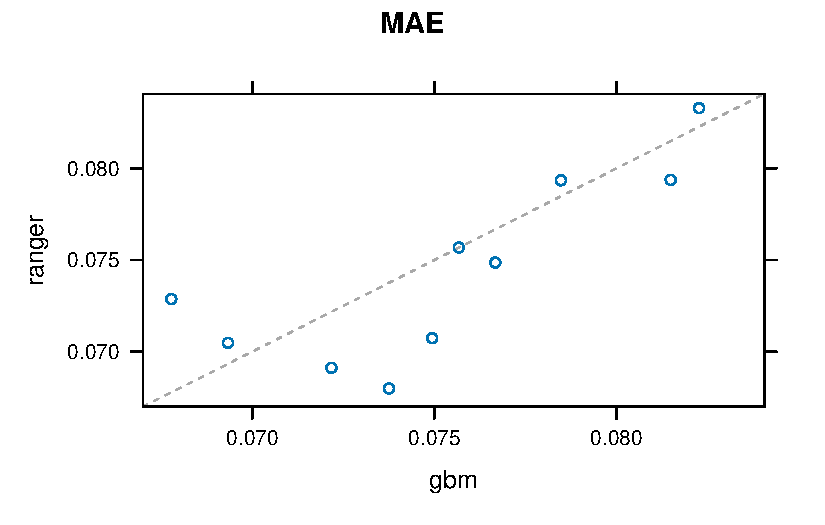
\includegraphics{MachineLearning_StaticPatterNN_Report_files/figure-pdf/ensemble-model-1.pdf}

\begin{Shaded}
\begin{Highlighting}[]
\CommentTok{\# Create the ensemble model}
\NormalTok{ensembleModel }\OtherTok{\textless{}{-}} \FunctionTok{caretEnsemble}\NormalTok{(}
\NormalTok{    modelsList,}
    \AttributeTok{metric =} \StringTok{"Rsquared"}\NormalTok{,}
    \AttributeTok{trControl =}\NormalTok{ trained\_control)}
\end{Highlighting}
\end{Shaded}

\begin{verbatim}
+ Resample01: parameter=none 
- Resample01: parameter=none 
+ Resample02: parameter=none 
- Resample02: parameter=none 
+ Resample03: parameter=none 
- Resample03: parameter=none 
+ Resample04: parameter=none 
- Resample04: parameter=none 
+ Resample05: parameter=none 
- Resample05: parameter=none 
+ Resample06: parameter=none 
- Resample06: parameter=none 
+ Resample07: parameter=none 
- Resample07: parameter=none 
+ Resample08: parameter=none 
- Resample08: parameter=none 
+ Resample09: parameter=none 
- Resample09: parameter=none 
+ Resample10: parameter=none 
- Resample10: parameter=none 
Aggregating results
Fitting final model on full training set
\end{verbatim}

\begin{Shaded}
\begin{Highlighting}[]
\NormalTok{greedy\_ensemble }\OtherTok{\textless{}{-}} \FunctionTok{caretEnsemble}\NormalTok{(}
\NormalTok{    modelsList,}
    \AttributeTok{metric =} \StringTok{"Rsquared"}\NormalTok{,}
    \AttributeTok{trControl =} \FunctionTok{trainControl}\NormalTok{(}
        \AttributeTok{number =} \DecValTok{2}\NormalTok{,}
        \AttributeTok{summaryFunction =}\NormalTok{ defaultSummary))}
\FunctionTok{summary}\NormalTok{(greedy\_ensemble)}
\end{Highlighting}
\end{Shaded}

\begin{verbatim}
The following models were ensembled: ranger, gbm, xgbTree, ranger.1 
They were weighted: 
-0.0136 -0.3646 0.4103 0.2371 0.7454
The resulting Rsquared is: 0.8644
The fit for each individual model on the Rsquared is: 
   method  Rsquared RsquaredSD
   ranger 0.7582122 0.03730201
      gbm 0.7605502 0.04228567
  xgbTree 0.7848171 0.02770065
 ranger.1 0.7586064 0.03927131
\end{verbatim}

\begin{Shaded}
\begin{Highlighting}[]
\FunctionTok{summary}\NormalTok{(ensembleModel)}
\end{Highlighting}
\end{Shaded}

\begin{verbatim}
The following models were ensembled: ranger, gbm, xgbTree, ranger.1 
They were weighted: 
-0.0136 -0.3646 0.4103 0.2371 0.7454
The resulting Rsquared is: 0.838
The fit for each individual model on the Rsquared is: 
   method  Rsquared RsquaredSD
   ranger 0.7582122 0.03730201
      gbm 0.7605502 0.04228567
  xgbTree 0.7848171 0.02770065
 ranger.1 0.7586064 0.03927131
\end{verbatim}

\begin{Shaded}
\begin{Highlighting}[]
\FunctionTok{varImp}\NormalTok{(modelsList[[}\DecValTok{1}\NormalTok{]])}
\end{Highlighting}
\end{Shaded}

\begin{verbatim}
ranger variable importance

  only 20 most important variables shown (out of 68)

                              Overall
rel_occ_Ncells               100.0000
moran                         31.3160
D_AOO_a                       30.5780
x_intercept                   13.5313
AOO                           10.8605
rel_relCirc                   10.0310
datasetBirds_atlas_EBBA        8.3218
mean_prob_cooccur              5.8013
circ                           4.0829
Dist_centroid_to_COG           3.2521
BetaSR_sp                      2.4306
Southernness                   1.2711
sp_centr_lat                   1.1850
sp_centr_lon                   1.1442
AlphaSR_sp                     1.0600
Primary.LifestyleTerrestrial   0.9313
Westernness                    0.8581
widthMinRect                   0.8572
IUCNEN                         0.8258
HabitatWetland                 0.7043
\end{verbatim}

\begin{Shaded}
\begin{Highlighting}[]
\FunctionTok{varImp}\NormalTok{(modelsList[[}\DecValTok{2}\NormalTok{]])}
\end{Highlighting}
\end{Shaded}

\begin{verbatim}
gbm variable importance

  only 20 most important variables shown (out of 68)

                       Overall
D_AOO_a                100.000
AOO                     97.762
rel_occ_Ncells          87.202
moran                   36.706
x_intercept             28.010
circ                    24.783
BetaSR_sp               21.615
rel_relCirc             17.270
GlobRangeSize_m2        14.858
minDist_toBorder_centr   7.227
mean_prob_cooccur        7.065
widthMinRect             6.406
rel_maxDist              5.588
sp_centr_lat             4.900
Southernness             4.573
elonMinRect              4.301
Hand.Wing.Index          4.169
AlphaSR_sp               4.020
Dist_centroid_to_COG     3.802
Westernness              3.393
\end{verbatim}

\begin{Shaded}
\begin{Highlighting}[]
\FunctionTok{varImp}\NormalTok{(modelsList[[}\DecValTok{3}\NormalTok{]])}
\end{Highlighting}
\end{Shaded}

\begin{verbatim}
xgbTree variable importance

  only 20 most important variables shown (out of 68)

                       Overall
AOO                    100.000
D_AOO_a                 53.534
mean_prob_cooccur       34.269
rel_occ_Ncells          25.974
moran                   23.957
circ                    20.244
GlobRangeSize_m2        14.701
BetaSR_sp               12.402
rel_relCirc             12.276
Dist_centroid_to_COG     9.573
minDist_toBorder_centr   4.279
x_intercept              4.194
Westernness              3.791
sp_centr_lon             2.533
Hand.Wing.Index          1.895
widthMinRect             1.443
Southernness             1.412
AlphaSR_sp               1.351
rel_elonRatio            1.334
sd_PC2                   1.269
\end{verbatim}

\subsubsection{Train Neural Network}\label{train-neural-network}

We will train 10 sets of neural networks (one for each resample of the
data splitting)

\begin{Shaded}
\begin{Highlighting}[]
\ControlFlowTok{for}\NormalTok{ (resamp }\ControlFlowTok{in} \FunctionTok{seq\_along}\NormalTok{(indices)) \{}
\NormalTok{    train\_df }\OtherTok{\textless{}{-}}\NormalTok{ dat\_v2[indices[[resamp]], ] }\CommentTok{\# 826 rows}
\NormalTok{    test\_df }\OtherTok{\textless{}{-}}\NormalTok{ dat\_v2[}\SpecialCharTok{{-}}\NormalTok{indices[[resamp]], ] }\CommentTok{\# 204 rows}

\NormalTok{    nn\_fit }\OtherTok{\textless{}{-}} \FunctionTok{dnn}\NormalTok{(Jaccard }\SpecialCharTok{\textasciitilde{}}\NormalTok{ .,}
        \AttributeTok{data =}\NormalTok{ train\_df }\SpecialCharTok{\%\textgreater{}\%} \FunctionTok{select}\NormalTok{(Jaccard, AOO, D\_AOO\_a, IUCN),}
        \AttributeTok{validation =} \FloatTok{0.2}\NormalTok{,}
        \AttributeTok{hidden =} \FunctionTok{c}\NormalTok{(}\DecValTok{50}\NormalTok{L, }\DecValTok{50}\NormalTok{L, }\DecValTok{50}\NormalTok{L, }\DecValTok{50}\NormalTok{L),}
        \AttributeTok{activation =} \StringTok{"relu"}\NormalTok{,}
        \AttributeTok{loss =} \StringTok{"mse"}\NormalTok{,}
        \AttributeTok{lr =} \FloatTok{0.0001}\NormalTok{,}
        \AttributeTok{epochs =} \DecValTok{6000}\NormalTok{L,}
        \AttributeTok{lr\_scheduler =} \FunctionTok{config\_lr\_scheduler}\NormalTok{(}\StringTok{"reduce\_on\_plateau"}\NormalTok{, }\AttributeTok{patience =} \DecValTok{10}\NormalTok{, }\AttributeTok{factor =} \FloatTok{0.5}\NormalTok{),}
        \AttributeTok{plot =} \ConstantTok{TRUE}\NormalTok{,}
        \AttributeTok{tuning =} \FunctionTok{config\_optimizer}\NormalTok{(}\StringTok{"adam"}\NormalTok{),}
        \AttributeTok{verbose =} \ConstantTok{TRUE}\NormalTok{,}
        \AttributeTok{bootstrap =} \DecValTok{1000}
\NormalTok{    )}

    \FunctionTok{analyze\_training}\NormalTok{(nn\_fit)}

\NormalTok{    predictions }\OtherTok{\textless{}{-}} \FunctionTok{predict}\NormalTok{(nn\_fit, test\_df)}

    \FunctionTok{plot}\NormalTok{(test\_df}\SpecialCharTok{$}\NormalTok{Jaccard, predictions)}

    \FunctionTok{summary}\NormalTok{(nn\_fit)}
\NormalTok{\}}
\end{Highlighting}
\end{Shaded}




\end{document}
